\glsresetall
\chapter{Ergebnisse}
\label{sec:Ergebnisse}

In diesem Kapitel präsentiere ich meine \gls{gt} über die Entstehung und Auswirkungen von Entwurfsentscheidungen in SeqAn vor und formuliere allgemeinere sich daraus ergebende Erkenntnisse. Bestandteil dieser Theorie sind Usability-Probleme, die es zu beseitigen gilt. Die dafür notwendigen Maßnahmen und deren Umsetzung stelle ich im zweiten Teil dieses Kapitels vor. Abschließend bespreche ich die Güte meiner Forschung und die Validierung bzw. Verallgemeinerbarkeit meiner Forschungsergebnisse.

Das darauf folgende, letzte Kapitel fasst meine Arbeit in seiner Gesamtheit zusammen und stellt Vorschläge für ein weiteres Vorgehen vor.

\bigskip

% Wie ich bereits im \sref{sec:gtm-informatik} dargelegt habe, ist der Gebrauch der \gls{gtm} in der Informatik mehr als rar. Genauer gesagt ist mir keine Studie bekannt, in der die \gls{gtm} vollständig, d.h. samt selektivem Kodieren und Darstellung der Ergebnisse in Form einer Story, angewendet wurde. Daher möchte ich um Verständnis bitten, sollte die im Folgenden präsentierte Story nicht ``protokollgetreu'' sein.

\begin{comment}
GT starke Ähnlichkeit mit paradigmatischem Modell. Jedoch waren Strategien nicht immer ersichtlich in den Daten. Daher Platzierung unterhalb
Theorie: Inspiriert durch das paradigmatische Modell.
Freiheiten nach Glaser



Nur Fokus auf Doku und \code{Templatemetaprogrammierung}\citepurl{apiua://code/-9223372036854775515} \code{Erwartungskonformität}\citepurl{sec:schwierigkeiten-breite}
da sonst einfach zu komplex wenn man empirische Verfahren nutzt \cite{SIGCHI:2009up}



Beim selektiven Kodieren eine ganze Menge weggefallen: z.B. \code{Langjähriger sporadischer Gebrauch}
Betroffene arbeiten nur selten mit SeqAn dafür aber seit Jahren mit SeqAn.
Die Anwender geben an, nicht erfahren/kompetent im Umgang mit SeqAn zu sein.
Ist das normal? Also auch bei anderer Software?
und
\code[apiua://code/-9223372036854775559]{Lernen / Vertiefen für Abschlussarbeit}
\end{comment}







\section[Theorie: Folgen von SeqAn-Entwurfsentscheidungen]{Theorie über die Entstehung und Auswirkungen von Entwurfsentscheidungen in SeqAn}
\label{sec:gt}

In diesem Abschnitt präsentiere ich meine \gls{gt} über das Zustandekommen von Entwurfsentscheidungen und deren Auswirkungen auf die API-Usability von SeqAn. Dabei beleuchte ich besonders die sich als außerordentlich wichtig herausgestellte \code{apiua://code/-9223372036854775515}\footnote{Zur Erinnerung: Die Kode-/Konzept-/Kategorie-Bezeichner können angeklickt werden. Sie sind verlinkt mit meinen Forschungsdaten. In dieser Darstellung der Theory nenne ich nur einige Phänomene von Konzepten. \textbf{Alle gefundenen Phänomene können in den verlinkten Forschungsdaten nachgelesen werden.} Die Farben geben Aufschluss über die Zusammengehörigkeit von Konzepten und werden durch einen semi-transparenten Kreis (\codebullet{apiua://code/-9223372036854774813}) dargestellt. Ein vollfarbiger Kreis (\codebullet{apiua://code/-9223372036854774814}) markiert besonders wichtige Konzepte. Die Notation wird ausführlich im \sref{sec:notationen} ab Seite \pageref{sec:notationen} beschrieben.}.

\fref{fig:research-gt} visualisiert meine Theorie. Gruppiert sind dabei die gefundenen bzw. entwickelten Konzepte in Form der fünf Hauptkategorien \code{apiua://code/-9223372036854775281}, \code{apiua://code/-9223372036854774893}, \code{apiua://code/-9223372036854774939}, \code{apiua://code/-9223372036854775414} und \code{apiua://code/-9223372036854774875}, wobei \code{apiua://code/-9223372036854775633} die Kernkategorie bildet.

Ich präsentiere meine \gls{gt} in Form einer \textit{Story}, bei der ich auf alle oben genannten Kategorien eingehen werde. Nicht alle Erkenntnisse sind datengetrieben im strengen Sinne der \gls{gtm} zu Stande gekommen. Ein Teil meiner Theorie basiert auf einer technisch-deduktiven Argumentation. Das heißt, habe ich ein Konzept in den Daten erst einmal erkennen können, reichten in solchen Fällen bereits Deduktionsschritte basierend auf existierenden wissenschaftlichen Erkenntnisse, um eben jene Konzepte hinreichend valide zu untermauern. Aussagen mit einem hohen technisch-deduktiven Anteil werden mit \theorybasis{td} ausgezeichnet und sind weniger stark in den aufgezeichneten Daten verankert. Aussagen, die beide Argumentationsstile kombinieren, werden durch \theorybasis{both} gekennzeichnet.

\begin{comment}
\begin{itemize}
%\itemsep1pt\parskip0pt\parsep0pt
  \item[] \code{Konzept}\theorybasis{dd}, das hauptsächlich auf einer datengetriebenen Argumentation basiert
  \item[] \code{Konzept}\theorybasis{td}, das hauptsächlich auf einer technisch-deduktiven Argumentation basiert
  \item[] \code{Konzept}\theorybasis{both}, das sowohl auf einer datengetriebenen als auch auf einer technisch-deduktiven Argumentation basiert
\end{itemize}
\end{comment}


\newgeometry{inner=2cm,outer=1.5cm,top=1.5cm,bottom=1.5cm}
\thispagestyle{empty}
\begin{landscape}
\begin{figure}
  \centering
    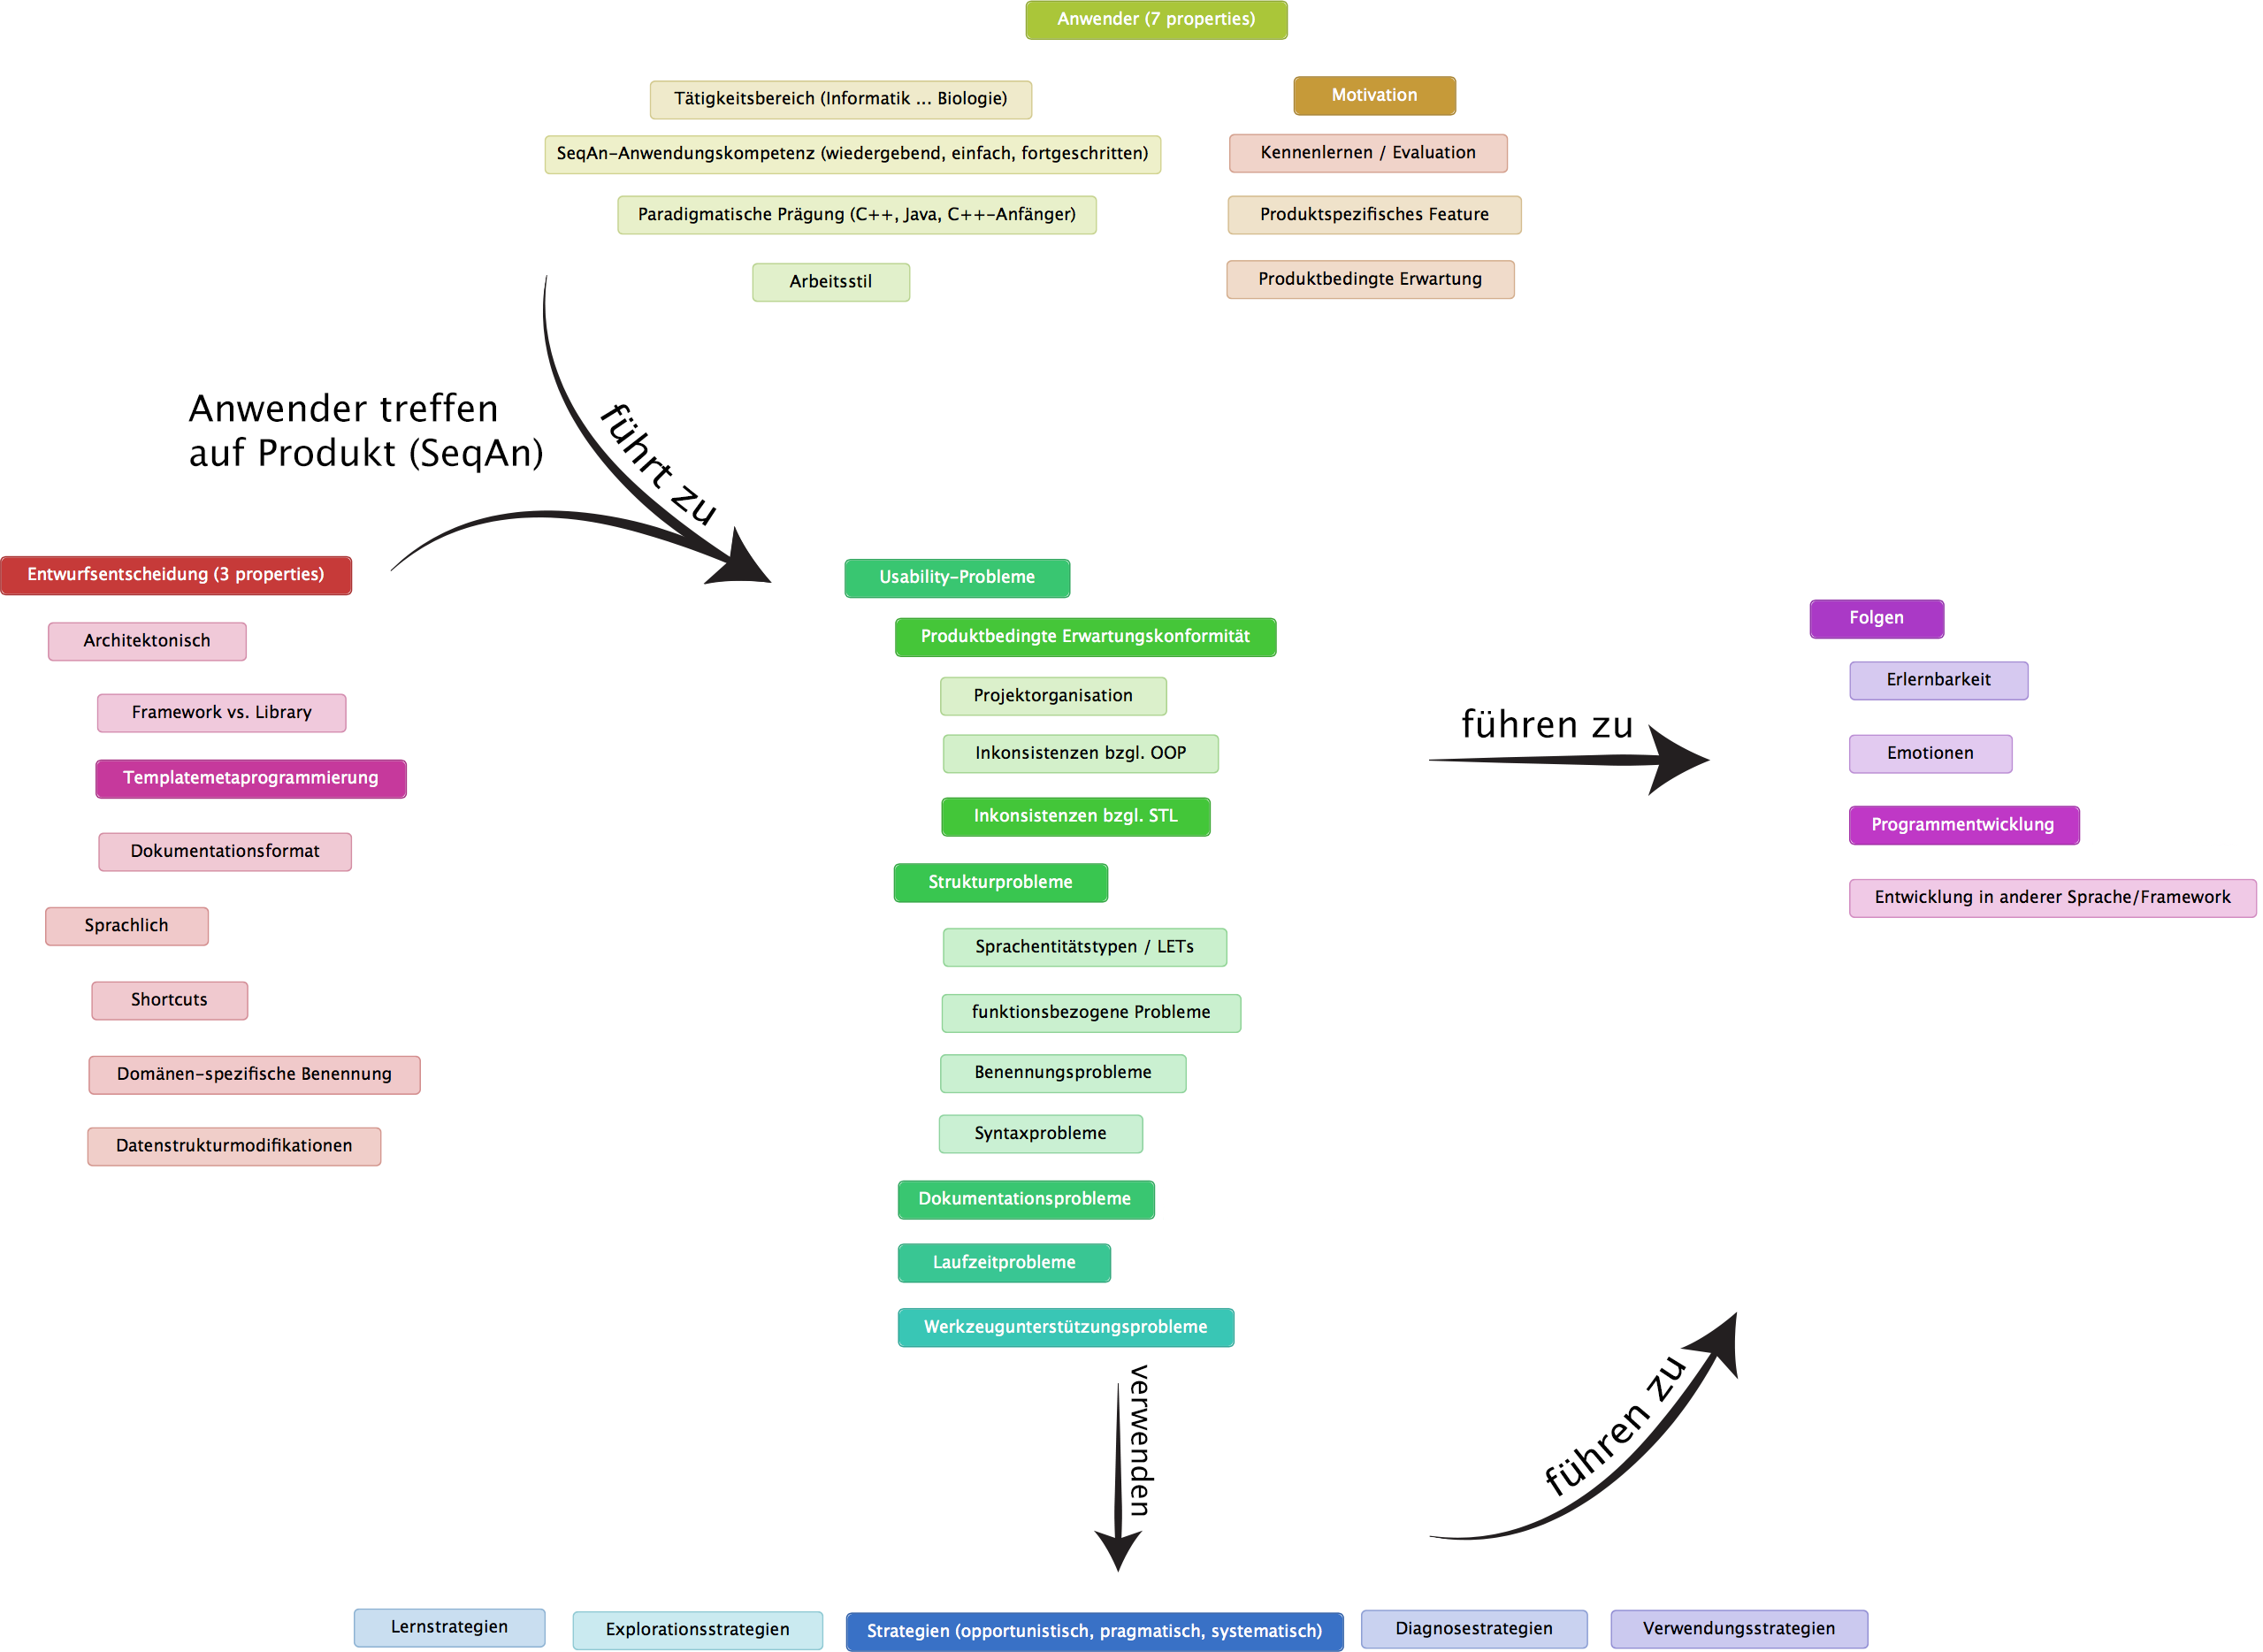
\includegraphics[width=0.8\linewidth]{Figures/research/gt.png}
  \caption[Theorie: Folgen von SeqAn-Entwurfsentscheidungen]{Die Theorie über die Entstehung und Auswirkungen von Entwurfsentscheidungen in SeqAn besteht aus fünf Hauptkategorien, die in Beziehung stehen und dem paradigmatischen Modell ähneln: \code{apiua://code/-9223372036854775281} beschreibt den Entwurf von SeqAn. Mit diesem sind SeqAns \code{apiua://code/-9223372036854774893} konfrontiert, was zu einer Reihe von \code[apiua://code/-9223372036854774939]{Usability-Problemen} führt. Zu Bewältigung kommen häufig \code{apiua://code/-9223372036854775414} zum Einsatz, deren Resultat mit den \code{apiua://code/-9223372036854774875} beschrieben werden.}
  \label{fig:research-gt}
\end{figure}
\end{landscape}
\restoregeometry



\subsection[Anwender]{\code{apiua://code/-9223372036854774893}}

Diese Kategorie beschreibt den Anwender von SeqAn und umfasst alle relevanten Eigenschaften, die zu dessen Charakterisierung notwendig sind. Die API-Anwender zu verstehen ist existenziell notwendig, um die Usability einer API bewerten zu können. Denn Usability-Probleme entstehen erst durch die Verwendung eines Systems durch seine Anwender.

Basierend auf den Ergebnissen meiner \gls{gtm}-Analyse und meiner im \sref{sec:phase1} vorgestellten Beseitigung grober Usability-Probleme, habe ich die folgenden relevanten Eigenschaften entdeckt\footnote{Um Verwunderungen in Bezug auf das von mir verwendete Vokabular auszuräumen: In der Präsentation meiner \gls{gt} verwende ich Verben wie ``beobachten'', ``suchen'' und ``entdecken'', weil dies der Philosophie der \gls{gtm} entspricht \citep[siehe \sref{sec:gtm} und][]{Glaser:1967ts}.}:
\begin{itemize}
  \item[\codebullet{apiua://code/-9223372036854775596}] \textbf{\codetext{apiua://code/-9223372036854775596}} \\
  In welchem Gebiet ist der Anwender vornehmlich tätig? Die Anwenderschaft von SeqAn besteht --- von wenigen Ausnahmen abgesehen --- aus Informatikern, Bioinformatikern und in geringerem Umfang aus Biologen (siehe \sref{sec:results-users}).\citepurl{apiua://code/-9223372036854774893}
  
  Diese Eigenschaft ist wichtig für die weiteren Betrachtungen, da einzelne beobachtete Bioinformatiker\citepurl{apiua://survey/cd/2013-09-18T17:46:55.042+02:00/errorProneness} und Biologen vollständig zu der Gruppe der API-Endanwender gezählt werden. Diese Gruppe zeichnet sich durch einen opportunistischen Arbeitsstil aus.\theorybasis{both}\footnote{Lediglich bei den Cognitive-Dimensions-Fragebögen habe ich nach dem Arbeitsstil gefragt. Dort gab jedoch keiner der Befragten an, einen opportunistischen Arbeitsstil zu haben. Ich gehe davon aus, dass dieser als laienhaft wahrgenommen wird und daher die Frage nicht immer wahrheitsgemäß beantwortet wurde. Tatsächlich kann man in den Programmierfortschritten opportunistisches Verhalten erkennen. In einem Fall\citepurl{https://github.com/bkahlert/seqan-research/blob/master/raw/workshop12/workshop2012-data-20120906/diff/phr0d30hyzmq0xri/phr0d30hyzmq0xri_r00000046_2012-09-05T13-32-11\%2B0200.diff\#L9} wird ein unerwartetes Verhalten einfach durch das manuelle Heraufsetzen einer Zählvariablen umgangen, ohne dass die Dokumentation konsultiert wurde. Ein (anderer) Diskussionsteilnehmer\citepurl{https://github.com/bkahlert/seqan-research/blob/master/raw/workshop12/workshop2012-data-20120906/group-discussions/workshop'12\%20-\%20Interview\%20Gruppendiskussion\%20(2012-09-06T13-01-28\%2B0200).html\#L290} deutet mit seiner Aussage ``a metafunction and this double colon and a type or value behind'', die den Versuch vermissen lässt, Metafunktionen zu verstehen, ebenfalls auf ein opportunistisches Verhalten hin. Diese Beobachtungen, die im \sref{sec:personas} beschriebene Literatur zu \textit{Personas} \citep{clarke:DSP:2007:1080} und die im \sref{sec:euse} beschriebene Literatur zu \textit{\acrlong{euse}} \citep{Ko:2011el} lassen den Schluss zu, dass der opportunistische Arbeitsstil auch unter der SeqAn-Anwenderschaft signifikant vertreten ist.}
  
  \item[\codebullet{apiua://code/-9223372036854775600}] \textbf{\codetext{apiua://code/-9223372036854775600}} \\
  Der Arbeitsstil beschreibt, auf welche Weise Anwender arbeiten. Basierend auf der Arbeit von \cite{clarke:DSP:2007:1080} (siehe \sref{sec:personas}) unterscheide ich den \textit{opportunistischen}, \textit{pragmatischen} und \textit{systematischen} Arbeitsstil. Diese Eigenschaft ist für die Analyse von \code[apiua://code/-9223372036854775414]{Problemlösungsstrategien} relevant.\theorybasis{td}
  
  \item[\codebullet{apiua://code/-9223372036854775494}] \textbf{\codetext{apiua://code/-9223372036854775494}}\label{sec:paradigmatische-pragung} \\
  Von dieser Eigenschaft wurde in der Literatur nach meinem Kenntnisstand noch nicht berichtet. Sie beschreibt, durch welche Programmierparadigmen der Anwender geprägt sein kann.
  
  Erstmalig wurde ich auf diese Eigenschaft aufmerksam, als ich bei der Auswertung der Workshop'12-Fragebögen auf die folgenden Aussagen stieß:
  \begin{itemize}
    \item ``I’m noticing that of the constructs are different from what is common in the STL. This might be justified but it makes it *much* harder to learn.''\citepurl{https://github.com/bkahlert/seqan-research/blob/master/raw/workshop12/workshop2012-data-20120906/feedback/feedback.tsv\#L5}
    \item ``Why don't you use the naming convention (for iterators) used also by STL?''\citepurl{https://github.com/bkahlert/seqan-research/blob/master/raw/workshop12/workshop2012-data-20120906/feedback/feedback.tsv\#L23}
    \item ``Not STL-like. Tries to reinvent STL with global function and it ads a lot of complexity that seems unnecessary.''\citepurl{https://github.com/bkahlert/seqan-research/blob/master/raw/workshop12/workshop2012-data-20120906/feedback/feedback.tsv\#L51}
  \end{itemize}

  
  Ich konnte grob die folgenden zwei Prägungen erkennen: \textit{Java-Objektorientierung} und \textit{C++-/STL-Objektorientierung}. Beiden Prägungen ist gemein, dass sie sich mit der objektorientierten Programmierung befassen. Sie unterscheiden sich jedoch in der Strenge. Während Java streng objektorientiert und sozusagen ``mono-paradigmatisch'' ist, vermischen sich bei der C{}\verb!++!-Objektorientierung verschiedene Paradigmen --- insbesondere das der Templatemetaprogrammierung, welche durch die STL jedoch teilweise durch die Verwendung von \texttt{typedefs} verborgen wird. Beispielsweise ist die \texttt{string}-Klasse\footnote{\url{http://www.cplusplus.com/reference/string/string/}} nichts weiter als ein \mintinline{cpp}{typedef basic_string<char>}.
  
  Diese Prägung habe ich in meiner Datenerhebung nicht explizit, jedoch indirekt über Fragestellungen zu Fertigkeiten mit bekannten Programmiersprachen erfragt. In Zusammenhang mit der Nennung verschiedener Usability-Probleme war es häufig nicht schwierig, auf die paradigmatische Prägung zu schließen. Gab ein Anwender\citepurl{https://github.com/bkahlert/seqan-research/blob/master/raw/workshop12/workshop2012-data-20120906/feedback/feedback.tsv\#L7} beispielsweise an, die besten Kenntnisse in Bezug auf Java zu haben und bezeichnete sich dieser auch noch als Java-Entwickler, wurde klar, dass er eine \code[apiua://code/-9223372036854775494]{Java-objektorientierte Prägung} besaß.
  
  Diese Eigenschaft ist ursächlich für eine Reihe von \code[apiua://code/-9223372036854774939]{Usability-Problemen}.
  
  \item[\codebullet{apiua://code/-9223372036854774938}] \textbf{\codetext{apiua://code/-9223372036854774938}} \\
  Diese Eigenschaft beschreibt, in welcher Form SeqAn eingesetzt werden kann. Zu beobachten war, dass Anwender SeqAn entweder zur Implementierung von \textit{Hilfsprogrammen}\citepurl{apiua://code/-9223372036854775587} oder zur Entwicklung einer ganzen \textit{Pipeline}\footnote{Für die Sequenzanalyse werden häufig mehrere Phasen durchlaufen. Dazu gehört u.a. die Vorbereitung der Daten (\textit{Proprocessing}) und die Visualisierung der Analyseergebnisse. Die technische Aneinanderreihung dieser Phasen wird häufig als \textit{Pipeline} bezeichnet.}\citepurl{apiua://code/-9223372036854775598} nutzten. Dies wurde auch in persönlichen Gesprächen mit den Workshop-Teilnehmer bestätigt.%\footnote{Tatsächlich wird SeqAn auch innerhalb von Abschlussarbeiten verwendet, worauf allerdings nicht mein Fokus lag.}
  
  Die Relevanz dieser Eigenschaft wird weiter unten deutlich.
  
   
  
  \item[\codebullet{apiua://code/-9223372036854775446}] \textbf{\codetext{apiua://code/-9223372036854775446}} \\
  Diese Eigenschaft beschreibt, welche Erfahrung Anwender im Gebrauch von SeqAn besitzen können. Differenziert wird diese Eigenschaft in Anlehnung an die verschiedenen Tutorial-Übungsaufgaben-Schwierigkeitsgrade, die im \sref{sec:tutorials-improve} beschrieben und für meine Zwecke hinreichend validiert sind\theorybasis{both}. Sie lauten:
  
  \begin{description}
    \item[Lernen] Der Anwender lernt SeqAn erst kennen und kann bestenfalls den SeqAn-Anwendungscode so weit verstehen, dass er einfache Anpassungen vornehmen kann. 
    \item[Anwendung] Der Anwender beherrscht SeqAn hinreichend, um existierenden Code neu komponieren und mehrzeilige Anwendungen selbstständig implementieren zu können.
    \item[Beherrschung] Der Anwender verfügt über genügend Kenntnisse, dass er selbstständig SeqAn-Anwendungen für seinen eigenen Bedarf schreiben kann. 
  \end{description}
  
  Meine Betrachtungen beschränken sich weitgehend auf Anwender, die SeqAn nicht beherrschen und dürften für Anwender mit guter SeqAn-Beherrschung nur geringe Gültigkeit haben.
  
  \item[\codebullet{apiua://code/-9223372036854775599}] \textbf{\codetext{apiua://code/-9223372036854775599}} \\
  Die Eigenschaft befasst sich mit den Gründen, aus denen sich Anwender mit SeqAn befassen. Diese Eigenschaft verfügt über die folgenden Untereigenschaften:
  
  \begin{itemize}
    \item[\codebullet{apiua://code/-9223372036854775407}] \textbf{\codetext{apiua://code/-9223372036854775407}} \\
    Es handelt sich hierbei um eine boolesche Eigenschaft. Sie gibt Auskunft darüber, ob potentielle Anwender SeqAn zunächst kennen lernen wollen. Dieses Kennenlernen kann zielgerichtet sein. In diesem Fall spreche ich von Evaluation. Die Anwender gaben wenig überraschend an, SeqAn für die Sequenzanalyse zu verwenden und SeqAns Eignung zu diesem Zweck überprüfen zu wollen. Ein Anwender\citepurl{apiua://code/-9223372036854775547} hatte besonders konkrete Vorstellungen. Er hatte bereits eine entsprechende Pipeline in der Programmiersprache C entwickelt und wollte prüfen, inwiefern er diese nach SeqAn portieren kann, um von SeqAns \code[apiua://code/-9223372036854775552]{Performance-Eigenschaft} profitieren zu können.
    
    \item[\codebullet{apiua://code/-9223372036854774827}] \textbf{\codetext{apiua://code/-9223372036854774827}} \\
    Diese Eigenschaft beschreibt Erwartungen, die beim Anwender durch das Produkt --- also durch SeqAn --- geweckt werden können. Wie noch weiter unten erläutert wird, weckt SeqAn die folgenden Erwartungen:
    
    \begin{itemize}
      \item[\codebullet{apiua://code/-9223372036854774830}] \textbf{\codetext{apiua://code/-9223372036854774830}} \\
      Erwartung, dass es sich bei SeqAn um eine Softwarebibliothek handelt, die in das eigene Projekt eingebunden werden kann. Interessanterweise wurde ich auf diese Erwartung nur durch persönliche Gespräche --- vielfach --- aufmerksam. In meinen technisch erfassten Daten ist diese Erwartung nicht ohne Weiteres zu finden. Verantwortlich mache ich dafür das Umfeld, in dem die Datenaufzeichnungen stattfanden. Diese waren nämlich stets moderiert (Workshop bzw. Projektseminar, siehe \sref{sec:rahmenbedingungen}) und hatten nicht den Fokus auf die Integration von SeqAn in einem eigenen Projekt, sondern auf das Erlernen von SeqAn in einer vergleichsweise praxisfremden Umgebung.\theorybasis{both}
      
%      \item[\codebullet{apiua://code/-9223372036854775568}] \textbf{\codetext{apiua://code/-9223372036854775568}} \\
%      Erwartung, dass SeqAn für ein großes Funktionsspektrum verfügt.
      
      \item[\codebullet{apiua://code/-9223372036854775298}] \textbf{\codetext{apiua://code/-9223372036854775298}} \\
      Erwartung, dass die mit SeqAn entwickelten Anwendungen besonders schnell sind.\citepurl{apiua://survey/cd/2013-09-19T11:51:16.616+02:00/provisionality}
      
      \item[\codebullet{apiua://code/-9223372036854775311}] \textbf{\codetext{apiua://code/-9223372036854775311}} \\
      Erwartung, dass SeqAn einfach in der Anwendung ist.\citepurl{apiua://survey/cd/2013-09-19T11:51:16.616+02:00/roleExpressiveness}\citepurl{apiua://survey/cd/2013-09-18T17:44:46.060+02:00/learningStyle}
    \end{itemize}
        
    \item[\codebullet{apiua://code/-9223372036854774826}] \textbf{\codetext{apiua://code/-9223372036854774826}} \\
    Die Eigenschaft unterscheidet sich von \codebullet{apiua://code/-9223372036854774827}{produktbedingen Erwartungen} in dem Grad der Gewissheit. Sie beschreibt keine Erwartung, sondern das Wissen um eine Eigenschaft und betrifft hauptsächlich Anwender, die sich bereits von den Vorzügen der folgenden Eigenschaft überzeugen konnten und aus diesem Grund SeqAn einsetzen.
    
    \begin{itemize}
%      \item[\codebullet{apiua://code/-9223372036854775297}] \textbf{\codetext{apiua://code/-9223372036854775297}} \\
%      Wissen um das große Funktionsspektrum von SeqAn.
      
      \item[\codebullet{apiua://code/-9223372036854775552}] \textbf{\codetext{apiua://code/-9223372036854775552}} \\
      Wissen um die hohe Performance von mit SeqAn entwickelten Programmen.\citepurl{apiua://survey/cd/2013-09-18T17:50:13.425+02:00/mainPurpose}\citepurl{apiua://groupDiscussion/workshop\%2712+-+Interview+Gruppendiskussion+\%282012-09-06T13-01-28\%2B0200\%29.html/li/1}
    \end{itemize}
    
    Die auffälligste Beobachtung ist, dass in keiner meiner Datenerhebungen ein Proband von der Benutzerfreundlichkeit von SeqAn berichtete, obwohl es die dazugehörige Erwartung gibt.
  \end{itemize}  
  
\end{itemize}




\subsection[Entwurfsentscheidungen]{\code[apiua://code/-9223372036854775281]{Entwurfsentscheidungen}}
\label{sec:gt-entwurfsentscheidungen}

SeqAn wurde von Andreas Gogol-Döring im Rahmen seiner Dissertation ``SeqAn --- A Generic Software Library for Sequence Analysis'' \citep{GogolDoring:2009vz} entwickelt. Auf der Grundlage seiner Arbeit habe ich die Kategorie \code[apiua://code/-9223372036854775281]{Entwurfsentscheidungen} erarbeitet, welche alle Entscheidungen auf Seiten der API-Entwickler beschreiben können soll, die den Entwurf von SeqAn prägen. Unterschieden wird dabei grundsätzlich in \code[apiua://code/-9223372036854774919]{architektonische} und \code[apiua://code/-9223372036854774918]{sprachliche Entwurfsentscheidungen}. Diese Unterscheidung stammt von \cite{Stylos:2007ip} (siehe \fref{fig:APIDesignDecisions} auf Seite \pageref{fig:APIDesignDecisions}).

Entwurfsentscheidungen können mit Hilfe der folgenden Eigenschaften charakterisiert werden:

\begin{itemize}
  \item[\codebullet{apiua://code/-9223372036854774864}] \textbf{\codetext{apiua://code/-9223372036854774864}} \\
  Diese Eigenschaft beschreibt das Ziel, mit der eine Entwurfsentscheidung getroffen wurde. Entdeckte Ziele sind \textit{Performance} und \textit{Usability}. Andere Ziele wie \textit{Simplizität} habe ich unter \textit{Usability} subsummiert.
  
  \item[\codebullet{apiua://code/-9223372036854774942}] \textbf{\codetext{apiua://code/-9223372036854774942}} \\
  Diese Eigenschaft beschreibt die Motivation der Entwurfsentscheidung. Dabei kann es sich entweder um die Absicht handeln, das erklärte Ziel zu erreichen (\textit{Zielverfolgungsabsicht}) oder um eine \textit{notwendige Folgeentscheidung}, die sich aus einer vorangegangenen Entwurfsentscheidung ergibt. Ist Letzteres der Fall, so kann es ein Entwurfsentscheidungsziel geben --- und zwar dann, wenn der API-Entwickler beispielsweise etwas kompensieren muss. Die weiter unten besprochene \code[apiua://code/-9223372036854775281]{Folge-Entwurfsentscheidung} \code{apiua://code/-9223372036854775412} diente dazu, die Usability zu steigern, indem Polymorphie ermöglicht wurde. Dieser Schritt war jedoch nur notwendig, weil durch den Einsatz von \code{apiua://code/-9223372036854775515} und den Verzicht auf objektorientierte Programmierung Polymorphie zunächst nicht mehr nutzbar gewesen ist. 
  
  \item[\codebullet{apiua://code/-9223372036854774839}] \textbf{\codetext{apiua://code/-9223372036854774839}} \\
  Diese Eigenschaft beschreibt die Art, wie die Entwurfsentscheidung zustande kam bzw. umgesetzt wurde. Die entsprechende Dimension umfasst dabei das Spektrum von \textit{implizit} bis \textit{explizit-empirisch}.
  
  \begin{description}
    \item[Implizite] Entwurfsentscheidungen sind solche, die unbewusst getroffen wurden. Diese Art ist häufig anzutreffen, wenn es sich um eine notwendige Folgeentscheidung handelt. In dieser Konstellation hat der API-Entwickler nicht erkannt, dass er gerade eine Entwurfsentscheidung trifft, was tendenziell ein weniger vorhersagbares Ergebnis bedingt.
    \item[Explizite-intuitive] Entwurfsentscheidungen sind solche, die zwar erkannt wurden, jedoch lediglich intuitiv getroffen wurden. Implizite und explizit-intuitive Entscheidungen bezeichne ich auch als \code{Bauchgefühlentscheidung}. \label{sec:bauch-usability}
    \item[Explizite-argumentative] Entwurfsentscheidungen unterscheiden sich von explizit-intuitiven Entwurfsentscheidungen dadurch, dass sie argumentiert werden. Als Argumente dienen u.a. Erfahrungen des API-Entwicklers oder Entwurfsentscheidungen, die von Dritten in anderen Produkten getroffen und adaptiert wurden.
    \item[Explizite-empirische] Entwurfsentscheidungen haben die höchste Wahrscheinlichkeit, das Entscheidungsziel zu erreichen. Die Wirksamkeit derartiger Entwurfsentscheidungen wird vom Entscheider empirisch belegt. Der empirische Wirkungsnachweis kann dabei selbst erbracht werden oder auf empirisches Untersuchen in verwandten Arbeiten fußen. 
  \end{description}
  
  Bei der vorgestellten Unterteilung handelt es sich um eine Dimension mit zwei Extremen und erlaubt viele Schattierungen. So sind die Grenzen zwischen den expliziten Entscheidungsgrundlagen fließend --- je nachdem, wie solide die Argumentation ist.
  
  Implizite Entwurfsentscheidungen sind weniger differenziert, denn das Fehlen der Explikation der Entscheidungsgrundlage lässt keine zuverlässige Unterscheidung zu.
\end{itemize}

\bigskip

In Bezug auf \code[apiua://code/-9223372036854775281]{Entwurfsentscheidungen} kann SeqAn also wie folgt beschrieben werden:

SeqAn wurde als quelloffene Softwarebibliothek (\textit{Library}) entworfen, welche auf C{}\verb!++! basiert und zum ultimativen \code{apiua://code/-9223372036854774864} die Geschwindigkeit (\textit{Performance}) von mit SeqAn entwickelten Programmen hatte. Ein weiteres \codetext{apiua://code/-9223372036854774864} war die Benutzerfreundlichkeit (\textit{Usability}) von SeqAn.

Diese Beschreibung, welche sich auch auf der SeqAn-Website\footnote{\url{http://www.seqan.de}} befindet, weckt auf \code[apiua://code/-9223372036854774893]{Anwenderseite} vier \code[apiua://code/-9223372036854774827]{produktbedingte Erwartungen}, von denen drei nicht erfüllt werden. Diese bezeichne ich informell gerne auch als \textit{die drei Urlügen / -täuschungen}. Die im Folgenden vorgestellten, unerfüllten \code[apiua://code/-9223372036854774827]{produktbedingten Erwartungen} bzw. \textit{Urlügen} basieren auf meinen Analysen der in \sref{sec:datenerhebung} vorgestellten Datenquellen, sowie der im vorherigen Absatz genannten Dissertation \citep{GogolDoring:2009vz} und einem längeren Telefonat mit Andreas Gogol-Döring \citep{GogolDoring:5iYhf2VJ}:

\begin{description}
  \item[1. Framework statt Softwarebibliothek]\label{sec:lie-library}\label{sec:library-vs-framework} (\code{apiua://code/-9223372036854774830}) \\
  SeqAn sollte eine Library sein, wurde jedoch als Framework entwickelt.
  
  Der Unterschied besteht in der Art, wie das ``architektonische Skelett'' der entwickelten Anwendungen durch die Library bzw. das Framework vorgegeben wird. Bei einer Library ist der API-Anwender weitgehend unbeeinflusst --- er bindet die durch die Library bereitgestellte Funktionalität lediglich ein. Bei einem Framework wird die Struktur der entwickelten Anwendungen weitgehend von dem Framework vorgegeben. \citep{Fairbanks:2006jw}
  
  Diese Form der Implementierung wird durch die \code[apiua://code/-9223372036854774919]{architektonische Entwurfsentscheidung} \code{apiua://code/-9223372036854775215} erfasst. Dabei handelt es sich nach meiner Einschätzung um eine \textit{implizite} Entscheidung, denn Gogol-Döring lässt in seiner Dissertation kein Bewusstsein vermuten, dass die folgenden Beobachtungen de facto zur Implementierung eines Frameworks führen\theorybasis{td}:
  
  \begin{itemize}
    \item SeqAn verwendet das plattformübergreifende Build-System \textit{CMake}\footnote{\url{http://www.cmake.org}}. Das hat zur Folge, dass SeqAn-Anwender Programme nur innerhalb dieses Systems entwickeln können. Eine Einbindung von SeqAn in das eigene C{}\verb!++!-Projekt --- durch Inkludierung einer entsprechenden Header-Datei --- ist \textit{nicht} vorgesehen.
    \item Die SeqAn-Entwickler nutzen Vorausdeklarationen (\textit{forward declarations}), um API-interne Abhängigkeiten aufzulösen. Diese werden durch ein, in das Build-System integriertes Python-Skript bei jedem Kompilieren automatisch generiert, was die Komplexität von Vorausdeklarationen verringert. Ein SeqAn-Anwender müsste für den Gebrauch von SeqAn als Library dieses Skript selbst ausführen.
    \item SeqAn verwendet eine dreigliedrige Organisation. Der \textit{Core} umfasst dabei alles, was zu SeqAn gehört. \textit{Extras} beinhaltet funktionale Erweiterungen, die weitgehend auf die Ergebnisse von Abschlussarbeiten zurückgehen. Ist ein Extra von großer Relevanz und genügt es nicht näher spezifizierten Qualitätsanforderungen, wird es in den Core aufgenommen. Schließlich gibt es noch die \textit{Sandboxes}. Jeder SeqAn-Anwender muss mit Hilfe eines Python-Skripts eine Sandbox erstellen. Innerhalb seiner Sandbox wiederum werden durch abermalige Python-Skript-Aufrufe \textit{Apps} erzeugt. Dabei handelt es sich um ein Skelett zur Entwicklung von SeqAn-Anwendungen. Die Verwendung des Python-Skripts ist obligatorisch, denn es erweitert das Build-System so, dass die selbst entwickelten SeqAn-Anwendungen / -Apps auch kompiliert werden können.
  \end{itemize}
  
  Aus diesen Gründen, ist SeqAn keine Library, sondern ein Framework. SeqAn kann nicht ohne weiteres in eigene Entwicklungsprojekte eingebunden werden, was in seiner Verwendung von CMake, dem Gebrauch von Vorausdeklarationen und der Vorgabe der Projektstruktur begründet ist. Damit wird massiv die oben beschriebene \code[apiua://code/-9223372036854774830]{Libraryerwartung} verletzt. Außerdem wird die \code[apiua://code/-9223372036854774938]{SeqAn-Einsatzform} eingeschränkt, wenn der Gebrauch als Library vorgezogen wird. Mehrere Workshop-Teilnehmer\citepurl{apiua://code/-9223372036854774830} gaben in mündlichen Gesprächen an, dass sie die Framework-Gestalt von SeqAn für inakzeptabel halten, da sie bereits ein eigenes Build-System betreiben und ein Wechsel nicht in Frage kommt. Dieses praxisrelevanten Äußerungen legen nahe, dass SeqAns Framework-Gestalt in der Praxis für viele potentielle Anwender ein Problem darstellt.\theorybasis{both}
  
  \item[2. Programmierparadigma]\label{sec:lie-oop} (\code{apiua://code/-9223372036854774809}) \\ 
  SeqAn nutzt als Programmiersprache C{}\verb!++!. Dies weckt Erwartungen, die im Konflikt zur anwenderseitigen \code[apiua://code/-9223372036854775494]{paradigmatischen Prägung} stehen können und u.a. folgende Wortmeldungen zur Folge haben:
  
  \begin{itemize}
    \item Ein Anwender mit einer \code[apiua://code/-9223372036854775494]{Java-Objektorientierungsprägung} bezeichnete SeqAn als ``Vergewaltigung der OO-Programmierung''\citepurl{apiua://survey/2011-09-14-T15:23:17.211+02:00}.
    \item Ein Anwender mit einer \code[apiua://code/-9223372036854775494]{C{}\texttt{++}-/STL-Objektorientierungsprägung} sagte: ``If SeqAn [just] had the same way of doing things like the STL''\citepurl{apiua://groupDiscussion/workshop\%2712+-+Interview+Gruppendiskussion+\%282012-09-06T13-01-28\%2B0200\%29.html/li/9}.
    \item Ein Anwender sagte allgemein im Zusammenhang mit der \code{apiua://code/-9223372036854775515}: ``[It's] not clear why you have to go through all this pain''\citepurl{apiua://groupDiscussion/workshop\%2712+-+Interview+Gruppendiskussion+\%282012-09-06T13-01-28\%2B0200\%29.html/li/14}.
  \end{itemize}
  
  Offenbar ``tickt'' SeqAn also anders, als es seine Anwender erwarten. Gogol-Döring traf die architektonische Entwurfsentscheidung, für die Entwicklung von SeqAn keine klassische Objektorientierung, sondern das Programmierparadigma \code{apiua://code/-9223372036854775515} zu verwenden.
  
  In seiner Dissertation stellt Gogol-Döring die Vorzüge der Templatemetaprogrammierung dar, ohne jedoch die Nachteile der Objektorientierung näher zu beleuchten. In dem Telefonat mit Gogol-Döring \citep{GogolDoring:5iYhf2VJ} erfragte ich diese:
  \begin{itemize}
    \item Gogol-Döring teilte mir mit, dass er kein Freund von objektorientierter Programmierung (OOP) sei. Als Beispiel nannte er, dass die Implementierung symmetrischer Operationen, wie der Addition, in der OOP auf eine ihm ``befremdliche'' Art gelöst würden --- nämlich durch Memberfunktionen und nicht durch ``symmetrische'', globale Funktionen.
%    \item -- Leere Basisklassen bekommen bei manchen Compilern ein Junk-Byte, weil leere Klassen nicht gehen $\rightarrow$ Speicherverbrauch
    \item Hauptargument für die Verwendung der Templatemetaprogrammierung war jedoch die dadurch hohe zu erreichende Performance. Zum Erreichen von Polymorphie werden in C{}\verb!++! virtuelle Funktionen benötigt. Welche Funktion tatsächlich zur Ausführung kommt, wird zur Laufzeit bestimmt --- und das kostet Rechenzeit (\textit{virtual lookup overhead}). Um die Bestimmung der aufzurufenden Funktion performance-steigernd zur Kompilierzeit zu berechnen (\textit{static binding}) und gleichzeitig Polymorphie zu erlauben, traf der SeqAn-Autor die Entscheidung, \code{apiua://code/-9223372036854775412} (\textit{Template Subclassing}) zu verwenden.
    \item Gogol-Döring experimentierte mit Möglichkeiten, eine hohe Performance mit Hilfe der OOP zu erreichen. Dies gelang ihm jedoch nicht.
%-- keine Shims-Funktionalität (Bereitstellung der Funktionalität für fremde Datentypen, z.B. STL-String)
  \end{itemize}
  
%  In Anbetracht dieser Argumentation und der seiner Dissertation kann man zusammenfassen, dass Gogol-Döring sich --- auch aus Präferenzgründen --- gegen OOP und für \code{apiua://code/-9223372036854775515} entschieden hat. Dabei handelt es sich um eine \textit{explizite-empirische} \code{apiua://code/-9223372036854775281}, denn der Autor konnte zeigen, dass er damit tatsächlich das \code{apiua://code/-9223372036854774864} \textit{Performance} erreichen konnte. Jedoch führt dieser Ansatz zu einer Reihe weiter unten beschriebener \code{apiua://code/-9223372036854774939}.
  
  \item[3. Usability]\label{sec:lie-usability} (\code{apiua://code/-9223372036854775311}) \\
  Gogol-Döring beschreibt als weiteres Entwurfsziel die \textit{Usability}. Um dies zu erreichen, entschloss sich der Autor zu der ebenfalls architektonischen Entwurfsentscheidung \code{apiua://code/-9223372036854775579}\footnote{Tatsächlich verfolgte Gogol-Döring mit der \code[apiua://code/-9223372036854775579]{Generischen Programmierung}, neben der \textit{Usability}, weitere Ziele wie \textit{Simplizität}, \textit{Generalisierbarkeit} und \textit{Erweiterbarkeit}. Für den Zweck meiner Arbeit reicht die zusammenfassende Betrachtung \textit{Usability}.}. Generische Funktionen lösen Probleme allgemeingültig. Kann ein Problem für bestimmte Eingaben effizienter gelöst werden (z.B. bei der Sortierung), kann eine spezialisierte Funktion implementiert werden. Der Compiler wählt beim Kompilieren die spezialisierteste Implementierung aus und bindet diese Funktion statisch, was die Performance von SeqAn sicherstellt \citep[Details siehe][]{GogolDoring:2009vz}.
% - open-closed principle
%  - neue Funktionalität ohne Codeänderung
%  - e.g. neue Spezialisierung, neue Funktionen
%  - Auslagerung in weitere header Dateien
  
  Ungünstigerweise werden generische Funktionen nicht als Memberfunktionen, sondern als globale Funktionen implementiert. Damit entfällt jedoch technisch die immer noch existierende inhaltliche Zusammengehörigkeit von Funktionen, was in der OOP durch die Klassenzugehörigkeit implementiert wird. Üblicherweise erwartet eine generische Funktion ihr \textit{Hauptobjekt} als erstes Argument. Schreibt man in OOP also \mintinline{java}{myString.length()}, lautet der gleiche Aufruf in SeqAn \mintinline{cpp}{length(myString)}. In SeqAn wird die inhaltliche Zusammengehörigkeit von Funktionen als \textit{global function interface} bezeichnet und nur noch in der Dokumentation beschrieben, was insbesondere \code{apiua://code/-9223372036854774819} behindert.
  
  Durch die globale Implementierung von generischen Funktionen, firmieren unterschiedliche Funktionen unter dem gleichen Namen im globalen Namespace. Entsprechend variabel ist auch deren Rückgabetyp. Den korrekten Rückgabetyp zu ermitteln, ist mühsam und fehlerträchtig. Um u.a. dieses Problem zu lösen, wurde die Entwurfsentscheidung \code{apiua://code/-9223372036854775514} getroffen. Dabei handelt es sich um Funktionen, die nicht zur Laufzeit, sondern zur Kompilierzeit ausgeführt werden. Sie werden dazu verwendet, den korrekten Typ für die Rückgabe einer generischen Funktion zu berechnen. Syntaktisch ähneln Metafunktionen allerdings Klassen, da Metafunktionen in SeqAn ebenfalls mit einem Großbuchstaben beginnen\theorybasis{td}. Da die SeqAn-Anwender über eine unpassende \code{apiua://code/-9223372036854775494} verfügen, führt dies zu \code[apiua://code/-9223372036854774939]{Usability-Problemen}, die weiter unten erläutert werden.
  
  \code{apiua://code/-9223372036854775579} und \code{apiua://code/-9223372036854775514} sind im Falle von SeqAn \textit{explizite-argumentative} \code[apiua://code/-9223372036854775281]{Entwurfsentscheidungen} mit dem \code{apiua://code/-9223372036854774864} \textit{Usability}. Ein empirischer Beleg für die Wirksamkeit der Entscheidungen fehlt. Stattdessen wird die Wirksamkeit nur unzureichend argumentativ an drei Stellen seiner Dissertation \citep{GogolDoring:2009vz} erbracht:
  \begin{itemize}
    \item In Unterkapitel 14.1 argumentiert der Autor, dass SeqAn lediglich eine geringe Anzahl von Techniken kombiniert, von denen jede nur eine begrenzte Komplexität (``limited complexity'') aufweist. Gleichzeitig räumt er aber ein, dass sein Ansatz als unüblich von den meisten Programmierern empfunden werden könnte und Fehlerausgaben der Compilers ``ziemlich'' schwer verständlich sind. % Darüber hinaus beschreibt er die durch \code{apiua://code/-9223372036854775412} ermöglichte Polymorphie als Vereinfachung.
    In dieser Betrachtung unterschätzt Gogol-Döring im erheblichen Maß die Auswirkungen seines Entwurfs.
    \item In Unterkapitel 14.2 argumentiert der Autor, dass der erfolgreiche Einsatz von SeqAn im Rahmen von Arbeiten innerhalb der Bioinformatik-Arbeitsgruppe die Usability bestätigt. Allerdings ignoriert er dabei, dass die meisten Anwender die Entwicklung von SeqAn miterlebten/-gestalteten und sich bei Problemen, direkt an den Autoren wenden konnten.
    \item In Kapitel 15 demonstriert Gogol-Döring die Re-Implementierung der Basisfunktionalität eines Bioinformatik-Werkzeugs. Damit stellt er allerdings lediglich unter Beweis, dass SeqAn für ihn selbst benutzbar ist. 
  \end{itemize}
  
%  Zusammenfassend kann man sagen, dass Gogol-Döring den Fehler begangen hat, die Usability von SeqAn nicht ausreichend belegt zu haben. Der größte Mangel besteht darin, die Anwender von SeqAn nicht ausreichend berücksichtigt zu haben.
  
  Die in Kapitel 15 angeklungene \code{Bauchgefühl-Usability} setzt sich in sämtlichen \code[apiua://code/-9223372036854774918]{sprachlichen Entwurfsentscheidungen} fort, d.h. all diese Entscheidungen sind \textit{implizit} oder \textit{explizit-intuitiv} --- werden also gar nicht oder nur intuitiv begründet:
  \begin{itemize}
    \item[\codebullet{apiua://code/-9223372036854775611}] \textbf{\codetext{apiua://code/-9223372036854775611}} \\
    Hierbei handelt es sich um C{}\verb!++!-\texttt{typedefs}, die eine einfachere Schreibweise von häufigen Templatespezialisierungen bereitstellen sollen. Beispiel: Das Shortcut \mintinline{cpp}{DnaString} kann anstelle von \mintinline{cpp}{String<Dna>} verwendet werden.
    
    \item[\codebullet{apiua://code/-9223372036854774848}] \textbf{\codetext{apiua://code/-9223372036854774848}} \\
    In SeqAn mischt Gogol-Döring Termini aus den Domänen Informatik (z.B. \texttt{Alloc}), Bioinformatik (z.B. \texttt{Alphabet}, \texttt{Gaps}) und Biologie (z.B. \texttt{Peptide}), was u.a. zum weiter unten erläuterten \code{apiua://code/-9223372036854775144} führt.\theorybasis{both}
    
    \item[\codebullet{apiua://code/-9223372036854774838}] \textbf{\codetext{apiua://code/-9223372036854774838}} \\
    Datenstrukturen können auf unterschiedliche Weise verändert werden. In SeqAn kommen verschiedene Ansätze zum Einsatz, die entlang zweier Dimensionen charakterisiert werden können\theorybasis{td}:
    \begin{description}
      \item[Direktheit] Werden Datenstrukturen direkt oder indirekt verändert?
      \item[Explizitheit] Werden Datenstrukturen explizit oder implizit verändert?
    \end{description}
    
    Es gibt also vier Möglichkeiten Datenstrukturen zu verändern, die alle in SeqAn Anwendung finden. Im Folgenden veranschauliche ich diese Möglichkeiten mittels Pseudocode. Verändert wird immer der Inhalt der Variablen \texttt{x}.\label{sec:datenstrukturmodifikation-beispiele}
    \begin{enumerate}
      \item direkt, explizit: \mintinline{cpp}{x = 1}
      \item direkt, implizit: \mintinline{cpp}{fn(x, 1)}
      \item indirekt, explizit: \mintinline{cpp}{fn(x) = 1}
      \item indirekt, implizit: \mintinline{cpp}{fn(fm(x), 1)}
    \end{enumerate}
    
    Die impliziten Datenstrukturmodifikationen sind möglich, weil SeqAn häufig --- aber nicht immer --- Referenzen zurückgibt und häufig --- aber nicht immer --- den Zuweisungsoperator überschreibt.
  \end{itemize}
  
  Die eben beschriebenen \code[apiua://code/-9223372036854774918]{sprachlichen Entwurfsentscheidungen} können eine Reihe von schweren Usability-Problemen zur Folge haben, die unter \code{apiua://code/-9223372036854775448} und \code{apiua://code/-9223372036854775117} zusammengefasst sind.
\end{description}

\subsubsection{Zwischenzusammenfassung} SeqAn weckt bei seinen Anwendern die \code[apiua://code/-9223372036854774827]{produktbedingte Erwartung} einer performanten, objektorientierten und benutzerfreundlichen Library. Die Performance konnte der SeqAn-Entwickler Gogol-Döring nachweisen. Jedoch ist SeqAn keine Library, sondern ein Framework, verwendet keine objektorientierte Programmierung, sondern \code{apiua://code/-9223372036854775515} und hat, wie wir gleich sehen werden, schwere Defizite in Bezug auf seine Usability.

Abgesehen von der \code{apiua://code/-9223372036854775515}, handelt es sich im Falle von SeqAn bei den \code[apiua://code/-9223372036854774919]{architektonischen Entwurfsentscheidungen} um \textit{explizite-argumentative} Entwurfsentscheidungen. Unter den \code[apiua://code/-9223372036854774918]{sprachlichen Entwurfsentscheidungen} befindet sich eine \textit{explizite-intuitive}; die beiden anderen sind lediglich \textit{implizit}. Wenn überhaupt, wurden die potentiellen Anwender nur unzureichend in die Validierung der Usability einbezogen. Anders sind Anwender-Äußerungen wie ``SeqAn makes me feel stupid''\citepurl{apiua://survey/cd/2013-09-19T11:51:16.616+02:00/errorProneness} nicht zu erklären.

Bevor ich die beobachteten \code[apiua://code/-9223372036854774939]{Usability-Probleme} genauer vorstelle, stelle ich zunächst die möglichen, schlussendlichen \code{apiua://code/-9223372036854774875} des API-Entwurfs vor.


\subsection[Folgen]{\code{apiua://code/-9223372036854774875}}

In diesem Abschnitt stelle ich die möglichen Folgen eines schlechten SeqAn-Entwurfs für die Anwender vor. Diese Kenntnisse erleichtern das Verständnis der im nächsten Abschnitt präsentierten \code{apiua://code/-9223372036854774939} und \code{apiua://code/-9223372036854775414}.

Bei der Analyse meiner erhobenen Daten konnte ich vier Kategorien von \code{apiua://code/-9223372036854774875} entdecken:
\begin{itemize}
  \item[\codebullet{apiua://code/-9223372036854774824}] \textbf{\codetext{apiua://code/-9223372036854774824}} \\
  Die Erlernbarkeit beschreibt, wie einfach sich SeqAn erlernen lässt. Ich habe den Fokus auf Einschränkungen der Erlernbarkeit gesetzt und daher keine weiteren Eigenschaften gesucht.
  
  Charakteristisch für die Erlernbarkeit von SeqAn ist, dass sie von den Anwendern als mühsam bezeichnet wird. Immer wieder beschreiben die Anwender, dass das Erlernen von SeqAn viel Übung erfordert. Ein Workshop-Teilnehmer\citepurl{apiua://survey/cd/2013-09-18T17:41:31.929+02:00/learningStyle} verwendet sogar die Vokabel ``Disziplin''. In dem Statement ``once you get through it'' eines anderen Anwenders\citepurl{apiua://survey/cd/2013-09-18T17:50:37.900+02:00/learningStyle} wird ebenfalls die Mühlseligkeit der SeqAn-Erlernbarkeit deutlich.
  
  Ein Aspekt der Erlernbarkeit sind \code[apiua://code/-9223372036854775439]{schnelle Anfangserfolge}, welche bei SeqAn die Wirksamkeit der Überarbeitung der Tutorials in der Behebungsphase grober Usability-Probleme belegen (siehe \sref{sec:phase1}). Negativ an diesem Aspekt ist allerdings, dass manchen Anwendern ein Zugewinn an \code[apiua://code/-9223372036854775446]{Anwendungskompetenz} nicht gelingen könnte, was die folgenden Aussagen eines Teilnehmers\citepurl{apiua://survey/cd/2013-09-19T11:51:16.616+02:00/personal} verdeutlichen:
  \begin{itemize}
    \item ``However, while I found the tutorials easy to follow and to complete, I found it very hard to start my own work.''
    \item ``I [had] a very good time writing simple apps. But when I tried something more complex, I immediately run into a wall.''
    \item ``It is easy at the beginning, but is becomes rapidly much harder when the problems complexity arises.''
  \end{itemize}
  
  Ein weiterer Aspekt ist die \code{apiua://code/-9223372036854775328}. Selbst langjährige, SeqAn sporadisch einsetzende Anwender haben das Problem, sich immer wieder in SeqAn hineindenken zu müssen\citepurl{apiua://survey/cd/2013-09-18T17:46:55.042+02:00/proficiency}\citepurl{apiua://survey/cd/2013-09-18T17:50:13.425+02:00/proficiency}. Der fremdartige Entwurf von SeqAn erlaubt es Anwendern kaum, bestehendes Wissen auf SeqAn anwenden zu können. Die Folge: SeqAn erfordert ein hohes Maß an \code[apiua://code/-9223372036854774811]{produkt-spezifischem Wissen}.%Beispielsweise gab ein Workshop-Teilnehmer, der bereits seit vier Jahren mit SeqAn arbeitet, an, immer noch 30\% seiner Entwicklungszeit auf das Verstehen von SeqAn-Code zu verwenden\citepurl{apiua://survey/cd/2013-09-18T17:35:54.335+02:00/understandingPercentageTime}.
  
  \item[\codebullet{apiua://code/-9223372036854775455}] \textbf{\codetext{apiua://code/-9223372036854775455}} \\
  Unter diesem Konzept verbergen sich Auswirkungen von \code[apiua://code/-9223372036854774939]{Usability-Problemen} auf die Entwicklung von Programmen mit Hilfe von SeqAn. Viele der weiter unten vorgestellten Probleme können die Programmentwicklung \textit{verlangsamen} (``Das fällt mir in der Tat noch recht schwer.''\citepurl{apiua://survey/cd/2013-09-18T17:45:54.889+02:00/roleExpressiveness}, ``Wenn viele Konzepte und Konstrukte ineinandergreifen ist es teils die Verwendung teils schwer.''\citepurl{apiua://survey/cd/2013-09-18T17:50:13.425+02:00/hardMentalOperations}). Andere Probleme wie das \code{apiua://code/-9223372036854775352}\footnote{\code{apiua://code/-9223372036854775352} bezeichnet das Problem, den korrekten Typ für eine Variable zu bestimmen.} können sogar ursächlich für eine \textit{quasi-unmögliche} Programmentwicklung sein (``two algorithms which I tried to implement (and failed)''\citepurl{apiua://survey/cd/2013-09-19T11:51:16.616+02:00/prematureCommitment}, ``when I tried something more complex, I immediately run into a wall''\citepurl{apiua://survey/cd/2013-09-19T11:51:16.616+02:00/personal}). Bemerkenswert daran ist, dass gerade die \code[apiua://code/-9223372036854775353]{architektonische Entwurfsentscheidung} \code{apiua://code/-9223372036854775514} dieses Problem verhindern sollte, indem mit deren Hilfe Rückgabetypen einfach berechnet werden können sollten. Allerdings konnte ich auch eine Aussage finden, die der in SeqAn eingesetzten generischen Programmierung eine \textit{vereinfachte} Programmentwicklung zuschreibt\citepurl{apiua://survey/cd/2013-09-18T17:45:54.889+02:00/prematureCommitment}.
  
  Besonders hervorzuheben sind zwei Aspekte der Programmentwicklung: Häufig werden \code[apiua://code/-9223372036854775353]{Refaktorisierungs}-Operationen durch das eben genannte \code{apiua://code/-9223372036854775352} massiv behindert\citepurl{apiua://survey/cd/2013-09-19T11:51:16.616+02:00/viscosity}. Der zweite wichtige Aspekt ist das erfolgreiche \code{apiua://code/-9223372036854775250} eigener Programme, was ebenfalls am schwierigen \code{apiua://code/-9223372036854775352} scheitern kann\citepurl{apiua://survey/cd/2013-09-18T17:46:55.042+02:00/progressiveEvaluation}.
  
  \item[\codebullet{apiua://code/-9223372036854775216}] \textbf{\codetext{apiua://code/-9223372036854775216}} \\
  Eine mögliche Folge der mangelhaften Usability ist die Verwendung einer Alternative\theorybasis{both}\label{sec:gt-seqan-alternative}. In einem Fragebogen äußerte sich dies bzgl. ein Teilnehmer\citepurl{apiua://survey/cd/2013-09-19T11:51:16.616+02:00}, der bereits eigene Bioinformatik-Werkzeuge in der Programmiersprache C entwickelt hat\citepurl{apiua://survey/cd/2013-09-19T11:51:16.616+02:00/9}. Zwei Algorithmen versuchte er nach SeqAn zu portieren, was ihm jedoch nicht gelang\citepurl{apiua://survey/cd/2013-09-19T11:51:16.616+02:00/11}. Die ebenfalls von ihm geäußerte \code{apiua://code/-9223372036854775314}\citepurl{apiua://survey/cd/2013-09-19T11:51:16.616+02:00/18}\citepurl{apiua://survey/cd/2013-09-19T11:51:16.616+02:00/23}\citepurl{apiua://survey/cd/2013-09-19T11:51:16.616+02:00/25} und die viele investierte Zeit\citepurl{apiua://survey/cd/2013-09-19T11:51:16.616+02:00/42} legen den Schluss nahe, dass der Anwender entweder bei seiner aktuellen Lösung bleibt oder sich nach einem anderen Produkt umschaut. Ich betrachte es für naheliegend, dass auch andere potentielle API-Anwender auf diese Weise handeln.
  
  \item[\codebullet{apiua://code/-9223372036854775441}] \textbf{\codetext{apiua://code/-9223372036854775441}} \\
  Die letzte Klasse von Folgen sind Gefühle, die Anwender äußern, wenn sie auf \code{apiua://code/-9223372036854774939} treffen.
  
  \begin{itemize}
    \item[\codebullet{apiua://code/-9223372036854775447}] \textbf{\codetext{apiua://code/-9223372036854775447}} \\
    Um kein einseitiges, sondern hinreichend breites Bild von SeqAn zu erfassen, habe ich auch positive Emotionen kodiert, von denen ich allerdings nur wenige gefunden habe. Diese habe ich unter \code{apiua://code/-9223372036854775447} zusammengefasst. Sie wird von einem Teilnehmer\citepurl{apiua://survey/cd/2013-09-19T11:51:16.616+02:00/personal} in Anbetracht der großen Anstrengungen, welche die SeqAn-Entwickler in die Library und seiner Dokumentation investieren, zum Ausdruck gebracht. Sympathie wurde beim Großteil der Workshop-Teilnehmer deutlich sichtbar, als Benchmarks von SeqAn-Programmen im Vergleich zu Konkurrenzprodukten vorgestellt wurden, was die enorme Geschwindigkeit der mit SeqAn entwickelten Programme veranschaulichte.
    
    \item[\codebullet{apiua://code/-9223372036854775134}] \textbf{\codetext{apiua://code/-9223372036854775134}} \\
    Gefühle der Verunsicherung konnte ich vornehmlich in Bezug auf die mangelhafte \code{apiua://code/-9223372036854775533} und dem \code{apiua://code/-9223372036854775144} feststellen. Beispielsweise sagte ein Gruppendiskussionsteilnehmer: ``Even if you find the global function by name, you have always the unsureness if it's actually applicable.''\citepurl{apiua://groupDiscussion/workshop\%2712+-+Interview+Gruppendiskussion+\%282012-09-06T13-01-28\%2B0200\%29.html/li/32}
    
    \item[\codebullet{apiua://code/-9223372036854775440}] \textbf{\codetext{apiua://code/-9223372036854775440}} \\
    Das Gefühl, genervt zu sein und Unverständnis zu empfinden, wurde während der Gruppendiskussion am häufigsten zum Ausdruck gebracht. Die folgenden Äußerungen sprechen für sich:
    \begin{itemize}
      \item ``If you look up shortcuts: `Oh, it's just that!'''\citepurl{apiua://groupDiscussion/workshop\%2712+-+Interview+Gruppendiskussion+\%282012-09-06T13-01-28\%2B0200\%29.html/li/161}
      \item ``Why would you need to have shortcuts if you had to look them all up?!''\citepurl{apiua://groupDiscussion/workshop\%2712+-+Interview+Gruppendiskussion+\%282012-09-06T13-01-28\%2B0200\%29.html/li/162}
      \item ``It's just stupid! What's the difference?! It's just a string array!''\citepurl{apiua://groupDiscussion/workshop\%2712+-+Interview+Gruppendiskussion+\%282012-09-06T13-01-28\%2B0200\%29.html/li/164}
    \end{itemize}
    
    Besonders bemerkenswert sind Aussagen eines Teilnehmers, der bezweifelt, dass die dominante \code[apiua://code/-9223372036854775281]{Entwurfsentscheidung} \code{apiua://code/-9223372036854775515} tatsächlich so alternativlos für die Erreichung von \code{apiua://code/-9223372036854775552} sei, wie alle SeqAn-Entwickler immer sagen: ``Where is the performance improvement? [...] There are [other] ways of saving that [virtual] lookup.''\citepurl{apiua://groupDiscussion/workshop\%2712+-+Interview+Gruppendiskussion+\%282012-09-06T13-01-28\%2B0200\%29.html/li/15}
    
    \item[\codebullet{apiua://code/-9223372036854775314}] \textbf{\codetext{apiua://code/-9223372036854775314}} \\
    Frustration konnte ich in allen subjektiven Datenquellen gleichermaßen finden. Frustration kann durch ein ganzes Spektrum von \code[apiua://code/-9223372036854774939]{Usability-Problemen} ausgelöst werden. Fasst man diese zusammen, kommt man zu dem Schluss, dass sie bei SeqAn von einer enttäuschten \code{apiua://code/-9223372036854775311} herrühren.
    
    Die folgenden Aussagen geben einen Eindruck von empfundenen Frustrationen:    
    \begin{itemize}
      \item ``99\% error messages that I have seen until now were due to incorrect types''\citepurl{apiua://survey/cd/2013-09-19T11:51:16.616+02:00/errorProneness}
      \item ``I have tried to implement two algorithms I have created and implemented before in C, but failed.''\citepurl{apiua://survey/cd/2013-09-19T11:51:16.616+02:00/typicalProducts}
      \item ``It's this inconsistency that makes it hard.''\citepurl{apiua://groupDiscussion/workshop\%2712+-+Interview+Gruppendiskussion+\%282012-09-06T13-01-28\%2B0200\%29.html/li/60}
      \item ``[It's] hard when the compiler tell you that the error is in some SeqAn file [...]''\citepurl{apiua://groupDiscussion/workshop\%2712+-+Interview+Gruppendiskussion+\%282012-09-06T13-01-28\%2B0200\%29.html/li/73}
    \end{itemize}
    
    \item[\codebullet{apiua://code/-9223372036854775115}] \textbf{\codetext{apiua://code/-9223372036854775115}} \\
    Sarkastische Äußerungen waren selten und wurden bis auf eine Ausnahme in den Pausen der Workshops gemacht. Die eine Ausnahme stammt von einem Diskussionsteilnehmer: ``To make things more funny there are places in SeqAn where the subscript operator returns values and not references.''\citepurl{apiua://groupDiscussion/workshop\%2712+-+Interview+Gruppendiskussion+\%282012-09-06T13-01-28\%2B0200\%29.html/li/59}
  \end{itemize}
\end{itemize}

\subsubsection{Zwischenzusammenfassung}

Die schlussendlichen \code{apiua://code/-9223372036854774875} der \code[apiua://code/-9223372036854775281]{Entwurfsentscheidungen} sind vielgestaltig. \code[apiua://code/-9223372036854774893]{SeqAn-Anwender} haben Probleme mit der \code{apiua://code/-9223372036854774824} und empfinden diese als mühselig. Die entsprechende Disziplin vorausgesetzt, können Anwender zwar zu \code[apiua://code/-9223372036854775439]{schnellen Anfangserfolgen} kommen, aber auch scheitern, wenn es darum geht, eigene Probleme selbständig zu lösen. Selbst langjährige SeqAn-Anwender kämpfen ihres Wissens mit dem Problem der \code{apiua://code/-9223372036854775328}, weil SeqAn durch seine ungewöhnliche Gestalt ein hohes Maß an \code[apiua://code/-9223372036854774811]{produkt-spezifischem Wissen} erfordert.

Ebenso kann die \code{apiua://code/-9223372036854775455} --- also die eigentliche Arbeit mit SeqAn --- behindert werden. Anwender beklagen, dass einfachste \code[apiua://code/-9223372036854775353]{Refaktorisierungen} immer wieder am erfolglosen \code{apiua://code/-9223372036854775250} scheitern.

All dies kann zu negativen, kopfschüttelnden \code[apiua://code/-9223372036854775441]{Emotionen} auf Seiten der SeqAn-Anwender führen, was in manchen Fällen zur Folge hat, dass \code[apiua://code/-9223372036854775216]{Alternativen} für die Lösung der eigenen Aufgabenstellungen in Betracht gezogen oder bereits genutzt werden.

Meine Beobachtungen sind Folgen, die auf die durch \code{Bauchgefühl-Entwurfsentscheidungen} verursachten \code[apiua://code/-9223372036854774939]{Usability-Probleme} zurückgehen und die Nichterfüllung der geweckten \code{apiua://code/-9223372036854775311} belegen. Zwar konnten sich die bisherigen Dokumentationsverbesserungen (insbesondere die der Tutorials) positiv auf die Usability auswirken, jedoch nicht die negativen Folgen der \code{Bauchgefühl-Entwurfsentscheidungen} kompensieren.

Die bei SeqAn \textit{explizite-empirische} \code{apiua://code/-9223372036854775281} \code{apiua://code/-9223372036854775515} erfüllt zwar das \code{apiua://code/-9223372036854774864} \code{apiua://code/-9223372036854775552} und damit auch die anwenderseitige \code{apiua://code/-9223372036854775298}. Jedoch kann die \code{apiua://code/-9223372036854775515} die anwenderseitige \code{apiua://code/-9223372036854775311} kaum erfüllen. Auch andere Entwurfsentscheidungen wie  \code{apiua://code/-9223372036854775514} ändern daran nichts. Ganz im Gegenteil: \code{apiua://code/-9223372036854775514} können weitere schwerwiegende \code[apiua://code/-9223372036854774939]{Usability-Probleme} bedingen, die ich im folgenden Abschnitt vorstellen werde.



\subsection[Usability-Probleme \& Strategien]{\code{apiua://code/-9223372036854774939} \& \code{apiua://code/-9223372036854775414}}

Bisher habe ich beschrieben, wer die \code{apiua://code/-9223372036854774893} von SeqAn eigentlich sind und welche expliziten und impliziten \code[apiua://code/-9223372036854775281]{Entwurfsentscheidungen} der Entwicklung von SeqAn zu Grunde lagen. Weiterhin habe ich die schlussendlichen \code{apiua://code/-9223372036854774875} die Entwurfsentscheidungen beschrieben.

In diesem Abschnitt stelle ich nun die Brückenglieder zwischen diesen drei Kategorien vor. Die \code{apiua://code/-9223372036854774939}, die durch die Konfrontation der Anwender mit den Entwurfsentscheidungen entstehen können und den \code{apiua://code/-9223372036854775414}, welche die Anwender bewusst oder unbewusst nutzen und die abhängig vom Erfolg zu unterschiedlichen Folgen führen können (siehe \fref{fig:research-gt}).

Ich habe unterschiedliche \code[apiua://code/-9223372036854774939]{Usability-Probleme} gefunden und auf ähnliche Weise gegliedert, wie dies \cite{Grill:2012jm} bereits in ihrer API-Evaluations-Studie taten: \code{apiua://code/-9223372036854774915}, \code{apiua://code/-9223372036854775404} und \code{apiua://code/-9223372036854774914}. Die Kategorie \textit{User Experience} gibt es bei mir nicht. Sie wird bereits durch die \code{apiua://code/-9223372036854775441} (ausführlicher) beschrieben. Ergänzt habe ich die neu entdeckte Klasse der \code{apiua://code/-9223372036854775396}.

Wie man an der eben eingeführten Gliederung sehen kann, werden die Usability-Probleme an Hand ihrer betroffenen Kategorie gegliedert --- nämlich der API selbst, seiner Dokumentation, den Problemen, die bei der Ausführung entstehen und dem Zusammenspiel mit anderen Werkzeugen. Einige in den Kategorien beschriebene Usability-Probleme haben jedoch einen besonderen Stellenwert in meiner Darstellung, weshalb ich diese in einer fünften Kategorie (\code{apiua://code/-9223372036854774828}) zusammenfasse. Die \code{apiua://code/-9223372036854775414} stelle ich bei der Beschreibung des jeweiligen relevantesten Usability-Problems vor. Für eine schematische Einordnung verweise ich auf \fref{fig:research-gt}. 

\begin{itemize}
  \item[\codebullet{apiua://code/-9223372036854774828}] \textbf{\codetext{apiua://code/-9223372036854774828}} \\
   Diese Kategorie umfasste Usability-Probleme, die besonders stark durch die geweckten anwenderseitigen \code[apiua://code/-9223372036854774827]{produktbedingten Erwartungen} verursacht werden.
   
   \begin{itemize}
     \item[\codebullet{apiua://code/-9223372036854774829}] \textbf{\codetext{apiua://code/-9223372036854774829}\theorybasis{td}} \\
     SeqAn gibt vor, eine Library zu sein (\code{apiua://code/-9223372036854775215}) und weckt damit die \code[apiua://code/-9223372036854774830]{produktbedingte Libraryerwartung}. Daraus entsteht das Problem der \code{apiua://code/-9223372036854774829}. Darunter verstehe ich, dass der Anwender entgegen seiner Erwartung, es mit einer Library zu tun zu haben, tatsächlich aber mit einem Framework konfrontiert ist. Phänomene für dieses Problem sind schwere bis katastrophale Probleme bei der Einrichtung von SeqAn. Zu nennen sind hier die Arbeit mit dem plattformunabhängigen CMake-Build-System und die Einrichtung von SeqAn innerhalb der eigenen IDE (siehe \sref{sec:phase1}). SeqAn unterstützt offiziell fünf Entwicklungsumgebungen auf insgesamt drei Betriebssystemen. Möchte der Anwender eine andere Entwicklungsumgebung verwenden, ist er auf sich allein gestellt.
     
     Verantwortlich dafür ist die Verwendung von Vorausdeklarationen, die von einem Python-Skript innerhalb des Build-Vorgangs berechnet werden und damit einen überdurchschnittlich individuellen Build-Prozess erfordern. In der Konsequenz kann die \code{apiua://code/-9223372036854775455} bei den betroffenen Anwendern massiv beeinträchtigt werden.
     
     \item[\codebullet{apiua://code/-9223372036854775633}] \textbf{\codetext{apiua://code/-9223372036854775633}\theorybasis{both}}\label{sec:stl-inconsistencies} \\
     SeqAn basiert praktisch in Reinkultur auf dem Programmierparadigma \code{apiua://code/-9223372036854775515} mit allen seinen Folgeentwurfsentscheidungen wie den \code{apiua://code/-9223372036854775514} und ignoriert dabei weitgehend die \code{apiua://code/-9223372036854775494} seiner Anwender. Dies kann dazu führen dazu, dass Anwender mit einer \textit{C\texttt{++}-/STL-Objektorientierungsprägung} auf zwei Weisen behindert werden. Einerseits können sie in ihrer Erwartung, objektorientierte Programmierung anzutreffen, vollkommen überrascht werden (``Vergewaltigung der OO-Programmierung'')\citepurl{apiua://survey/2011-09-14-T15:23:17.211+02:00}. Andererseits kann es passieren, dass kaum ein Anwender auf vorhandene Kenntnisse zurückgreifen kann (\code[apiua://code/-9223372036854774904]{Wiederverwendungsstrategien}), die ihnen beim \code[apiua://code/-9223372036854774824]{Erlernen} von und bei der \code[apiua://code/-9223372036854775455]{Programmentwicklung} mit SeqAn helfen könnten. Ein entsprechendes Phänomen ist die folgende Aussage: ``SeqAn is a completely different way of doing mostly the same thing [as the STL].''\citepurl{apiua://groupDiscussion/workshop\%2712+-+Interview+Gruppendiskussion+\%282012-09-06T13-01-28\%2B0200\%29.html/li/6}
     
     Bei diesem Problem handelt es sich um ein besonders schweres Problem, denn die Auswirkungen erstrecken sich sowohl auf die Erlernbarkeit (``It wasn't that straight forward as you would have it expected''\citepurl{apiua://groupDiscussion/workshop\%2712+-+Interview+Gruppendiskussion+\%282012-09-06T13-01-28\%2B0200\%29.html/li/135}), wie auch die \code{apiua://code/-9223372036854775455} (``Mir fällt es sehr schwer zu experimentieren, weil das handling von Ein- und Ausgabe schwierig ist [...].''\citepurl{apiua://survey/cd/2013-09-18T17:46:55.042+02:00/provisionality}), als auch die \code{apiua://code/-9223372036854775441} (``[SeqAn] is kind of annoying.''\citepurl{apiua://groupDiscussion/workshop\%2712+-+Interview+Gruppendiskussion+\%282012-09-06T13-01-28\%2B0200\%29.html/li/75}).
     
     SeqAn unterscheidet sich stark von der C\texttt{++} Standard Template Library (STL), was weitere Usability-Probleme zur Folge haben kann\theorybasis{both}:
     \begin{itemize}
       \item SeqAn verwendet \code[apiua://code/-9223372036854775579]{generische Programmierung}, was dazu führt, dass alle Memberfunktionen technisch global implementiert sind. Die STL hingegen nutzt größtenteils Memberfunktionen. Bei der Vorstellung des Problems \code{apiua://code/-9223372036854775544} gehe ich auf mögliche Auswirkungen ein. 
       \item Durch die globale Implementierung von Memberfunktionen können gleichnamige generische Funktionen unterschiedliche Rückgabetypen zurückgeben. Dies wird hauptsächlich durch das Problem \code{apiua://code/-9223372036854775513} erfasst.
       \item Die \code{apiua://code/-9223372036854775515} führt weitere sprachliche Mittel ein, die in der STL nicht existieren und welche ich unter \code{apiua://code/-9223372036854775413} erläutere.
       \item Die Verwendung von Iteratoren unterscheidet sich in SeqAn von der in der STL. Dies wird in \code{apiua://code/-9223372036854775535} beschrieben.
     \end{itemize}
   \end{itemize}
   
  
  \item[\codebullet{apiua://code/-9223372036854774915}] \textbf{\codetext{apiua://code/-9223372036854774915}} \\
  Strukturprobleme umfassen alle Probleme, welche die statische Struktur von SeqAn betreffen. Sie werden in vier Klassen wie folgt unterteilt:
  
  \begin{description}
    \item[\codebullet{apiua://code/-9223372036854775117}] \textbf{\codetext{apiua://code/-9223372036854775117}} \\
    Die bereits auf Seite \pageref{sec:datenstrukturmodifikation-beispiele} beschriebene \textit{explizite-intuitive} \code[apiua://code/-9223372036854774918]{sprachliche Entwurfsentscheidung} \code{apiua://code/-9223372036854774838} hat die zwei Eigenschaften \textit{Direktheit} und \textit{Explizitheit}, wodurch vier Varianten ermöglicht werden, Datenstrukturen zu verändern. In SeqAn kommen --- soweit ich das beurteilen kann weitgehend unüberlegt --- alle vier Möglichkeiten zum Einsatz, was zu den folgenden drei Usability-Problemen führen kann:
    
    \begin{description}
      \item[\codebullet{apiua://code/-9223372036854775116}] \textbf{\codetext{apiua://code/-9223372036854775116}} \\
      Die \textit{indirekte-explizite} \code[apiua://code/-9223372036854774918]{Datenstrukturmodifikation} wird negativ als unnötige Neuerfindung des Klammern-Operators bezeichnet\citepurl{apiua://groupDiscussion/workshop\%2712+-+Interview+Gruppendiskussion+\%282012-09-06T13-01-28\%2B0200\%29.html/li/58}. Ein anderer Diskussionsteilnehmer drückt mit seiner Frage, ob dies der übliche Weg sei, Daten zu verändern, seine Überraschung über diese Variante aus\citepurl{apiua://groupDiscussion/workshop\%2712+-+Interview+Gruppendiskussion+\%282012-09-06T13-01-28\%2B0200\%29.html/li/63}.
      
      Ein konkretes Beispiel ist die Funktion \texttt{infix}\footnote{\url{http://docs.seqan.de/seqan/develop/concept_SegmentableConcept.html\#SegmentableConcept\%23infix}}, die beispielsweise die Variable \texttt{myString} mit dem Wert Eingabe \texttt{ATTACGG}, unter dem Aufruf von \mintinline{cpp}{infix(myString, 1, 1) = "cgt"}, in \texttt{A\textit{CGT}TTACGG} ändert.
      
      \item[\codebullet{apiua://code/-9223372036854775057}] \textbf{\codetext{apiua://code/-9223372036854775057}} \\
      Die \textit{indirekte-implizite} \code[apiua://code/-9223372036854774918]{Datenstrukturmodifikation} verändert ``unsichtbar'' Datenstrukturen, was die Anwender ebenfalls überrascht und ärgert\citepurl{apiua://groupDiscussion/workshop\%2712+-+Interview+Gruppendiskussion+\%282012-09-06T13-01-28\%2B0200\%29.html/li/116}.
      
      In dem folgenden Beispiel, das aus der SeqAn-Dokumentation stammt\footnote{\url{http://seqan.readthedocs.org/en/latest/Tutorial/IndexQGram.html\#example}}, verändert die \texttt{hash}-Funktion die Variable \texttt{index} indirekt, sodass die Funktion \textit{getOccurrences} damit arbeiten kann. Man kann also sagen, dass ein eigentlich expliziter Parameter versteckt an \texttt{getOccurrences} übergeben wird.
      
      \begin{minted}[linenos=false,autogobble=false]{cpp}
typedef Index<DnaString, IndexQGram<UngappedShape<3> > > TIndex;
TIndex index("CATGATTACATA");
hash(indexShape(index), "CAT");
for (unsigned i = 0; i < length(getOccurrences(index, indexShape(index))); ++i)
  std::cout << getOccurrences(index, indexShape(index))[i] << std::endl; 
return 0;
      \end{minted}
      
      \item[\codebullet{apiua://code/-9223372036854774846}] \textbf{\codetext{apiua://code/-9223372036854774846}} \\
      Die \textit{indirekte-explizite} \code[apiua://code/-9223372036854774918]{Datenstrukturmodifikation} wird als schwierig empfunden, denn selbst wenn sich die Anwender an diesen Stil gewöhnen, werden sie davon überrascht, dass dies nicht immer funktioniert\citepurl{apiua://groupDiscussion/workshop\%2712+-+Interview+Gruppendiskussion+\%282012-09-06T13-01-28\%2B0200\%29.html/li/60}.
      
      Die Ursache dafür ist, dass nicht jede Funktion in SeqAn eine Referenz zurückgibt und/oder der \texttt{=}-Operator nicht immer spezialisiert wurde.
      
      Diese Inkonsistenzen sind bereits bei einfachen Beispielen zu finden. So kann ein SeqAn-String nicht ohne Weiteres einem  C\texttt{++}-String mit Hilfe von \mintinline{cpp}{std::string myString = seqanString;} zugewiesen werden. Stattdessen muss die Zuweisung mittels \mintinline{cpp}{std::string myString; assign(myString, seqanString);} erfolgen. Dieses Beispiel ist besonders relevant, war doch eine Facette des Usability-Entwurfsziels die Kompatibilität \citep[][S. 25]{GogolDoring:2009vz}.
    \end{description}
    
    \textbf{Zwischenzusammenfassung}\\
    \code{apiua://code/-9223372036854775117} werden hauptsächlich durch die \textit{explizite-intuitive} \code[apiua://code/-9223372036854774918]{sprachliche Entwurfsentscheidung} \code{apiua://code/-9223372036854774838} verursacht und verringern die \code{apiua://code/-9223372036854774824}, behindern die \code{apiua://code/-9223372036854775455} und lösen negative \code{apiua://code/-9223372036854775441} aus.
    
        
    \item[\codebullet{apiua://code/-9223372036854775448}] \textbf{\codetext{apiua://code/-9223372036854775448}} \\
    Für diese Problemklasse im Falle von SeqAn sind alle \textit{impliziten} bis \textit{expliziten-intuitiven} \code[apiua://code/-9223372036854774918]{sprachlichen Entwurfsentscheidungen} verantwortlich.
    
    \begin{description}
      \item[\codebullet{apiua://code/-9223372036854774860}] \textbf{\codetext{apiua://code/-9223372036854774860}} \\
      Dieses Usability-Problem kann durch \code{apiua://code/-9223372036854775611} verursacht werden. Dabei werden Typdefinitionen mit Hilfe von \texttt{typedef} vorgenommen, um den Anwendern einen Komfort zu bieten. Beispielsweise kann man an Stelle von \mintinline{cpp}{String<Dna>} auch den Shortcut \mintinline{cpp}{DnaString} verwenden.
      
      Ein Gruppendiskussionsteilnehmer bezeichnet dieses Feature als ``stupid''\citepurl{apiua://groupDiscussion/workshop\%2712+-+Interview+Gruppendiskussion+\%282012-09-06T13-01-28\%2B0200\%29.html/li/164}. Die sich zu Wort meldenden Gruppendiskussionsteilnehmer sprechen sich mehrheitlich dafür aus, es den Anwendern zu überlassen, selbst Shortcuts zu definieren\citepurl{apiua://groupDiscussion/workshop\%2712+-+Interview+Gruppendiskussion+\%282012-09-06T13-01-28\%2B0200\%29.html/li/158}.
      
      \item[\codebullet{apiua://code/-9223372036854774861}] \textbf{\codetext{apiua://code/-9223372036854774861}} \\
      \code{apiua://code/-9223372036854775611} können Abstraktionen vortäuschen, die nicht vorhanden sind. Beispiel: \mintinline{cpp}{Peptide} ist ein Shortcut für \mintinline{cpp}{String<AminoAcid>}. Ein Anwender bringt den Kern des Problems auf den Punkt: ``If you read Peptide it makes you think that it's more than a shortcut.''\citepurl{apiua://groupDiscussion/workshop\%2712+-+Interview+Gruppendiskussion+\%282012-09-06T13-01-28\%2B0200\%29.html/li/170}
      
      Die Diskussionsteilnehmer haben zum größten Teil eine objektorientierte \code{apiua://code/-9223372036854775494}, was ein starkes Indiz dafür ist, dass es zwischen dieser Prägung und dem Problem der \code{apiua://code/-9223372036854774861} einen Zusammenhang gibt.
      
      \item[\codebullet{apiua://code/-9223372036854775567}] \textbf{\codetext{apiua://code/-9223372036854775567}} \\
      Dieses Benennungsproblem besteht darin, dass der Unterschied zwischen verschiedenen Klassen den Anwendern nicht klar ist. Das trifft beispielsweise auf die spezialisierte Klasse \mintinline{cpp}{String<String>} und \mintinline{cpp}{StringSet} zu, was von Anwendern als verwirrend bezeichnet wird\citepurl{apiua://survey/cd/2013-09-18T17:44:46.060+02:00/hardMentalOperations}. In diesem konkreten Beispiel ist es \textit{nicht} so, dass mit dem \texttt{StringSet} etwa eine ungeordnete Menge gemeint wäre, bei der jedes Element maximal einmal enthalten sein darf. Stattdessen bietet das \texttt{StringSet} Funktionen an, über die \texttt{String<String>} nicht verfügt\footnote{\url{http://seqan.readthedocs.org/en/latest/Tutorial/StringSets.html\#background}}.
      
      \item[\codebullet{apiua://code/-9223372036854775623}] \textbf{\codetext{apiua://code/-9223372036854775623}\theorybasis{both}} \\
      Die \textit{implizite} \code[apiua://code/-9223372036854774918]{sprachliche Entwurfsentscheidung} \code{apiua://code/-9223372036854774848} vermischt Termini aus verschiedenen Domänen --- bei SeqAn aus der Informatik (z.B. \textit{Alloc}), der Bioinformatik (z.B. \textit{String}, \textit{Alphabets}, \textit{Gaps}) und der Biologie (z.B. \textit{Peptide}). Dies kann zu Problemen führen, wenn die Anwender eine Funktion mit einer bestimmten Funktionalität suchen.
      
      Ein Beispiel dafür ist die in der Informatik bekannte \texttt{substring}-Funktion, die eine Teilzeichenkette ihrer Eingabe zurückgibt. In SeqAn wurde jedoch diese Funktion, im Sinne der Bioinformatik, \texttt{infix} genannt. Allerdings suchen viele Anwender die entsprechende Funktion unter dem Namen \texttt{substring}\citepurl{https://github.com/bkahlert/seqan-research/blob/master/raw/pmbs12/pmsb13-data-20120615/doclog/\_/!b3eb6909b7f7a71af05dbba67ea2ee9c.doclog\#L422}\citepurl{https://github.com/bkahlert/seqan-research/blob/master/raw/pmbs12/pmsb13-data-20120615/doclog/\_/!b3eb6909b7f7a71af05dbba67ea2ee9c.doclog\#L476}\citepurl{https://github.com/bkahlert/seqan-research/blob/master/raw/pmbs12/pmsb13-data-20120615/doclog/\_/!25ad0f951914c550a613d33f3d0c4269.doclog\#L960}\citepurl{https://github.com/bkahlert/seqan-research/blob/master/raw/pmsb13/pmsb13-data-20130530/doclog/!f963afe1784ea3fec9e52062a4ddc69b.doclog\#L476}. Sie fanden die Funktion nicht unter diesem Namen und waren dazu gezwungen, synonyme Bezeichner zu erraten (z.B. \texttt{segment}\citepurl{https://github.com/bkahlert/seqan-research/blob/master/raw/pmsb13/pmsb13-data-20130530/doclog/!ec8c3d6a68214ad43f14d4f21dc09780.doclog\#L1778}\citepurl{https://raw.githubusercontent.com/bkahlert/seqan-research/master/raw/pmsb13/pmsb13-data-20130530/doclog/!4f52158829a4d91b3fd9d26687009944.doclog}), was ich als die \code[apiua://code/-9223372036854774819]{Explorationsstrategie} \code{apiua://code/-9223372036854775144} bezeichne und in SeqAn bei einigen Teilnehmer kläglich scheitert und massiven Unmut auslöst.
      
      Dieses Problem ist in der Literatur \citep[siehe \sref{sec:forschung-einzelne-ergebnisse},][]{Good:1984kr,Furnas:1987hl} als \code{apiua://code/-9223372036854775410} bekannt, findet aber in keiner mir bekannten Arbeit Beachtung. Es beschreibt die geringe Wahrscheinlichkeit, dass zwei Menschen für eine noch nicht benannte Sache den selben Namen vergeben. Dies lässt sich auf SeqAn übertragen. Dabei müssen der verantwortliche SeqAn-Entwickler und ein SeqAn-Anwender auf die gleiche Bezeichnung für eine Funktion kommen, damit dieses Problem nicht auftritt.
      
      In diesem konkreten Fall wird das \textit{Vocabulary Problem} durch die Herkunft der Bezeichner geprägt, weshalb ich von der Vermischung technischer und fachlicher Termini spreche.
      
      \item[\codebullet{apiua://code/-9223372036854775533}] \textbf{\codetext{apiua://code/-9223372036854775533}\theorybasis{td}} \\
      Dieses Problem thematisiert inkonsistente Benennungen und hat verschiedene Ausprägungen. So gibt es beispielsweise 
      unterschiedliche Bezeichnungen für Getter- und Setter-Funktionen. Für die SeqAn-\texttt{Align}-Klasse gibt es die Set-Funktion \texttt{assignSource}. Eine ähnliche Get-Funktion heißt jedoch \texttt{row} anstelle von \texttt{getRow} oder \texttt{retrieveRow}.
      
      Ein weiteres Beispiel sind die bereits genannten \code{apiua://code/-9223372036854775611}. Die Anwender sprechen sich dafür aus, dass, wenn schon Shortcuts eingesetzt werden, diese wenigstens konsistent sein sollten. Sie schlagen vor, dass das Shortcut \mintinline{cpp}{Peptide} (= \mintinline{cpp}{String<AminoAcid>}) \mintinline{cpp}{AminoAcidString} heißen müsste\citepurl{apiua://groupDiscussion/workshop\%2712+-+Interview+Gruppendiskussion+\%282012-09-06T13-01-28\%2B0200\%29.html/li/154}. 
    \end{description}
    
    \textbf{Zwischenzusammenfassung}\\
    \code{apiua://code/-9223372036854775448} werden hauptsächlich durch die \textit{impliziten} bis \textit{expliziten-intuitiven} \code[apiua://code/-9223372036854774918]{sprachlichen Entwurfsentscheidungen} verursacht und verringern die \code{apiua://code/-9223372036854774824}, behindern die \code{apiua://code/-9223372036854775455} und lösen negative \code{apiua://code/-9223372036854775441} aus. Anwender werden dazu gedrungen, die Strategie \code{apiua://code/-9223372036854775144} zu verwenden, was nur einen begrenzten Erfolg hat.
    
    
    \item[\codebullet{apiua://code/-9223372036854775237}] \textbf{\codetext{apiua://code/-9223372036854775237}}\label{sec:gt-funktionsbezogene-probleme} \\
    Diese Problemklasse umfasst alle Probleme, die sich auf Funktionen beziehen.
    
    \begin{description}
      \item[\codebullet{apiua://code/-9223372036854775280}] \textbf{\codetext{apiua://code/-9223372036854775280}\theorybasis{td}} \\
      oder: \textit{Wie werden Funktionen kategorisiert?}
      
      Dieses Problem wird bei SeqAn durch die \textit{explizite-argumentative} \code[apiua://code/-9223372036854774919]{architektonische Entwurfsentscheidung} \code{apiua://code/-9223372036854775579} verursacht und besteht darin, dass generische Funktionen nicht kategorisiert sind. Anwender haben entsprechend Probleme, zu einer Klasse gehörende Funktionen zu finden, was zu dem folgenden Problem führt. 
      
      \item[\codebullet{apiua://code/-9223372036854775544}] \textbf{\codetext{apiua://code/-9223372036854775544}\theorybasis{both}} \\
      oder: \textit{Welche Funktionen stehen mir zur Verfügung?}
      
      Durch die fehlende Funktionskategorisierung kann es dazu kommen, dass Anwender mit einer \textit{objektorientierten} \code[apiua://code/-9223372036854775494]{paradigmatischen Prägung} nicht die \code[apiua://code/-9223372036854774819]{Explorationsstrategie} \code{apiua://code/-9223372036854774900} nutzen können, um die zur Verfügung stehenden Funktionen für ein bestimmtes Objekt zu identifizieren\citepurl{apiua://groupDiscussion/workshop\%2712+-+Interview+Gruppendiskussion+\%282012-09-06T13-01-28\%2B0200\%29.html/li/88}\citepurl{apiua://groupDiscussion/workshop\%2712+-+Interview+Gruppendiskussion+\%282012-09-06T13-01-28\%2B0200\%29.html/li/98}. Bei dieser Strategie, die in der Arbeit von \cite{Stylos:2008jt} nachgewiesen wurde (siehe \sref{sec:method-placement}), starten Anwender ihre Suche nach verfügbaren Funktionen auf der Grundlage einer so genannten \textit{Anfangsklasse} (\textit{starter class}). Diese Klasse bildet meist der Typ des Objektes, das im Mittelpunkt der geplanten Operation steht. Beispiel: Möchte ein Anwender eine Teilzeichenkette für einen \texttt{String} berechnen wollen, wird er höchstwahrscheinlich die \texttt{String}-Klasse als die Anfangsklasse für die Suche nach der entsprechenden Funktion verwenden.
      
      Bei der \code{apiua://code/-9223372036854774900} handelt es sich um eine \code[apiua://code/-9223372036854774819]{Explorationsstrategie}, weil diese Strategie auch genutzt wird, um sich einen Überblick über die überhaupt zur Verfügung stehenden Funktionen zu verschaffen\citepurl{apiua://doclog/7i0p2gnbxpw7gofj/2012-09-04T13\%3A10\%3A18.566\%2B02\%3A00\%09FOCUS\%09http\%3A\%2F\%2Fdocs.seqan.de\%2Fseqan\%2Fdev\%2FINDEX\_Page.html\%09160.45.238.220\%09-\%090\%090\%09180\%091103}.

      \item[\codebullet{apiua://code/-9223372036854775279}] \textbf{\codetext{apiua://code/-9223372036854775279}} \\
      oder: \textit{Macht die Funktion jetzt X oder Y?}
      
      Dieses Problem hat seine Ursache ebenfalls in der \code[apiua://code/-9223372036854775280]{fehlenden Funktionskategorisierung} und damit in der Entwurfsentscheidung \code{apiua://code/-9223372036854775579}.
      
      In SeqAn existieren unterschiedliche Funktionen mit gleichem generischem Namen global. Abhängig von den Eingabetypen, erledigen solche Funktionen unterschiedliche Dinge und geben auch unterschiedlich typisierte Rückgaben zurück, was zu der Forderung führt, unterschiedliche Namen für unterschiedliche Funktionen zu verwenden\citepurl{apiua://groupDiscussion/workshop\%2712+-+Interview+Gruppendiskussion+\%282012-09-06T13-01-28\%2B0200\%29.html/li/101}.
      
      Ein Beispiel sind die folgenden beiden Funktionen:
      \begin{itemize}
        \item \mintinline{cpp}{TInfix label(frag, stringSet, seqID)}\footnote{\url{http://docs.seqan.de/seqan/develop/class\_Fragment.html\#Fragment\%23label}}
        \item \mintinline{cpp}{TAlphabet label(it)}\footnote{\url{http://docs.seqan.de/seqan/develop/specialization\_OutEdgeIterator.html\#OutEdgeIterator\%23label}}
      \end{itemize}

      \item[\codebullet{apiua://code/-9223372036854775405}] \textbf{\codetext{apiua://code/-9223372036854775405}\theorybasis{both}} \\
      oder: \textit{Wie verwende ich diese Funktion?}
      
      Dieses Problem hat eine Reihe von Ausprägungen (\code{apiua://code/-9223372036854775388}, \code{apiua://code/-9223372036854775535}, \code{apiua://code/-9223372036854774902}), auf die ich aus Platz- und Relevanzgründen nicht weiter eingehe.
      
      \label{sec:typing}Am wichtigsten ist die \code{apiua://code/-9223372036854775352}-Problem-Ausprägung, die bei SeqAn ihre Ursache in den \textit{expliziten-argumentativen} \code[apiua://code/-9223372036854774919]{architektonischen Entwurfsentscheidungen} \code{apiua://code/-9223372036854775514} und \code{apiua://code/-9223372036854775579} hat. Dabei werden Memberfunktionen von Klassen global implementiert, um dem Compiler zu erlauben, die jeweils passendste Implementierung eines generischen Algorithmus zur Kompilierzeit statt zur Laufzeit zu berechnen und damit besonders performante Programme zu ermöglichen. Dadurch können unterschiedliche Implementierungen für Funktionen mit gleichem generischem Namen existieren. In der OOP würde jede Klasse seine eigene Implementierung innerhalb seiner Klasse kapseln. Der Rückgabetyp hängt in beiden Fällen von den Argumenten der Funktion ab und ist in der OOP, durch die technische Klassenzugehörigkeit von Funktionen, einfach zu bestimmen. In SeqAn jedoch muss dieser Typ jedoch mit Hilfe von \code{apiua://code/-9223372036854775514} berechnet werden (z.B. \mintinline{cpp}{Row<Align<String<Dna>, ArrayGaps>>::Type &row1 = row(align, 0)}, wobei \mintinline{cpp}{Row}\footnote{\url{http://docs.seqan.de/seqan/develop/class_Align.html\#Align\%23Row}} die Metafunktion ist).
      
      Ebenso müssen die Eingaben korrekt typisiert sein, damit die richtige Funktion vom Compiler ausgewählt wird. Existieren zwei gleichwertige Funktionen (z.B. bei Alignments beispielsweise \texttt{NeedlemanWunsch} oder \texttt{MyersHirschberg}) müssen darüber hinaus so genannte \textit{Tags} als weitere Funktionsparameter verwendet werden.
      
      Nicht zuletzt müssen Ein- und Ausgabe-Typen zusammenspielen, was in seiner Gesamtheit die SeqAn-Anwender vor große Probleme stellt. In meinen Programmierfortschritte-Daten befinden sich Trial-and-Error-Phasen\citepurl{https://github.com/bkahlert/seqan-research/blob/5007acfe5e714b88fd37746bd59d937ab8687edd/codeInstance\_apiua\%253A\%252F\%252Fdiff\%252F20xjp6c6gjzthtye\%252F8\%252Fsandbox\%25252FmySandbox\%25252Ftests\%25252Fmy\_test\%25252Ftest\_my\_test.cpp.memo.html}\textsuperscript{ u.}\citepurl{https://github.com/bkahlert/seqan-research/blob/master/raw/workshop11/workshop2011-data-20110925/diff/20xjp6c6gjzthtye/20xjp6c6gjzthtye\_r00000008\_2011-09-13T05-20-09-0500.diff}, die sich über mehr als 10 Minuten erstrecken und häufig durch die Verwendung der \code[apiua://code/-9223372036854775438]{Anwendungswiederverwendungsstrategie} \code{apiua://code/-9223372036854775508} beendet werden. Die folgenden beiden Zitate verdeutlichen das Problem und die Strategie:
      \begin{itemize}
        \item ``Metafunktionen kopiere ich oft nur ohne wirklich zu verstehen was sie tun.''\citepurl{apiua://survey/cd/2013-09-18T17:46:55.042+02:00/roleExpressiveness}
        \item ``I end up copying code snippets from other apps without understanding why they work and why what I initially wrote doesn’t.''\citepurl{apiua://survey/cd/2013-09-19T11:51:16.616+02:00/roleExpressiveness}
        \item ``most of the time I copy code snippets that seem to do what I need. I have little understanding why in a particular place a particular form or variant or an idiom is used in place of another one.''\citepurl{apiua://survey/cd/2013-09-19T11:51:16.616+02:00/roleExpressiveness}
      \end{itemize}
      
      Von der Strategie \code{apiua://code/-9223372036854775508} machen nicht nur Anwender mit einem \code[apiua://code/-9223372036854775600]{opportunistischen Arbeitsstil} Gebrauch, was an den weiter unten erläuterten \code[apiua://code/-9223372036854775404]{Dokumentationsproblemen} liegt.
      
      Während die eine Strategie gezwungener Maßen zum Einsatz kommt, wird eine andere Strategie gestört. In der Literatur gibt es die Idee der Hypothesenüberprüfung zum Verstehen \citep[siehe \sref{sec:topdown},][]{Brooks:1983fj} bzw. zum Verwendung \citep[siehe \sref{sec:cdf},][]{161956,Green:1996gm,Green:1989wb} von APIs. Diese Beobachtungen fasse ich unter der \code[apiua://code/-9223372036854774821]{Lernstrategie} \code{apiua://code/-9223372036854775506} zusammen und verstehe darunter das Herumexperimentieren mit Code, um auf diesem Weg die Funktionsweise einer API zu verstehen\theorybasis{td}. Diese Strategie wird durch das \code{apiua://code/-9223372036854775352}-Problem-verursachende Nicht-\code{apiua://code/-9223372036854775250} gestört: ``Meistens lassen sich Dinge nicht überprüfen, weil der Code nicht kompiliert.''\citepurl{apiua://survey/cd/2013-09-18T17:46:55.042+02:00/progressiveEvaluation}
      
%      \item[\codebullet{apiua://code/-9223372036854775264}] \textbf{\codetext{apiua://code/-9223372036854775264}} \\
%      oder: \textit{Was macht die Funktion intern?} 
    \end{description}
    
    \textbf{Zwischenzusammenfassung}\\
    \code{apiua://code/-9223372036854775237} werden in SeqAn durch \textit{explizite-argumentative} \code[apiua://code/-9223372036854774919]{architektonische Entwurfsentscheidungen} verursacht. Sie verringern die \code{apiua://code/-9223372036854774824}, behindern die \code{apiua://code/-9223372036854775455} und lösen negative \code{apiua://code/-9223372036854775441} aus. Anwender werden dazu gedrungen, die Strategie \code{apiua://code/-9223372036854775508} zu verwenden, was sich allem Anschein nach nicht positiv auf die Erlernbarkeit auswirkt. Darüber hinaus werden Anwender an der erfolgreichen Nutzung der Strategien \code{apiua://code/-9223372036854774900} und \code{apiua://code/-9223372036854775506} gehindert.


    
    
    \item[\codebullet{apiua://code/-9223372036854775413}] \textbf{\codetext{apiua://code/-9223372036854775413}\theorybasis{td}}\label{sec:gt-let} \\
    Betrachtet man eine Programmiersprache/API aus phänomenologischer Endanwender-Sicht, besteht sie aus verschiedenen Elementen wie Klassen, Funktionen mit bzw. ohne führendem Punkt (Memberfunktion bzw. globale Funktion), Variablen, etc.
    
    Die von mir beobachteten Anwender bezeichnen diese Elemente als ``Konstrukte''\citepurl{apiua://survey/cd/2013-09-18T17:50:13.425+02:00/viscosity}, ``Konzepte''\citepurl{apiua://survey/cd/2013-09-18T17:50:13.425+02:00/hardMentalOperations} oder ``Idiome''\citepurl{apiua://survey/cd/2013-09-19T11:51:16.616+02:00/roleExpressiveness}. Konkrete Elemente werden auf merkwürdige Art attributiert, was auf ein geringes Verständnis dieser Elemente hindeutet: ``metafunction and this double colon''\citepurl{apiua://groupDiscussion/workshop\%2712+-+Interview+Gruppendiskussion+\%282012-09-06T13-01-28\%2B0200\%29.html/li/171}.
    
    Hinzu kommt, dass Klassen und Metafunktionen phänomenologisch sehr ähnlich aussehen: Beide fangen mit Großbuchstaben an und verwenden Camel-Case\footnote{\ldots was auch als Pascal-Case bezeichnet wird.}.
    
    Wie die obigen Probleme zeigen, ist ein tieferes Verständnis über die Bedeutung und Funktionsweise dieser Elemente notwendig, damit Anwender mit der API arbeiten können. Zeit also, diesen Elementen einen Namen zu geben. Ich verwende dazu die Bezeichnung \code{apiua://code/-9223372036854775413}.
    
    Das fehlende Verständnis vieler Anwender äußert sich in der \code[apiua://code/-9223372036854774820]{Verwendungsstrategie} \code{apiua://code/-9223372036854775084}. Sie besteht darin, bei der Verwendung einer Klasse bzw. Metafunktion und einem gleichzeitigen fehlschlagenden Kompilierversuch, der Klasse bzw. Metafunktion Zeichenketten wie ``\texttt{::Type}'' oder ``<>''\citepurl{https://github.com/bkahlert/seqan-research/blob/master/raw/pmbs12/pmsb13-data-20120615/diff/gxymtwhk6d1fehg3/gxymtwhk6d1fehg3\_r00000006\_2012-05-02T13-06-14\%2B0200.diff} anzufügen oder zu entfernen, bis das eigene Programm wieder kompiliert. 
    
    Wegen der \code[apiua://code/-9223372036854775579]{generischen Programmierung} entfällt technisch die \code[apiua://code/-9223372036854775280]{Funktionskategorisierung}. Dennoch existiert diese Zugehörigkeit weiterhin inhaltlich, denn nicht jede generische Funktion funktioniert mit jedem Eingabetyp.\footnote{Einmal abgesehen von der \texttt{length}-Funktion, die bei unbekannten Eingaben immer \texttt{1} zurückgibt, was für sich genommen bereits ein Usability-Problem darstellt.}
    
    Diese Zugehörigkeit wird in SeqAn mit Hilfe des Sprachentitättyps \textit{Concept}\footnote{\url{http://en.cppreference.com/w/cpp/concept}} ausgedrückt. Concepts sind eng verwandt mit den aus Java bekannten \textit{Interfaces} und formulieren Typ-Anforderungen. So gibt es beispielsweise das \texttt{StringConcept}\footnote{\url{http://docs.seqan.de/seqan/develop/concept_StringConcept.html}}, das Anforderungen an Klassen stellt, die dieses Concept implementieren. Damit steht also fest, welche Funktionen beispielsweise Eingaben vom Typ \texttt{String} unterstützen.
    
    Theoretisch erlauben Concepts C\texttt{++}-generischen Funktionen Anforderungen an ihre Eingabe so zu formulieren, dass sie vom Compiler überprüft werden können. Praktisch ist dies jedoch nicht der Fall, da Concepts nicht in den aktuellen C\texttt{++}11-Sprachstandard aufgenommen wurden. Dennoch werden Concepts in der SeqAn-Dokumentation dargestellt, was zu neuen Sprachentitätstypen führt. Obwohl beides technisch identisch ist, unterscheiden sich inhaltlich \textit{globale Metafunktionen} und \textit{Interfacemetafunktionen}, denn Letztere werden von einem Concept formuliert. Beide können technisch gesehen Argumente beliebigen Typs verarbeiten. Jedoch kommt es bei Interfacemetafunktionen höchstwahrscheinlich zu einem Laufzeitfehler, wenn ein Argument mit einem ungeeigneten Typ übergeben wird, da in diesem Fall die generische Funktion Operationen ausführt, die nicht vom Typ unterstützt werden.
    
    Noch komplizierter wird es beim Sprachentitätstyp \textit{Funktion}. In SeqAn wird dieser unterschieden in die Sprachentitätstyp-Varianten \textit{globale Funktion}, \textit{Memberfunktion} und \textit{Interfacefunktion}. Technisch sind wiederum globale und Interfacefunktion identisch. Interfacefunktionen sind allerdings --- analog zu den Interfacemetafunktionen --- durch ein Concept formuliert und führen bei ungeeigneten Eingaben wiederum zu Laufzeitproblemen.
    
    Meine technisch-deduktiven Ausführungen machen deutlich, wie komplex auf inhaltlicher Seite eine Differenzierung durch API-Entwickler vorgenommen wird, welche man technisch und syntaktisch nicht unterscheiden kann, ohne das dahinter stehende Konzept verstanden zu haben. Die damit einhergehenden Probleme kann ich nicht vollständig sicher benennen, denn die dafür notwendigen Daten waren in den Fragebögen und in der Gruppendiskussion nur unzureichend enthalten. Lediglich die objektive Programmierfortschritte-Datenquelle enthielt entsprechende Daten, deren weitere Auswertung meine Zeitplanung (vgl. \sref{sec:schwierigkeiten}) nicht mehr zuließ. Es besteht aber der dringende Verdacht, dass das mangelnde Anwender-Verständnis von \code{apiua://code/-9223372036854775413}, die \code{apiua://code/-9223372036854775084}-Strategie und die diversen schweren Usability-Probleme in einem unmittelbaren Zusammenhang stehen.
  \end{description}
  
  \textbf{Zwischenzusammenfassung}\\
  \code{apiua://code/-9223372036854775117} werden sowohl durch die \textit{impliziten} bis \textit{expliziten-intuitiven} \code[apiua://code/-9223372036854774918]{sprachlichen Entwurfsentscheidungen} als auch durch die \textit{expliziten-argumentativen} \code[apiua://code/-9223372036854774919]{architektonischen Entwurfsentscheidungen} verursacht. \code{apiua://code/-9223372036854775117} hindern Anwender beim Gebrauch wichtiger \code{apiua://code/-9223372036854775414} wie der \code{apiua://code/-9223372036854774900} und der \code[apiua://code/-9223372036854775506]{experimentellen Hypothesenüberprüfung}. Auf andere Strategien wie dem \code{apiua://code/-9223372036854775144} und dem \code[apiua://code/-9223372036854775508]{blinden Kopieren} weichen Anwender hingegen aus. Die Folgen erstrecken sich von einer verringerten \code{apiua://code/-9223372036854774824} über die gestörte  \code{apiua://code/-9223372036854775455} bis hin zu negativen \code{apiua://code/-9223372036854775441}.
  \\In SeqAn neu eingeführte und für seine Anwender vollkommen unbekannte \code{apiua://code/-9223372036854775413} scheinen eine vielversprechender Grundlage für die Evaluation von APIs zu sein.
  
  \item[\codebullet{apiua://code/-9223372036854775404}] \textbf{\codetext{apiua://code/-9223372036854775404}} \\
  Die konkreten Usability-Probleme dieser Klasse halte ich für selbsterklärend und erforscht genug (siehe \sref{sec:forschung-einzelne-ergebnisse}), um sie im Folgenden etwas knapper vorzustellen.
  
  \begin{description}
    \item[\codebullet{apiua://code/-9223372036854775572}] \textbf{\codetext{apiua://code/-9223372036854775572}} \\
    Die eben beschriebenen Probleme im Zusammenhang mit den \code{apiua://code/-9223372036854775413} und eine Vielzahl von Beobachtungen weisen eindeutig darauf hin, dass der SeqAn-Dokumentation ein Gesamtüberblick fehlt, der den konzeptionellen Rahmen des SeqAn-Entwurfs gebündelt darstellt. Einige relevante Äußerungen lauten:
    \begin{itemize}
      \item ``Um manche Dinge effizienter zu lösen wäre es gut eine Art Gesamtüberblick zu erlangen.''\citepurl{apiua://survey/cd/2013-09-18T17:41:31.929+02:00/prematureCommitment}
      \item ``[\ldots] once you know the concepts and tools [\ldots]''\citepurl{apiua://survey/cd/2013-09-18T17:50:37.900+02:00/provisionality}
      \item ``[I need] a book: a properly written hard-copy book-manual-reference.''\citepurl{apiua://survey/cd/2013-09-19T11:51:16.616+02:00/learningStyle}
    \end{itemize}
  
    Das Fehlen dieser Gesamtübersicht kann dazu führen, dass die \code[apiua://code/-9223372036854774821]{Lernstrategie} \code{apiua://code/-9223372036854775163} behindert wird\citepurl{apiua://groupDiscussion/workshop\%2712+-+Interview+Gruppendiskussion+\%282012-09-06T13-01-28\%2B0200\%29.html/li/7}. Darunter verstehe ich das systematische Erlernen von SeqAn.
    
    \item[\codebullet{apiua://code/-9223372036854775581}] \textbf{\codetext{apiua://code/-9223372036854775581}} \\
    Viele Dokumentationseinträge verfügen über keine oder nur unzureichend verständliche Beispiele\citepurl{apiua://survey/cd/2013-09-19T11:51:16.616+02:00/learningStyle}.
    
    Anwender mit einem \code[apiua://code/-9223372036854775600]{pragmatischen Arbeitsstil} nutzen Beispiele, um so SeqAn kostengünstig zu erlernen \citep{Ye:2002fd}. Ich bezeichne diese Strategie als \code{apiua://code/-9223372036854775372}\theorybasis{td}. Dabei werden Beispiele gelesen und höchstens in Teilen kopiert --- ein Teilnehmer teilte mir im Gespräch mit, sogar häufig den Dokumentationstext zu ignorieren und direkt zum Beispiel zu springen\citepurl{apiua://code/-9223372036854775372}. Diese Strategie scheitert jedoch im Falle fehlender Beispiele.% Im \textit{Attention Investment Model} von \cite{Blackwell:1999vi} wird \code{apiua://code/-9223372036854775372} impliziert, indem beschrieben wird
    
    Eine weitere \code[apiua://code/-9223372036854774820]{Verwendungsstrategie} ist das \code[apiua://code/-9223372036854775508]{Blinde Kopieren}\theorybasis{both}, was zugleich eine Variante der \textit{Verständnisvermeidung} \citep{Lange:1989jr} darstellt, mit der Floskel \textit{Weg des geringsten Widerstands} umschrieben werden kann \citep{Ko:2005cl} und die häufig in der Gruppe der API-Endanwender zu beobachten ist \citep{Ko:2011el}. In dieser Gruppe wird häufig ein \code[apiua://code/-9223372036854775600]{opportunistischer Arbeitsstil} festgestellt \citep{Ko:2011el}.
    
    Ich konnte \code[apiua://code/-9223372036854775508]{Blindes Kopieren} vielfach sowohl in meinen objektiven\citepurl{apiua://diff/0meio6dzt3eo1wj7/22/sandbox\%2Fmy\_sandbox\%2Fapps\%2Fmy\_app\%2Fmy\_app.cpp}, als auch subjektiven Daten\citepurl{apiua://survey/cd/2013-09-19T11:51:16.616+02:00/roleExpressiveness} beobachten, bei denen Anwender keine Tutorials bearbeitet, sondern eigenen Code geschrieben hatten. Offensichtlich wird diese Strategie durch das Fehlen von Beispielen behindert. Das ist besonders dramatisch, als das die insgesamt geringe Usability von SeqAn allem Anschein nach auch pragmatische und systematische Anwender zu dieser Strategie zwingt\theorybasis{td}.
    
%  \\Eine letzte Strategie --- nämliche die \code[apiua://code/-9223372036854775401]{Gebrauchsrekonstruktion} --- habe ich bei einem Teilnehmer\citepurl{apiua://survey/cd/2013-09-18T17:45:54.889+02:00/roleExpressiveness} beobachten können. Dieser hat auf Grund des Fehlens eines Beispiels zum Verhalten von Iteratoren sich die G
    
    \item[\codebullet{apiua://code/-9223372036854775577}] \textbf{\codetext{apiua://code/-9223372036854775577}} \\
    Ein weiteres Problem kann die \code{apiua://code/-9223372036854775577} von Funktionen sein. In der SeqAn-Dokumentation wird der Rückgabetyp einer Funktion vollkommen unzureichend beschrieben.

    Beispielsweise lautet die Signatur der \texttt{indexText}-Funktion\footnote{\url{http://docs.seqan.de/seqan/develop/class\_Index.html\#Index\%23indexText}} in der SeqAn-Dokumentation \mintinline{cpp}{TFibre indexText(index)}, wobei \texttt{TFibre} mit den Worten ``A reference to the text index.'' erklärt wird. Korrekter Weise müsste die Signatur \mintinline{cpp}{Fibre<TContainer, TSpec>::Type indexText(index)} lauten.
    
    Viele Anwender\citepurl{apiua://survey/cd/2013-09-18T17:45:54.889+02:00/roleExpressiveness}\citepurl{apiua://groupDiscussion/workshop\%2712+-+Interview+Gruppendiskussion+\%282012-09-06T13-01-28\%2B0200\%29.html/li/99} stehen also vor dem Problem, nicht zu wissen, welchen Typ die Variable haben muss, die das Ergebnis der Funktion speichert.  Genauer gesagt wissen sie nicht, welche Metafunktion verwendet werden muss, um den korrekten Typ zur Kompilierzeit zu berechnen --- nämlich die \texttt{Fibre}-Metafunktion\footnote{\url{http://docs.seqan.de/seqan/develop/global_metafunction_Fibre.html}}. Nähere Details zu den Auswirkungen dieses Problems habe ich bereits unter \code{apiua://code/-9223372036854775352} beschrieben.
    
    \item[\codebullet{apiua://code/-9223372036854775504}] \textbf{\codetext{apiua://code/-9223372036854775504}} \\
    Die Suchfunktion der SeqAn-Dokumentation ist unzureichend und wird u.a. als ``umständlich''\citepurl{apiua://survey/cd/2013-09-18T17:46:55.042+02:00/learningStyle} beschrieben. Weiterhin wird die Art der Sortierung bemängelt\citepurl{apiua://survey/cd/2013-09-18T17:45:54.889+02:00/learningStyle}, bei der weder eine Gruppierung, nach \code[apiua://code/-9223372036854775413]{Sprachentitätstyp} noch eine gewichtete Sortierung anzutreffen ist.
    
    \item[\codebullet{apiua://code/-9223372036854775271}] \textbf{\codetext{apiua://code/-9223372036854775271}} \\
    Abgesehen von der Enttäuschung, die auf die \code[apiua://code/-9223372036854775439]{schnellen Anfangserfolge} folgt, konnte ich keine nennenswerten Usability-Probleme bzgl. der SeqAn-Tutorials feststellen. Dies ist ein gewichtiges Indiz für die im \sref{sec:tutorials-improve} beschriebenen Tutorialverbesserungen.
  \end{description}
  
  \textbf{Zwischenzusammenfassung}\\
  \code{apiua://code/-9223372036854775404} hindern Anwender beim Gebrauch wichtiger \code{apiua://code/-9223372036854775414} abhängig von ihrem \code[apiua://code/-9223372036854775600]{Arbeitsstil}: Systematiker können kein \code{apiua://code/-9223372036854775163} betreiben und Pragmatiker kein \code{apiua://code/-9223372036854775372}. Stattdessen werden sie durch die bestehenden Probleme dazu gedrängt, das bei Opportunisten häufig beobachtete \code[apiua://code/-9223372036854775508]{Blinde Kopieren} zu nutzen. Infolgedessen wird die \code{apiua://code/-9223372036854774824} verringert, die \code{apiua://code/-9223372036854775455} gestört und es werden negative \code{apiua://code/-9223372036854775441} ausgelöst.
  
  
  
  \item[\codebullet{apiua://code/-9223372036854774914}] \textbf{\codetext{apiua://code/-9223372036854774914}} \\
  Diese Art von Problemen treten erst zu Tage, wenn der Anwender mit SeqAn entwickelte Programme ausführt. Zwei Probleme konnte ich dabei entdecken:
  
  \begin{description}
    \item[\codebullet{apiua://code/-9223372036854775100}] \textbf{\codetext{apiua://code/-9223372036854775100}} \\
    Schlägt ein Kompilierversuch fehl, meldet der Compiler schwer zu lesende Fehlermeldungen, was bereits \cite{GogolDoring:2009vz} bei seiner \code{apiua://code/-9223372036854775281} \code{apiua://code/-9223372036854775515} einräumte und von den Anwendern wie folgt bestätigt wird:
    \begin{itemize}
      \item ``Got some compiler errors. [I] tried to guess what it wants [but] couldn't understand them.''\citepurl{apiua://groupDiscussion/workshop\%2712+-+Interview+Gruppendiskussion+\%282012-09-06T13-01-28\%2B0200\%29.html/li/69}
      \item ``Errors concerning missing semicolons, includes or brackets can be read easily --- but these are the easy mistakes.''\citepurl{apiua://groupDiscussion/workshop\%2712+-+Interview+Gruppendiskussion+\%282012-09-06T13-01-28\%2B0200\%29.html/li/83}
    \end{itemize}
\begin{comment}
    Im Umgang mit diesem Problem konnte ich abermals zwei \code{apiua://code/-9223372036854774985} entdecken:
    \begin{description}
      \item[\codebullet{apiua://code/-9223372036854775087}] \textbf{\codetext{apiua://code/-9223372036854775087}} \\
      Die Verwendung eines Debuggers ist eine übliche Weise, Defekte zu lokalisieren\citepurl{apiua://groupDiscussion/workshop\%2712+-+Interview+Gruppendiskussion+\%282012-09-06T13-01-28\%2B0200\%29.html/li/78}. Leider kann ich auf Grund meiner Daten keine weiteren Angaben zum Erfolg des Debuggens machen. Jedoch ist davon auszugehen, dass insbesondere die Gruppe der API-Endanwender mit dem Gebrauch eines Debuggers überfordert ist.
      
      \item[\codebullet{apiua://code/-9223372036854775098}] \textbf{\codetext{apiua://code/-9223372036854775098}} \\
      Die Strategie besteht darin, die letzten gemachten Code-Änderungen schrittweise rückgängig zu machen, bis kein Versagen mehr auftritt.\citepurl{apiua://groupDiscussion/workshop\%2712+-+Interview+Gruppendiskussion+\%282012-09-06T13-01-28\%2B0200\%29.html/li/70} Dies kann bei vielen Code-Änderungen umfangreich sein.
      
      Ein Anwender, der teilweise Compiler-Fehlermeldungen versteht, nutzt die Angabe der Codezeile, um mit dem Backtracking zu starten.\citepurl{apiua://groupDiscussion/workshop\%2712+-+Interview+Gruppendiskussion+\%282012-09-06T13-01-28\%2B0200\%29.html/li/71}
    \end{description}
\end{comment}    

      
    
    
    \item[\codebullet{apiua://code/-9223372036854775615}] \textbf{\codetext{apiua://code/-9223372036854775615}} \\
    Dieses Usability-Problem ist in der Literatur bekannt und wird aus einer lösungsorientierten Perspektive als \textit{fail fast} \citep{Bloch:2006jk} bezeichnet.
    
    In SeqAn wird zur Erfüllung des \code[apiua://code/-9223372036854774864]{Entwurfsentscheidungsziels} \textit{Performance} auf Prüfroutinen verzichtet.
    
    Zwei Beispiele sollen dieses Verhalten verdeutlichen:
    \begin{itemize}
      \item Die generische Funktion \texttt{length}\footnote{\url{http://docs.seqan.de/seqan/develop/concept_ContainerConcept.html\#ContainerConcept\%23length}} gibt für alle Eingaben, für die \texttt{length} nicht spezialisiert wurde, \texttt{1} zurück.
      \item Die Funktionen zum Lesen von Sequenzdaten akzeptieren auch ungültige Daten. Wird beispielsweise eine RNA gelesen, die nur aus den gültigen Nukleotiden \texttt{A}, \texttt{C}, \texttt{G} und \texttt{U} bestehen sollte, reagieren die entsprechenden Lesefunktion mit einer automatischen Umwandlung aller ungültigen Zeichen zu \texttt{A}, ohne einen Hinweis auf derartige Lesefehler zu melden.
    \end{itemize}
    
    Die Anwender reagierten auf dieses Verhalten mit \code{apiua://code/-9223372036854775134} und \code{apiua://code/-9223372036854775440}:
    \begin{itemize}
      \item ``You wanna know if something is wrong.''\citepurl{apiua://groupDiscussion/workshop\%2712+-+Interview+Gruppendiskussion+\%282012-09-06T13-01-28\%2B0200\%29.html/li/179}
      \item ``How do you know something is not okay?''\citepurl{apiua://groupDiscussion/workshop\%2712+-+Interview+Gruppendiskussion+\%282012-09-06T13-01-28\%2B0200\%29.html/li/180}
      \item ``[This] posed a lot of problems just because of a small mistake.''\citepurl{apiua://groupDiscussion/workshop\%2712+-+Interview+Gruppendiskussion+\%282012-09-06T13-01-28\%2B0200\%29.html/li/187}
    \end{itemize}
    
    Die Anwender waren einhellig der Meinung, dass es zumindest die Möglichkeit geben müsse, eine Validitätsprüfung durchzuführen: ``Yes, it takes time, but the time you need to find the bug in further phases is much higher.''\citepurl{apiua://groupDiscussion/workshop\%2712+-+Interview+Gruppendiskussion+\%282012-09-06T13-01-28\%2B0200\%29.html/li/192}
  \end{description}
  
  \textbf{Zwischenzusammenfassung}\\
  \code{apiua://code/-9223372036854774914} werden durch die \code{apiua://code/-9223372036854775281} \code{apiua://code/-9223372036854775515} selbst und dessen \code[apiua://code/-9223372036854774864]{Entwurfsentscheidungsziel} \textit{Performance} verursacht. Die schwer verständlichen \code{apiua://code/-9223372036854775100} sind insbesondere für API-Endanwender problematisch. Die \code{apiua://code/-9223372036854775615} wiederum führt zu \code{apiua://code/-9223372036854775134} und \code{apiua://code/-9223372036854775440} und kann die Ursache für eine lange Defektsuche bedeuten, was die \code{apiua://code/-9223372036854775455} ausbremst.
  
  
  
  \item[\codebullet{apiua://code/-9223372036854775396}] \textbf{\codetext{apiua://code/-9223372036854775396}\theorybasis{both}} \\
  Durch die \code{apiua://code/-9223372036854775281} \code{apiua://code/-9223372036854775515} und der Verwendung des eigens entwickelten \code[apiua://code/-9223372036854774817]{Dokumentationsformats} \textit{DDDoc}, erfährt SeqAn nur eine geringe Unterstützung durch Entwicklungsumgebungen. Die Aussage ``not comparable to the Java API [IDE support]''\citepurl{apiua://groupDiscussion/workshop\%2712+-+Interview+Gruppendiskussion+\%282012-09-06T13-01-28\%2B0200\%29.html/li/84} verdeutlicht diese Problemklasse.
  
  \begin{description}
    \item[\codebullet{Fehlende Integration der Dokumentation}] \textbf{\codetext{Fehlende Integration der Dokumentation}\theorybasis{td}} \hfill \\
    Ein Problem kann darin bestehen, dass die Dokumentation stets manuell aufgerufen werden muss, weil keine Entwicklungsumgebung das speziell für SeqAn entwickelte, exotische \textit{DDDoc}-Format lesen kann. Dieses Problem habe ich jedoch nicht weiter untersucht, weil es mir in der \gls{gtm}-Analyse nicht weiter auffiel. Lediglich bei meiner in \sref{sec:phase1} vorgestellten Heuristischen Evaluation wurde ich darauf aufmerksam.
    
    \item[\codebullet{apiua://code/-9223372036854775148}] \textbf{\codetext{apiua://code/-9223372036854775148}\theorybasis{both}} \\
    Ein anderes Problem kann die fehlende bzw. rudimentäre Autovervollständigung sein. Da SeqAn praktisch sämtliche Funktionen global implementiert, gibt es für SeqAn-Anwender keine Möglichkeit, die auf ein Objekt anwendbaren Funktionen aufzulisten.
  
    Bei Anwendern mit einer \code[apiua://code/-9223372036854775494]{objektorientierten paradigmatischen Prägung}, zu denen fast alle der von mir beobachteten Anwender gehören, kommt dabei die \code[apiua://code/-9223372036854774819]{Explorationsstrategie} \code{apiua://code/-9223372036854775145} zum Einsatz. Sie besteht darin, hinter dem Objekt der \textit{Anfangsklasse} \citep[vgl. \code{apiua://code/-9223372036854774900} bzw.][]{Stylos:2008jt} einen Punkt zu setzen und die zur Verfügung stehenden Funktionen einblenden zu lassen. Oder, um es mit den Worten eines Anwenders zu beschreiben,: ``I just put a dot and the IDE shows me the available functions''\citepurl{apiua://groupDiscussion/workshop\%2712+-+Interview+Gruppendiskussion+\%282012-09-06T13-01-28\%2B0200\%29.html/li/23}. Allerdings kann diese Strategie im Falle von SeqAn aus den oben genannten Gründen nicht eingesetzt werden, was zu einer negativen Beeinträchtigung der \code{apiua://code/-9223372036854774824} führt.
  
    Ein Teilnehmer\citepurl{apiua://groupDiscussion/workshop\%2712+-+Interview+Gruppendiskussion+\%282012-09-06T13-01-28\%2B0200\%29.html/li/30} hat wegen dieser Einschränkung die Strategie \code{apiua://code/-9223372036854775138} entwickelt. Sie besteht in der Verwendung der Buffer-Autovervollständigung, wie sie von bekannten Editoren wie \textit{Vim}\footnote{\url{http://vim.wikia.com/wiki/Any_word_completion}} unterstützt werden.
    
    \cite{Omar:2012tw} haben beobachtet, dass die Codevervollständigungsfunktion in IDEs immer häufiger von API-Anwendern genutzt werden. Kann diese nicht genutzt werden, müssen Anwender auf die Dokumentation zurückgreifen, was die Autoren als ``mental overhead'' bewerten.  
  \end{description}  
  
\end{itemize}



\section{Zusammenfassung}

\subsection{Theorie über die Entstehung und Auswirkungen von Entwurfsentscheidungen in SeqAn}

Die quelloffene C\texttt{++}-basierte Softwarebibliothek SeqAn dient der Sequenzanalyse und wurde ursprünglich von Andreas Gogol-Döring im Rahmen seiner gleichnamigen Dissertation \citep{GogolDoring:2009vz} entwickelt. Dabei verfolgte der Autor das ultimative \code{apiua://code/-9223372036854774864} \textit{Performance}, das er durch die \code[apiua://code/-9223372036854774919]{architektonische Entwurfsentscheidung} \code{apiua://code/-9223372036854775515} nachweislich erreichte.

Die übrigen Entwurfsentscheidungen dienten anderen Zielen, die sich zu \textit{Usability} zusammenfassen lassen. Im Unterschied zur Templatemetaprogrammierung wurden diese Entscheidungen auf einer weniger soliden \code{apiua://code/-9223372036854774839} getroffen. Während \code{apiua://code/-9223372036854775514}, \code{apiua://code/-9223372036854775579} und \code{apiua://code/-9223372036854775412} noch \textit{argumentiert} wurden, existiert für die Entwurfsentscheidungen \code{apiua://code/-9223372036854775611} und \code{apiua://code/-9223372036854774838} nur eine \textit{intuitive} Begründung. Die \code[apiua://code/-9223372036854775215]{Frameworkgestalt} von und die \code{apiua://code/-9223372036854774848} in SeqAn werden von dem Autor nur \textit{implizit} thematisiert.

Die Schwächen dieser intuitiven und argumentativen Entwurfsentscheidungen liegen einerseits in den teilweise persönlichen Präferenzen des Autors. Andererseits sind die Schwächen der unzureichenden Berücksichtigung der Anforderungen zukünftiger \code[apiua://code/-9223372036854774893]{Anwender} geschuldet, denn der SeqAn-Entwurf weckt bei seinen Anwendern die \code[apiua://code/-9223372036854774827]{produktbedingte Erwartung} einer performanten, objektorientierten und benutzerfreundlichen Library. Jedoch ist SeqAn keine Library, sondern ein Framework, verwendet keine objektorientierte Programmierung, sondern Templatemetaprogrammierung und hat schwere Defizite in Bezug auf seine Usability.

Fasst man alle Ursachen zu einer zusammen, kommt man zu dem Schluss, dass es zwar gelungen ist, SeqAn-basierte Programme extrem schnell zu machen, es jedoch nicht gelungen ist, die übrigen Erwartungen der Anwender --- insbesondere bezüglich der \code[apiua://code/-9223372036854774904]{Wiederverwendbarkeit} bestehender \code[apiua://code/-9223372036854775494]{paradigmatisch geprägter} Vorkenntnisse --- zu erfüllen, was sich in der Aussage ``SeqAn makes me feel stupid''\citepurl{apiua://survey/cd/2013-09-19T11:51:16.616+02:00/errorProneness} widerspiegelt.

In Bezug auf die Anwenderschaft ergeben sich durch die getroffenen Entwurfsentscheidungen eine Reihe von \code[apiua://code/-9223372036854774939]{Usability-Problemen}. Unterteilt werden können die Usability-Probleme in querschnittige \code[apiua://code/-9223372036854774828]{produktbedingte Erwartungskonformitätsprobleme} und in längsschnittige \code[apiua://code/-9223372036854774915]{Struktur-}, \code[apiua://code/-9223372036854775404]{Dokumentations-}, \code[apiua://code/-9223372036854774914]{Laufzeit-} und \code[apiua://code/-9223372036854775396]{Werkzeugunterstützungsprobleme}.

Treffen Anwender auf Usability-Probleme, werden \code{apiua://code/-9223372036854775414}, die auf den anwenderseitigen \code[apiua://code/-9223372036854775600]{Arbeitsstilen} und \code[apiua://code/-9223372036854775494]{paradigmatischen Prägungen} basieren, häufig behindert. Dabei sind besonders die \code[apiua://code/-9223372036854775506]{experimentelle Hypothesenüberprüfung}, das systematische \code{apiua://code/-9223372036854775163}, das pragmatische \code{apiua://code/-9223372036854775372}, die \code{apiua://code/-9223372036854774900} und die \code{apiua://code/-9223372036854775145} zu nennen.

Hingegen müssen Anwender auf andere Strategien ausweichen. Zu diesen Strategien gehören das \code{apiua://code/-9223372036854775144} und das opportunistische \code[apiua://code/-9223372036854775508]{blinde Kopieren}.% und das \code{apiua://code/-9223372036854775098}.

Die Folgen der teilweise ungelösten Usability-Probleme, die in den Entwurfsentscheidungen ihre Ursache haben, erstrecken sich auf eine deutlich verringerte \code{apiua://code/-9223372036854774824}, eine teils ausgebremste, teils gestörte \code{apiua://code/-9223372036854775455} und die Empfindung auffallend negativer \code{apiua://code/-9223372036854775441}.

In SeqAn neu eingeführte und für seine Anwender vollkommen unbekannte \code{apiua://code/-9223372036854775413} scheinen eine vielversprechender Grundlage für die Evaluation von APIs zu sein.


\subsection{Einsichten}

Die \gls{gtm}-Analyse bestätigt das Ergebnis der zuvor durchgeführten Datenauswertung (siehe \sref{sec:phase1}), bei der ich bereits herausfand, dass viele Probleme auf die Templatemetaprogrammierung zurückzuführen sind und die Erlernbarkeit negativ beeinflusst wird. Allerdings brachte die \gls{gtm} weitaus tiefere Einblicke in die Zusammenhänge, sodass ich Fokus-bedingt nicht auf alle Konzepte im gleichen Maß eingehen konnte (z.B. \code{apiua://code/-9223372036854775662} und  \code{apiua://code/-9223372036854774817}).

\bigskip

Betrachtet man die Usability-Probleme unter dem Aspekt der Zugehörigkeit, kann man die Beobachtung machen, dass einige Probleme relevant für jede Art von APIs sind, während andere Probleme erst im Umfeld von Templatemetaprogrammierung-basierenden APIs auftreten können.

\paragraph{Allgemeine Probleme}

\begin{description}\raggedright
  \item[\codebullet{apiua://code/-9223372036854774915}] \codetext{apiua://code/-9223372036854774915} \\
  \code{apiua://code/-9223372036854775623}, \code{apiua://code/-9223372036854775567}, \code{apiua://code/-9223372036854774861}, \code{apiua://code/-9223372036854775533}
    
  \item[\codebullet{apiua://code/-9223372036854775404}] \codetext{apiua://code/-9223372036854775404} \\
  \code{apiua://code/-9223372036854775581}
    
  \item[\codebullet{apiua://code/-9223372036854774914}] \codetext{apiua://code/-9223372036854774914} \\
  \code{apiua://code/-9223372036854775615}
  
  \item[\codebullet{apiua://code/-9223372036854775396}] \codetext{apiua://code/-9223372036854775396} \\
  ---
\end{description}

\paragraph{Probleme der Templatemetaprogrammierung}

\begin{itemize}\raggedright
  \item[] \textbf{Inhärente Probleme}
  \begin{description}
    \item[\codebullet{apiua://code/-9223372036854774915}] \codetext{apiua://code/-9223372036854774915} \\
    \code{apiua://code/-9223372036854775080}, \code{apiua://code/-9223372036854775633}, \code{apiua://code/-9223372036854775413}, \code{apiua://code/-9223372036854775279}, \code{apiua://code/-9223372036854775405}
    
    \item[\codebullet{apiua://code/-9223372036854775404}] \codetext{apiua://code/-9223372036854775404} \\
    \code{apiua://code/-9223372036854775280}, \code{apiua://code/-9223372036854775544}
    
    \item[\codebullet{apiua://code/-9223372036854774914}] \codetext{apiua://code/-9223372036854774914} \\
    \code{apiua://code/-9223372036854775100}
  
    \item[\codebullet{apiua://code/-9223372036854775396}] \codetext{apiua://code/-9223372036854775396} \\
    \code{apiua://code/-9223372036854775148}
  \end{description}
  
  \item[] \textbf{Mögliche Probleme (insbesondere in Hinblick auf generische Programmierung})
  \begin{description}
    \item[\codebullet{apiua://code/-9223372036854774915}] \codetext{apiua://code/-9223372036854774915} \\
    \code{apiua://code/-9223372036854775116}, \code{apiua://code/-9223372036854774846}, \code{apiua://code/-9223372036854775057}
    
    \item[\codebullet{apiua://code/-9223372036854775404}] \codetext{apiua://code/-9223372036854775404} \\
    \code{apiua://code/-9223372036854775572}, \code{apiua://code/-9223372036854775577}, \code{apiua://code/-9223372036854775504}, didaktische Lernressourcen wie \code{apiua://code/-9223372036854775271}
    
    \item[\codebullet{apiua://code/-9223372036854774914}] \codetext{apiua://code/-9223372036854774914} \\
    ---
  
    \item[\codebullet{apiua://code/-9223372036854775396}] \codetext{apiua://code/-9223372036854775396} \\
    ---
  \end{description}
\end{itemize}

Tatsächlich rein individuelle Probleme in Bezug auf SeqAn sind lediglich \code{apiua://code/-9223372036854774829} und \code{apiua://code/-9223372036854774860}

Abgesehen von der schlechten Lesbarkeit von Compiler-Fehlermeldungen, hat \cite{GogolDoring:2009vz} bei seiner \code{apiua://code/-9223372036854775281} \code{apiua://code/-9223372036854775515} die Spannbreite der Folgen dieser Entscheidung weit unterschätzt. Diese Gliederung zeigt jedoch, dass Gogol-Döring diese Folgen kaum hätte abschätzen können, denn wie ich bereits in meiner Literaturübersicht (siehe \sref{sec:forschungsstand}) gezeigt habe, gibt es keinerlei Erkenntnisse in Bezug auf die Usability von Templatemetaprogrammierung-basierenden APIs, für die man hätte sensibilisiert sein können. Umso wichtiger scheint bei derartigen Entwurfsentscheidungen eine explizite-empirische Entwurfsentscheidungsgrundlage notwendig zu sein.

\subsection{Ur-Ursache}
\label{sec:gt-urursache}
Abschließend möchte ich auf subtilere Ursachen für den SeqAn-Entwurf eingehen.

Ich konnte feststellen, dass die Performance eindeutig das Superziel für SeqAn gewesen ist. Kompromisse wurden dabei nur einseitig für die Usability getroffen. Dies zeigt sich auch daran, dass nur die Performance empirisch belegt wurde, während die Usability --- etwas spitz ausgedrückt --- in Gogol-Dörings Dissertation \citep{GogolDoring:2009vz} lediglich herbei argumentiert wurde.

SeqAn ist unter dem unausgesprochenen Kontext einer Bioinformatik-Arbeitsgruppe entwickelt worden. Viele wissenschaftliche Abschlussarbeiten und mehr als zwei Dutzend Veröffentlichungen\footnote{\url{http://www.seqan.de/publications/}} kamen unter dem Einsatz von SeqAn zu Stande. Dabei spielte die Performance --- neben der Funktionalität --- der entwickelten Algorithmen die dominant wichtige Rolle. Usability hatte hingegen eine weit geringere Wichtigkeit, denn die Bereitschaft, Usability-Probleme zu ertragen, ist in einer wissenschaftlichen Arbeitsgruppenumgebung weit höher als im kommerziellen Umfeld.

Genau diese kommerzielle Erweiterung vollzog SeqAn jedoch im Rahmen des Programms \textit{VIP --- Validierung des Innovationspotenzials wissenschaftlicher Forschung} (siehe \sref{sec:rahmenbedingungen}), was eine weit stärkere Betonung der Usability notwendig macht, damit sich SeqAn am Markt behaupten kann.

Allerdings gehen die Vorstellungen der Anwenderschaft innerhalb der verantwortlichen (teils ehemaligen) SeqAn-Entwickler weit auseinander. Während die Einen auch API-Endanwender durch eine sehr niedrigschwellige Usability einbeziehen wollen, fordern die Anderen hohe Vorkenntnisse auf Seiten der API-Anwender. Dies zeigt sich an der eingeschränkten Sensibilität für die Bedürfnisse der SeqAn-Anwender, welche häufig \textit{technisch wegargumentiert} \citep{Sarodnick:2006vc} werden, obwohl offiziell der Usability ein hoher Stellenwert zukommt. Damit verwandt ist eine gewisse Selbstüberschätzung, was ich mit dem Begriff der \textit{Bauchgefühlusability} bezeichne.

%SeqAn-Entwickler sind quasi blind für das, was sie den Anwendern antun. Daher wahrscheinlich auch die schlechte Dokumentation. (neben Zeitmangel natürlich!)

Die Verbreiterung des Einsatzgebietes von SeqAn auf den kommerziellen Markt durch ein Consultance-Vermarktungsmodell --- dabei bleibt SeqAn kostenlos und quelloffen, lediglich in Anspruch genommene Dienstleistungen werden bezahlt --- zwingen die SeqAn-Entwickler dazu, Benutzerfreundlichkeit aktiv zu betreiben, da sie sonst ein Zufall bleibt \citep{Stylos:2009ts} und den kommerziellen Erfolg gefährdet \citep{sunshine2014searching}. Die Vermutung liegt nahe, dass eine schlechte Usability das neue Geschäftsmodell eigentlich befeuern müsste. Jedoch gelangen SeqAn-Anwender häufig gar nicht an den Punkt, wo sie sich von der ausgezeichneten SeqAn-Performance überzeugen können\citepurl{apiua://code/-9223372036854775455}. Für Studenten, Freelancer und finanzschwache Projekte würde dies eine Abkehr von SeqAn bedeuten, wenn diese Kundengruppe nicht die finanziellen Mittel aufbringen kann. Dadurch sinkt auch die Chance, dass SeqAn in zukünftigen Projekten zum Einsatz kommt. Nicht ohne Grund stellen große Unternehmen ihre Software für Studenten und nicht kommerzielle Unternehmungen kostenlos zur Verfügung. Entscheider innerhalb größerer Projekte hingegen werden sich wahrscheinlich nur schwer von einer Investition überzeugen lassen, wenn die eigenen Entwickler nicht einmal im Stande sind, zwei Dutzend Zeilen Code fehlerfrei selbst zu schreiben.

Die SeqAn-Entwickler müssen akzeptieren, dass die Existenzberechtigung von SeqAn nicht mehr nur darin besteht, wissenschaftliche Arbeiten zu ermöglichen, sondern von kommerziellen Kunden genutzt werden können muss, von denen viele das Design einer API nicht systematisch studieren \citep{DaqingHou:2005ba} und häufig den Weg des geringsten Widerstandes gehen \citep{Ko:2005cl}.

%Von Usability überzeugt
%Knut Reinert hat am 12.01.2015 bei einer Besprechung mit den neuen AGABI-Mitgliedern den Einarbeitungsaufwand für die neuen Mitarbeiter mit 6 Monaten veranschlagt 

\bigskip

In diesem Unterkapitel habe ich meine Theorie über die Entstehung und Auswirkungen von Entwurfsentscheidungen in SeqAn vorgestellt. Auf der Grundlage der gefundenen Usability-Probleme und Strategien lassen sich Verbesserungsvorschläge erarbeiten, die ich im nächsten Unterkapitel vorstelle.

\section[API-Usability-Verbesserungsvorschläge]{Vorschläge zur Verbesserung der API-Usability von SeqAn}
\label{sec:seqan-api-usability-vorschlaege}

In dem vorangegangenen Unterkapitel habe ich meine Theorie über die Entstehung und Auswirkungen von Entwurfsentscheidungen in SeqAn vorgestellt. Basierend auf den gefundenen Usability-Problemen und Strategien lassen sich Verbesserungsvorschläge erarbeiten, die ich in diesem Unterkapitel vorstelle. 

Dazu entwickle ich \textit{Maßnahmen}, die unterschiedliche Usability-Probleme teilweise oder praktisch vollständig lösen. Bei der Formulierung nehme ich keine Rücksicht auf die Abwärtskompatibilität der SeqAn-API. Dieses Vorgehen ist durch den VIP-Förderantrag (siehe \sref{sec:rahmenbedingungen}) abgedeckt und dank der eng angebundenen SeqAn-Anwender (siehe \sref{sec:seqan-kunden}) auch mit weniger Rücksichtnahme möglich.

%Die Abwärtskompatibilität etablierter APIs ist zwar ein wichtiges Qualitätsmerkmal \citep[vgl.][]{Fowler:2002ds,Bloch:2006jk}, jedoch angesichts der schlechten SeqAn-Usability kaum umsetzbar.

\subsection{Bewertung von Fatalität und Aufwand}

\begin{comment}
Einordnung nach den folgenden Eigenschaften des Usability-Problems:

\begin{itemize}
\item Die \emph{betroffene Partei} - also sind API-Entwickler oder API-Awender von der Designentscheidung betroffen.
\item Die \emph{Frequenz}, mit der man von einer Designentscheidung konfrontiert wird.
\item Die \emph{Schwierigkeit} des Umgangs mit einer Designentscheidung.
\end{itemize}

Zur Bewertung der \textit{Fatalität} \citep{Nielsen:1994tx} der gefundenen API-Usability-Probleme habe ich die Arbeit von \cite{Stylos:2006td} als Grundlage genommen und um zwei angepasste Faktoren aus der klassischen Usability-Forschung \citep{Nielsen:1994tx,Sarodnick:2006vc} erweitert.

\begin{description}
  \item[Betroffene Partei] \citep{Stylos:2006td} \\
  Sind API-Entwickler, API-(End-)Anwender oder Produktanwender betroffen?
  
  \item[Frequenz] \citep{Stylos:2006td,Nielsen:1994tx} \\
  Wie oft tritt dieses Problem auf?
  
  \item[Einfluss] (\cite{Nielsen:1994tx}; von \cite{Stylos:2006td} als \textit{Schwierigkeit} bezeichnet) \\
  Wir stark werden die betroffenen Parteien beeinflusst?
  
  \item[Persistenz] \citep{Nielsen:1994tx} \\
  Wird die betroffene Partei nur beim erstmaligen oder bei jedem Auftreten gestört?
  
  \item[Markteinfluss] \citep{Sarodnick:2006vc} \\
  Liegt ein Problem vor, das den kommerziellen Erfolg des Produkts grundsätzlich gefährdet?
\end{description}

%Aus dem besser erforschten Gebiet der (Nicht-API-)Usability kommt noch eine weitere Dimension dazu, die von \cite{Nielsen:1994tx} als \emph{Persistenz} bezeichnet wird. Persistenz beschreibt, ob ein Usability-Problem bei erneutem Auftreten auch immer wieder aufs neue als störend empfunden wird. Darüber hinaus schlagen \cite{Sarodnick:2006vc} \emph{Markteinfluss} als boolesche Eigenschaft vor. Diese Eigenschaft ist lediglich relevant, wenn die Nicht-Behebung eines Problems kommerzielle Folgen, z.B. durch Nicht-Verkauf des Produkts, wahrscheinlich macht.
\end{comment}

Für die Priorisierung einer Maßnahme sind die Schweregrade (\textit{Fatalitäten}) der adressierten Usability-Probleme und der Maßnahmendurchführungsaufwand zu ermitteln. Je höher die Gesamtfatalität und je geringer der Aufwand sind, desto höher ist die Priorität einer Maßnahme. Leider kann die Gesamtfatalität einer Reihe von Usability-Problemen nicht einfach durch Addition ermittelt werden \citep{Kahlert:2011wr}.

Bereits die valide Ermittlung der Fatalität eines jeden einzelnen Usability-Problems ist nicht einfach, denn dazu müssten praktisch alle Probleme in einer längeren Beobachtung überprüft worden sein. Schließlich definiert sich die Fatalität u.a. über die Eigenschaft \textit{Persistenz} \citep{Nielsen:1994tx}. Ob ein Usability-Problem dauerhaft, oder nur bei den ersten Erscheinungen Schaden anrichtet, kann aber nur so bestimmt werden.

Angesichts dieser Schwierigkeiten und meiner Beobachtung, dass sich praktisch alle Usability-Probleme auf \code{apiua://code/-9223372036854774824}, \code{apiua://code/-9223372036854775455} und \code{apiua://code/-9223372036854775441} auswirken, habe ich mich dazu entschlossen, die Gesamtfatalität und den Aufwand für jede Maßnahme nur grob zu schätzen.

Für die Schätzung der Gesamtfatalität habe ich mein, im Rahmen der wissenschaftlichen Literaturstudie erworbenes Wissen und die Phänomene meiner gefundenen Usability-Probleme genutzt. Ich verwende dabei die zur Gesamtfatalität inverse Metrik \textit{Kosten} mit der Ordinalskala: \textit{gering}, \textit{mittel} und \textit{hoch}.

Für die Schätzung der Kosten verwende ich dieselbe Ordinalskala wie folgt:
\begin{itemize}\itemsep1pt\parskip0pt\parsep0pt
  \item gering: < 1 Personenmonat
  \item mittel: >= 1 Personenmonat und < 4 Personenmonate
  \item hoch: >= 4 Personenmonate
\end{itemize}



\subsection{Maßnahmenkatalog}

Der im Folgenden dargestellte Maßnahmenkatalog listet alle gefundenen Usability-Probleme auf. Hinter jedem Usability-Problem sind die Maßnahmen genannt, welche die jeweiligen Usability-Probleme (teilweise) lösen sollen. Im Anschluss an diesen Katalog beschreibe ich die einzelnen Maßnahmen.

\begin{itemize}
  \item[\codebullet{apiua://code/-9223372036854774828}] \textbf{\codetext{apiua://code/-9223372036854774828}} 
  \begin{itemize}\itemsep1pt\parskip0pt\parsep0pt
    \item[\codebullet{apiua://code/-9223372036854774829}] \codetext{apiua://code/-9223372036854774829}: \textit{Frameworkumbau}
    \item[\codebullet{apiua://code/-9223372036854775633}] \codetext{apiua://code/-9223372036854775633}: \textit{STL-Angleichung, Dokumentation}
  \end{itemize}
   
  \item[\codebullet{apiua://code/-9223372036854774915}] \textbf{\codetext{apiua://code/-9223372036854774915}}  
  \begin{description}  
    \item[\codebullet{apiua://code/-9223372036854775117}] \textbf{\codetext{apiua://code/-9223372036854775117}}
    \begin{description}\itemsep1pt\parskip0pt\parsep0pt
      \item[\codebullet{apiua://code/-9223372036854775116}] \codetext{apiua://code/-9223372036854775116}: \textit{Inkonsistenzbeseitigung}
      \item[\codebullet{apiua://code/-9223372036854775057}] \codetext{apiua://code/-9223372036854775057}: \textit{Intransparenzbeseitigung}
      \item[\codebullet{apiua://code/-9223372036854774846}] \codetext{apiua://code/-9223372036854774846}: \textit{Inkonsistenzbeseitigung}
    \end{description}

    \item[\codebullet{apiua://code/-9223372036854775448}] \textbf{\codetext{apiua://code/-9223372036854775448}}
    \begin{description}\itemsep1pt\parskip0pt\parsep0pt
      \item[\codebullet{apiua://code/-9223372036854774860}] \codetext{apiua://code/-9223372036854774860}: \textit{Shortcuts}
      \item[\codebullet{apiua://code/-9223372036854774861}] \codetext{apiua://code/-9223372036854774861}: \textit{Shortcuts, Inkonsistenzbeseitigung}
      \item[\codebullet{apiua://code/-9223372036854775567}] \codetext{apiua://code/-9223372036854775567}: \textit{Dokumentation}
      \item[\codebullet{apiua://code/-9223372036854775623}] \codetext{apiua://code/-9223372036854775623}: \textit{Inkonsistenzbeseitigung}
      \item[\codebullet{apiua://code/-9223372036854775533}] \codetext{apiua://code/-9223372036854775533}: \textit{Shortcuts, Inkonsistenzbeseitigung}
    \end{description}
        
    \item[\codebullet{apiua://code/-9223372036854775237}] \textbf{\codetext{apiua://code/-9223372036854775237}}
    \begin{description}\itemsep1pt\parskip0pt\parsep0pt
      \item[\codebullet{apiua://code/-9223372036854775280}] \codetext{apiua://code/-9223372036854775280}: \textit{Dokumentation}      
      \item[\codebullet{apiua://code/-9223372036854775544}] \codetext{apiua://code/-9223372036854775544}: \textit{Dokumentation}

      \item[\codebullet{apiua://code/-9223372036854775279}] \codetext{apiua://code/-9223372036854775279}: \textit{keine Lösung}
      \item[\codebullet{apiua://code/-9223372036854775405}] \codetext{apiua://code/-9223372036854775405}: \textit{Dokumentation}
    \end{description}

    \item[\codebullet{apiua://code/-9223372036854775413}] \codetext{apiua://code/-9223372036854775413}: \textit{Dokumentation}
  \end{description}

  \item[\codebullet{apiua://code/-9223372036854775404}] \textbf{\codetext{apiua://code/-9223372036854775404}}
  \begin{description}\itemsep1pt\parskip0pt\parsep0pt
    \item[\codebullet{apiua://code/-9223372036854775572}] \codetext{apiua://code/-9223372036854775572}: \textit{Dokumentation}
    \item[\codebullet{apiua://code/-9223372036854775581}] \codetext{apiua://code/-9223372036854775581}: \textit{Dokumentation}
    \item[\codebullet{apiua://code/-9223372036854775577}] \codetext{apiua://code/-9223372036854775577}: \textit{Dokumentation}
    \item[\codebullet{apiua://code/-9223372036854775504}] \codetext{apiua://code/-9223372036854775504}: \textit{Dokumentation}
    \item[\codebullet{apiua://code/-9223372036854775271}] \codetext{apiua://code/-9223372036854775271}: \textit{Dokumentation}
  \end{description}
  
  \item[\codebullet{apiua://code/-9223372036854774914}] \textbf{\codetext{apiua://code/-9223372036854774914}}
  \begin{description}\itemsep1pt\parskip0pt\parsep0pt
    \item[\codebullet{apiua://code/-9223372036854775100}] \codetext{apiua://code/-9223372036854775100}: \textit{keine Lösung}
    \item[\codebullet{apiua://code/-9223372036854775615}] \codetext{apiua://code/-9223372036854775615}: \textit{Fail-Fast}
  \end{description}
  
  \item[\codebullet{apiua://code/-9223372036854775396}] \textbf{\codetext{apiua://code/-9223372036854775396}}
  \begin{description}\itemsep1pt\parskip0pt\parsep0pt
    \item[\codebullet{Fehlende Integration der Dokumentation}] \codetext{Fehlende Integration der Dokumentation}: \textit{keine Lösung}
    \item[\codebullet{apiua://code/-9223372036854775148}] \codetext{apiua://code/-9223372036854775148}: \textit{keine Lösung}
  \end{description}  
\end{itemize}






\subsection{Maßnahme: Frameworkumbau}
\textbf{Nutzen:} hoch; \textbf{Kosten:} mittel

SeqAn ist aktuell keine Library, sondern ein Framework (siehe \sref{sec:library-vs-framework}). Die Ursache besteht hauptsächlich in der Verwendung von Vorwärtsdeklarationen. Diese müssen beseitigt werden. Auf diese Weise sind Anwender nicht mehr dazu gezwungen, das CMake-Build-System zu verwenden und ihre eigene \code{apiua://code/-9223372036854774829} umzustellen.




\subsection{Maßnahme: STL-Angleichung}
\textbf{Nutzen:} hoch; \textbf{Kosten:} hoch

Ich kam während meiner ersten Analyse-Versuche zu dem Schluss, dass SeqAns größtes Usability-Problem die fehlende objektorientierte Programmierung (OOP), wie man sie aus Java kennt, ist. Allerdings musste ich diesen Glauben nach Analyse der Gruppendiskussion korrigieren. Tatsächlich gibt es zwei wichtige \code[apiua://code/-9223372036854775494]{paradigmatische Prägungen} auf Seiten der SeqAn-Anwender.

Die Eine betrifft tatsächlich die aus Java bekannte OOP. Die zweite Ausprägung jedoch betrifft die OOP, wie sie in C\texttt{++}/STL vorkommt. Beiden gemeinsam ist die Möglichkeit der \code[apiua://code/-9223372036854775579]{generischen Programmierung}, die exzessiv in SeqAn genutzt wird. Jedoch werden generische Funktionen in Java als Memberfunktionen und in C\texttt{++} häufig als globale Funktionen implementiert\footnote{Genauer gesagt, inhaltlich generische Funktionen wie die Funktionen der Algorithmen-Library; siehe \url{http://en.cppreference.com/w/cpp/algorithm}.}. 

SeqAn unterscheidet sich insbesondere in den folgenden zwei Punkten zu C\texttt{++}/STL, und wird von Anwendern als ``extremely messy''\citepurl{apiua://survey/cd/2013-09-19T11:51:16.616+02:00/workStepUnit} beschrieben: 
\begin{enumerate}
  \item Funktionen wie \texttt{length} und \texttt{resize} sind in C\texttt{++} Memberfunktionen und in SeqAn globale Funktionen.
  \item In C\texttt{++} sind der Iteratoren-Typ und die entsprechenden Iteratoren-Funktionen als Member der Klasse definiert, über deren Instanzen iteriert werden soll: \mintinline{cpp}{std::string::iterator it = s.begin();}.
  
  In SeqAn hingegen wird der Typ des Iterators über eine Metafunktion berechnet und die Iteratoren-Funktionen global implementiert: \mintinline{cpp}{Iterator<String<Dna> >::Type it = begin(genome);}.
\end{enumerate}

Ich empfehle daher, die globalen Funktionen, die in C\texttt{++} Memberfunktionen sind, in SeqAn zu Memberfunktionen umzuwandeln. Außerdem sollte die Typ-Definition eines Iterators und die entsprechenden Funktionen als Member der entsprechenden Klasse bereitgestellt werden (\texttt{CLASS::iterator} bzw. \texttt{CLASS.begin}).

Das Problem an dieser Umstrukturierung ist, dass damit die statische Bindung zur Kompilierzeit gefährdet ist, sobald Polymorphismus eingesetzt wird. Dadurch kann es dazu kommen, dass verschiedene Implementierungen --- beispielsweise für \texttt{resize} --- existieren, die aufzurufende Funktion über einen Virtual-Lookup erst zur Laufzeit berechnet wird und kein \textit{Inlining} mehr stattfinden kann. Dies würde die Performance von SeqAn stellenweise zunichte machen. Dieses Problem kann jedoch mit Hilfe des CRTP vermieden werden.
    

\subsubsection{Curiously Recurring Template Pattern --- CRTP}
\label{sec:verbesserung-crtp}

Während meiner Recherchen traf ich auf das \textit{curiously recurring template pattern} (CRTP), das auch als \textit{simulated dynamic binding} bezeichnet wird und eine spezielle Form des \textit{F-bounded Polymorphismus} darstellt \citep{Canning:1989fp}.

Auch ein besonders qualifizierter SeqAn-Anwender und Gruppendiskussionsteilnehmer bezeichnete das CRTP als ``polymorphistische Alternative''\citepurl{apiua://groupDiscussion/workshop\%2712+-+Interview+Gruppendiskussion+\%282012-09-06T13-01-28\%2B0200\%29.html/li/19} zum aktuellen SeqAn-Entwurf.

Das CRTP kommt bereits in einigen \textit{Boost}-Bibliotheken\footnote{\url{http://www.boost.org}} und umfassend in Microsofts \textit{Active Template Library}\footnote{\url{https://msdn.microsoft.com/en-us/library/3ax346b7.aspx}} zum Einsatz.

CRTP basiert auf dem Prinzip, der ererbten Klasse den Typ der erbenden Klasse zu übergeben, um damit eine Bindung zur Kompilierzeit (\textit{static binding}) zu ermöglichen, was das folgende Beispiel veranschaulichen soll:
\begin{center}
\begin{minted}[linenos=false, firstnumber=1]{cpp}
#include <iostream>
using namespace std;

template <typename Child>
struct Base
{
    void interface()
    {
        static_cast<Child*>(this)->implementation();
    }
};

struct Derived : Base<Derived>
{
    void implementation()
    {
        cerr << "Derived";
    }
};

int main()
{
    Derived d;
    d.interface();
}
\end{minted}
\captionof{listing}[CRTP-Demonstration: Allgemein]{Demonstration des CRTP: Das Programm gibt ``Derived'' aus, wobei die Memberfunktion \texttt{interface} statisch gebunden wurde.}
\label{lst:crtp-generic}
\end{center}

\bigskip

Mir ist es erfolgreich gelungen, für ein kleines Beispiel das CRTP auf SeqAn anzuwenden. Die dazu notwendigen Schritte beschreibe ich im Folgenden. Es ist jedoch weniger meine Absicht, dass jeder Leser die folgenden drei Listungen versteht, sondern vielmehr, meine Ergebnisse für die SeqAn-Entwickler-Nachwelt festzuhalten.
\begin{itemize}
  \item Einführung einer neuen Basis-Klasse \texttt{OOPContainerConcept} (in diesem Beispiel umfasst sie nur die \texttt{length}-Memberfunktion):
  \begin{minted}[linenos=false, firstnumber=1]{cpp}
template <typename TThis>
class OOPContainerConcept {
public:
    SEQAN_HOST_DEVICE inline typename Size<TThis>::Type
    length() {
        return seqan::length(*static_cast<TThis*>(this));
    }
};
  \end{minted} 
  
  \item Einführung einer Vererbung für zwei \texttt{String}-Spezialisiserungen
  \begin{minted}[linenos=false, firstnumber=1]{cpp}
template <typename TValue, typename TSpec>
class String<TValue, Alloc<TSpec> > : public OOPContainerConcept<String<TValue, Alloc<TSpec> > > 
  \end{minted}
  \begin{minted}[linenos=false, firstnumber=1]{cpp}
template <typename TValue, typename THostspec>
class String<TValue, Packed<THostspec> > : public OOPContainerConcept<String<TValue, Packed<THostspec> > >
  \end{minted}
  
  \item Schreiben von Client-Code
\begin{center}
\begin{minted}[linenos=false, firstnumber=1]{cpp}
#include <iostream>
#include <vector>
#include <string>

#include <seqan/sequence.h>
#include <seqan/file.h>

using namespace std;

template<typename T>
void printLength(T s)
{
    std::cout << "printLength: " << length(s) << std::endl;
}

int main(int, char const **)
{
    // The STL way:
    vector<string> stlString;
    stlString.push_back("The number is 10");
    stlString.push_back("The number is 20");
    stlString.push_back("The number is 30");
    std::cout << "stlString.size(): " << stlString.size() << std::endl;

    // SeqAn OOP Test
    seqan::CharString charString = "Hello SeqAn!";
    int charStringGlobalLength = length(charString);
    int charStringMemberLength = charString.length();
    std::cout << "CharString global length: " << charStringGlobalLength << std::endl;
    std::cout << "CharString member length: " << charStringMemberLength << std::endl;
    std::cout << "CharString.length() works? " << (charStringGlobalLength == charStringMemberLength ? "yes" : "no") << std::endl;
    
    seqan::DnaString dnaString = "GATTACA";
    int dnaStringGlobalLength = length(dnaString);
    int dnaStringMemberLength = dnaString.length();
    std::cout << "DnaString global length: " << dnaStringGlobalLength << std::endl;
    std::cout << "DnaString member length: " << dnaStringMemberLength << std::endl;
    std::cout << "DnaString.length() works? " << (dnaStringGlobalLength == dnaStringMemberLength ? "yes" : "no") << std::endl;
    
    seqan::String<seqan::Dna, seqan::Packed<> > packedDnaString = "GGATTACAG";
    int packedDnaStringGlobalLength = length(packedDnaString);
    int packedDnaStringMemberLength = packedDnaString.length();
    std::cout << "PackedDnaString global length: " << packedDnaStringGlobalLength << std::endl;
    std::cout << "PackedDnaString member length: " << packedDnaStringMemberLength << std::endl;
    std::cout << "PackedDnaString.length() works? " << (packedDnaStringGlobalLength == packedDnaStringMemberLength ? "yes" : "no") << std::endl;
    
    return 1;
}
\end{minted}
\captionof{listing}[CRTP-Demonstration: SeqAn]{Demonstration des CRTP in SeqAn}
\label{lst:crtp-seqan}
\end{center}
\end{itemize}



\bigskip

Dieser kleine Demonstrator zeigt, dass das CRTP auch für den mittels \code{apiua://code/-9223372036854775412} ermöglichten Polymorphismus funktioniert. Das Programm hat folgende Ausgabe:
\usemintedstyle{bw}
\begin{minted}[linenos=false]{sh}
stlString.size(): 3
CharString global length: 12
CharString member length: 12
CharString.length() works? yes
DnaString global length: 7
DnaString member length: 7
DnaString.length() works? yes
PackedDnaString global length: 9
PackedDnaString member length: 9
PackedDnaString.length() works? yes
\end{minted}

\bigskip

In einem Telefonat mit \textit{dem} SeqAn-Entwickler Gogol-Döring \citep{GogolDoring:5iYhf2VJ}, drückte dieser seine Begeisterung für meinen Erfolg aus\footnote{Gegenstand des Telefonats war auch die Frage, ob Gogol-Döring beim Entwurf von SeqAn das CRTP selbst evaluierte, denn diese Frage wird in keiner seiner SeqAn-Arbeiten \citep{GogolDoring:2009vz,gogol2009biological} beantwortet. Die Antwort fiel nicht eindeutig aus. Nach längerem Hin und Her, glaubte er sich daran zu erinnern, eine Evaluation durchgeführt zu haben, die jedoch an Visual Studio gescheitert sei. Darüber hinaus sei Objektorientierung ohnehin nicht seine favorisierte Lösung gewesen.}. Dabei nannte er die folgenden Vorteile meines Ansatzes:
\begin{itemize}
  \item SeqAn würde durch diese Umarbeitung einen besseren Ruf bekommen, was die Anwendergruppe verbreitet und was sich wiederum im Falle von Finanzierungsanträgen positiv auswirken könnte.
  \item Das CRTP würde ein wichtiges \code[apiua://code/-9223372036854775396]{Werkzeugunterstützungsproblem} abschmälern --- nämlich das der \code[apiua://code/-9223372036854775148]{fehlenden Autovervollständigung} und damit die Strategie der \code{apiua://code/-9223372036854775145} unterstützen.
  \item Aktuell kann eine IDE praktisch nur alle globalen SeqAn-Funktionen vorschlagen, was in Anbetracht der globalen Funktionsvielzahl kaum einen Vorteil bringt: ``A class with 10 functions looks tractable to most people, but a class with 100 functions is enough to make many programmers run and hide [and] end up discouraging people from learning how to use it.'' \citep{meyers1998effective})
\end{itemize}




\subsubsection{Metafunktionen}

In C\texttt{++} werden kaum \code{apiua://code/-9223372036854775514} eingesetzt. In SeqAn jedoch schon.

Selbst wenn das CRTP in SeqAn eingesetzt wird, bleibt es bei dem Bedarf globaler generischer Funktionen, wie sie auch in C\texttt{++} als \textit{Algorithmen} existieren. In C\texttt{++} können die Typen der Rückgaben sehr leicht bestimmt werden, weil alle mir bekannten Algorithmen immer nur auf einem bestimmten Container-Typ arbeiten (z.B. \mintinline{cpp}{vector<int>}) und sich der Rückgabetyp einfach ergibt (z.B. \mintinline{cpp}{int} bzw. \mintinline{cpp}{int *}).

In SeqAn hingegen ist die Rückgabentypbestimmung komplizierter, weshalb auf Metafunktionen zurückgegriffen wird, die den notwendigen Typ berechnen. Dies führt allerdings teilweise zu dem \code{apiua://code/-9223372036854775352}-Problem: ``Das erstellen der richtigen Typen mit Hilge [sic] von Metafunktionen kann sehr kompliziert sein.''\citepurl{apiua://survey/cd/2013-09-18T17:46:55.042+02:00/hardMentalOperations}

Für diesen Anwendungsfall sind Metafunktion für API-Anwender durch den neuen C\texttt{++}-Sprachstandard obsolet geworden, was ich im nächsten Unterkapitel erläuterte.



\subsubsection{Vorschlag: CRTP}

Ich schlage vor, das CRTP\footnote{Die mit C\texttt{++}14 eingeführten erweiterten konstanten Ausdrücke (\texttt{constexpr}) habe ich nicht weiter evaluiert, da sie nicht von allen Compilern unterstützt werden, mit denen SeqAn kompatibel sein soll. \\Beispiel: Visual Studio --- \url{http://blogs.msdn.com/b/vcblog/archive/2015/04/29/c-11-14-17-features-in-vs-2015-rc.aspx} (Stand: 29.04.2015).} auf folgende Weise einzusetzen:

\begin{enumerate}
  \item Für jede Basis-Klasse wird ein \textit{OOP-Interface} eingeführt, in dem alle generischen Memberfunktionen aufgelistet und die jeweiligen technisch globalen Funktionen gekapselt werden, die auch in C\texttt{++}/STL Memberfunktionen wären.
  
  Beispiel: Für die Klasse \texttt{String} muss es das OOP-Interface \texttt{OOPInterfaceString} geben.
  
  Konkrete Implementierung mit der Funktion \texttt{length}:
  \begin{minted}[linenos=false]{cpp}
template <typename TThis>
     class OOPInterfaceString {
     public:
         SEQAN_HOST_DEVICE inline typename Size<TThis>::Type
         length() {
             // call the corresponding global function
             return seqan::length(*static_cast<TThis*>(this));
         }
};  
  \end{minted}

  
  \item Besitzen Template-Spezialisierungen weitere Funktionen, muss ein neues OOP-Interface implementiert werden, das bisherige erben und die entsprechenden Funktionen hinzufügen.
  
  Beispiel: Für die Klasse \texttt{StringSpecial} muss es das OOP-Interface \texttt{OOPInterfaceStringSpecial} geben. \texttt{OOPInterfaceStringSpecial} erbt von \texttt{OOPInterfaceString}.\\
  \texttt{StringSpecial} erbt nun nicht mehr von \texttt{OOPInterfaceString}, sondern von \texttt{OOPInterfaceStringSpecial}.
  
  \item Der standardmäßige Iterator für eine Container-Klasse wird mit Hilfe von \texttt{typedef} in die Container-Klasse als statisches Feld \texttt{::iterator} aufgeführt.
  \item Das OOP-Interface eines Container wird um die Iteratoren-relevanten Funktionen wie \texttt{begin} und \texttt{end} ergänzt.
\end{enumerate}

Auf diese Weise stehen sämtliche, bisher globale Funktionen als Memberfunktionen bereit und können durch die IDE-Autovervollständigung aufgelistet werden. Außerdem kann ein Anwender fortan über Container iterieren, wie er es aus C\texttt{++} gewohnt ist.

Das Resultat ist eine dramatische Annäherung an die Anwendungsweise der STL von C\texttt{++}, was das schwere Problem \code{apiua://code/-9223372036854775633} zu großen Teilen beheben sollte. Die Auswirkungen dieses Problems werden in dem in \fref{fig:research-gt-stl} dargestellten Teilgraph meiner in \ref{sec:gt-let} vorgestellten \gls{gt} visualisiert. Anwender haben weiterhin die Möglichkeit, statt \mintinline{cpp}{str.length}, \mintinline{cpp}{length(str)} aufzurufen.

\begin{figure}
\begin{minipage}{\textwidth}
  \centering
    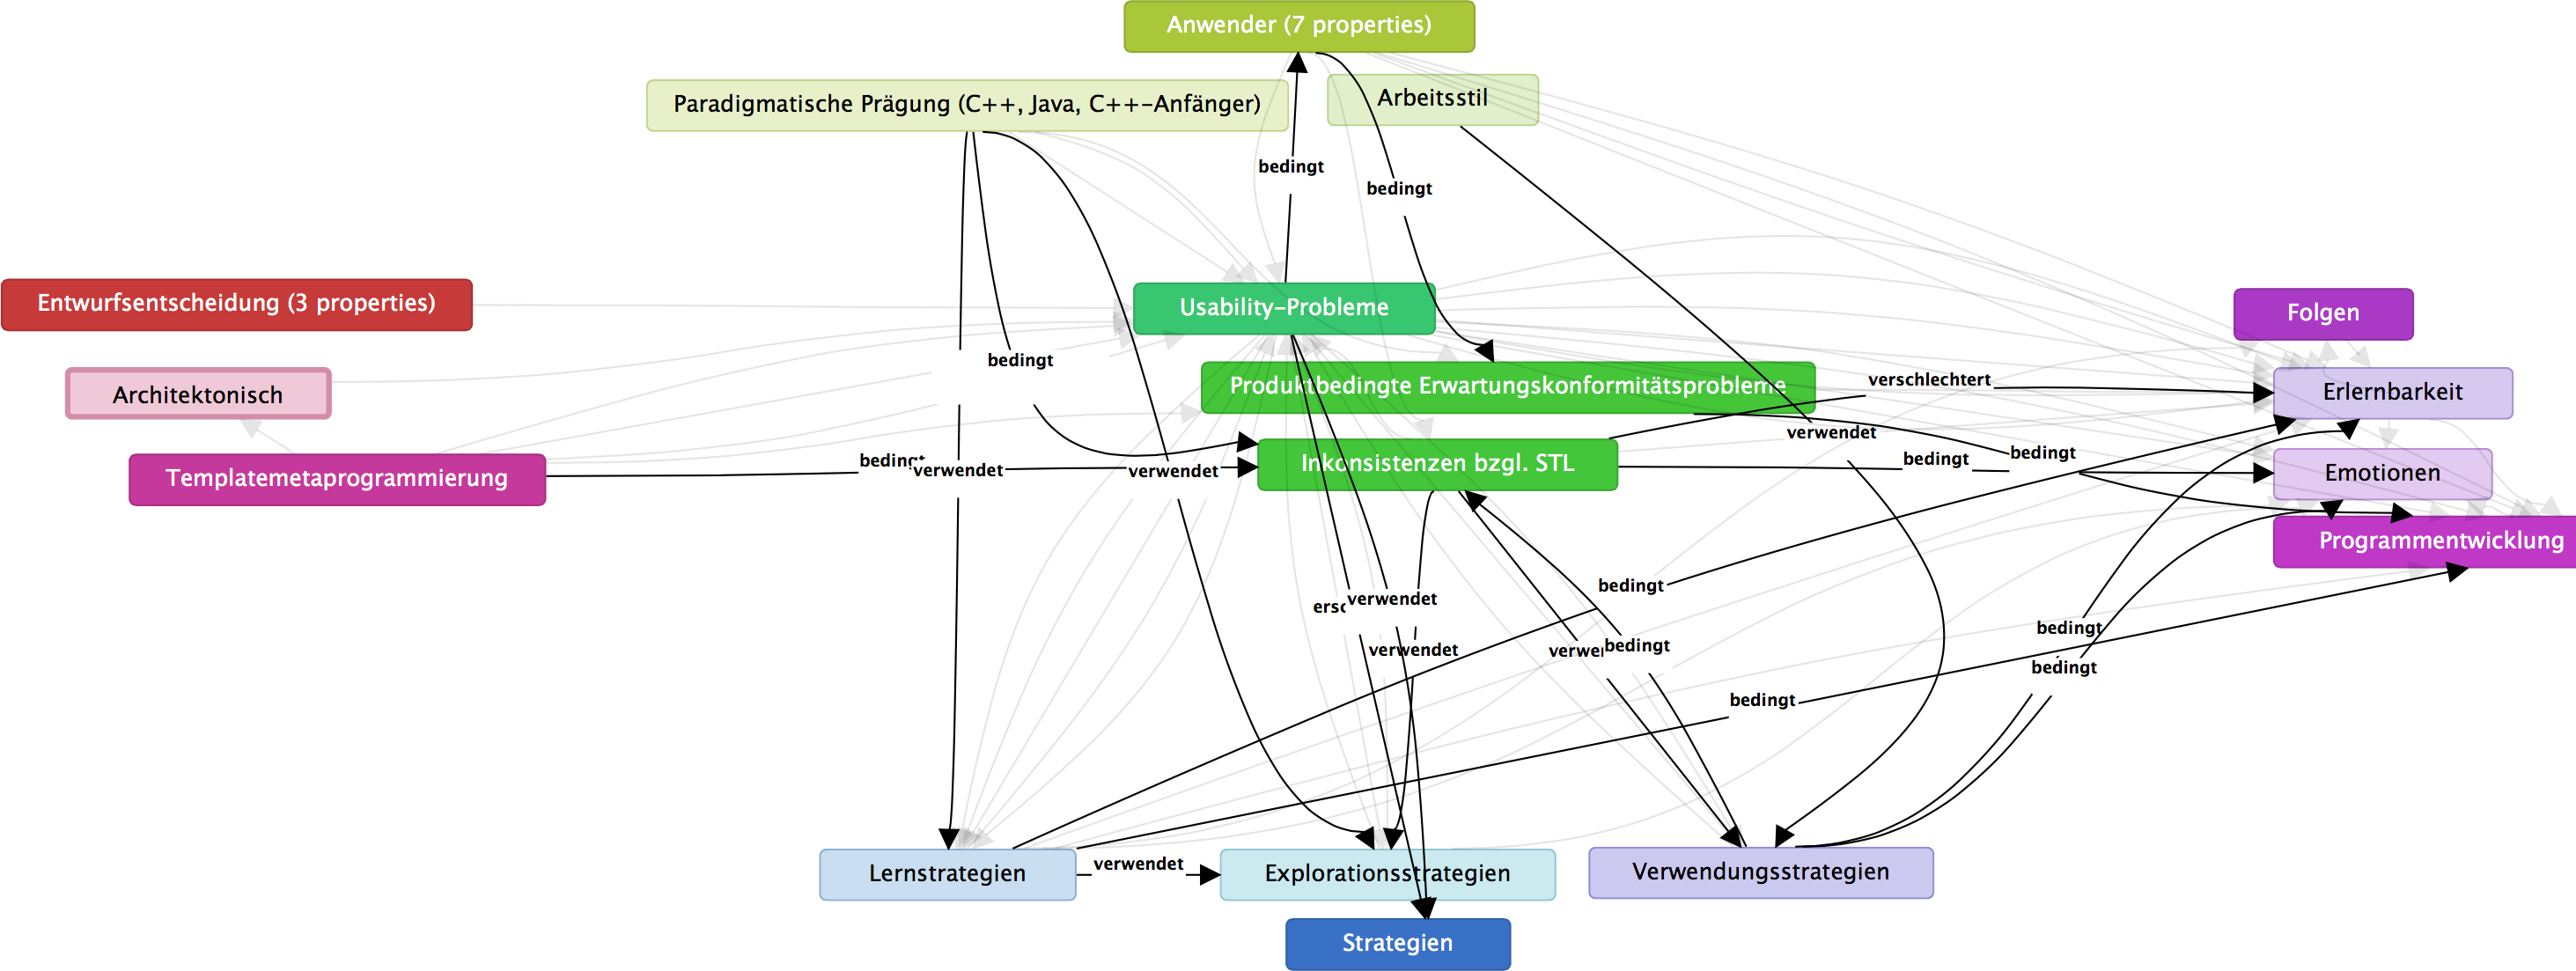
\includegraphics[width=1.0\linewidth]{Figures/research/gt-stl.png}
  \caption{Ursachen und Folgen des Problems \code{apiua://code/-9223372036854775633}}
  \label{fig:research-gt-stl}
\end{minipage}
\end{figure}


\subsubsection{Weiterer Vorschlag: Wrapper-API}
\label{sec:seqan-improve-wrapper-api}

Während ich die Umsetzung des CRTP-Vorschlags mit großer Überzeugung vertreten kann, fehlen mir für den folgenden Vorschlag hinreichend empirisch belegte Erkenntnisse --- siehe \code{apiua://code/-9223372036854775080} bzw. \textit{Java-objektorientierte} \code[apiua://code/-9223372036854775494]{paradigmatische Prägung}.

In der API-Usability-Evaluationsstudie von \cite{Stylos:2008cu} haben die Autoren festgestellt, dass ein Teil der Anwender API-Endanwender sind. Da diese Gruppe andere Anforderungen an eine API stellt, haben sich die Autoren dazu entschlossen, die existierende API nicht zu überarbeiten und damit womöglich die API-Usability für die technischen API-Anwender zu verschlechtern. Stattdessen haben sie eine auf der existierenden API aufbauende Wrapper-API geschaffen, die sich dadurch auszeichnet, dass sie API-Endanwender-zentrisch entwickelt wurde. Sie verfügt über ein weitaus höheres Abstraktionsniveau und verringert die Konfrontation mit technischen Belangen wie Thread-Sicherheit. Auf diese Weise verfügt die verbesserte Library nun über zwei aufeinander aufbauende APIs --- eine für API-Anwender und eine für API-Endanwender.

Dasselbe tat der Workshop'14-Teilnehmer John Reid im Zuge einer Arbeit \citep{Reid:R1ZT4-2v}, bei der SeqAn eingesetzt wurde. Auf Grund Reids großer Unzufriedenheit mit SeqAn\citepurl{bibtex://Reid:R1ZT4-2v}, implementierte er einen Python-basierten SeqAn-API-Wrapper mit Hilfe der \textit{Boost.Python}-Library\footnote{\url{http://www.boost.org/libs/python/}}. Dieser aufwändige Schritt unterstreicht zugleich die Fatalität der dazugehörigen Usability-Probleme. Der Wrapper sieht in seiner Anwendung wie folgt aus:
\begin{minted}[linenos=false]{python}
# Create a set of strings
seqs = seqan.StringDNASet(('ACGT', 'AAAA', 'GGGG', 'AC'))

# Create an enhanced suffix array
index = seqan.IndexStringDNASetESA(seqs)

# Traverse the array (DFS)
it = index.topdownhistory()
it.goBegin()
while not it.atEnd:
  print it.numOccurrences, it.representative
  it.goNext()
\end{minted}

Bereits bei dem ersten SeqAn-Workshop im Jahre 2011 äußerten einzelne Workshop-Teilnehmer im Rahmen der Feedback-Runde den Wunsch, SeqAn in ihre Python-Projekte verwenden zu können. Dieser Wunsch wurde jedoch schnell von Teilen der anwesenden SeqAn-Entwickler wegdiskutiert und nicht weiter verfolgt.

Die Arbeit von \cite{Stylos:2008cu} zeigt, dass es durchaus Sinn machen kann, verschiedene APIs für verschiedene Anwendergruppen zu implementieren. \cite{Reid:R1ZT4-2v} zeigte wiederum, dass eine zweite API möglich ist und wie sie objektorientiert aussehen kann, ohne Performanceverluste zu erleiden.

Erst spät wurde mir klar, dass der VIP-Förderantrag selbst eine solche Wrapper-API vorsah --- ohne sie als solches zu benennen. Die Rede ist von der Workflow-Engine KNIME, auf die ich bereits in den Abschnitten \ref{sec:rahmenbedingungen} und \ref{sec:argument-parser} eingegangen bin. KNIME erlaubt es, als visuelle Knoten gekapselte Programme grafisch zu verknüpfen und auf diese Weise Workflows zu erstellen (siehe \fref{fig:knime}). Eines der Ziele des ebenfalls im \sref{sec:rahmenbedingungen} vorgestellten BioStore-Projekts bestand in der Bereitstellung von SeqAn-Anwendungen innerhalb von KNIME. Es handelt sich dabei also um ein vom BioStore-Projekt erklärtes Ziel, das ich nun auf der Grundlage meiner Forschungsergebnisse unterstütze, weil es sich dabei um eine grafische Wrapper-API handelt, die sich besonders gut für API-Endanwender eignet \citep[vgl.][]{Ko:2004fc,Ko:2011el}. 

\begin{figure}
  \centering
    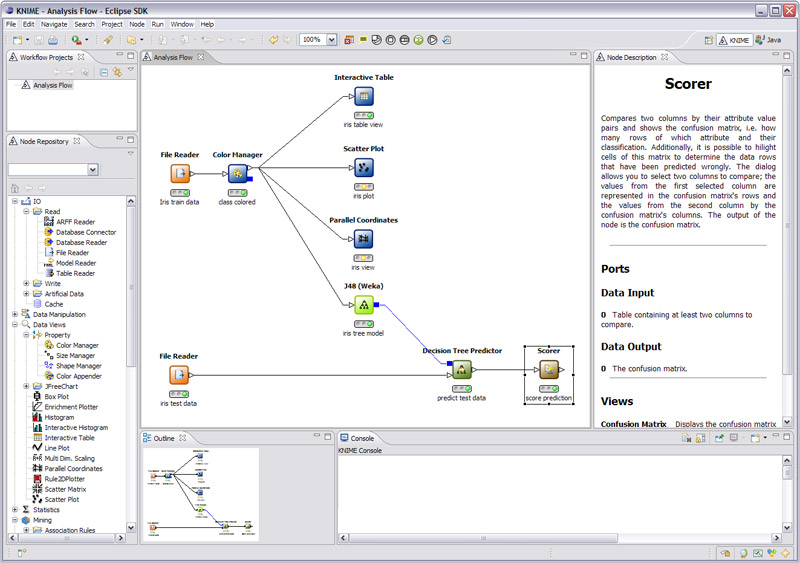
\includegraphics[width=0.8\linewidth]{Figures/knime.jpg}
  \caption{Workflow-Engine KNIME}
  \label{fig:knime}
\end{figure}




\subsection{Maßnahme: Intransparenzbeseitigung}
\textbf{Nutzen:} gering\footnote{Nur ein Anwender schilderte dieses Problem --- allerdings mit Vehemenz. Ich kann daher den genauen Nutzen nicht beurteilen.}; \textbf{Kosten:} mittel

Der Problem der \code[apiua://code/-9223372036854775057]{versteckten Parameterübergabe} muss durch eine explizite Parameterübergabe gelöst werden, was ich an dem folgenden Beispiel verdeutlichen möchte:

\begin{minted}[linenos=false,autogobble=false]{cpp}
typedef Index<DnaString, IndexQGram<UngappedShape<3> > > TIndex;
TIndex index("CATGATTACATA");
hash(indexShape(index), "CAT");
for (unsigned i = 0; i < length(getOccurrences(index, indexShape(index))); ++i)
  std::cout << getOccurrences(index, indexShape(index))[i] << std::endl; 
return 0;
\end{minted}

Dieses Beispiel könnte verbessert lauten:
\begin{minted}[linenos=false,autogobble=false]{cpp}
typedef Index<DnaString, IndexQGram<UngappedShape<3> > > TIndex;
TIndex index("CATGATTACATA");
TShape shape = indexShape(index);
THash shapeHash = hash(shape, "CAT");
for (unsigned i = 0; i < length(getOccurrences(index, shape, shapeHash)); ++i)
  std::cout << getOccurrences(index, indexShape(index))[i] << std::endl; 
return 0;
\end{minted}

In diesem Beispiel habe ich die Rückgaben der Funktionen \texttt{indexShape} und \texttt{hash} expliziert.

Da ich nur durch einen Proband auf dieses Problem aufmerksam wurde, dieses Thema in der API-Usability-Forschung nach meiner Kenntnis unerforscht ist und ich mich mit zeitlichen Problemen konfrontiert sah, habe ich diese Maßnahme nicht weiter verfolgt. Das mit dieser Maßnahme adressierte Problem \code[apiua://code/-9223372036854775057]{versteckte Parameterübergabe} ist jedoch Teil meines Ausblicks.




\subsection{Maßnahme: Inkonsistenzbeseitigung}
\textbf{Nutzen:} hoch; \textbf{Kosten:} hoch

\begin{itemize}
  \item \textit{Indirekte} \code[apiua://code/-9223372036854774918]{Datenstrukturmodifikationen} wie \mintinline{cpp}{fn(x) = 1} und \mintinline{cpp}{fn(fm(x), 1)} müssen durch \textit{direkte-explizite} Datenstrukturmodifikationen wie \mintinline{cpp}{x = 1} oder \mintinline{cpp}{x = fn(y)} ersetzt werden. \textit{Direkte-implizite} Datenstrukturmodifikationen wie \mintinline{cpp}{fn(x, 1)} sind tolerabel, wenn der Funktionsname auf eine Datenstrukturveränderung hinweist (z.B. \mintinline{cpp}{assignValue(x, 1)}).
  
  Auf diese Weise kann das Problem \code{apiua://code/-9223372036854775116} gelöst werden.
  
  \item Zusätzlich müssen Funktionen --- wenn kein dringender Grund dagegen spricht --- Referenzen zurückgeben und der Zuweisungsoperator entsprechend überschrieben werden, um das Problem der \code{apiua://code/-9223372036854774846} zu beheben.
  
%  \item \code{apiua://code/-9223372036854775533}: Wenn schon Shortcuts, dann konsistent (\mintinline{cpp}{String<AminoAcid>} => \mintinline{cpp}{AminoAcidString}) Get/Set nur theoretisch gesehen. Auswirkungen auf Usability-Probleme nicht weiter verfolgt. Daher keine Aussagen.

  \item In SeqAn werden Termini aus verschiedenen Domänen verwendet. Rein fachliche Termini wie \textit{Peptide} dürfen nur dann verwendet werden, wenn tatsächlich eine domänenentsprechende Kapselung mit Mehrwert zur benannten Datenstruktur zu Grunde liegt. Damit wird die Fatalität der Probleme \code{apiua://code/-9223372036854774861} und \code{apiua://code/-9223372036854775623} verringert.
\end{itemize}









\subsection{Maßnahme: Shortcuts}
\textbf{Nutzen:} mittel; \textbf{Kosten:} gering

\code{apiua://code/-9223372036854775611} sind ein Quell der Unmut und haben einen zweifelhaften Nutzen.

\begin{itemize}
  \item Der Name eines Shortcuts sollte sich aus den Bestandteilen ergeben, die es synonymisiert. Damit wird die Wahrscheinlichkeit verringert, dass Shortcuts eine \code[apiua://code/-9223372036854774861]{Abstraktion suggerieren}.
%  \item Der Name eines Shortcuts muss sich auf konsistente Weise ergeben, um einen Aspekt der \code{apiua://code/-9223372036854775533} zu beseitigen.
  \item Offensichtliche Shortcuts sollten entfernt werden oder zumindest nicht in für API-Anwender sichtbaren Code --- insbesondere Code-Beispielen --- verwendet werden. Dadurch kann das Problem \code{apiua://code/-9223372036854774860} gelöst werden.
\end{itemize}









\subsection{Maßnahme: Fail-Fast}
\textbf{Nutzen:} mittel; \textbf{Kosten:} gering

Die \code{apiua://code/-9223372036854775615} hat zwei Ursachen und muss daher auch auf zweierlei Weise gelöst werden:
\begin{enumerate}
  \item Globale (Meta-)Funktionen, die tatsächlich Interface-(Meta-)Funktionen sind, müssen auch als solche implementiert werden. Standardimplementierungen, die auch für ungeeignete Eingaben Werte zurückgeben, müssen beseitigt werden (z.B. \texttt{length}).
  \item Leseoperationen müssen die Möglichkeit zur Verfügung stellen, Lesefehler in Erfahrung zu bringen. Da Performance ein wichtiges Entwurfsziel von SeqAn ist, schlage ich vor, standardmäßig eine Verifikation der eingelesenen Daten vorzunehmen. Anwendern, die nicht bereit sind, diesen Performanceverlust hinzunehmen, muss die Möglichkeit gegeben werden, diese Verifikation zu deaktivieren (z.B. mit Hilfe von \texttt{Tags}).
  
  Ich schlage vor, eine Ausnahme im Falle eines Lesefehlers zu werfen. Der SeqAn-Core-Entwickler Manuel Holtgrewe begrüßte diesen Vorschlag bereits. 
\end{enumerate}


\subsection{Maßnahme: Dokumentation}\label{sec:dox}
\textbf{Nutzen:} hoch; \textbf{Kosten:} hoch

\code{apiua://code/-9223372036854775404} haben neben den \code{apiua://code/-9223372036854775633} die höchste Gesamtfatalität.

Die Dokumentation muss sowohl inhaltlich, als auch technisch überarbeitet werden.

\subsubsection{Inhaltliche Überarbeitung}

\paragraph{Gesamtüberblick}

Die SeqAn-Dokumentation leidet unter ihrem \code[apiua://code/-9223372036854775572]{fehlenden Gesamtüberblick}. Ein solcher muss daher bereitgestellt werden. Er muss folgendes umfassen:
\begin{itemize}
  \item Funktionale Abgrenzung: Was bietet SeqAn an Funktionen an und was nicht?
  \item Entwurf: Wie ``tickt'' SeqAn? Dieser Punkt könnte durch eine Gegenüberstellung eines typischen SeqAn-Programms mit anderen Sprachen erreicht werden. Für die Gegenüberstellung empfehle ich zwei hypothetische, semantisch identische Programme in Java-OOP und ``klassischem'' objektorientierten C\texttt{++}. Beispielsweise könnte die SeqAn-Programmzeile \mintinline{cpp}{resize(score, length(text) - length(pattern) + 1);} in Java \mintinline{java}{score.resize(text.length() - pattern.length() + 1);} lauten. Sobald die Maßnahme \textit{STL-Angleichung} umgesetzt ist, könnte der Vergleich zu C\texttt{++}/STL hinfällig sein.
  \item Entwurfsmotivation: Woher kommen die Unterschiede der Gegenüberstellung? Dieser Abschnitt muss die Motivation des Entwurfs --- beispielsweise durch einen Benchmark --- erläutern, um die Bereitschaft der Anwender zu erhöhen, sich weiterhin mit SeqAn zu befassen und eine höhere Toleranz für SeqAns Entwurf aufzubringen.
\end{itemize}

Eine ausführliche, aber nicht ausschweifende Erläuterung der grundlegenden Entwurfsentscheidungen unterstützt die \code[apiua://code/-9223372036854774821]{Lernstrategie} \code[apiua://code/-9223372036854775163]{konzeptionelles Verstehen}.
    
\paragraph{Beispiele}
\code{apiua://code/-9223372036854775581} behindern eine ganze Reihe von \code[apiua://code/-9223372036854774819]{Explorations-}, \code[apiua://code/-9223372036854774821]{Lern-}, und \code{apiua://code/-9223372036854774820}, was neben meiner Forschung auch die Arbeiten von \cite{Rosson:1996da,Stylos:2006td} für API-Anwender und von \cite{Wiedenbeck:kt,Rosson:2005hw} für API-Endanwender zeigen konnten.

Daher müssen alle nicht-trivialen Dokumentationseinträge über didaktische Code-Beispiele verfügen. Die Code-Beispiele müssen vollständig und voll funktionstüchtig sein, um es Anwendern zu erlauben, die Code-Beispiele ohne Anpassungen ausführen und besser verstehen zu können \citep{Rosson:1996da,Robillard:2010bh}.

\paragraph{Sprachentitätstypen} sind im Kontext von SeqAn ein wichtiges Konzept (siehe \sref{sec:gt-let}, Seite \pageref{sec:gt-let}), da SeqAn wegen seiner \code{apiua://code/-9223372036854775515} eine Fülle neuer \code{apiua://code/-9223372036854775413} einführt, die für SeqAns Anwender auf Grund derer \code[apiua://code/-9223372036854775494]{paradigmatischer Prägungen} unbekannt sind.

Daher schlage ich vor, Sprachentitätstypen explizit in der Dokumentation zu benennen und sämtliche Dokumentationseinträge mit ihrem jeweiligen Sprachentitätstyp zu annotieren. Eine separate Seite soll darüber hinaus alle in SeqAn verwendeten Sprachentitätstypen erläutern.

\paragraph{Punktuelle Verbesserungen}
Zur Lösung des Problems \code{apiua://code/-9223372036854775567} müssen die Unterschiede und Gemeinsamkeiten zwischen ähnlich benannten Typen (z.B. \texttt{String<String>} und \texttt{StringSet}) deutlich erklärt werden.

Eine weiteres Problem ist die \code[apiua://code/-9223372036854775577]{fehlende Dokumentation von Rückgabetypen}. Die Lösung liegt auf der Hand: Jede Erläuterung einer Funktionsrückgabe muss den zurückgegebenen Typ oder die zur Berechnung des Typs notwendige Metafunktion nennen. Damit wird auch gleichzeitig das Problem \code{apiua://code/-9223372036854775513} abgeschwächt.


\subsubsection{Technische Überarbeitung}

\paragraph{Auflistung sämtlicher Funktionen}
Die Dokumentation muss auf Grund der Usability-Probleme \code{apiua://code/-9223372036854775544} und \code{apiua://code/-9223372036854775280} und zur Unterstützung der \code{apiua://code/-9223372036854774819} \code{apiua://code/-9223372036854774900} unter jeder Klasse sämtliche zur Verfügung stehende Member-Funktionen, Interface-Funktionen und Member-Metafunktionen aufführen und klar voneinander unterscheiden. Um den Wartungsaufwand für die Dokumentation zu begrenzen, sollten sich die strukturellen Informationen aus den im Code manifesten Template-Spezialisierungen herleiten.

\paragraph{Suche}
Die \code{apiua://code/-9223372036854775504} innerhalb der Dokumentation muss so angepasst werden, dass sie die Suchergebnisse gewichtet sortiert und auf der Grundlage von Sprachentitätstypen gruppiert.

Das durch das \textit{Vocabulary Problem} bedingte Usability-Problem \code{apiua://code/-9223372036854775623} soll durch die Einführung von Aliassen gelöst werden. So muss beispielsweise der Suchbegriff \texttt{substring} den Dokumentationseintrag \texttt{infix} zu Tage fördern.

Wichtig an dieser Stelle ist die Unterscheidung zwischen den von mir vorgeschlagenen Aliassen und den als problematisch diagnostizierten Shortcuts. Während Shortcuts als eigenständige Entität dokumentiert sind und auch während der Programmierung alternativ genutzt werden können, dienen Aliasse lediglich dazu, unterschiedliche Suchbegriffe für einen bestimmten Dokumentationseintrag zu ermöglichen. Aliasse sind also weder eigenständig dokumentiert, noch können diese in Programmcode verwendet werden. Vielmehr erhöhen sie die Wahrscheinlichkeit eines erfolgreichen Suchtreffers und vermitteln dabei zugleich die in SeqAn verwendete Terminologie.

\paragraph{Fehlerfreiheit}

Die in der Dokumentation und in den \code{apiua://code/-9223372036854775271} verwendeten Code-Beispiele müssen defektfrei sein und kompilieren. Dazu müssen die Beispiele einer Quelle entspringen, die im Sinne der kontinuierlichen Integration (engl. \textit{continuous integration}) getestet wird.



\subsection{Maßnahme: Werkzeugunterstützung}
\textbf{Nutzen:} mittel; \textbf{Kosten:} mittel

Schaut man sich die in \sref{sec:api-tools} vorgestellten API-Werkzeuge an, muss man leider feststellen, dass keines der Arbeiten den Prototypen-Status je verlassen hat oder zumindest nicht als schlüsselfertiges Produkt vorliegt.

Eine Klasse von Werkzeugen unterstützt API-(End-)Anwender bei der Suche von Beispielen. Leider sind alle mir bekannten Lösungen, mit einer Emacs-Ausnahme, als Eclipse-Plugins implementiert. Des Weiteren haben sich die meisten Werkzeuge auf die Programmiersprache Java konzentriert.

Fasst man die Unreife der Werkzeuge, deren IDE- und Sprachabhängigkeit zusammen, muss man leider zu dem Schluss kommen, dass die Kosten für deren Anpassung, ihren Nutzen vermutlich übersteigen.

Die einzige Ausnahme bildet ein Algorithmus von \cite{Buse:2012vv}, der das Problem \code{apiua://code/-9223372036854775581} stark abmildern könnte. Dieser Algorithmus generiert automatisch Code-Beispiele für APIs, die auf typisierten Programmiersprachen basieren. Die Qualität der generierten Code-Beispiele wurde empirisch validiert. Ich halte es für sinnvoll, sich mit diesem Algorithmus näher zu beschäftigen und zu prüfen, mit welchen Kosten eine Anpassung an die Templatemetaprogrammierung-basierte generische Programmierung in C\texttt{++} möglich ist.



\subsection{Maßnahme: Kollaborationsplattform}
\textbf{Nutzen:} mittel; \textbf{Kosten:} mittel

Kollaborationsplattformen wie Webforen haben sich als nützliche Möglichkeit herausgestellt, eine andauernde Kommunikation zwischen API-Entwicklern und -Anwendern zu ermöglichen. Sie stellen eine exzellente Ressource für die Themen Debugging, Bugs und Entwurfsfragen dar. \citep{DaqingHou:2005ba}

Darüber hinaus bergen Webforen das Potential, API-Endanwendern das Wissen und die Hilfe von erfahrenen API-Anwendern zugänglich zu machen. \citep{Ko:2005cl}

Damit handelt es sich um eine relativ global wirkende Maßnahme, die sich dann positiv auf die \code{apiua://code/-9223372036854774824} von SeqAn auswirken sollte, wenn (1) dem Anwender das Problem bekannt ist und (2) der Anwender die Konsultation von Foren nicht scheut. 

Aus diesen Gründen schlage ich die Einrichtung einer Kollaborationsplattform vor.





\subsection{Probleme ohne Lösung}

\code{apiua://code/-9223372036854775100} können nach meiner Kenntnis leider nicht verbessert werden, sondern höchstens durch die Maßnahme \textit{Fail-Fast} verringert werden. Für API-Endanwender käme theoretisch das Debugging-Interface \textit{Whyline} \citep{Ko:2004fc} in Frage. Praktisch scheitert dieser Vorschlag jedoch an der Unreife dieser Lösung und der extrem hohen Kosten für die Anpassung an SeqAn (vgl. \sref{sec:api-tools}). Nur die Aufnahme von \textit{Concepts} in einen der kommenden C\texttt{++}-Sprachstandards könnte nach meiner Einschätzung Abhilfe schaffen.
        
Die \code{apiua://code/-9223372036854775279} besteht darin, dass mindestens zwei Funktionen, die den gleichen Namen tragen, unterschiedliche Dinge tun. Nach \cite{Bloch:2006jk} sollten solche Funktionen unterschiedliche Namen tragen. Dieser Empfehlung stimmen auch SeqAn-Anwender zu. Ungünstigerweise ist die Verwendung generischer --- und damit häufig gleich lautender Namen --- ja gerade das Grundprinzip der \code[apiua://code/-9223372036854775579]{generischen Programmierung}. Würde man die Funktion \texttt{calc} auftrennen in \texttt{calcA} und \texttt{calcB} würde man die \textit{Erweiterbarkeit} einer API massiv beeinträchtigen. Dieses Problem kann also lediglich durch Aufklärung in der Dokumentation teilweise gelöst werden.

Das von mir während meiner Heuristischen Evaluation gefundene Problem der \textit{fehlenden IDE-Integration der Dokumentation} ist der Tatsache geschuldet, dass das aktuelle \textit{DDDoc}-Dokumentationsformat von SeqAn nicht mit dem Dokumentationssystem \textit{Doxygen}\footnote{Es handelt sich dabei um das C\texttt{++}-Pendant zu JavaDoc. Siehe \url{www.doxygen.org}} kompatibel ist. SeqAn hat besondere Anforderungen an das Dokumentationsformat, da es die in SeqAn verwendeten \textit{Concepts} abbilden muss, die noch nicht in den aktuellen C\texttt{++}-Sprachstandard aufgenommen wurden. Jedoch schlage ich unter der Maßnahme Dokumentation eine Änderung des aktuellen Dokumentationsformats vor, die Doxygen ähnelt. Sobald Concepts in den C\texttt{++}-Sprachstandard aufgenommen wurden, sind sehr wahrscheinlich nur noch kleine Anpassungen notwendig, um die Dokumentation in die IDE des Anwenders integrieren zu können.

Die \code[apiua://code/-9223372036854775148]{fehlende Autovervollständigung} ist der \code{apiua://code/-9223372036854775396} von \code[apiua://code/-9223372036854775579]{generischer Programmierung} durch Entwicklungsumgebungen geschuldet. Es ist davon auszugehen, dass die Aufnahme von Concepts in den C\texttt{++}-Sprachstandard zu einer besseren Autovervollständigung führen werden. Diese Entwicklung würde auch den Strategien \code{apiua://code/-9223372036854775145} und \code{apiua://code/-9223372036854774900} entgegen kommen.



\subsection{Weitere Maßnahme: Usability-Priorisierung}
\textbf{Nutzen:} hoch; \textbf{Kosten:} \textit{mittel}

Wie ich bereits im \sref{sec:gt-urursache} angesprochen habe, befindet sich SeqAn gerade dabei, sein Einsatzgebiet auf den kommerziellen Bereich auszuweiten. Diese Entwicklung gibt der zuvor vernachlässigten Usability einen neuen Stellenwert.

SeqAn-Entwickler müssen bei zukünftigen Entwicklungen, wie der Unterstützung von GPUs\footnote{Grafikprozessor ---\textit{Graphics Processing Unit}} und der Parallelisierung von Algorithmen, nun nicht mehr nur Performance und Funktionalität, sondern auch Usability \textit{gleichwertig} miteinander vereinbaren und ihre wissenschaftliche Arbeitsweise ebenfalls auf die Usability übertragen (Stichwort: Usability-Engineering).

Dafür gibt es zwei Gründe:
\begin{enumerate}
  \item Durch die Verwendung eines Consultance-Vermarktungsmodells stehen SeqAn-Entwickler im direkten Kontakt zu ihren Kunden. \textit{Technisches Wegargumentieren} wäre für die Kommunikation mit den Kunden schädlich \citep{Sarodnick:2006vc}.
  \item SeqAn ist zwar eine der schnellsten, aber nicht die einzige Bioinformatik-Softwarebibliothek auf dem Markt. Eine hohe Performance kann eine schlechte Usability nur in Maßen aufwiegen. Tut sie das nicht, wechseln die Kunden zu einem anderen Produkt \citep{sunshine2014searching}. Dies belegen auch meine erhobenen Daten\citepurl{apiua://survey/cd/2013-09-19T11:51:16.616+02:00/provisionality}.  
\end{enumerate}  




\subsection{Zusammenfassung}

In diesem Unterkapitel habe ich Vorschläge zur Verbesserung der API-Usability von SeqAn auf der Grundlage meiner zuvor erhobenen Usability-Probleme und Strategien unterbreitet. Diese Vorschläge sind in Bezug auf die Usability-Probleme weitgehend disjunkt. Die meisten Maßnahmen lassen sich daher hinreichend isoliert bearbeiten.

Die Entwurfsentscheidungen \code{apiua://code/-9223372036854775515} und \code[apiua://code/-9223372036854775579]{generische Programmierung} machen Gebrauch von \textit{Concepts} --- also Interface-ähnlichen Typ-Anforderungsbeschreibungen --- notwendig, von denen SeqAn bereits Gebrauch macht. Allerdings ist in diesem Punkt SeqAn seiner Zeit voraus, denn Concepts sind bis heute nicht in den C\texttt{++}-Sprachstandard aufgenommen worden. Erst C\texttt{++}17 wird voraussichtlich Concepts in die Sprache aufnehmen \citep{Schmidt:2014tf}.

Nach Aufnahme von Concepts in C\texttt{++} ist kurzfristig damit zu rechnen, dass \code{apiua://code/-9223372036854775396} wie die \code[apiua://code/-9223372036854775148]{fehlende Autovervollständigung} und die \code{fehlende IDE-Integration der Dokumentation} entfallen werden. Ich rechne außerdem damit, dass die Lesbarkeit von \code{apiua://code/-9223372036854775100} zunehmen wird, da durch die Unterstützung von Concepts eine Reihe von bisher nur in SeqAn verwendeten \code{apiua://code/-9223372036854775413} auch im Compiler als solche benannt werden.

Mittelfristig rechne ich damit, dass sich die durch Concepts eingeführten neuen \code{apiua://code/-9223372036854775413}, wie \textit{Interface-Funktionen}, innerhalb der C\texttt{++} geprägten Anwenderschaft etablieren werden. Zwar profitieren C\texttt{++} unerfahrene, aber Java-erfahrene Anwender weniger davon, diese werden jedoch bereits durch die Beseitigung der \code{apiua://code/-9223372036854775396} unterstützt.

Die Aufnahme von Concepts in den C\texttt{++}-Sprachstandard bilden also nur einen Baustein bei der Verbesserung der API-Usability von SeqAn.

Die vier wichtigsten Usability-Verbesserungsmaßnahmen sind \begin{itemize}
\itemsep1pt\parskip0pt\parsep0pt
  \item SeqAns Umstellung von einem Framework auf eine Library,
  \item SeqAns Angleichung an die STL,
  \item die Implementierung einer speziell für API-Endanwender entwickelten Wrapper-API und
  \item die Verbesserung der Dokumentation.
\end{itemize}

Ergänzt werden diese Maßnahmen durch punktuellere Maßnahmen wie der Überarbeitung von Shortcuts sowie der Beseitigung von Intransparenzen, Inkonsistenzen und Versagensverschleppungen.

Abschließend habe ich vorgeschlagen, den Dokumentationsaufwand zu begrenzen. Dazu empfiehlt es sich, bereits im Code vorhandene strukturelle Informationen für die Generierung der Dokumentation zu nutzen, das Dokumentationsformat \texttt{DDDoc} syntaktisch zu vereinfachen und den Code-Beispiel-Generationsalgorithmus von \cite{Buse:2012vv} zu evaluieren.

\bigskip

Das nächste Unterkapitel befasst sich mit den bereits erreichten API-Usability-Verbesserungen von SeqAn.

\section{Verbesserung der API-Usability von SeqAn}
\label{sec:seqan-api-usability-verbesserung}

Dieses Unterkapitel behandelt die erreichten API-Usability-Verbesserungen an Hand der im vorherigen Unterkapitel vorgeschlagenen Maßnahmen und wiederholt in sehr knapper Form die bereits in Phase 1 erläuterten Verbesserungen im Zuge der ersten Beseitigung grober Usability-Probleme.

Auf Grund der im gleichnamigen \hyperref[sec:schwierigkeiten]{Abschnitt erläuterten Schwierigkeiten} (S. \pageref{sec:schwierigkeiten}) konnte ich nicht für die Umsetzung aller Maßnahmen sorgen. Ganz besonders sind dabei, neben organisatorischen Gründen wie dem Wegfall von Kollegen und meiner auf drei Jahre begrenzten Stelle, wissenschaftliche Gründe, wie den Anwendungsschwierigkeiten der \gls{gtm} und dem unerwartet aufwändigen Analysewerkzeugbau, zu nennen. Aus den damit einhergehenden zeitlichen Problemen musste ich auch die im nächsten Unterkapitel vorgestellte Validierung stark kürzen.

\subsection{Prozessverbesserungen}

Im Zuge der ersten Beseitigung grober Usability-Probleme habe ich in Zusammenarbeit mit der Bioinformatik-Arbeitsgruppe die folgenden Prozessverbesserungen vorgenommen, die sich wie folgt positiv auf die Usability auswirken:
\begin{itemize}
  \item Die Einführung standardisierter Commit-Nachrichten führte zu verständlicheren und ausführlicheren Beschreibungen der Entwicklungen an SeqAn. Dies half mir als API-Evaluator die Arbeiten an SeqAn besser nachvollziehen zu können. Augenscheinlich mag dieser Schritt unwichtig wirken. Durch die hohe Dynamik in meinem Arbeitsumfeld (insb. die vielen Akteure und die stetige Fortentwicklung von SeqAn; siehe \sref{sec:rahmenbedingungen}) war diese Verbesserung jedoch von großer Wichtigkeit für mich und wirkte sich positiv auf mein Arbeitsergebnis aus.
  \item Die Umstellung von Subversion auf Git verbesserte den Entwicklungsprozess für die SeqAn-Entwickler, da sie nun lokale Revisionen erstellen konnten, ohne das zentrale Repository zu kompromittieren. Dieser Zugewinn an Freiheitsgraden erhöht die \textit{sequenzielle Vollständigkeit} der Entwicklungs-\textit{Arbeitsaufgabe}\footnote{Hierbei handelt es sich um Begriffe aus der Arbeitspsychologie. ``Eine Handlung ist sequenziell vollständig, wenn in ihr der gesamte Handlungszyklus abgedeckt ist, d.h. es kommt sowohl zu Zielbildungs-, Planungs- und Ausführungsprozessen als auch zu Kontrollprozessen.'' \citep{Bamberg:2011tv}} und damit die Wahrscheinlichkeit einer höheren Softwarequalität. Ich gehe nicht davon aus, dass ein Zugewinn an Softwarequalität zu einer Verschlechterung der API-Usability führt --- eher im Gegenteil.
  \item Die Einführung von Code-Reviews als Instrument der Qualitätssicherung verbessert ebenfalls die Softwarequalität.
\end{itemize}

Weitere Details können im \sref{sec:phase1} nachgelesen werden.



\subsection{Frameworkumbau}

SeqAn wurde erfolgreich von einem Framework zu einer Library umgebaut. Die SeqAn-Entwickler haben sämtliche Vorwärtsdeklarationen beseitigt. Fortan ist es möglich, SeqAn sowohl als Framework als auch als Library zu verwenden. Für Letzteres gibt es eine eigene Anleitung, die in allen Installationsanleitungen verlinkt ist\footnote{\url{http://seqan.readthedocs.org/en/latest/BuildManual/IntegrationWithYourOwnBuildSystem.html}}.

In Folge gibt es nun auch keine Abhängigkeiten mehr zum CMake-Build-System, der Anwender dazu zwingen könnte, den eigenen Build-Prozess umzustellen.



\subsection{STL-Angleichung}

\subsubsection{Curiously Recurring Template Pattern --- CRTP}

Ich habe das CRTP einigen SeqAn-Entwicklern zu einer Zeit präsentiert, in der ich noch in dem Glauben war, SeqAns Anwender würden eine streng objektorientierte Library erwarten. Dies entsprach zum Einen nicht den Tatsachen, denn ein großer Teil erwartete lediglich eine STL-konforme Softwarebibliothek. Zum Anderen stieß ich mit diesem Vorschlag auf Ablehnung. Ich hatte den Eindruck, dass die Idee, die SeqAn-API zu einer reinen OOP-API umzustrukturieren, für die SeqAn-Entwickler ein zu radikaler Schritt wäre.

Aus zeitlichen Gründen kam ich nicht mehr dazu, dem SeqAn-Team meinen neuen Erkenntnisstand mitzuteilen.

Die in \sref{sec:stl-inconsistencies} beschriebenen Beobachtungen lassen erwarten, dass die Umwandlung von in SeqAn globalen Funktionen, die in C\texttt{++} als Memberfunktionen implementiert wären, eine äußerst positive Auswirkung auf die Usability haben wird.

\subsubsection{Metafunktionen}

Metafunktionen werden in der SeqAn-API vornehmlich zur Berechnung von Rückgabetypen verwendet, was --- obwohl Gogol-Döring damit eine Verbesserung der Usability beabsichtigte --- tatsächlich eine Verschlechterung selbiger (siehe \code{apiua://code/-9223372036854775352}-Problem) verursachte.

Dieser Anwendungsfall ist durch das \texttt{auto}-Schlüsselwort im neuen C\texttt{++}-Sprachstandard obsolet geworden, was auch die Dynamik meines Forschungsvorhabens unterstreicht (vgl. \sref{sec:schwierigkeiten}). Mittels \texttt{auto} wird der Compiler angewiesen, den Datentyp selbstständig herzuleiten. Auf diese Weise würde man statt \mintinline{cpp}{Row<Align<String<Dna>, ArrayGaps>>::Type &row1 = row(align, 0);} nur noch \mintinline{cpp}{auto &row1 = row(align, 0);} schreiben müssen.

\subsection{KNIME als API-Endanwender-Werkzeug}

Während die STL-Angleichung die bestehende SeqAn-API an die Erwartung von C\texttt{++}-geprägten API-Anwendern annähern soll, geht es bei der Wrapper-API darum, eine zweite, speziell auf die Bedürfnisse von API-Endanwendern angepasste API zu entwickeln. Die Bereitstellung von SeqAn-Programmen innerhalb der Workflow-Engine KNIME war eines der Ziele des BioStore-Projekts (siehe Abschnitte \ref{sec:rahmenbedingungen}). Dieses Ziel haben die Bioinformatik-Arbeitsgruppe und ich wie folgt erreicht:
\begin{enumerate}
  \item KNIME-Anpassungen
  \begin{enumerate}
    \item[1.] Das von der Universität Tübingen entwickelte \textit{Common Tool Description (CTD)} Format wurde weiterentwickelt und erlaubt nun eine mächtige Beschreibung der Schnittstelle von Kommandozeilenprogrammen. Beschreibungsmöglichkeiten umfassen u.a. typisierte Argumente und Wertebereiche (vgl. \sref{sec:argument-parser}).
    \item[2.] Das ebenfalls ursprünglich an der Universität Tübingen entwickelte \textit{Generic KNIME Nodes}, wurde unter dem Namen \textit{Generic Workflow Nodes}\footnote{\url{https://github.com/genericworkflownodes}} weiterentwickelt. Es kann, unter Verwendung von CTD-Dateien, die entsprechenden Kommandozeilenprogramme als KNIME-Knoten kapseln. Diese können dann über das Internet für alle KNIME-Anwender bereitgestellt werden.
  \end{enumerate}
  \item SeqAn-Anpassungen
  \begin{enumerate}
    \item[1.] Es wurde ein neuer Parser für Argumente implementiert (siehe \sref{sec:argument-parser}).
    \begin{itemize}
      \item Der Argument-Parser ist Bestandteil der SeqAn-API und bietet mächtige Funktionen zur Beschreibung von Kommandozeilenprogrammschnittstellen.
      \item Ein Argument-Parser verwendendes SeqAn-Programm kann seine eigene Schnittstellenbeschreibung als CTD-Datei exportieren.
      \item Sämtliche SeqAn-Anwendungen (siehe \sref{sec:seqan-tools}) wurden an den Argument-Parser angepasst und verwenden diesen nun.
    \end{itemize}
    \item[2.] Die kontinuierliche Integration (engl. \textit{continuous integration --- CI}) wurde angepasst.
    \begin{itemize}
      \item Der SeqAn-CI-Server generiert nun für alle SeqAn-Anwendungen CTD-Dateien.
      \item Die SeqAn-Anwendungen werden mit Hilfe der CTD-Dateien und der Generic Workflow Nodes Anwendung zu KNIME-Knoten gepackt.
      \item Die SeqAn-KNIME-Knoten\footnote{\url{https://tech.knime.org/seqan-nodes-for-knime}} werden auf den Community-Server von KNIME hochgeladen und stehen damit allen KNIME-Anwendern zu Verfügung\footnote{\url{http://seqan.readthedocs.org/en/master/HowTo/UseSeqAnNodesInKnime.html}}.
    \end{itemize}
    \item[3.] Analog zu SeqAn-Code-Beispielen, wurden beispielhafte Workflows entwickelt\footnote{\url{https://github.com/seqan/knime_seqan_workflows}}, die in KNIME importiert werden können.
  \end{enumerate}
\end{enumerate}

Die SeqAn-Anpassungen erlauben es darüber hinaus SeqAn-Anwendern KNIME-Knoten aus ihren selbst entwickelten SeqAn-Anwendungen zu generieren.\footnote{\url{http://seqan.readthedocs.org/en/latest/HowTo/GenerateSeqAnKnimeNodes.html}}

Das Ergebnis besteht darin, dass KNIME-Anwender nun grafisch mit SeqAn arbeiten können. Dazu können SeqAn-Anwendungen in Form von Knoten auf einer KNIME-Arbeitsfläche platziert, verbunden und konfiguriert werden (siehe Abbildungen \ref{fig:knime-example} und \ref{fig:knime-config}). Auf diese Weise können API-Endanwender SeqAn-Workflows entwickeln, ohne eine einzige Zeile Code schreiben zu müssen.

\begin{figure}
  \centering
    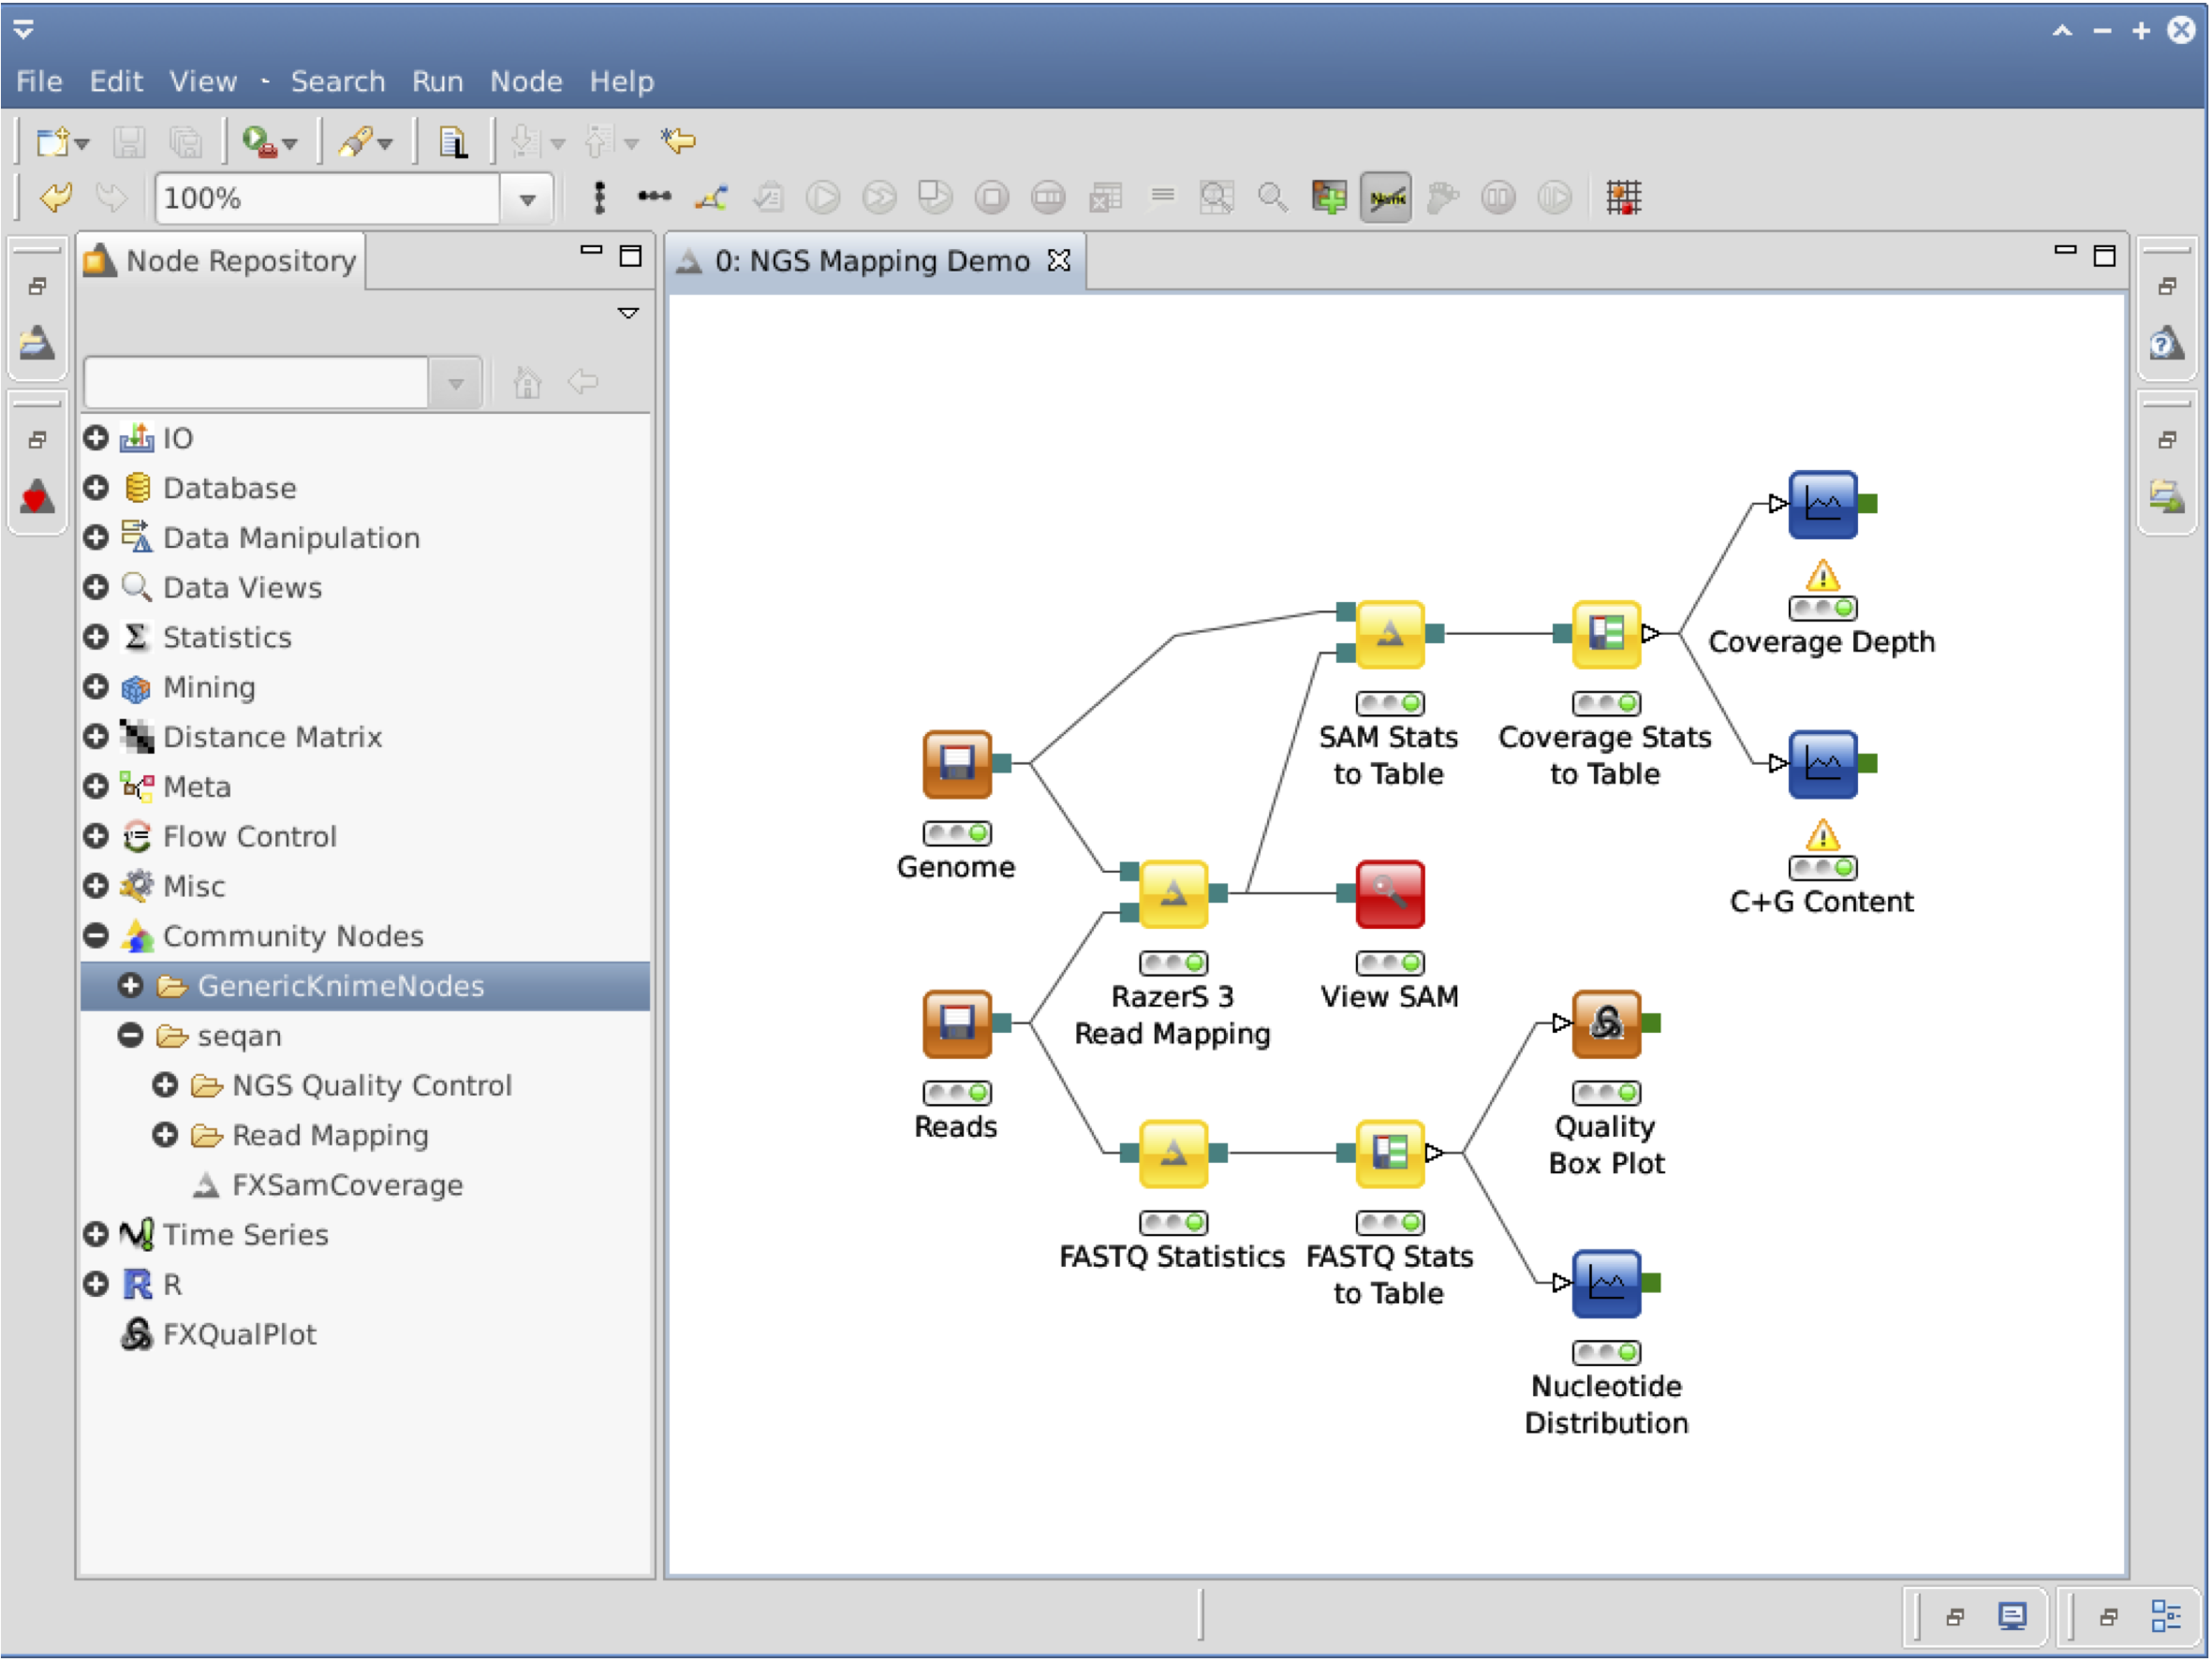
\includegraphics[width=1\linewidth]{Figures/knime-example.png}
  \caption{Beispiel-SeqAn-Workflow in KNIME}
  \label{fig:knime-example}
\end{figure}

\begin{figure}
  \centering
    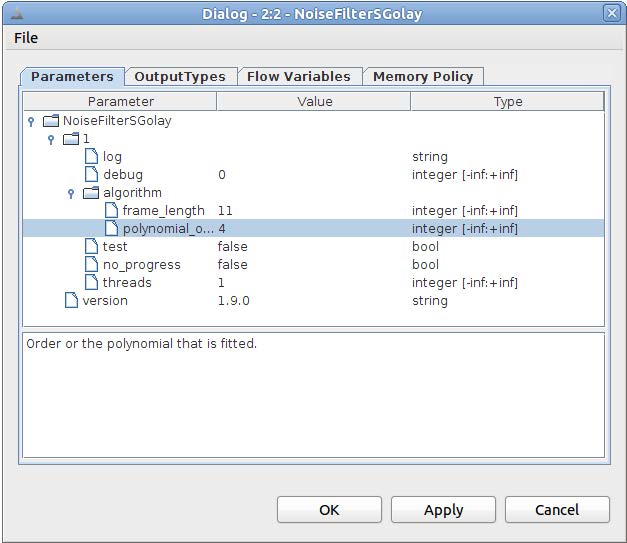
\includegraphics[width=0.65\linewidth]{Figures/knime-config.jpg}
  \caption{KNIME-Konfigurationsdialog für einen CTD-basierten Knoten}
  \label{fig:knime-config}
\end{figure}



\begin{comment}
\subsection{Intransparenzbeseitigung}

Die Fatalität des Problems der \code[apiua://code/-9223372036854775057]{versteckten Parameterübergabe} ist nicht hinreichend verstanden, um aktuell den SeqAn-Entwicklern die Problembeseitigung zu empfehlen.
\end{comment}


\subsection{Inkonsistenzbeseitigung}
\label{sec:Inkonsistenzbeseitigung}

Die Probleme \code{apiua://code/-9223372036854775116}, \code{apiua://code/-9223372036854774846} und \code{apiua://code/-9223372036854774861} wurden mit den SeqAn-Core-Entwicklern besprochen. Jedoch kam es nicht zu einer konkreten Planung zur Umsetzung dieser Maßnahme, was zwei Gründe hatte:
\begin{itemize}
  \item Zum Zeitpunkt der Vorstellung meiner Ergebnisse waren meine Lösungsvorschläge nicht konkret genug.
  \item Meine Kollegen verfolgten während der BioStore-Projektzeit genauso eigene Ziele, wie ich das mit der API-Usability-Erfoschung tat. Nach meiner Einschätzung des Standpunktes der SeqAn-Entwickler stand der Nutzen dieser Maßnahme in keinem guten Verhältnis zu den Kosten.
\end{itemize}



\subsection{Shortcuts}

Während des BioStore-Projekts, das vor einem knappen Jahr endete, konnte ich die Sensibilität für die mit den Shortcuts einhergehenden Probleme auf Seiten der SeqAn-Entwickler erhöhen. Jedoch waren meine damaligen Lösungsansätze nicht hinreichend fundiert, um die SeqAn-Entwickler zu einer Lösung der Probleme \code{apiua://code/-9223372036854774861} und \code{apiua://code/-9223372036854774860} zu bewegen.



\subsection{Fail-Fast}

Diese Maßnahme bestand aus zwei Schritten:
\begin{enumerate}
  \item Dass es Funktionen wie \texttt{length} gibt, die bei bestimmen Eingaben ungültige Rückgaben liefern, war einigen SeqAn-Entwicklern unabhängig von meinen Forschungsergebnissen bekannt. Der Entwickler Manuel Holtgrewe erachtete deren Korrektur ebenfalls für sinnvoll. Aktuell ist dieser Schritt noch nicht umgesetzt.
  \item Die Einschätzung, dass Leseoperationen Ausnahmen werfen müssen, wenn es zu einem Lesefehler kommt, teilten anfangs nur sehr wenige SeqAn-Entwickler aus Angst, SeqAn würde dadurch langsamer arbeiten. Die Notwendigkeit dieser Maßnahme und dessen Vereinbarkeit mit dem SeqAn-Entwurfsziel \textit{Performance} mittels \textit{Tags} fand zunehmend Zustimmung. Allerdings ging diese Maßnahme in den letzten Projektmonaten --- insbesondere aus Zeitgründen bei allen Beteiligten --- unter. Die Beseitigung steht also noch aus.
\end{enumerate}




\subsection{Dokumentation}
\label{sec:improve-dox}

Die SeqAn-Dokumentation besteht im weiteren Sinne aus den Installationsanleitungen, didaktischen Lernressourcen (Tutorials) und der Dokumentation selbst, die als Nachschlagewerk für SeqAn-Anwender dient.

Im Zuge der ersten Beseitigung grober Usability-Probleme habe ich gemeinsam mit meinen Kollegen bereits die Installationsanleitungen und die Tutorials umfassend überarbeitet. Die Wirksamkeit dieser Überarbeitungen habe ich bereits im \sref{sec:phase1-validierung} gezeigt. An dieser Stelle fasse ich diese Änderungen nur sehr knapp zusammen:


\subsubsection{Installationsanleitungen}

Die Installationsanleitungen waren fehlerhaft, uneinheitlich, unstrukturiert und verfügten über zu wenig Beispiele, um den Anleitungen folgen zu können. Ich habe eine inhaltliche und grafische Vorlage für alle plattformabhängigen Installationsanleitungen erstellt und dabei die folgenden Installationsanleitungsbestandteile etabliert:
\begin{enumerate}
\itemsep1pt\parskip0pt\parsep0pt
  \item Prerequisites --- Was bereits installiert sein muss + Verweise
  \item Install --- Die eigentliche SeqAn-Installation
  \item A First Build --- Überprüfung, ob Installation korrekt verlief
  \item Hello World! --- Skelett für erste eigene SeqAn-Anwendung
  \item Further Steps --- Verweise auf Dokumentation und Tutorials
\end{enumerate}

Sämtliche Installationsanleitungen wurden korrigiert und vereinheitlicht. \fref{fig:getting-started-windows2} zeigt einen Ausschnitt aus der Installationsanleitung für Windows.

\begin{figure}[ht!]
  \centering
    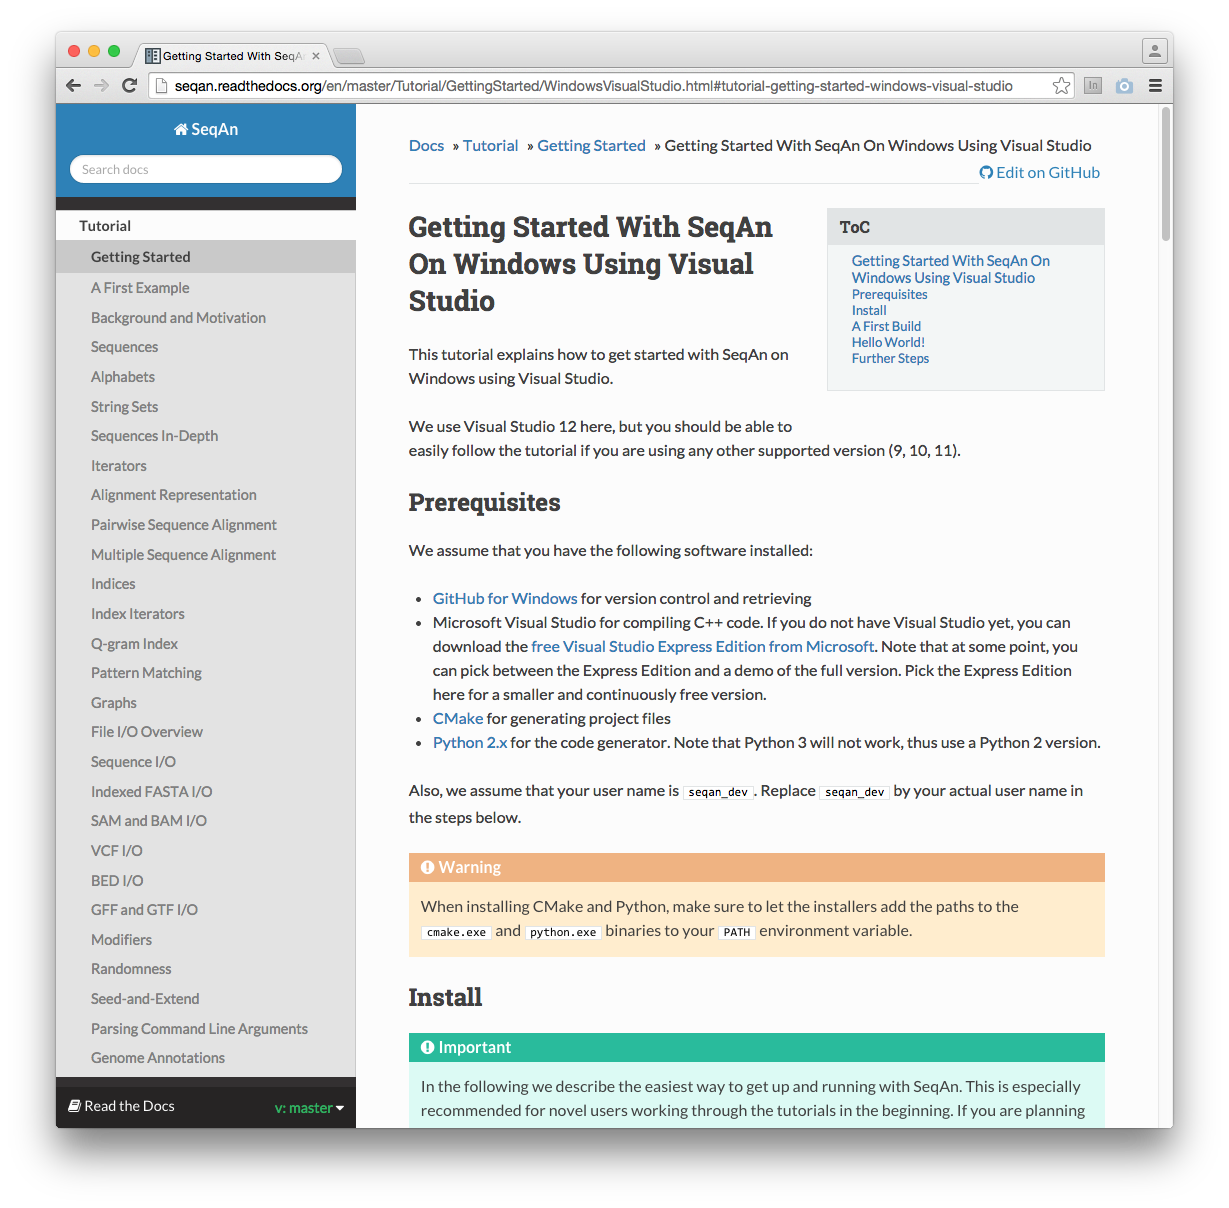
\includegraphics[width=1.0\linewidth]{Figures/getting-started-windows.png}
  \caption[SeqAn-Installation unter Windows]{Ausschnitt aus der verbesserten SeqAn-Installationsanleitung für Windows}
  \label{fig:getting-started-windows2}
\end{figure}



\subsubsection{Tutorials}

Basierend auf dem etablierten Lernphasenmodell \citep{Gagne:1985tx} und den Analyseergebnissen einer Vielzahl von Daten (Details siehe \sref{sec:phase1}) habe ich die Struktur der Tutorials überarbeitet und Qualitätskriterien formuliert. Diese Ergebnisse habe ich in Form eines Tutorials über das Schreiben von Tutorials zusammengefasst und in die Entwickler-Dokumentation integriert\footnote{\url{http://seqan.readthedocs.org/en/master/HowTo/WriteTutorials.html}}. Das Dokument richtet sich an die Autoren von SeqAn-Tutorials, wurde von diesen sehr positiv aufgenommen, gilt seitdem als verbindliche Vorlage für neue Tutorials und stellt damit einen langfristigen Beitrag für die verbesserte API-Usability von SeqAn dar.

Das Dokument besteht aus den folgenden Abschnitten:
\begin{enumerate}
\itemsep1pt\parskip0pt\parsep0pt
  \item Konventionen, die beim Verfassen von Tutorials zu beachten sind
  \item Struktur --- Aufbau eines Tutorials, explizite Metaangaben
  \item Didaktik --- Anwenderzentrierung, Übungsaufgaben
  \item Integration --- Vernetzung des Tutorials für bessere Auffindbarkeit
  \item Vorlage --- für die Erstellung eines neuen Tutorials
\end{enumerate}

Es wurden mehrere neue Tutorials durch das Auftrennen existierender Tutorials geschaffen. Besonders erwähnenswert ist dabei das neue Anfänger-Tutorial ``A First Example''\footnote{\url{http://seqan.readthedocs.org/en/master/Tutorial/FirstStepsInSeqAn.html}}, das eine besonders geringe Einstiegshürde für Anwender mit den in der \gls{gtm}-Analyse gefundenen \code[apiua://code/-9223372036854775494]{paradigmatischen Prägungen} aufweist. Es lohnt sich für den Leser dieser Dissertation das Anfänger-Tutorial einmal selbst zu öffnen.

Die Tutorials wurden sukzessive über eine längere Diskussionsphase hinweg gemeinsam von mir und den jeweiligen Autoren verbessert (siehe \fref{fig:tutorial-improved-final}) und dienen fortan als Aufgaben-bezogener SeqAn-Überblick \citep[vgl.][]{Fairbanks:2006jw,Ko:2011vw,Pugh:Ks4cicwp,Robillard:2009cs}.

\begin{figure}[ht!]
  \centering
    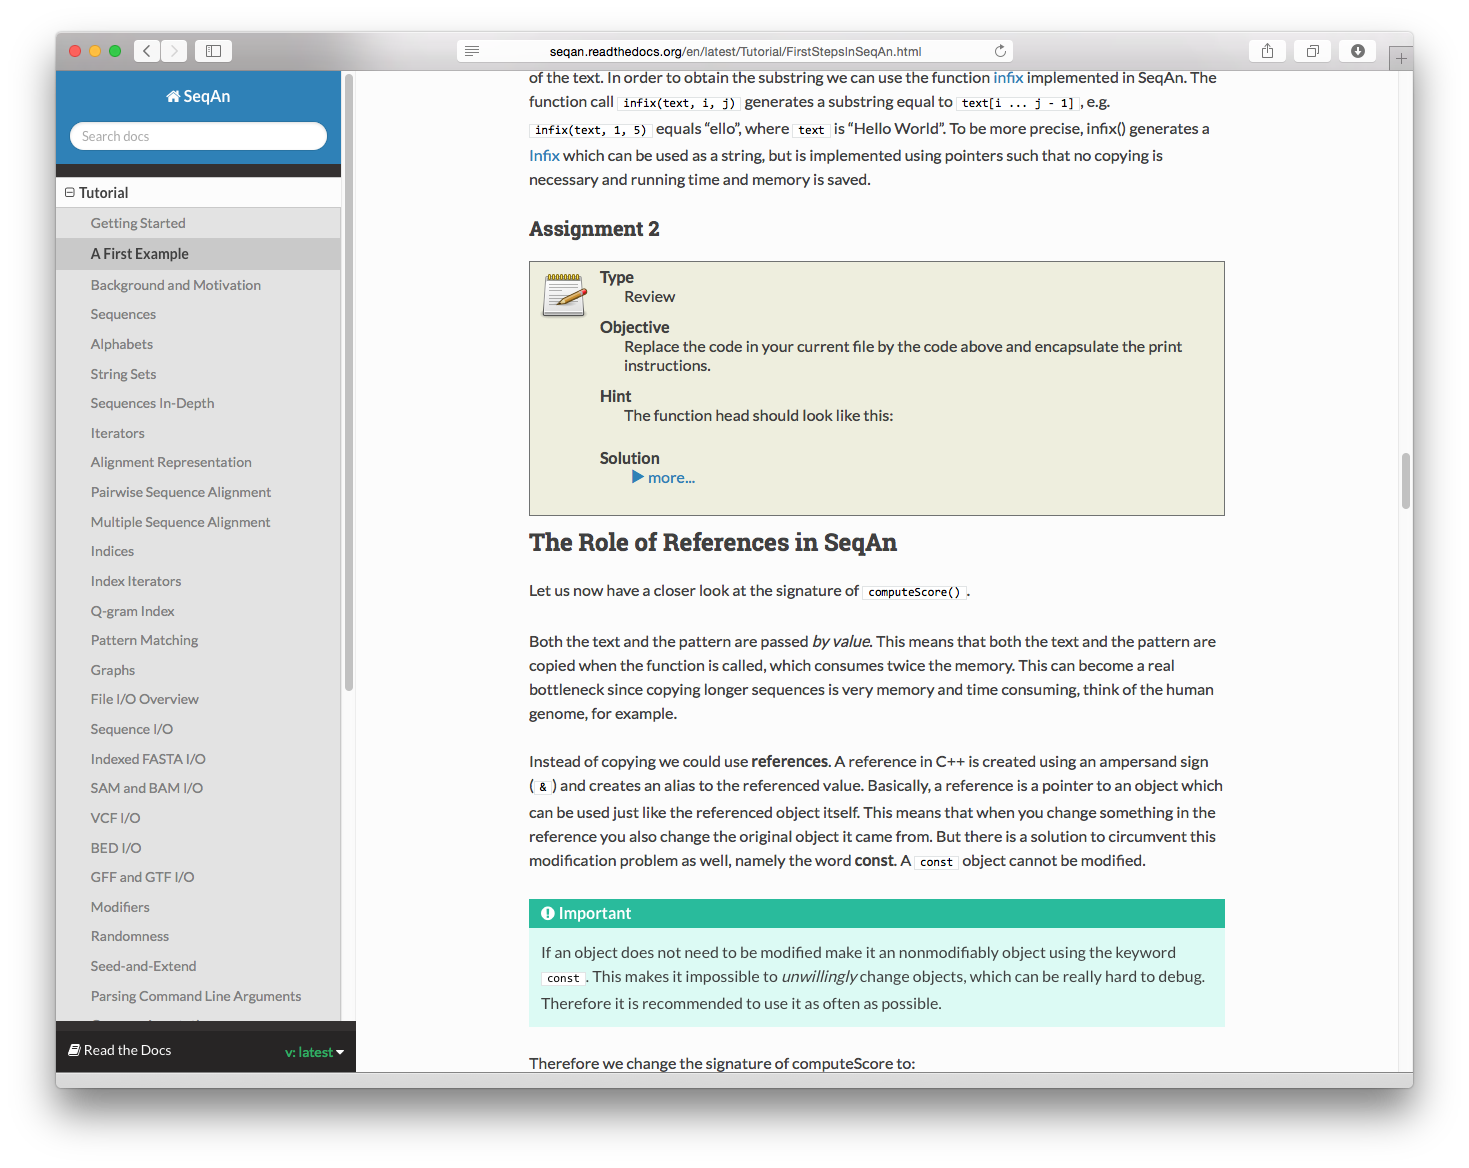
\includegraphics[width=1\linewidth]{Figures/tutorial-improved-final.png}
  \caption{Beispiel für ein überarbeitetes Tutorial}
  \label{fig:tutorial-improved-final}
\end{figure}




\subsubsection{Dokumentation}

Dokumentationen bilden ein wichtiges Bindeglied zwischen dem, was der Anwender möchte und dem, was die Library anbietet \citep{Robillard:2009cs,Kintsch:1988bz,Pennington:1987dc}. Aus diesem Grund und meinen \gls{gtm}-Analyseergebnissen habe ich die eigentliche SeqAn-Dokumentation technisch von Grund auf neu entwickelt. Die inhaltliche Überarbeitung wurde von den SeqAn-Entwicklern durchgeführt. Die \fref{fig:dox-large-all} zeigt die alte und die neue Dokumentation im Vergleich. Alternativ bietet es sich an, während des Lesens dieses Abschnitts die Dokumentation unter \href{http://docs.seqan.de/seqan/develop/}{docs.seqan.de/seqan/develop/} selbst zu öffnen.

Im Folgenden erläutere ich die Änderungen gegenüber der alten Dokumentation.

\newgeometry{inner=2cm,outer=1.5cm,top=1.5cm,bottom=1.5cm}
\thispagestyle{empty}
\begin{landscape}
\begin{figure}
        \centering
        \begin{subfigure}[b]{0.38\linewidth}
                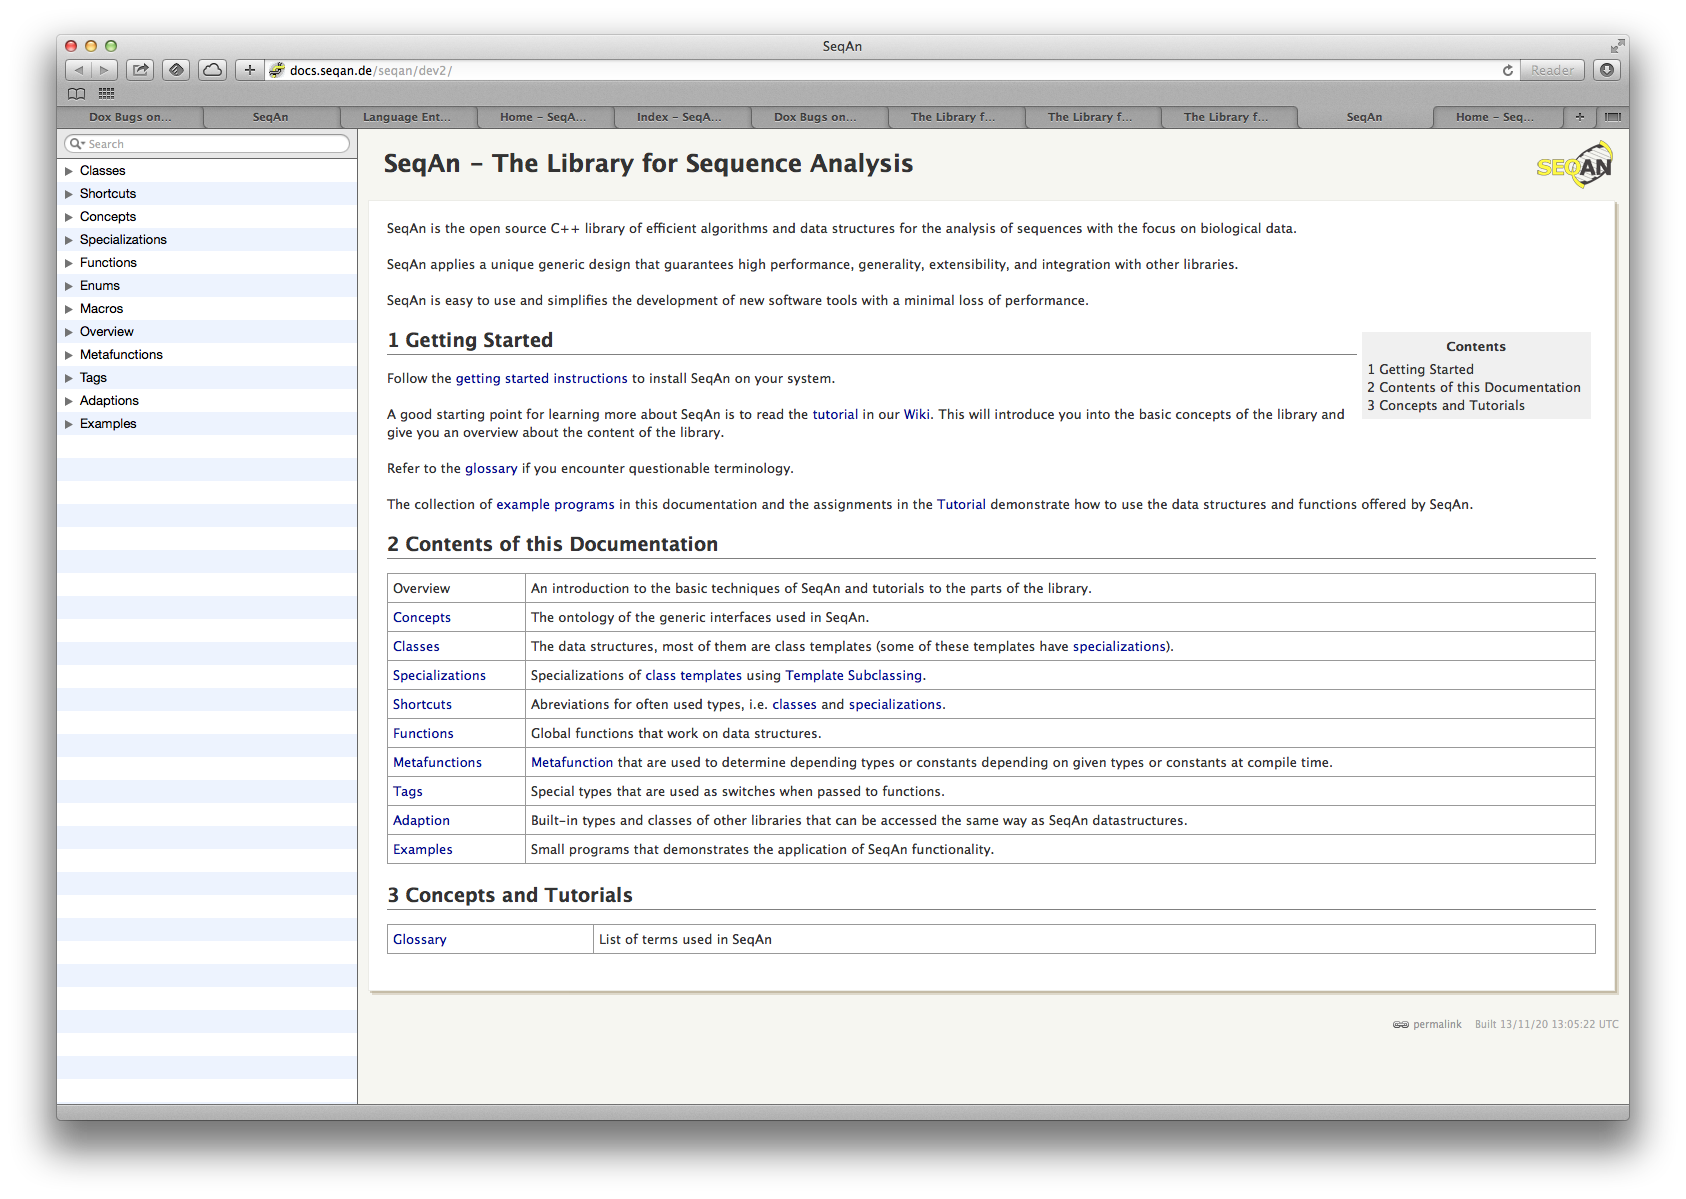
\includegraphics[width=\linewidth]{Figures/dox/dox-2_0_0-large-home.png}
                \caption{Startseite in Version 2.0.0}
                \label{fig:dox-large-home-2.0.0}
        \end{subfigure}
        \hspace{1cm}
        \begin{subfigure}[b]{0.38\linewidth}
                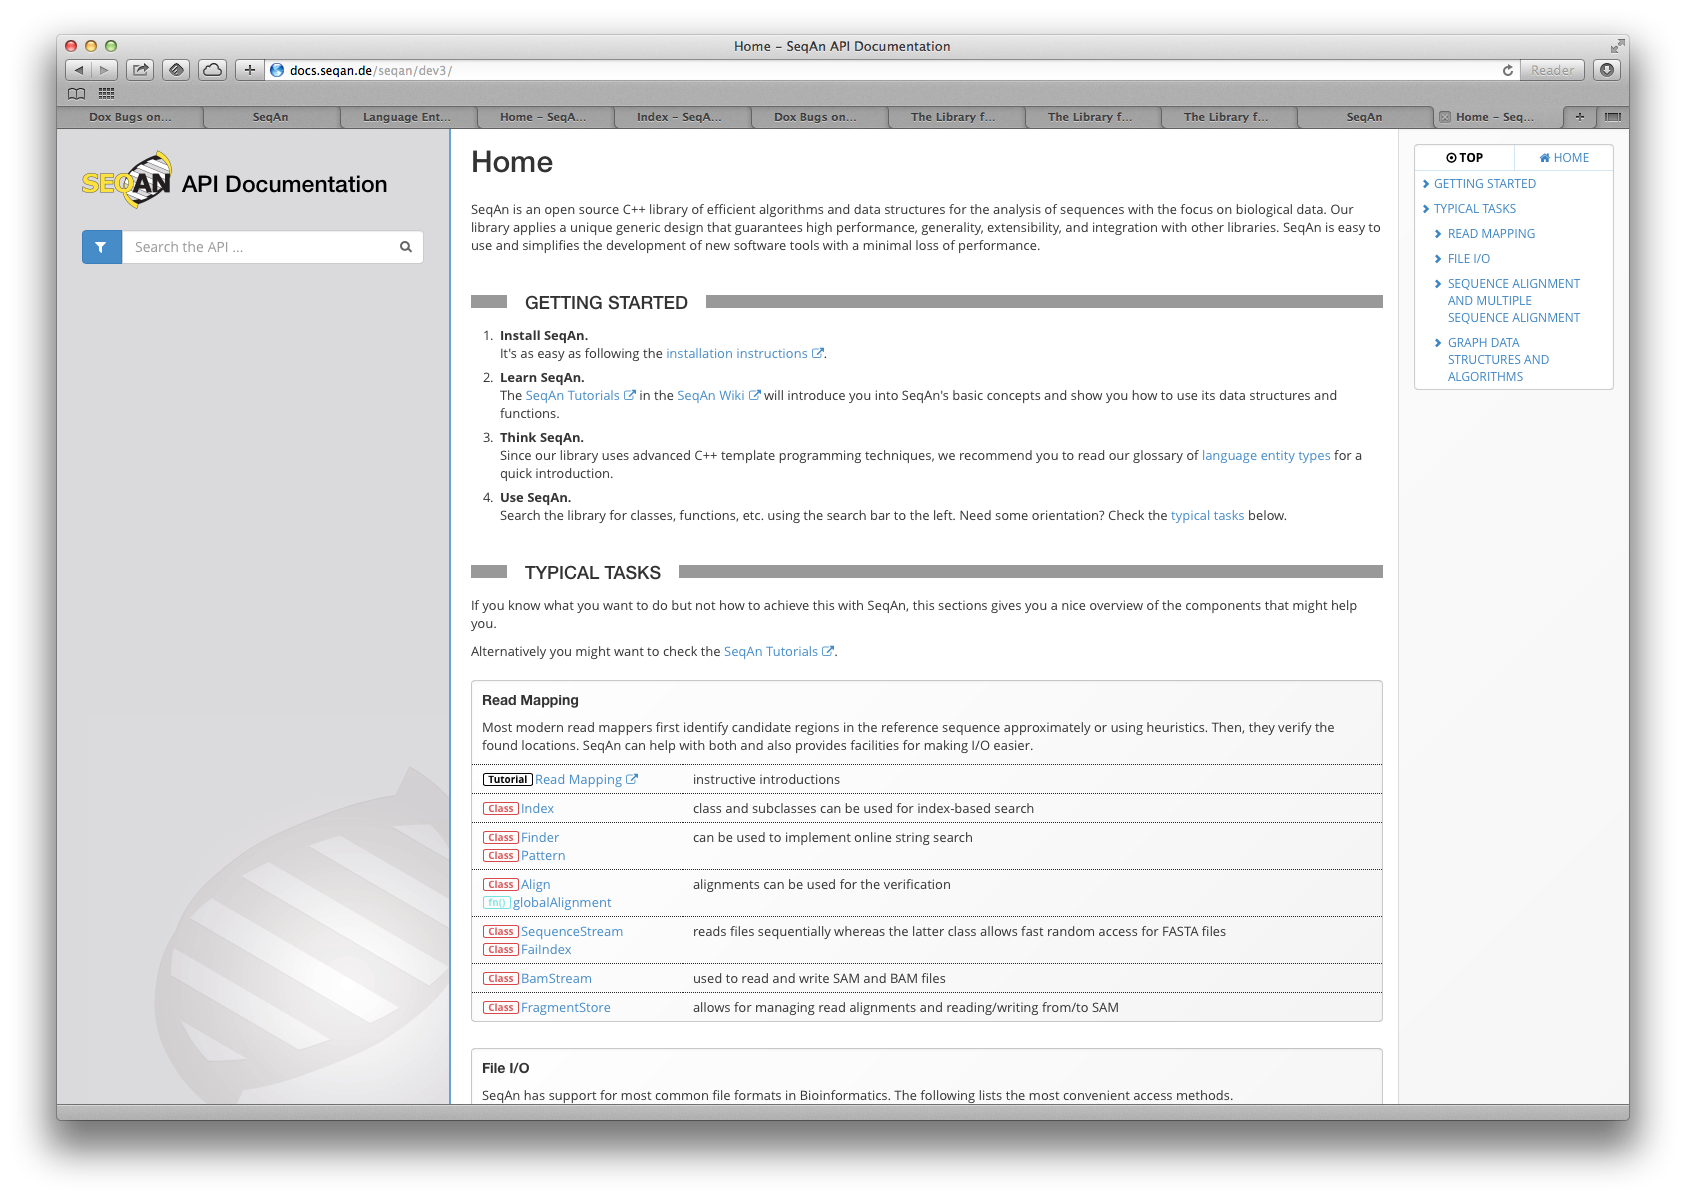
\includegraphics[width=\linewidth]{Figures/dox/dox-3_0_0-large-home.png}
                \caption{Startseite in Version 3.0.0}
                \label{fig:dox-large-home-3.0.0}
        \end{subfigure}%
        \vskip\baselineskip
        \begin{subfigure}[b]{0.38\linewidth}
                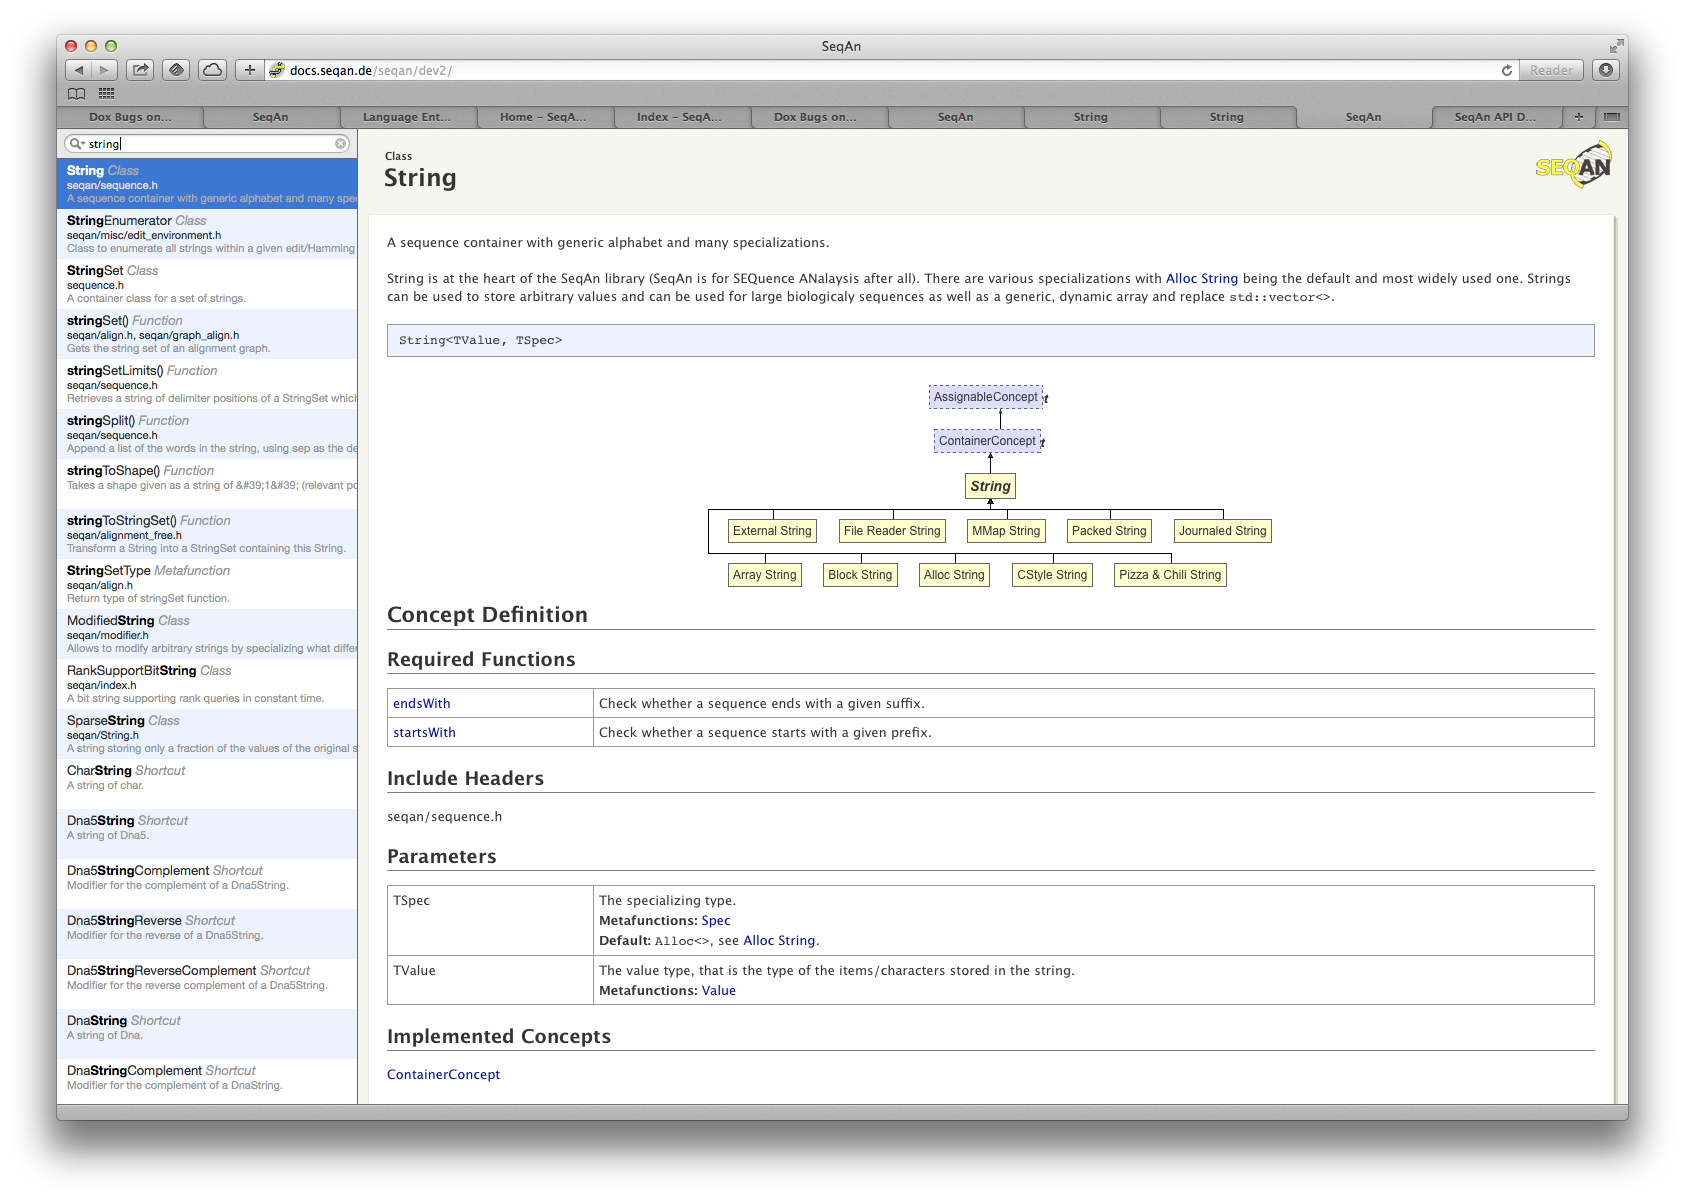
\includegraphics[width=\linewidth]{Figures/dox/dox-2_0_0-large-string-opened.png}
                \caption{Geöffnete \texttt{String}-Klasse in Version 2.0.0}
                \label{fig:dox-large-string-opened-2.0.0}
        \end{subfigure}
        \hspace{1cm}
        \begin{subfigure}[b]{0.38\linewidth}
                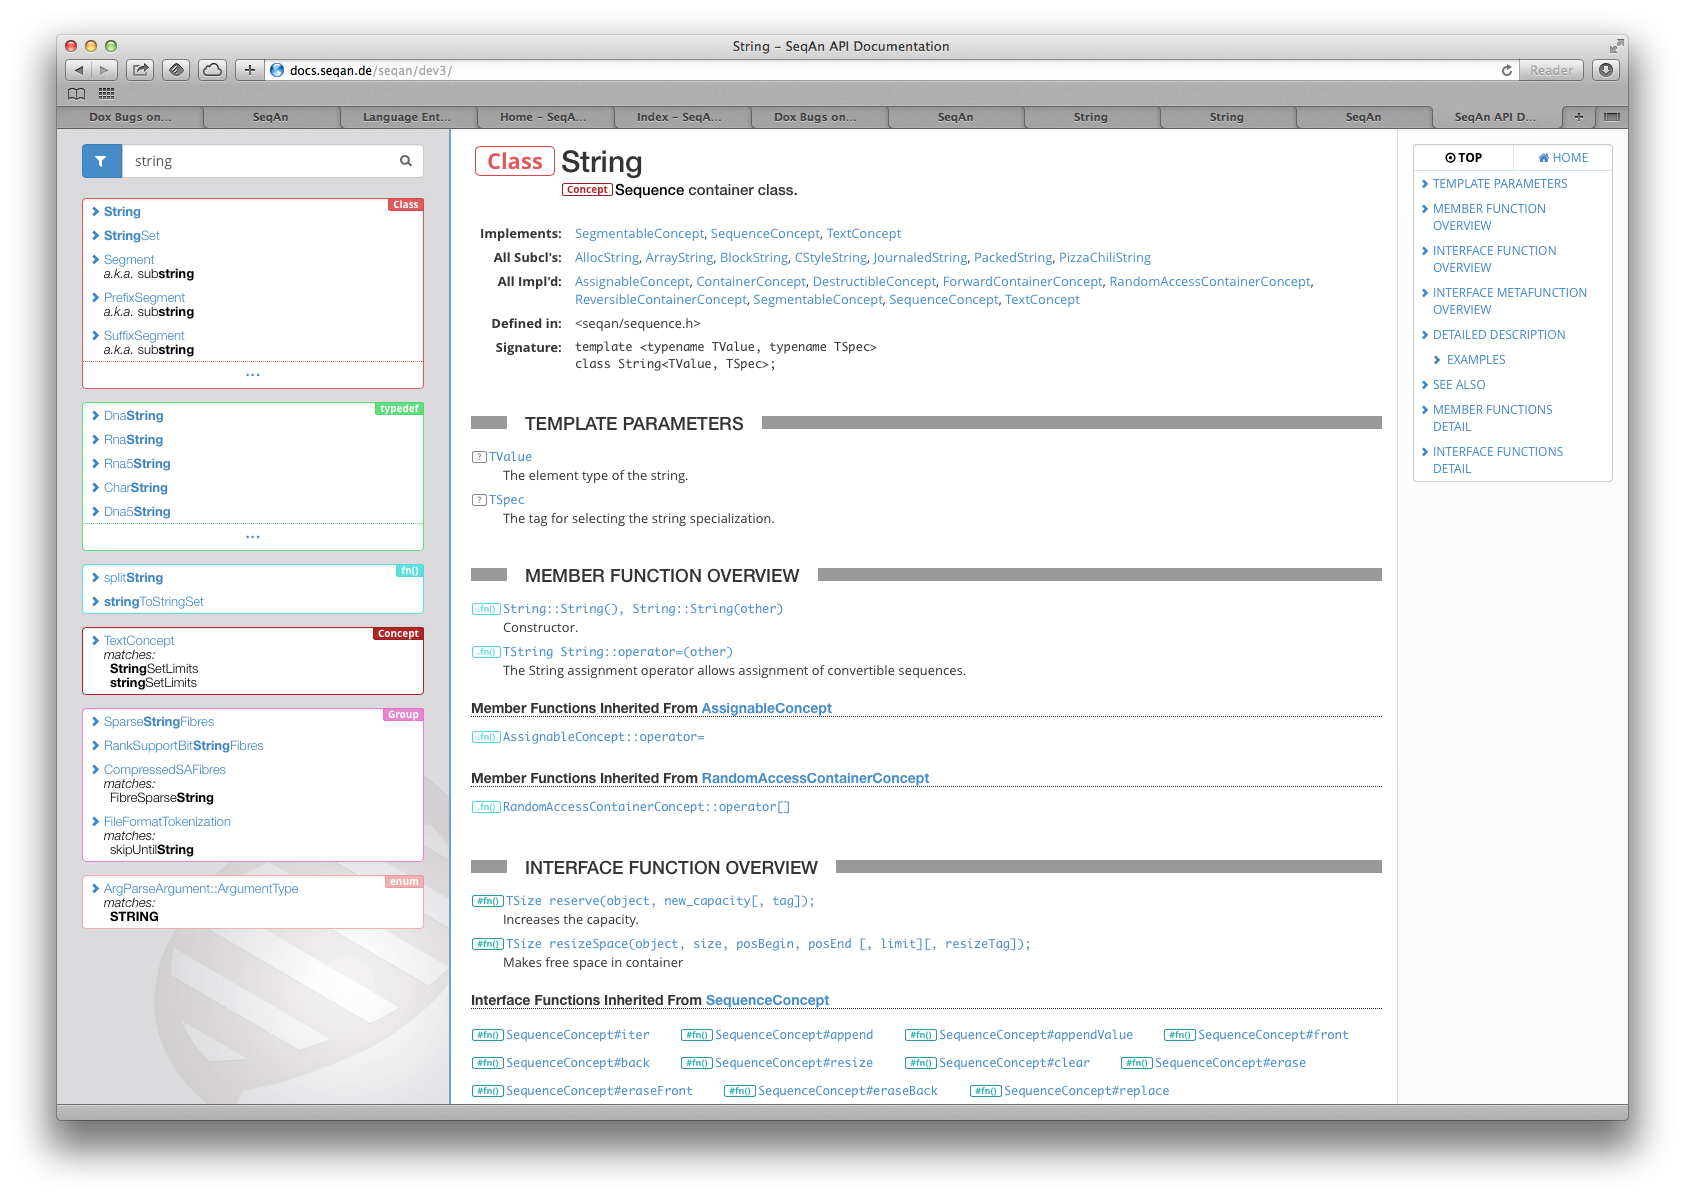
\includegraphics[width=\linewidth]{Figures/dox/dox-3_0_0-large-string-opened.png}
                \caption{Geöffnete \texttt{String}-Klasse in Version 3.0.0}
                \label{fig:dox-large-string-opened-3.0.0}
        \end{subfigure}
        \caption[Alte und neue Dokumentation im Vergleich --- in normaler Breite]{Die Abbildungen zeigen die alte und neue Dokumentation.}
        \label{fig:dox-large-all}
\end{figure}
\end{landscape}
\restoregeometry










\paragraph{Dokumentationssystem}

In Vorbereitung auf die technische Neuentwicklung der Dokumentation haben meine Kollegen und ich zunächst das in SeqAn verwendete Dokumentationssystem überarbeitet.

Der SeqAn-Entwickler Gogol Döring entwarf das \code[apiua://code/-9223372036854774817]{Dokumentationssystem} \textit{DDDoc} im Zuge einer \textit{expliziten-argumentativen} \code{apiua://code/-9223372036854775281}. Notwendig war (und ist) ein selbst entwickeltes Dokumentationssystem, da SeqAn, die noch nicht in den C\texttt{++}-Sprachstandard aufgenommene Sprachentität \textit{Concept} verwendet.\footnote{Gogol-Dörings Einschätzung, dass Concepts unbedingt Bestandteil der Dokumentation sein müssen, konnte ich empirisch bestätigen. Wie die Probleme \code{apiua://code/-9223372036854775280} und \code{apiua://code/-9223372036854775544} zeigen, können ohne Concepts die inhaltliche Zusammengehörigkeit technisch global implementierter \mbox{(Meta-)Funktionen} vom Anwender nicht erkannt werden. Tatsächlich handelt es sich nämlich bei den meisten globalen Funktionen inhaltlich um \mbox{Interface-(Meta-)Funktionen.}}

Wie das folgende kleine Beispiel zeigt, unterscheidet sich DDDoc von bekannten Dokumentationssystemen wie JavaDoc oder Doxygen, indem es ungewöhnlich zu lesen und zu schreiben ist.

\begin{center}
\begin{minted}[linenos=false, firstnumber=1]{cpp}
/**
.Spec.SimpleScore
..general:Class.Score
..summary:Basic scoring scheme.
..description:
This class allows to do alignments with simple match/mismatch-based scores.
..remarks:This class also supports different gap open and extension costs.
..include:seqan/score.h
*/
\end{minted}
\captionof{listing}{DDDoc-Beispiel für die Template-Spezialisierung \texttt{SimpleScore}}
\label{lst:dddoc}
\end{center}

\bigskip

Mit meinem Vorschlag, das Format zu überarbeiten, rannte ich bei den SeqAn-Entwicklern offene Türen ein. Eine Überarbeitung würde außerdem die Möglichkeit bieten, die in DDDoc fehlende Unterscheidung zwischen den Beziehungen ``wird von Funktion verwendet'' und ``ist Teil der Schnittstelle eines Typs'' zu beheben. Aus diesen Gründen wurde ein Doxygen-Derivat namens \textit{Dox} entwickelt, das auch Concepts und damit auch globale Funktionsinterfaces und Templatevererbung unterstützt. Implementiert wurde ebenso ein C{}\verb!++!-Parser.

Das folgende Beispiel zeigt denselben Dokumentationseintrag im neuen Dox-Format:

\begin{center}
\begin{minted}[linenos=false, firstnumber=1]{cpp}
/*!
 * @class SimpleScore
 * @extends Score
 * @summary Basic scoring scheme.
 *
 * @signature template <typename TValue>
 *            class Score<Tvalue, Simple>;
 *
 * This class allows to do alignments with simple match/mismatch-based 
 * scores.
 */
template <typename TValue>
class Score<TValue, Simple> {...};
\end{minted}
\captionof{listing}{Dox-Beispiel für die Template-Spezialisierung \texttt{SimpleScore}}
\label{lst:dox}
\end{center}

\bigskip

Wie man erkennen kann, ist das neue Doxygen-Format durch seine Ähnlichkeit zu JavaDoc und Doxygen leichter zu lesen und zu schreiben.

Das nächste und letzte Beispiel zeigt den Dokumentationseintrag für die technisch globale, aber inhaltlich zum \texttt{Score} gehörige Interface-Funktion \texttt{scoreGapOpen}:

\begin{center}
\begin{minted}[linenos, firstnumber=1]{cpp}
/*!
 * @fn Score#scoreGapOpen
 *
 * @signature TValue scoreGapOpen(sc);
 *
 * @return TValue The gap open score value for <tt>sc</tt>.
 *         Tvalue is the value type of <tt>sc</tt>.
 * @param sc The @link Score @endlink object to query.
 */
template <typename TValue, typename TSpec, typename TSeqHValue, typename TSeqVValue>
inline TValue
scoreGapOpen(...)
\end{minted}
\captionof{listing}{Dox-Beispiel für die zur Klasse \texttt{Score} gehörige Interface-Funktion \texttt{scoreGapOpen}}
\label{lst:dox2}
\end{center}

\bigskip

Über mehrere Monate haben die SeqAn-Entwickler sämtliche DDDoc-Einträge zu Dox-Einträgen umgewandelt. Beim Debuggen dieser Umwandlungen half u.a. ein in der neuen Dokumentation implementierter Entwicklermodus.



\paragraph{Entwicklermodus}

Für die neue Dokumentation habe ich einen Entwicklermodus entwickelt, der sich an die SeqAn-Entwickler richtet. Der Entwicklermodus kann bei geöffneter Dokumentation durch die Tastenkombination \texttt{Shift+Ctrl}\footnote{Zu beachten ist, dass der rechte Bereich, also nicht der Suchbereich, über den Fokus verfügen muss.} aktiviert werden und wurde von mir so implementiert, dass er um beliebige Funktionen erweitert werden kann. Aktuell unterstützt er SeqAn-Entwickler bei den folgenden Tätigkeiten:
\begin{itemize}
  \item SeqAn-Entwickler können für jeden Dokumentationseintrag den dazugehörigen Dox-Eintrag im Quellcode einblenden lassen (siehe \fref{fig:dox-devmode-dox}).
  \item Insbesondere für das Schreiben von Tutorials benötigen SeqAn-Entwickler den Link zu einem bestimmten Eintrag. Dieser kann nicht ohne Weiteres aus der Adresszeile entnommen werden. Einerseits verwendet die Dokumentation \textit{IFrames}\footnote{\url{https://www.w3.org/wiki/HTML/Elements/iframe}}. Andererseits gibt es den Bedarf, auch einen ganz bestimmten Untereintrag innerhalb eines Dokumentationseintrages zu verlinken. Im Entwicklermodus werden alle verlinkbaren Elemente hervorgehoben. Ein Klick auf eines dieser Elemente bringt einen modalen Dialog hervor, der alle Verlinkungsmöglichkeiten anzeigt und auf Wunsch in die Zwischenablage kopiert (siehe \fref{fig:dox-devmode-permalink}).
\end{itemize}

Der Entwicklermodus wurde von den SeqAn-Entwicklern sehr gut angenommen, was man leicht an den schnellen Beschwerden, im Falle von entdeckten Bugs, sehen konnte.

\begin{figure}[ht!]
  \centering
    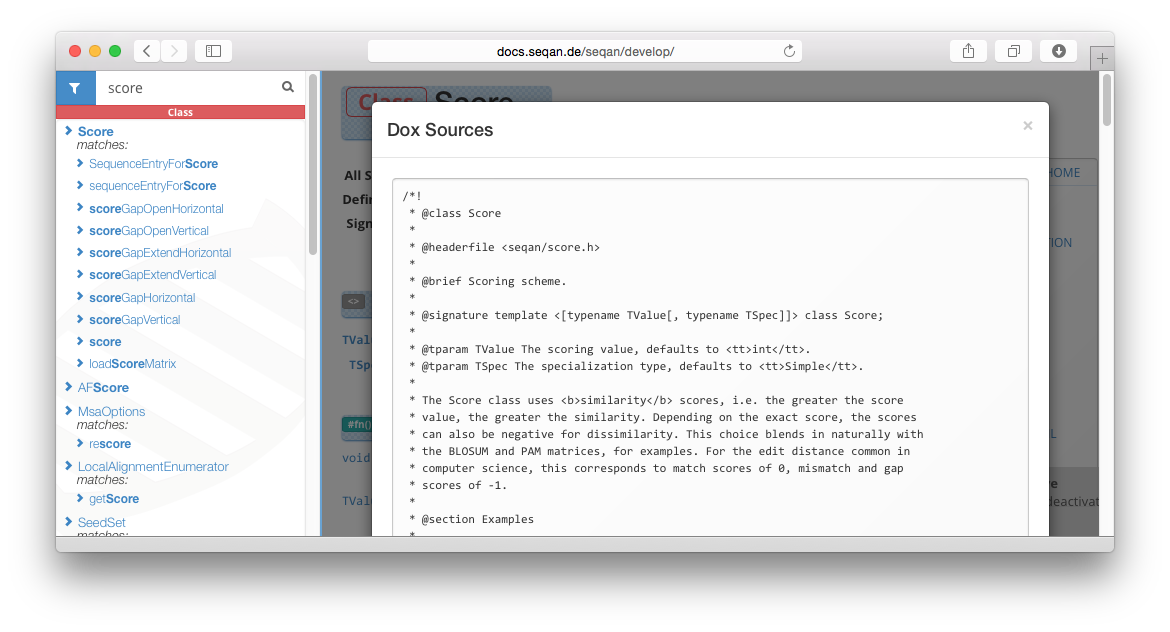
\includegraphics[width=0.9\linewidth]{Figures/dox/devmode-dox.png}
    \caption{Entwicklermodus --- Dox-Quelle für den aktuellen Dokumentationseintrag}
    \label{fig:dox-devmode-dox}
\end{figure}

\begin{figure}[ht!]
  \centering
    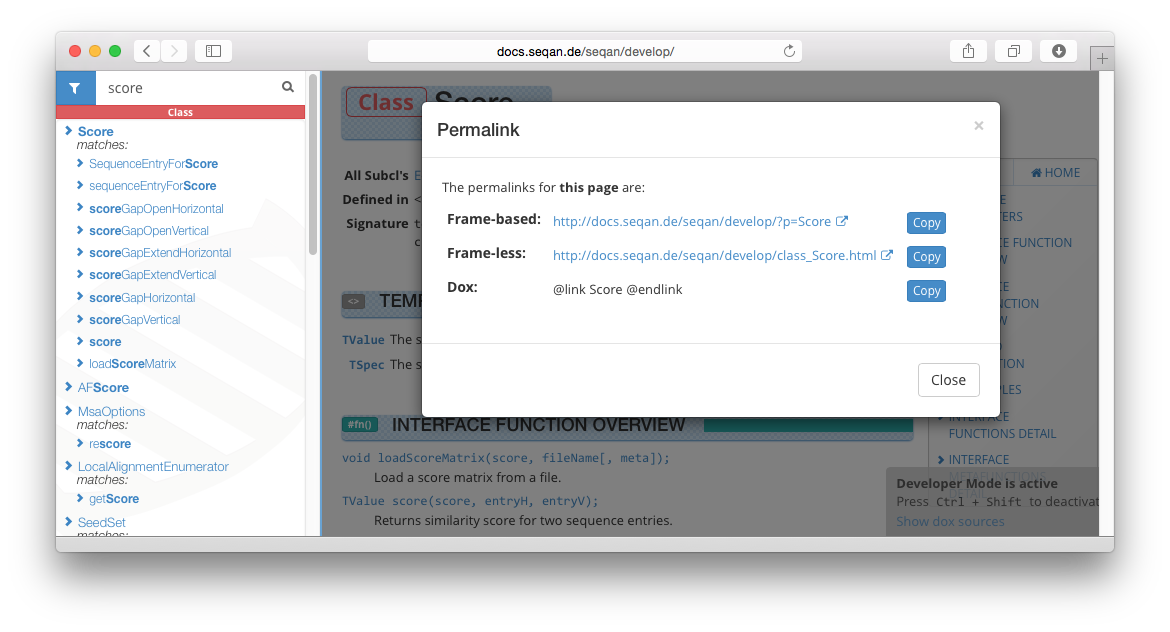
\includegraphics[width=0.9\linewidth]{Figures/dox/devmode-permalink.png}
    \caption[Entwicklermodus --- Anzeige aller Links für das aktuell selektierte Element]{Entwicklermodus: Anzeige aller Links für das aktuell selektierte Element. Im Hintergrund des modalen Dialogs kann man drei bläulich hinterlegte Elemente erkennen, die verlinkbar sind.}
    \label{fig:dox-devmode-permalink}
\end{figure}

%API-Entwickler müssen gute Dokumentation schreiben \citep{Kramer:1999ih}



\paragraph{Gesamtüberblick}

Die Notwendigkeit eines Gesamtüberblicks konnte ich empirisch zeigen und lässt sich auch direkt und indirekt aus der Literatur entnehmen. So verhindert ein fehlender Gesamtüberblick Top-Down-Lernen \citep[vgl.][]{Brooks:1983fj} und das Erkennen von Zusammengehörigkeit verteilter Informationen \citep[vgl.][]{BenShneiderman:gn} --- insbesondere für Anfänger \citep{Stylos:2008jt,Piccioni:2013uq}.

Werden an keiner Stelle Entwurfsentscheidungen gebündelt dargestellt, werden Anwender beim Anpassungen von Beispiel-Code eingeschränkt \citep{Bruch:2006bv}. Dies führt dazu, dass Anwender häufiger Fehler bei der Anpassung machen, und mit geringerer Wahrscheinlichkeit die korrekte Intention des Codes wiedergeben \citep{Fairbanks:2006jw}.

Außerdem muss die Startseite der Dokumentation über eine Aufgaben-bezogene, logische Gruppierung der Library-Elemente verfügen, da es klassenübergreifende Aufgaben gibt, deren Lösung sich für API-Anfänger sonst nicht ohne Weiteres erschließen würde. \citep{DaqingHou:2005ba,clarke:2006}

Die überarbeitete Startseite der SeqAn-Dokumentation verfügt nun über folgende Elemente:
\begin{itemize}\itemsep1pt\parskip0pt\parsep0pt
  \item Knappe Beschreibung von SeqAn
  \item \textit{Getting Started}
  \begin{itemize}
    \item Verweis auf die Installationsanleitungen
    \item Verweise auf die Tutorials und ähnliche Inhalte (Profiling, CMake, etc.)
    \item Verweis auf die Sprachentitätstypen-Übersichtseite
  \end{itemize}
  \item Typische SeqAn-Aufgaben mit Verweisungen auf die dazugehörigen Tutorials, Klassen und Funktionen. Die vier typischen Aufgaben lauten:
  \begin{itemize}
    \item Read-Mapping
    \item Ein- u. Ausgabe
    \item Sequence-Alignment
    \item Graphen
  \end{itemize}
\end{itemize}

Des Weiteren wurde das kaum auffindbare und veraltete Background-and-Motivation-Tutorial\footnote{\url{http://seqan.readthedocs.org/en/master/Tutorial/BackgroundAndMotivation.html}} umfassend überarbeitet. Es erklärt nun die Motivation der SeqAn zu Grunde liegenden Entwurfsentscheidungen und veranschaulicht den SeqAn-Performance-Gewinn an Hand eines ohne SeqAn geschriebenen Beispiels.

%High-level Design-Dokumentation notwendig \citep{Robillard:2009cs}
%Globale Designentscheidungen müssen auf Startseite der Doku erklärt werden \citep{Robillard:2009cs}




\paragraph{Sprachentitätstypen}

Das Konzept der \code{apiua://code/-9223372036854775413} (engl. \textit{language entity types}) ist in SeqAn von besonders großer Relevanz, da SeqAn durch den Gebrauch von Concepts Sprachentitätstypen verwendet, die dem Gros der SeqAn-Anwender unbekannt sind (siehe \sref{sec:gt-let}). Dabei ist es von elementarer Wichtigkeit, bedeutende Konzepte in einer Dokumentation zu erklären \citep{Jeong:kf,Ko:2011vw,Monperrus:2011bf}.

Mein Ziel war es, Anwender unaufdringlich auf die Existenz neuer Sprachentitätstypen hinzuweisen und es ihnen zu erlauben, sich auf leichtgewichtige Art darüber zu informieren. Dieser Ansatz wird als \textit{knowledge pushing} bezeichnet und wurde bereits in ähnlicher Weise von \cite{Watson:2009da,sunshine2014searching} erfolgreich angewendet.

Die Umsetzung erfolgte wie folgt:
\begin{itemize}
  \item Alle in der Dokumentation genannten Sprachentitäten, wie \texttt{length} oder \texttt{String}, werden durch ein kleines Label annotiert.
  \item Jedes Label kennzeichnet einen Sprachentitätstyp.
  \item Die Labels werden durch zwei Merkmale unterschieden:
  \begin{enumerate}
    \item Farbe, welche die Zusammengehörigkeit verschiedener Sprachentitätstypen symbolisiert.
    \item Ideogramm, also ein textuelles Piktogramm, das den Sprachentitätstyp phänotypisch ausdrückt.
  \end{enumerate}
  \item Die existierenden Sprachentitätstypen lauten:
  \begin{itemize}
    \item[] \raisebox{-0.4ex}{
\includegraphics[height=1em]{Figures/lets/typedef.png}} Typdefinition mittels \texttt{typedef}
    \hspace{1em} \raisebox{-0.4ex}{
\includegraphics[height=1em]{Figures/lets/variable.png}} Variable\footnote{Beim Schreiben dieser Dissertation wurde mir klar, dass \textit{var} ein geeigneteres Ideogramm darstellt. Ein entsprechender Issue-Tracker-Eintrag existiert: \url{https://github.com/seqan/seqan/issues/1034}}
    
    \item[] \raisebox{-0.4ex}{
\includegraphics[height=1em]{Figures/lets/concept.png}} Concept
    \hspace{1em} \raisebox{-0.4ex}{
\includegraphics[height=1em]{Figures/lets/class.png}} Klasse
    \hspace{1em} \raisebox{-0.4ex}{
\includegraphics[height=1em]{Figures/lets/spec.png}} Spezialisierung
    \hspace{1em} \raisebox{-0.4ex}{
\includegraphics[height=1em]{Figures/lets/enum.png}} Enum
    
    \item[] \raisebox{-0.4ex}{
\includegraphics[height=1em]{Figures/lets/globalmetafunction.png}} Globale Metafunktion
    \hspace{1em} \raisebox{-0.4ex}{
\includegraphics[height=1em]{Figures/lets/interfacemetafunction.png}} Interface-Metafunktion
    \hspace{1em} \raisebox{-0.4ex}{
\includegraphics[height=1em]{Figures/lets/tag.png}} Tag
    
    \item[] \raisebox{-0.4ex}{
\includegraphics[height=1em]{Figures/lets/globalfunction.png}} Globale Funktion
    \hspace{1em} \raisebox{-0.4ex}{
\includegraphics[height=1em]{Figures/lets/interfacefunction.png}} Interface-Funktion
    \hspace{1em} \raisebox{-0.4ex}{
\includegraphics[height=1em]{Figures/lets/memberfunction.png}} Member-Funktion

    \item[] \raisebox{-0.4ex}{
\includegraphics[height=1em]{Figures/lets/adaption.png}} Adaption
    \hspace{1em} \raisebox{-0.4ex}{
\includegraphics[height=1em]{Figures/lets/makro.png}} Makro
  \end{itemize}
  \item Bewegt der Anwender die Maus über ein Label, wird eine minimale Beschreibung des dazugehörigen Sprachentitättyps eingeblendet (siehe \fref{fig:dox-let-hover}).
  \item Klickt der Anwender bei eingeblendeter minimaler Beschreibung auf das Label, wird die ausführlichere Beschreibung des Sprachentitättyps geöffnet (siehe \fref{fig:dox-let-detail}).
  \item Sowohl Suchergebnisse als auch Funktionsauflistungen innerhalb von Dokumentationseinträgen sind nach den Sprachentitätstypen gruppiert (siehe \fref{fig:dox-large-string-opened-3.0.0}).
  \item Die Suchfunktion der Dokumentation erlaubt die Filterung der Ergebnisse nach Sprachentitätstypen. Tatsächlich ging es mir aber nicht um die Funktion selbst, sondern darum, dass neugierige Anwender so auf eine vollständige Auflistung der in SeqAn präsenten Sprachentitätstypen stoßen, ohne sich mit diesen gleich aktiv auseinandersetzen zu müssen.
\end{itemize}

\begin{figure}[ht!]
  \centering
    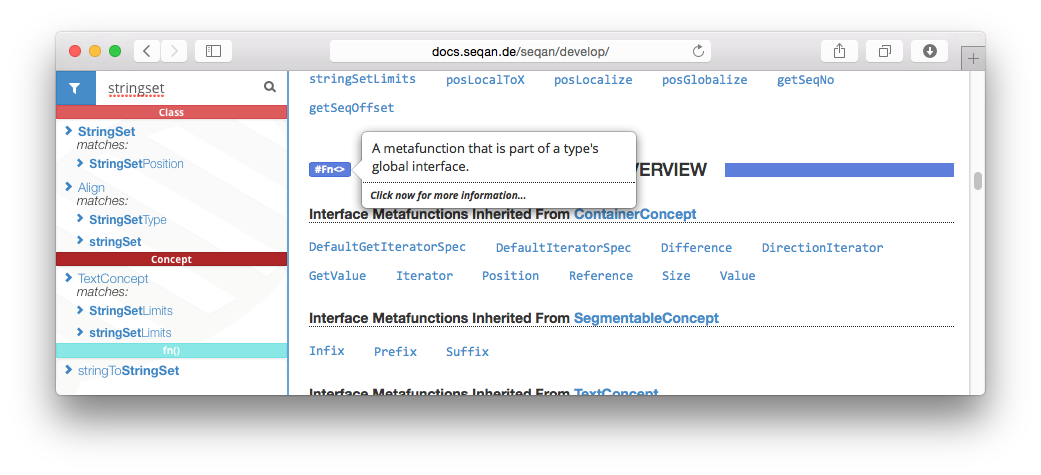
\includegraphics[width=0.9\linewidth]{Figures/dox/let-hover.png}
    \caption{Kurzbeschreibung des Sprachentitättyps \textit{Interface-Metafunktion}}
    \label{fig:dox-let-hover}
\end{figure}

\begin{figure}[ht!]
  \centering
    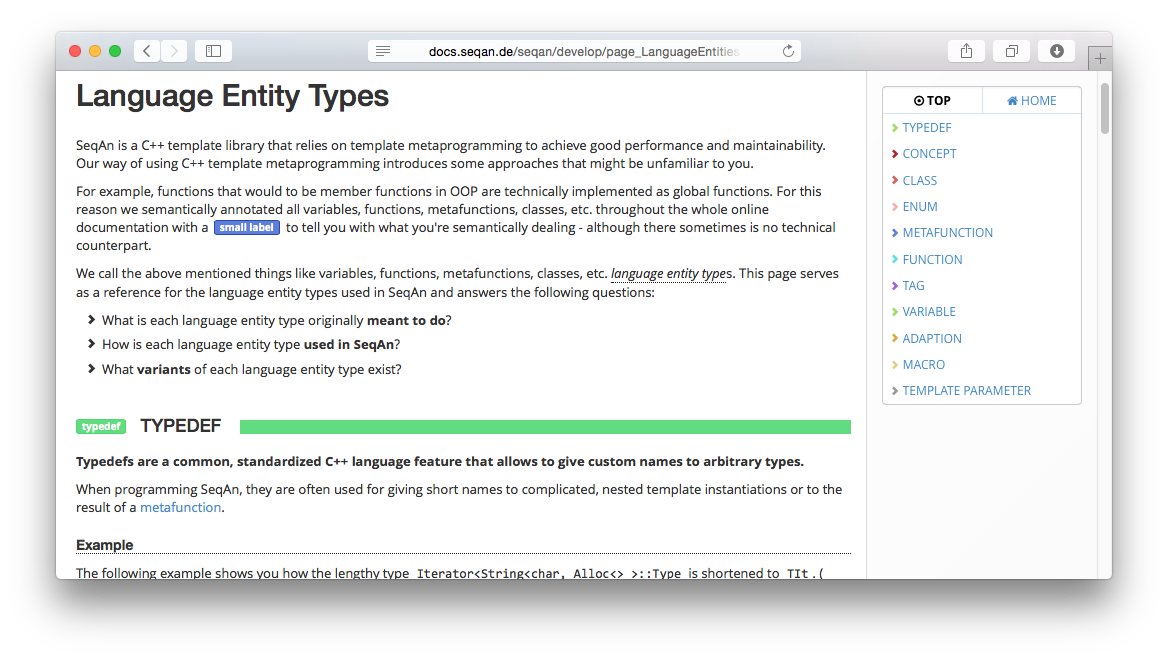
\includegraphics[width=0.9\linewidth]{Figures/dox/let-detail.png}
    \caption{Ausführliche Beschreibung der in SeqAn verwendeten Sprachentitätstypen}
    \label{fig:dox-let-detail}
\end{figure}



\paragraph{Seitenaufbau}

Der Aufbau von Dokumentationsseiten wurde von mir und einem SeqAn-Entwickler überarbeitet. Abstrakt sind Seiten wie folgt gegliedert:
\begin{enumerate}
\itemsep1pt\parskip0pt\parsep0pt
  \item Zusammenfassung zum Nachschlagen
  \item Detaillierte Beschreibung
\end{enumerate}

Im Grunde gibt es zwei Seitentypen:
\begin{description}
  \item[Containerseiten] kommen zur Dokumentation von Concepts, Klassen und Spezialisierungen zum Einsatz\footnote{Beispiel String-Klasse: \url{http://docs.seqan.de/seqan/develop/?p=String}}, da diese Sprachentitätstypen über Untereinträge verfügen. Hierbei umfasst die Zusammenfassung einen Bereich für Metainformationen und eine Auflistung aller verfügbaren Funktionen. Die Metainformationen zählen bei Klassen beispielsweise auf, welche Concepts direkt und indirekt implementiert werden, welche Spezialisierungen existieren, in welcher Datei die Klasse definiert ist und welche Signatur die Klasse besitzt. Die Auflistung der Funktionen ist gegliedert nach Member-Funktionen, Interface-Funktionen und Interface-Metafunktionen. Der Detailbereich erläutert im Falle einer Klasse den Gebrauch der Klasse samt Beispielen und erklärt detailliert sämtliche oben genannten Funktionen im Detail.
  \item[Elementseiten] sind atomar und kommen für alle anderen Sprachentitätstypen zum Einsatz\footnote{Beispiel globalAlignment-Funktion: \url{http://docs.seqan.de/seqan/develop/?p=globalAlignment}}, da diese über keine Untereinträge verfügen. Im Falle von (semantisch) globalen Funktionen umfasst die Zusammenfassung eine Auflistung aller Parameter und die Beschreibung der Rückgaben. Der Detailbereich erläutert dann wiederum ausführlich Sinn und Zweck der Funktion und beschreibt dies an Hand von Beispielen.
\end{description}

In SeqAn werden häufig Referenzen technisch als Eingaben übergeben, inhaltlich aber als Rückgaben behandelt. Ob ein Parameter als Ein- und/oder Ausgabe behandelt wird, wird durch die folgenden Icons ausgezeichnet: 
\includegraphics[height=.7em]{Figures/dox/in.png}, 
\includegraphics[height=.7em]{Figures/dox/out.png} und 
\includegraphics[height=.7em]{Figures/dox/inout.png}.


\paragraph{Beispiele}

Beispiele sind neben der Gesamtübersicht der wichtigste Bestandteil einer benutzerfreundlichen Dokumentation \citep{Robillard:2010bh}, was ich an Hand der verschiedenen, durch die Abwesenheit (guter) Beispiele eingeschränkten Beispiel-bezogenen Strategien empirisch belegen konnte (siehe \sref{sec:dox}).

Im Zuge der inhaltlichen Überarbeitung der Dokumentation wurden für die wichtigsten Dokumentationseinträge existierende Beispiele verbessert und fehlende Beispiele ergänzt. Dabei wurden alle Beispiele um die Programmausgabe ergänzt, was besonders für API-Endanwender wichtig ist \citep{Gross:2010iz}.



\paragraph{Suchfunktion}

Die vollständig neu entwickelte Suchfunktion verfügt über die folgenden Funktionen:
\begin{itemize}
  \item Sprachentitäten können nun über Aliasse/Synonyme verfügen. Auf diese Weise wurden die im \textit{Vocabulary Problem} \citep{Furnas:1987hl} veranlagten Usability-Probleme gemildert. Der Suchbegriff \texttt{substring} beispielweise führt nun auch zu dem Treffer \textit{infix}. Wurde ein Eintrag mit Hilfe eines Synonyms gefunden, wird dem Anwender dies mitgeteilt. Auf diese Weise lernt der Anwender bedarfsgerecht die korrekte Bezeichnung in SeqAn. Anwender, die ohnehin den korrekten Begriff verwendet haben, erfahren nicht von den Synonymen. Auf diese Weise wird verhindert, dass unterschiedlich benannte, aber inhaltlich identische Sprachentitäten innerhalb von SeqAn gepflegt werden müssen.
  \item Die Suchergebnisse sind nun gewichtet, so dass beispielsweise der Suchbegriff \texttt{string} auch tatsächlich die \texttt{String}-Klasse als ersten Suchtreffer hervorbringt.
  \item Die Suchergebnisse sind nach Sprachentitätstypen gruppiert und auf maximal fünf Einträge je Typ begrenzt. Auslassungspunkte am Ende einer Treffergruppe deuten darauf hin. Ein Klick darauf zeigt alle Suchtreffer der Gruppe.
  \item Suchergebnisse können auch Dokumentationsteileinträge sein. So ist der erste Suchtreffer für \texttt{infix}, die \texttt{Infix}-Interface-Metafunktion innerhalb des Concepts \texttt{SegmentableConcept}. Der Anwender kann selbst wählen, ob der den Dokumentationseintrag oder -untereintrag öffnen möchte.
  \item Die Suche kann ohne Maus und ausschließlich mit der Tastatur bedient werden. Dazu erhält das Suchfeld automatisch den Fokus, die Sucheingabe kann mit \texttt{Esc} gelöscht und innerhalb der Suchergebnisse mit den Pfeiltasten navigiert werden.
\end{itemize}

  



\paragraph{Darstellung}

Die Online-Dokumentation ist \textit{responsive}\footnote{\url{https://developers.google.com/web/fundamentals/layouts/rwd-fundamentals/}}, passt sich also einer großen Bandbreite von Fenstergrößen an. Dies ist nicht nur schick, sondern auch hilfreich. Bei SeqAn-Anfängern konnte ich einen häufigen Wechsel zwischen Entwicklungsumgebung und Online-Dokumentation beobachten. Da die neue SeqAn-Dokumentation selbst bei einem 600 Pixel schmalen Fenster (bei 72 DPI) ohne Einschränkung nutzbar ist, können SeqAn-Anwender die Dokumentation auch neben der Entwicklungsumgebung platzieren. Auch ist eine Nutzung der Dokumentation auf mobilen Geräten möglich, wie es einige Anwender forderten.

Des Weiteren habe ich großen Wert auf eine hohe Ästhetik gelegt. Ich denke, dieses u.a. durch den Einsatz von subtilen Farbverläufen und dezenten Animationen erreicht zu haben. Spaß an der Bedienung ist ein wesentlicher Aspekt des Anwendererlebnisses und spielt damit auch für SeqAns kommerziellen Erfolg eine Rolle.

\fref{fig:dox-small-all} stellt die gleichen Inhalte wie \fref{fig:dox-large-all} auf Seite \pageref{fig:dox-large-all} dar --- nur mit dem Unterschied eines schmaleren Browser-Fensters.

\newgeometry{inner=2cm,outer=1cm,top=1.5cm,bottom=1.5cm}
\thispagestyle{empty}
%\begin{landscape}
\begin{figure}
        \centering
        \begin{subfigure}[b]{0.48\linewidth}
                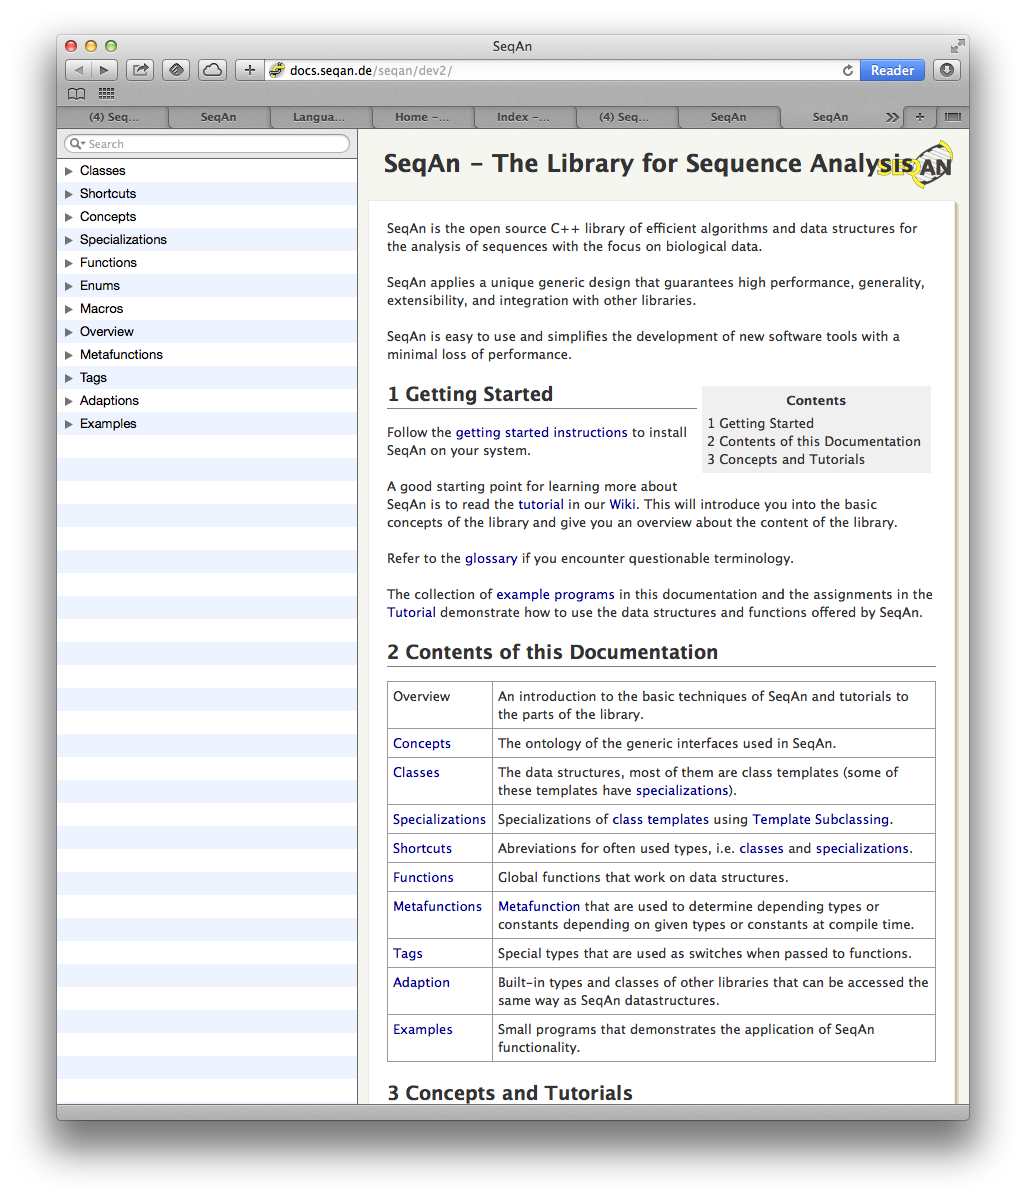
\includegraphics[width=\linewidth]{Figures/dox/dox-2_0_0-small-home.png}
                \caption{Startseite in Version 2.0.0}
                \label{fig:dox-small-home-2.0.0}
        \end{subfigure}
        \hfill
        \begin{subfigure}[b]{0.48\linewidth}
                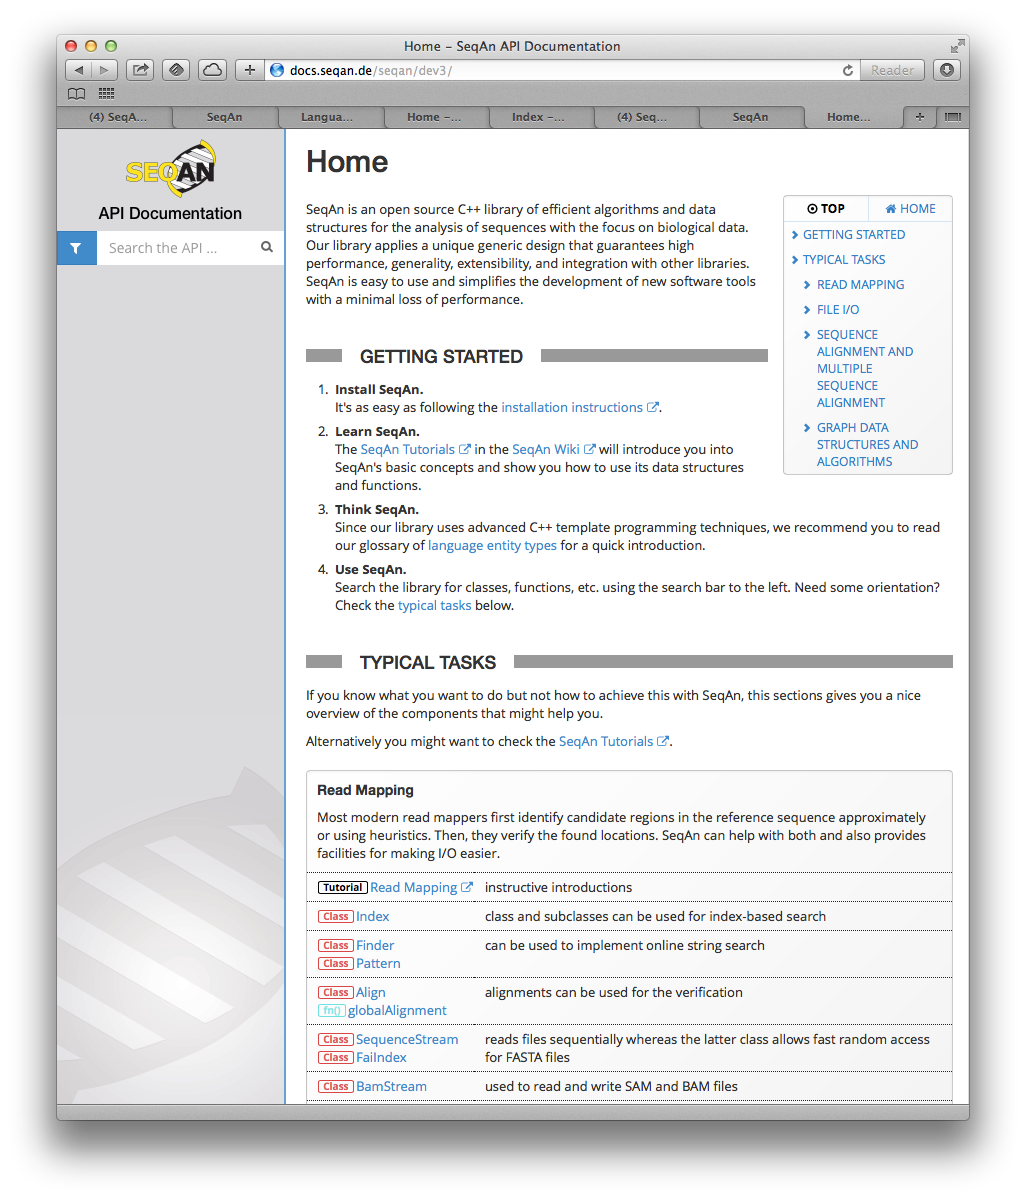
\includegraphics[width=\linewidth]{Figures/dox/dox-3_0_0-small-home.png}
                \caption{Startseite in Version 3.0.0}
                \label{fig:dox-small-home-3.0.0}
        \end{subfigure}%
        \vskip\baselineskip
        \begin{subfigure}[b]{0.48\linewidth}
                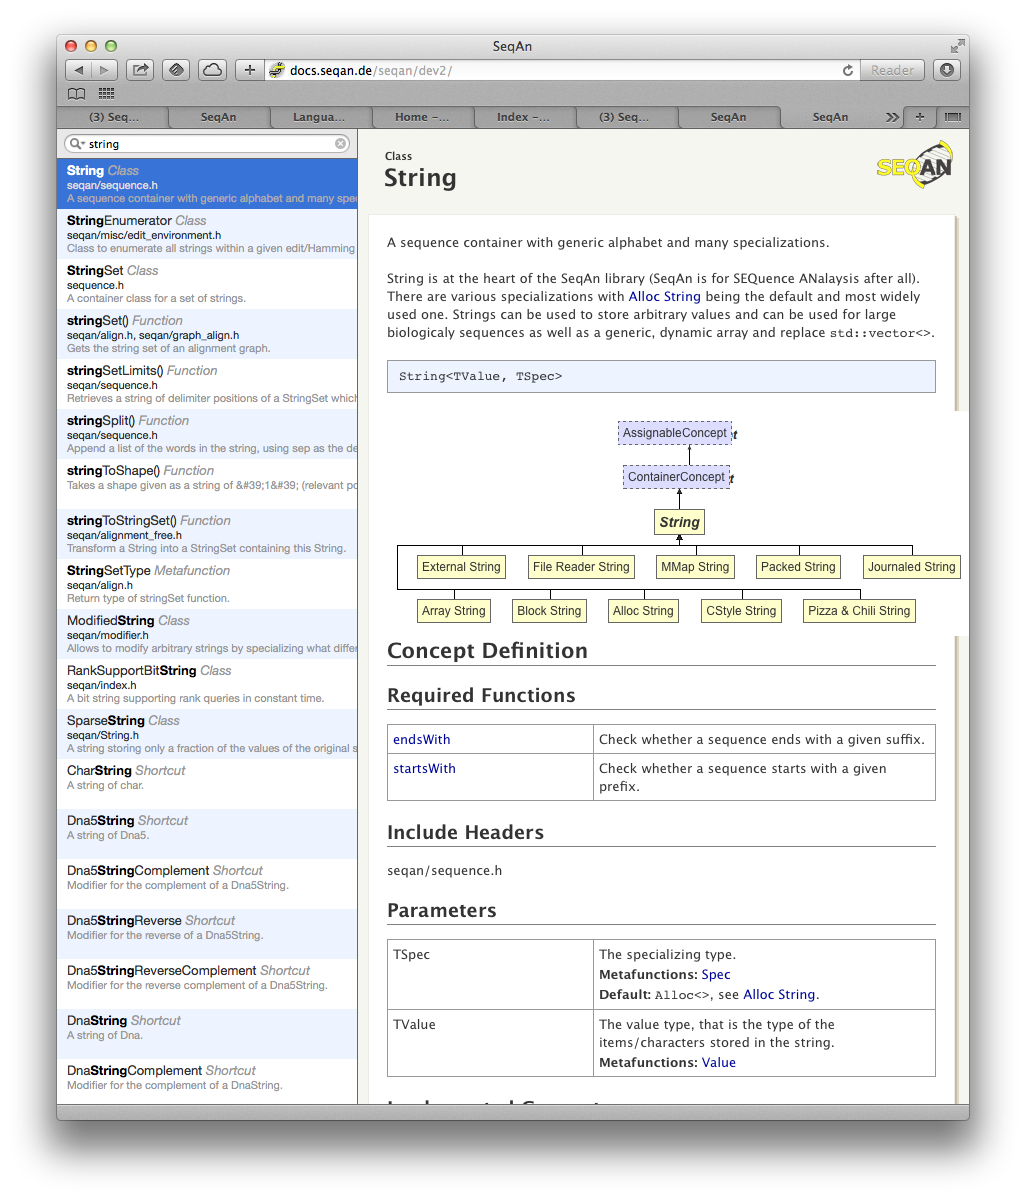
\includegraphics[width=\linewidth]{Figures/dox/dox-2_0_0-small-string-opened.png}
                \caption{Geöffnete \texttt{String}-Klasse in Version 2.0.0}
                \label{fig:dox-small-string-opened-2.0.0}
        \end{subfigure}
        \hfill
        \begin{subfigure}[b]{0.48\linewidth}
                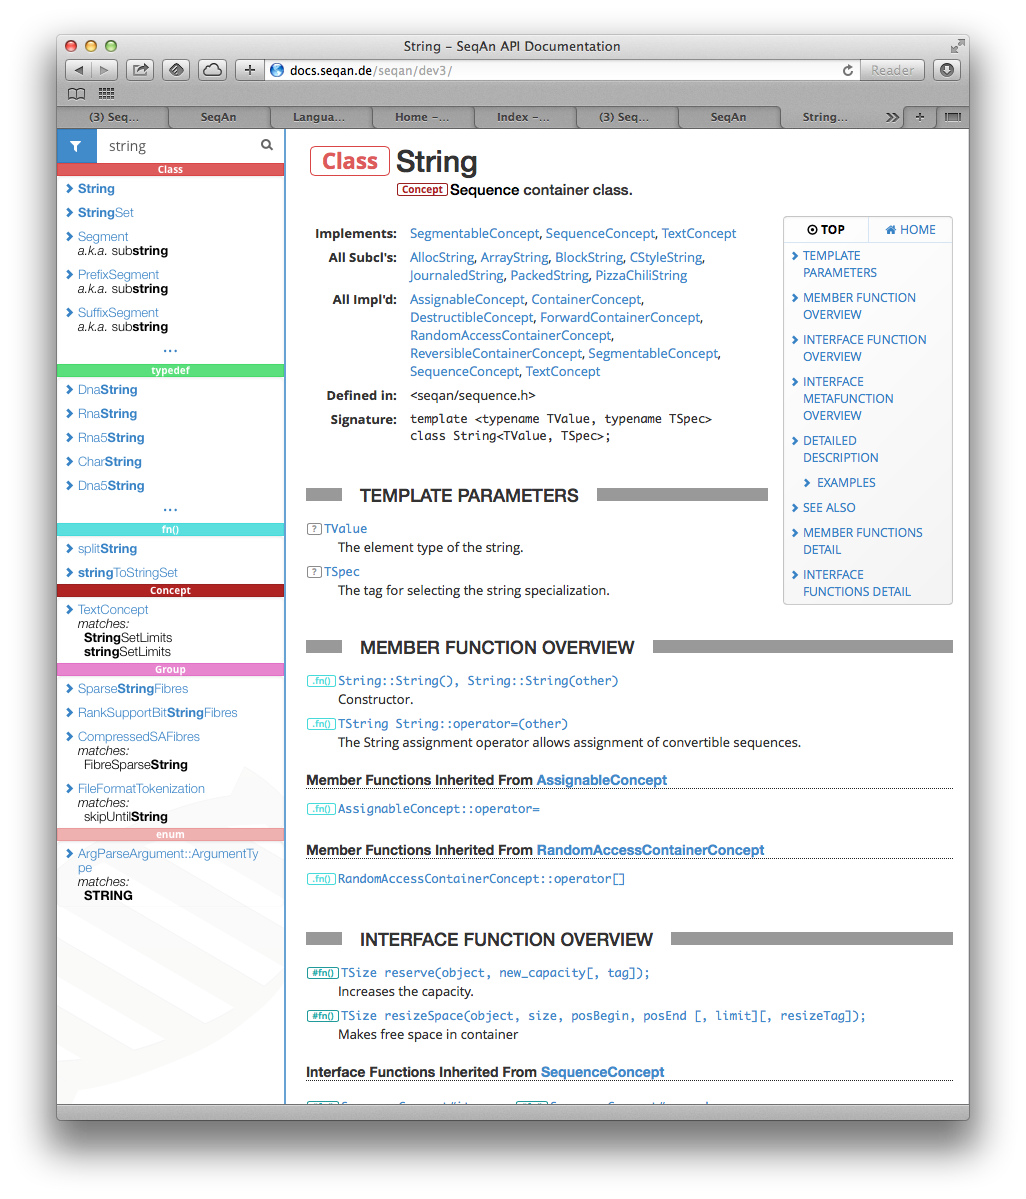
\includegraphics[width=\linewidth]{Figures/dox/dox-3_0_0-small-string-opened.png}
                \caption{Geöffnete \texttt{String}-Klasse in Version 3.0.0}
                \label{fig:dox-small-string-opened-3.0.0}
        \end{subfigure}
        \caption[Alte und neue Dokumentation im Vergleich --- in smaler Breite]{Die Abbildungen zeigen die alte und neue Dokumentation in schmaler Breite.}
        \label{fig:dox-small-all}
\end{figure}
%\end{landscape}
\restoregeometry




\paragraph{Integration}

Die neue Dokumentation ist besser in anderen Lernressourcen, wie den Tutorials, integriert. Dies wurde nicht zuletzt durch den weiter oben beschrieben Entwicklermodus gefördert, der SeqAn-Entwicklern alle möglichen Links für einen Dokumentations-(teil-)eintrag bereitstellt.  

Außerdem habe ich bei der Neuentwicklung auf die Indexierbarkeit durch Suchmaschinen geachtet. Dazu habe ich das Programm, welches die Dokumentation generiert, so angepasst, dass Inhalte sowohl statisch (für Suchmaschinen), als auch dynamisch (für Anwender) vorliegen.

Des Weiteren erfordert die Dokumentation --- trotz seines Funktionszuwachses --- keine Server-Komponente. Die mit SeqAn heruntergeladene Dokumentation verfügt online wie offline über den gleichen Funktionsumfang.







\begin{comment}
\newlength{\doxlargewidth}
\setlength{\doxlargewidth}{\linewidth}

\newlength{\doxnarrowwidth}
\setlength{\doxnarrowwidth}{0.61\doxlargewidth}

Donec urna leo, vulputate vitae porta eu, vehicula blandit libero. Phasellus eget massa et leo condimentum mollis. Nullam molestie, justo at pellentesque vulputate, sapien velit ornare diam, nec gravida lacus augue non diam. Integer mattis lacus id libero ultrices sit amet mollis neque molestie. Integer ut leo eget mi volutpat congue. Vivamus sodales, turpis id venenatis placerat, tellus purus adipiscing magna, eu aliquam nibh dolor id nibh. Pellentesque habitant morbi tristique senectus et netus et malesuada fames ac turpis egestas. Sed cursus convallis quam nec vehicula. Sed vulputate neque eget odio fringilla ac sodales urna feugiat.

\begin{figure}
  \centering
    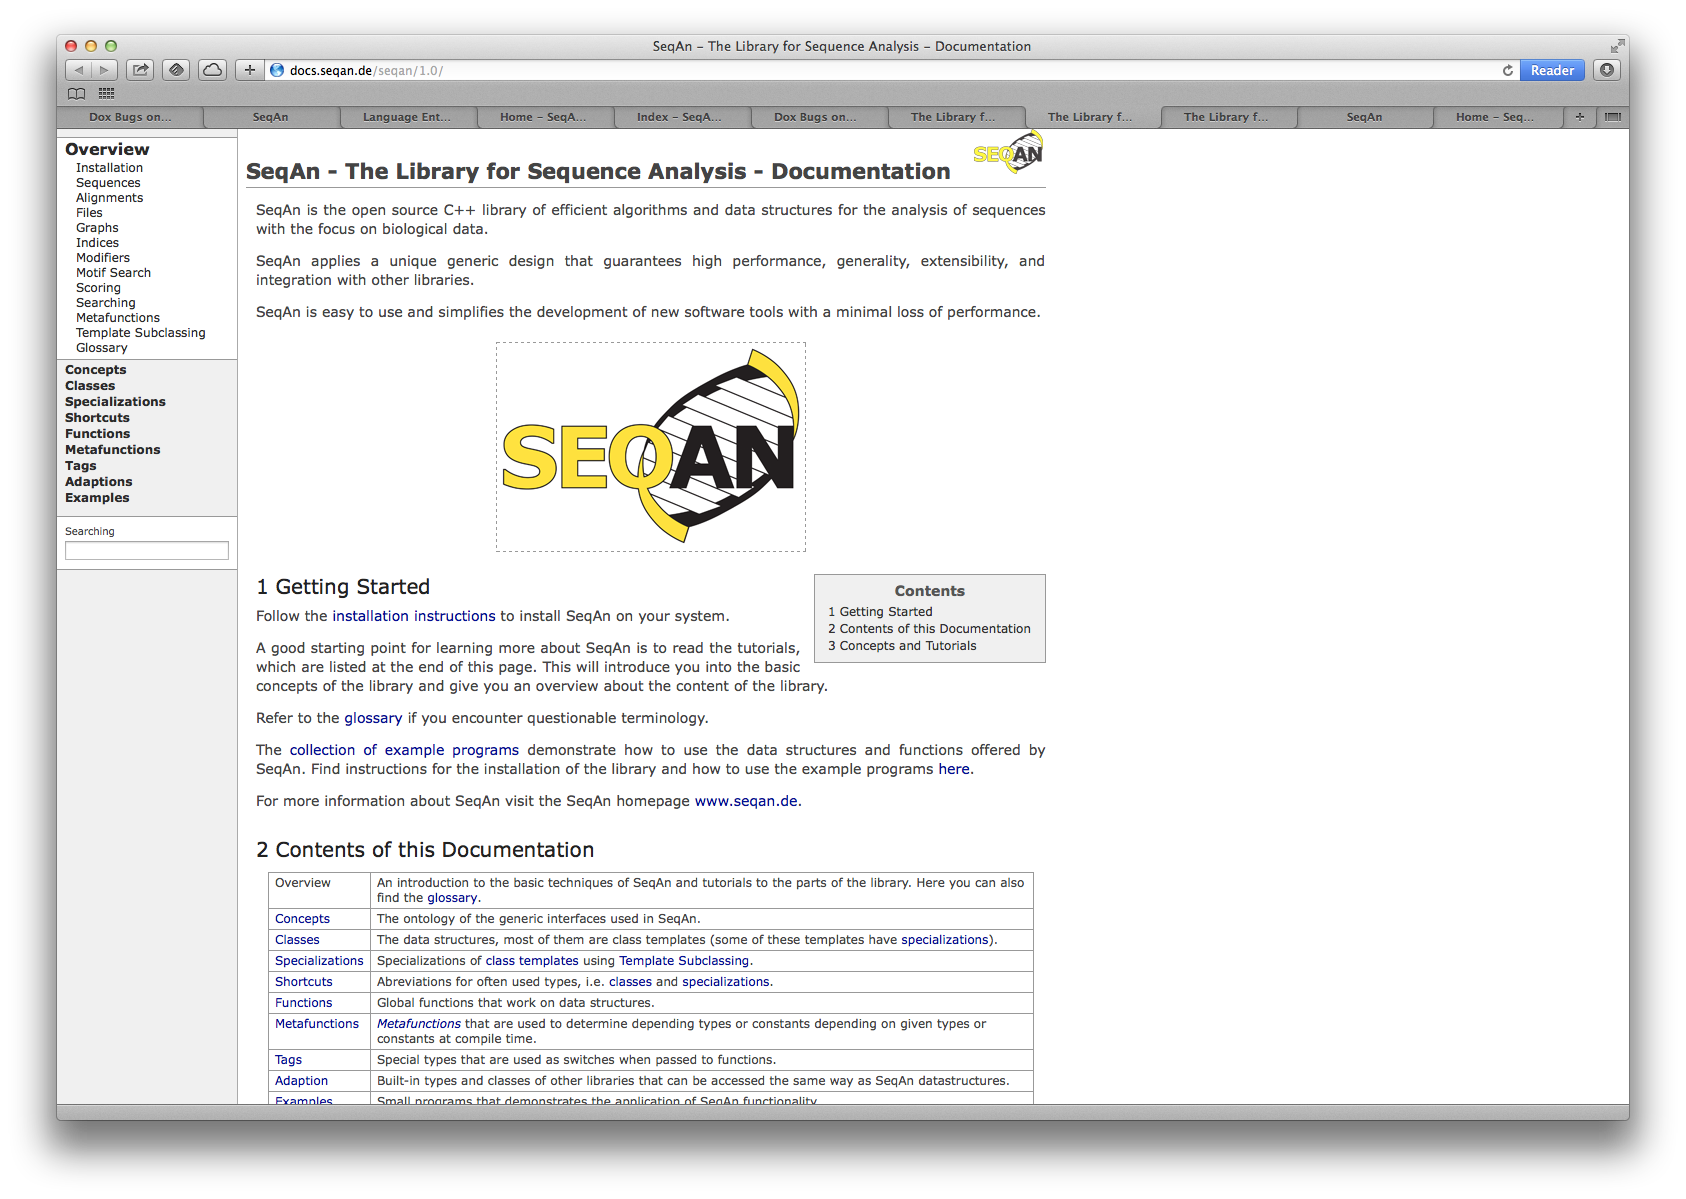
\includegraphics[width=\doxlargewidth]{Figures/dox/dox-1_0_0-large-home.png}
    \caption{Seqan-Online-Dokumentation in Version 1.0 - Breite Ansicht - Startseite}
    \label{fig:dox-1_0_0-large-home}
\end{figure}

\begin{figure}
  \centering
    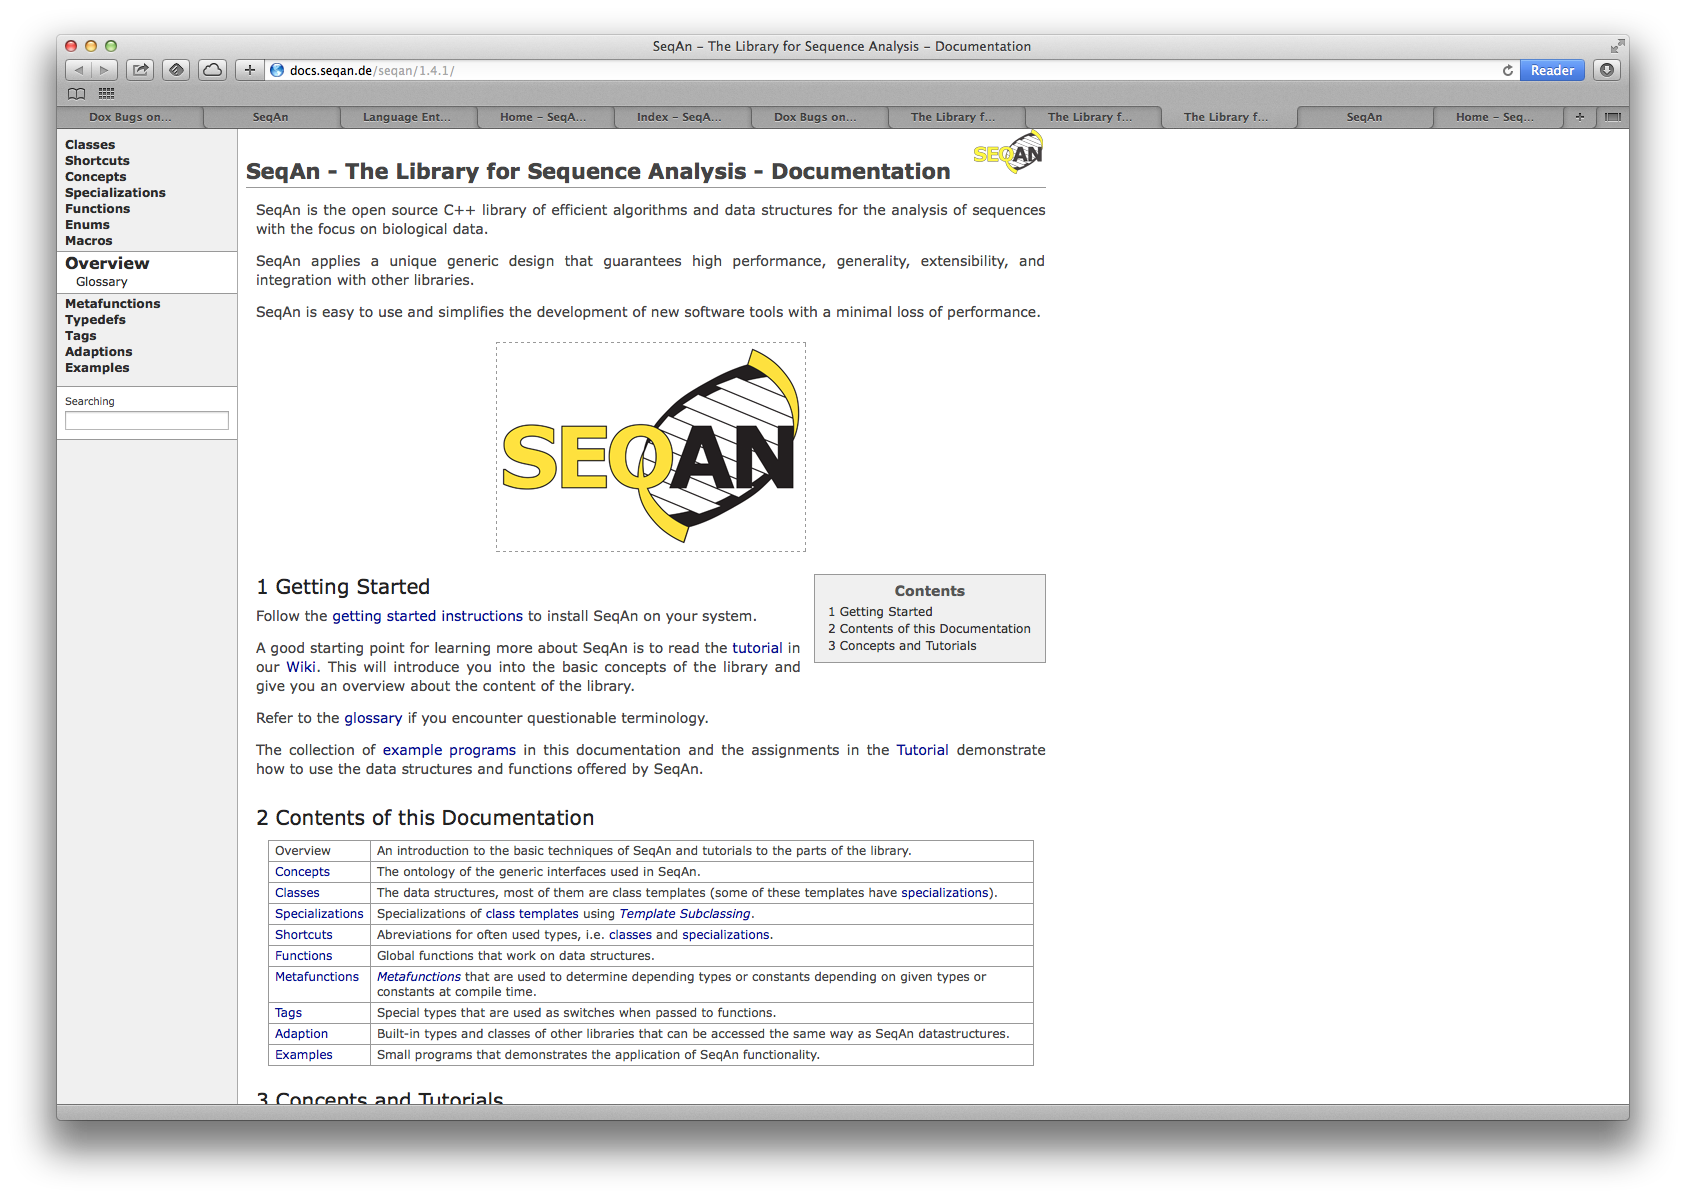
\includegraphics[width=\doxlargewidth]{Figures/dox/dox-1_4_1-large-home.png}
    \caption{Seqan-Online-Dokumentation in Version 1.4.1 - Breite Ansicht - Startseite}
    \label{fig:dox-1_4_1-large-home}
\end{figure}

Donec urna leo, vulputate vitae porta eu, vehicula blandit libero. Phasellus eget massa et leo condimentum mollis. Nullam molestie, justo at pellentesque vulputate, sapien velit ornare diam, nec gravida lacus augue non diam. Integer mattis lacus id libero ultrices sit amet mollis neque molestie. Integer ut leo eget mi volutpat congue. Vivamus sodales, turpis id venenatis placerat, tellus purus adipiscing magna, eu aliquam nibh dolor id nibh. Pellentesque habitant morbi tristique senectus et netus et malesuada fames ac turpis egestas. Sed cursus convallis quam nec vehicula. Sed vulputate neque eget odio fringilla ac sodales urna feugiat.

\begin{figure}
  \centering
    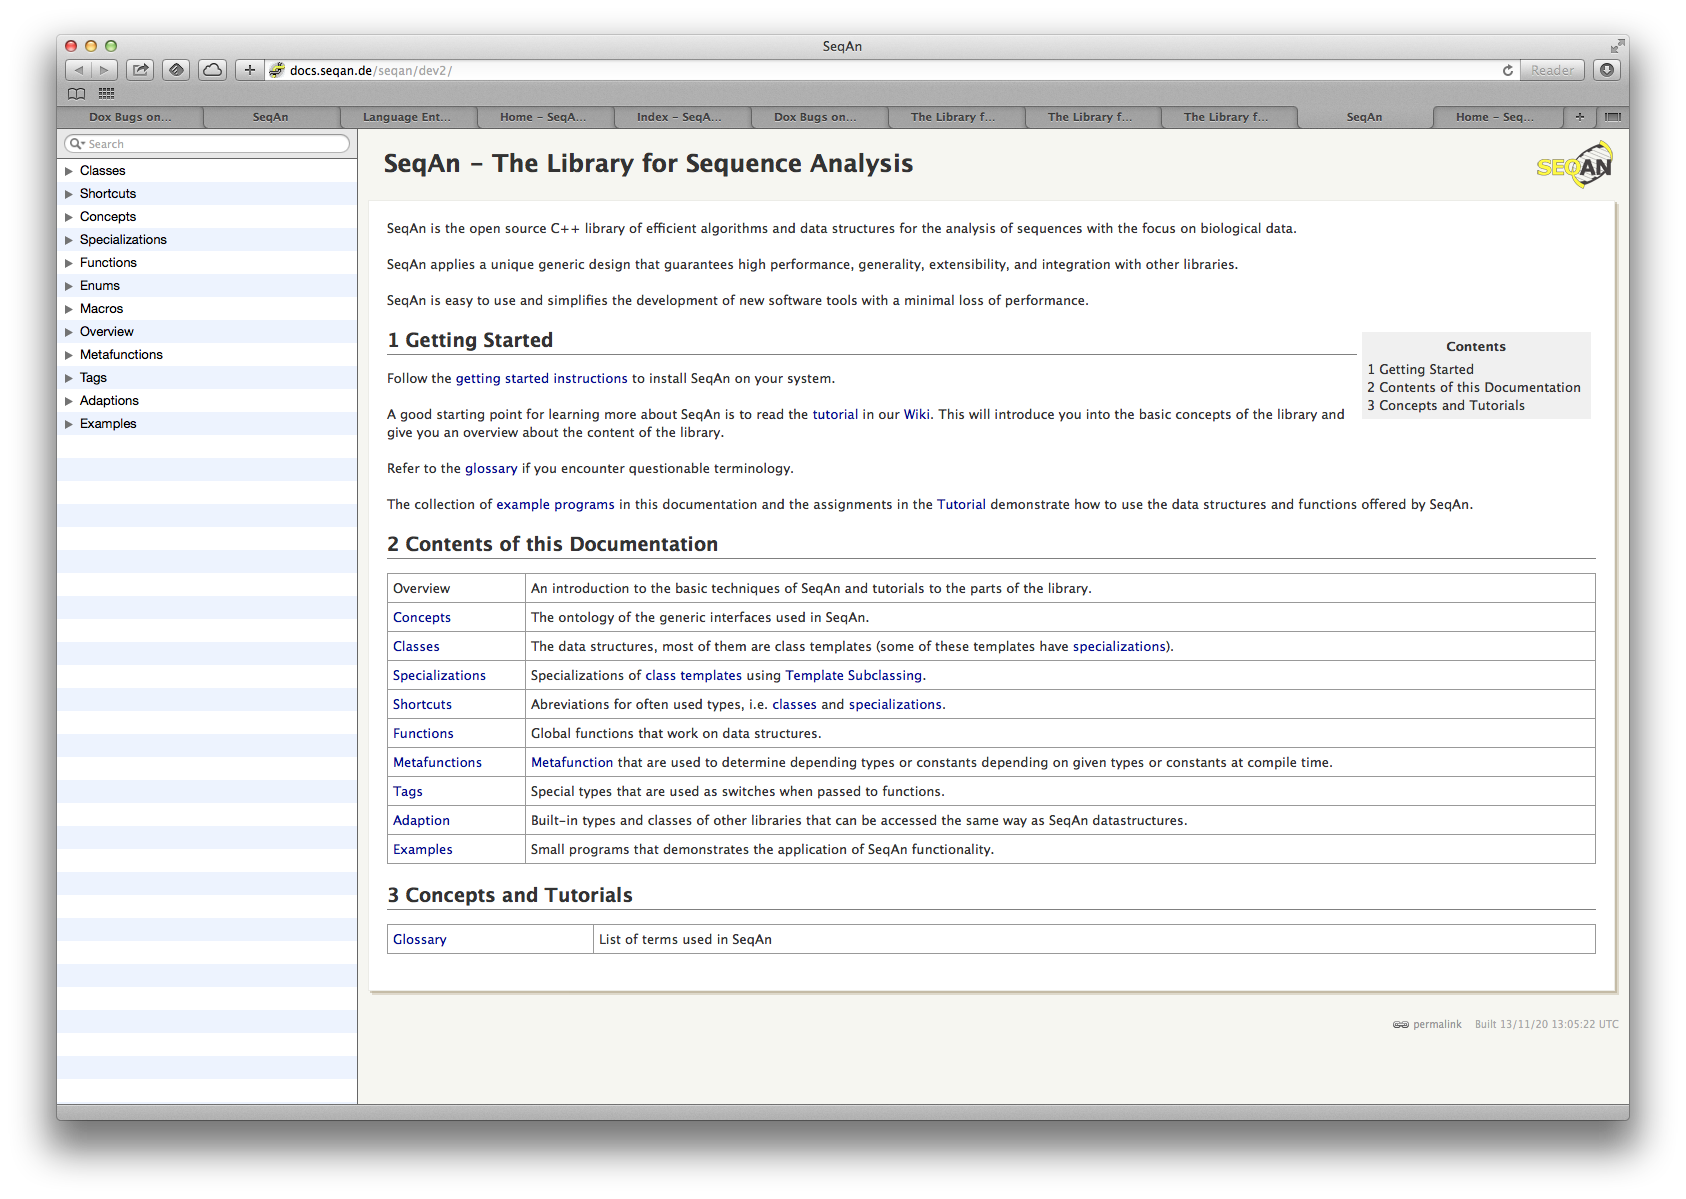
\includegraphics[width=\doxlargewidth]{Figures/dox/dox-2_0_0-large-home.png}
    \caption{Seqan-Online-Dokumentation in Version 2.0 - Breite Ansicht - Startseite}
    \label{fig:dox-2_0_0-large-home}
\end{figure}

\begin{figure}
  \centering
    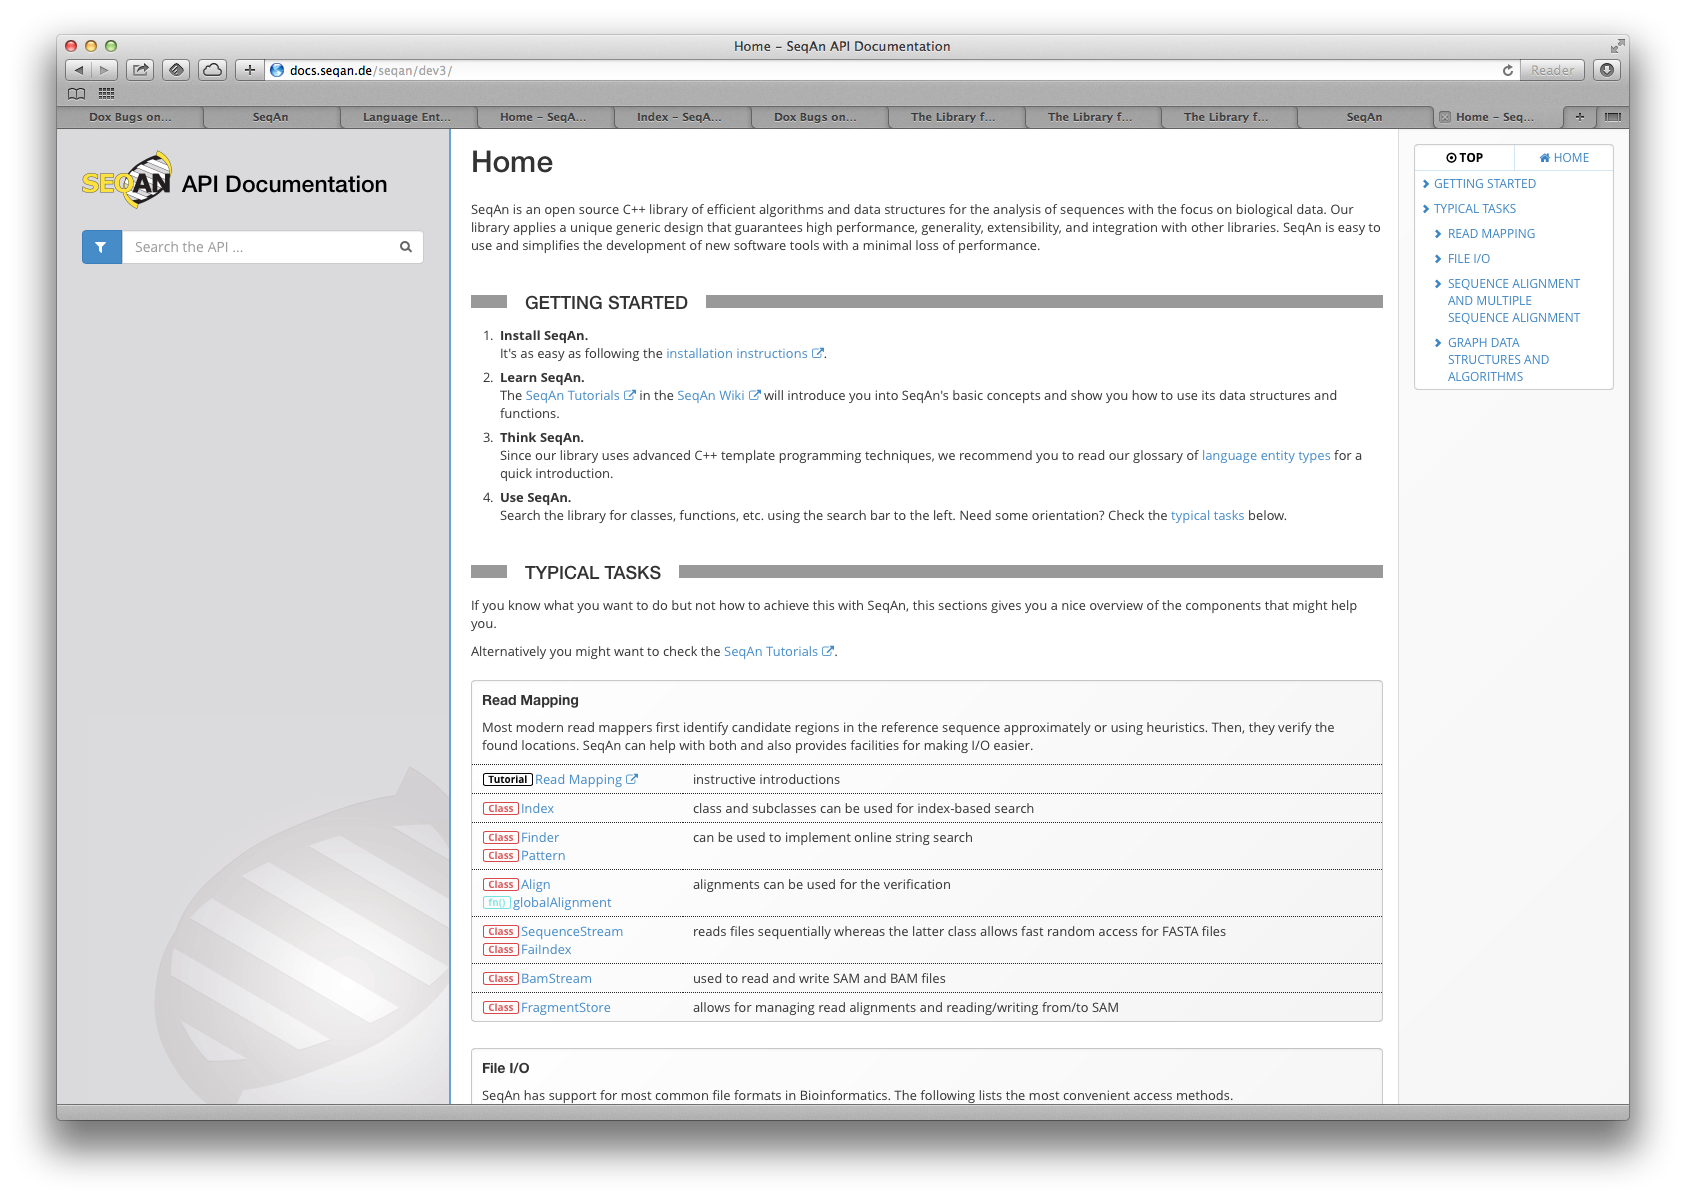
\includegraphics[width=\doxlargewidth]{Figures/dox/dox-3_0_0-large-home.png}
    \caption{Seqan-Online-Dokumentation in Version 3.0 - Breite Ansicht - Startseite}
    \label{fig:dox-3_0_0-large-home}
\end{figure}

Donec urna leo, vulputate vitae porta eu, vehicula blandit libero. Phasellus eget massa et leo condimentum mollis. Nullam molestie, justo at pellentesque vulputate, sapien velit ornare diam, nec gravida lacus augue non diam. Integer mattis lacus id libero ultrices sit amet mollis neque molestie. Integer ut leo eget mi volutpat congue. Vivamus sodales, turpis id venenatis placerat, tellus purus adipiscing magna, eu aliquam nibh dolor id nibh. Pellentesque habitant morbi tristique senectus et netus et malesuada fames ac turpis egestas. Sed cursus convallis quam nec vehicula. Sed vulputate neque eget odio fringilla ac sodales urna feugiat.

Donec urna leo, vulputate vitae porta eu, vehicula blandit libero. Phasellus eget massa et leo condimentum mollis. Nullam molestie, justo at pellentesque vulputate, sapien velit ornare diam, nec gravida lacus augue non diam. Integer mattis lacus id libero ultrices sit amet mollis neque molestie. Integer ut leo eget mi volutpat congue. Vivamus sodales, turpis id venenatis placerat, tellus purus adipiscing magna, eu aliquam nibh dolor id nibh. Pellentesque habitant morbi tristique senectus et netus et malesuada fames ac turpis egestas. Sed cursus convallis quam nec vehicula. Sed vulputate neque eget odio fringilla ac sodales urna feugiat.


\begin{figure}
  \centering
    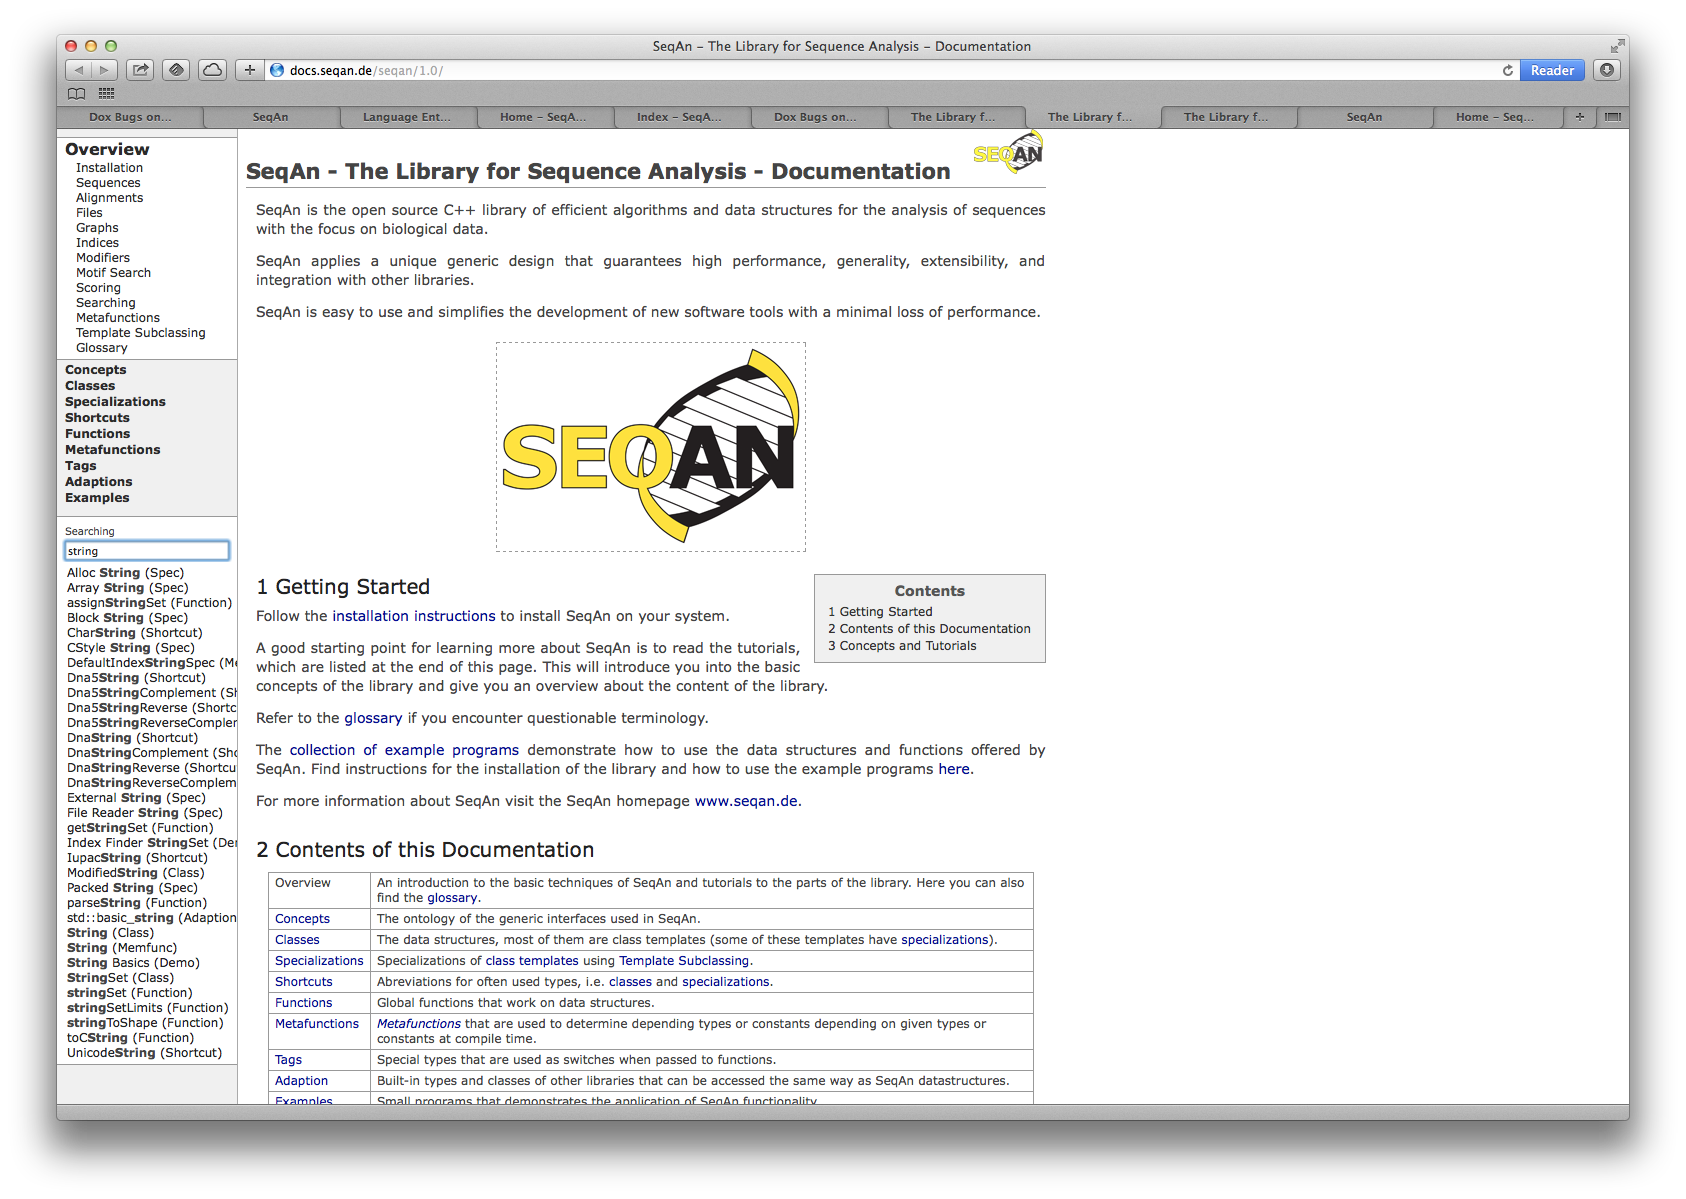
\includegraphics[width=\doxlargewidth]{Figures/dox/dox-1_0_0-large-string.png}
    \caption{Seqan-Online-Dokumentation in Version 1.0 - Breite Ansicht - Suche nach ``String''}
    \label{fig:dox-1_0_0-large-string}
\end{figure}

\begin{figure}
  \centering
    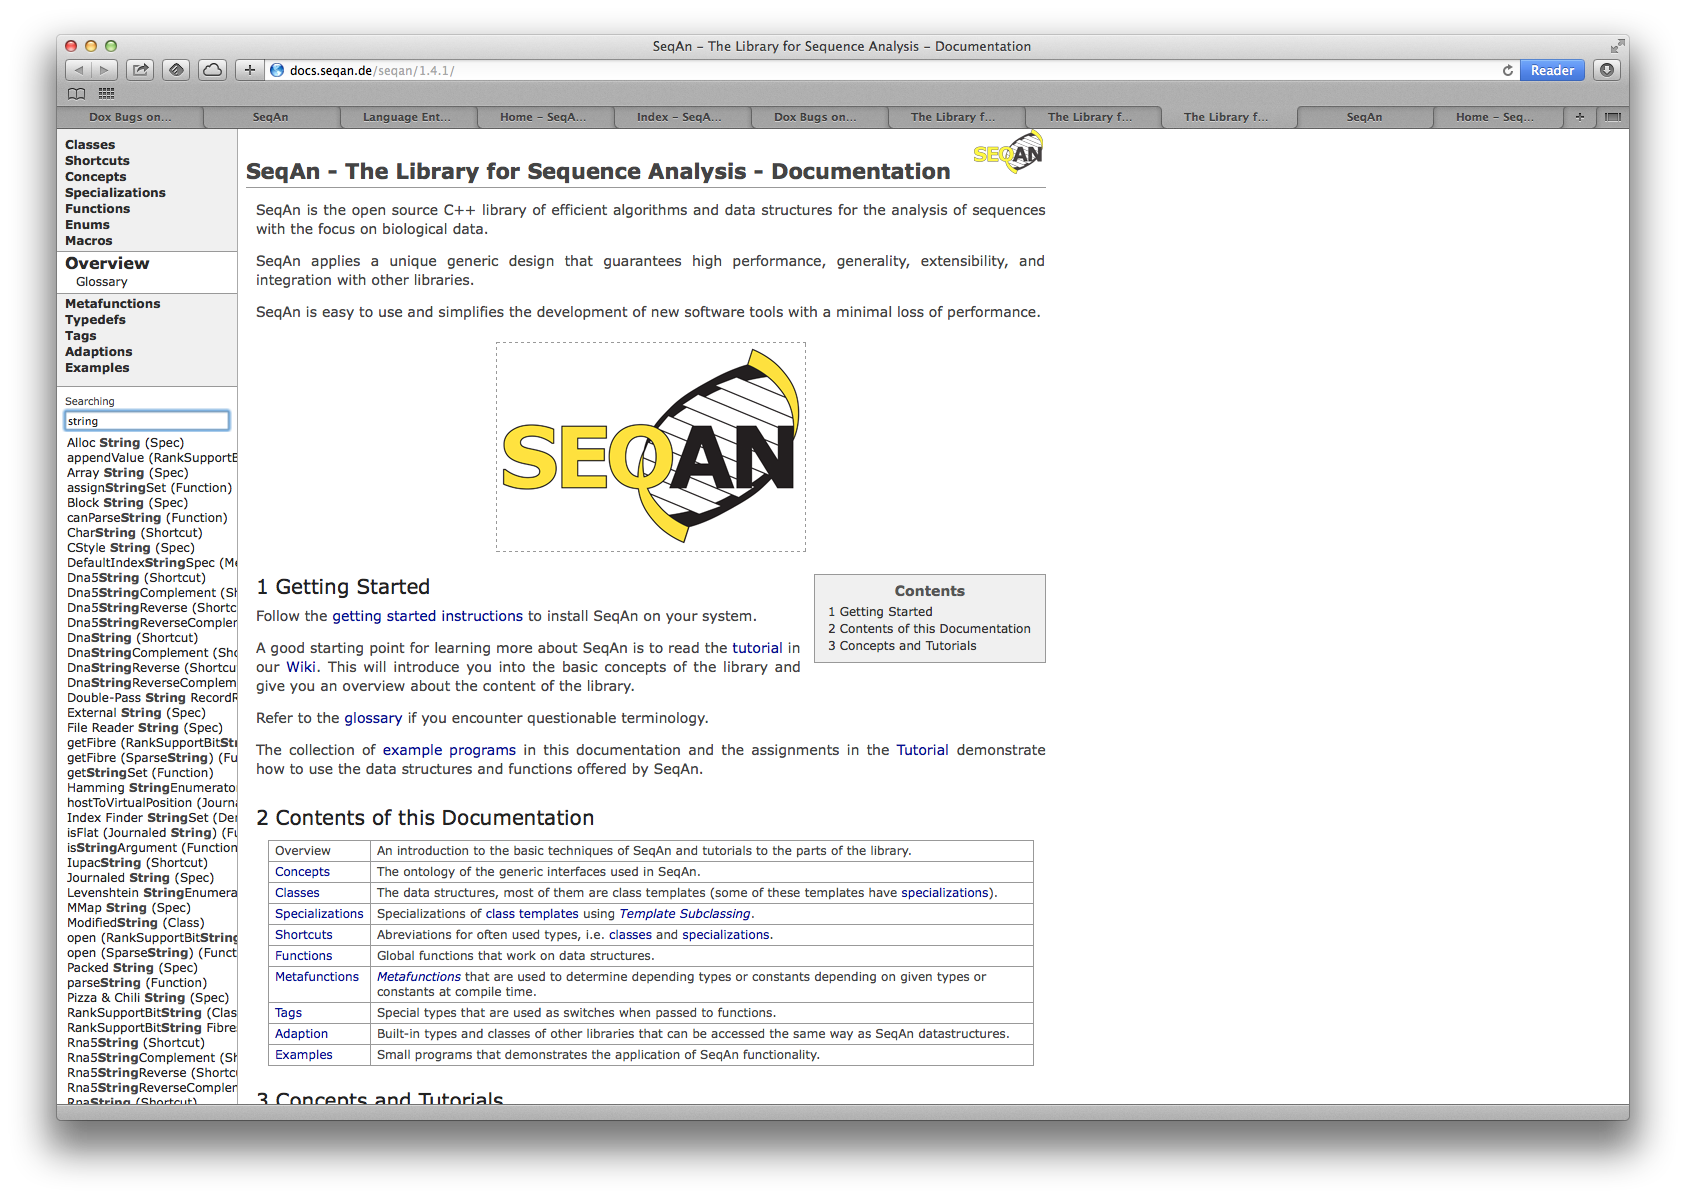
\includegraphics[width=\doxlargewidth]{Figures/dox/dox-1_4_1-large-string.png}
    \caption{Seqan-Online-Dokumentation in Version 1.4.1 - Breite Ansicht - Suche nach ``String''}
    \label{fig:dox-1_4_1-large-string}
\end{figure}

Donec urna leo, vulputate vitae porta eu, vehicula blandit libero. Phasellus eget massa et leo condimentum mollis. Nullam molestie, justo at pellentesque vulputate, sapien velit ornare diam, nec gravida lacus augue non diam. Integer mattis lacus id libero ultrices sit amet mollis neque molestie. Integer ut leo eget mi volutpat congue. Vivamus sodales, turpis id venenatis placerat, tellus purus adipiscing magna, eu aliquam nibh dolor id nibh. Pellentesque habitant morbi tristique senectus et netus et malesuada fames ac turpis egestas. Sed cursus convallis quam nec vehicula. Sed vulputate neque eget odio fringilla ac sodales urna feugiat.

\begin{figure}
  \centering
    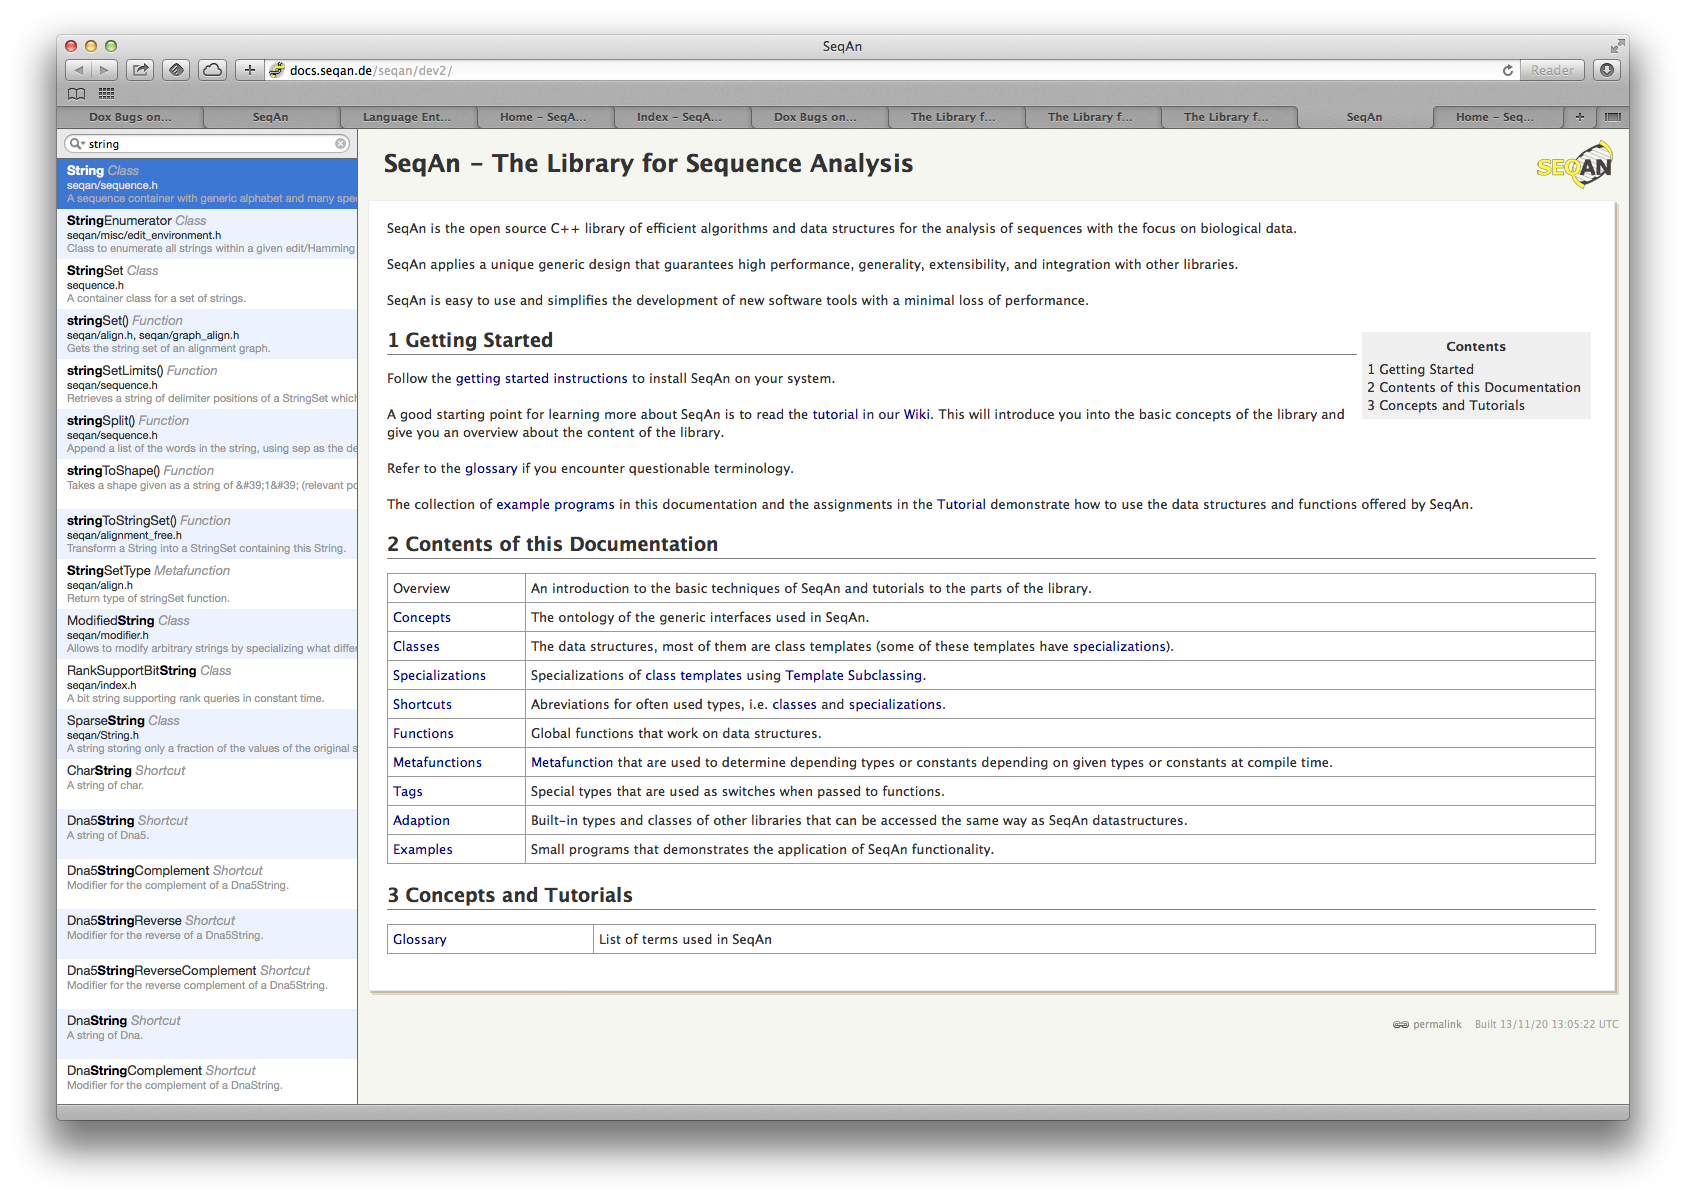
\includegraphics[width=\doxlargewidth]{Figures/dox/dox-2_0_0-large-string.png}
    \caption{Seqan-Online-Dokumentation in Version 2.0 - Breite Ansicht - Suche nach ``String''}
    \label{fig:dox-2_0_0-large-string}
\end{figure}

\begin{figure}
  \centering
    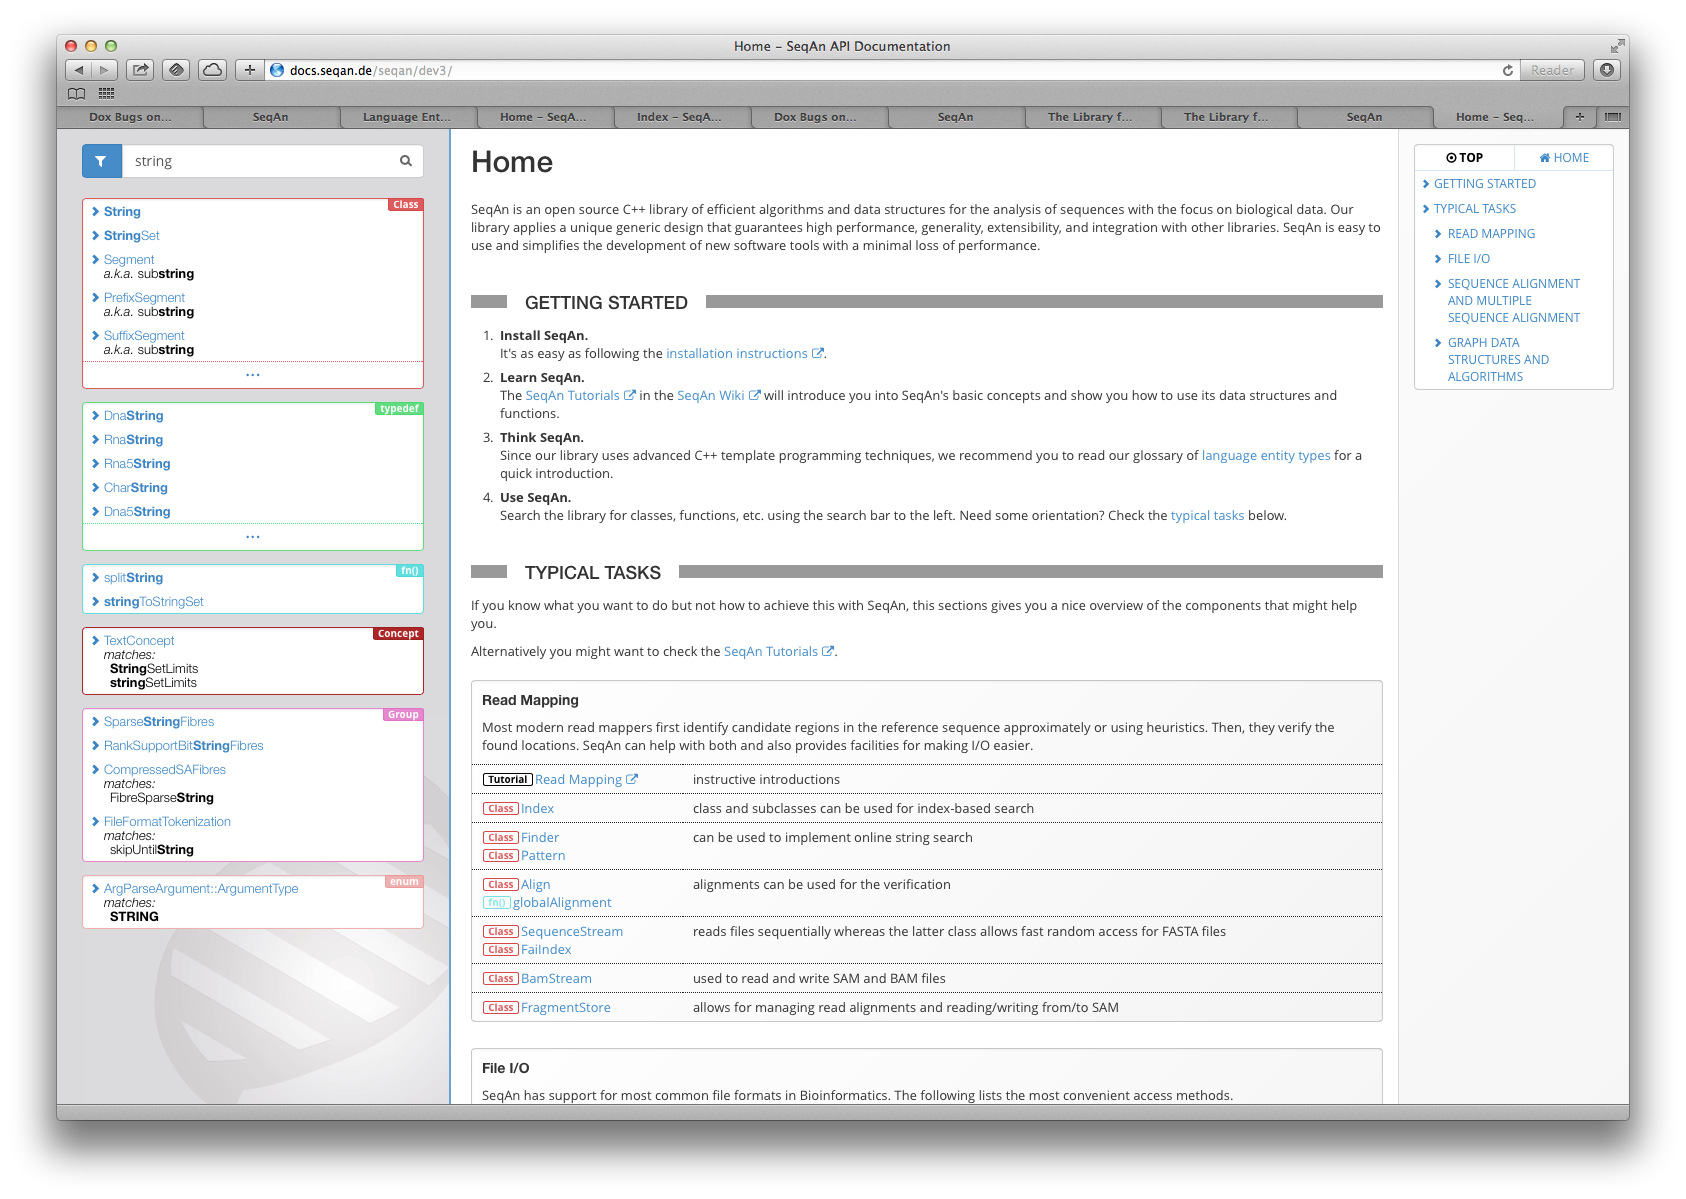
\includegraphics[width=\doxlargewidth]{Figures/dox/dox-3_0_0-large-string.png}
    \caption{Seqan-Online-Dokumentation in Version 3.0 - Breite Ansicht - Suche nach ``String''}
    \label{fig:dox-3_0_0-large-string}
\end{figure}

Donec urna leo, vulputate vitae porta eu, vehicula blandit libero. Phasellus eget massa et leo condimentum mollis. Nullam molestie, justo at pellentesque vulputate, sapien velit ornare diam, nec gravida lacus augue non diam. Integer mattis lacus id libero ultrices sit amet mollis neque molestie. Integer ut leo eget mi volutpat congue. Vivamus sodales, turpis id venenatis placerat, tellus purus adipiscing magna, eu aliquam nibh dolor id nibh. Pellentesque habitant morbi tristique senectus et netus et malesuada fames ac turpis egestas. Sed cursus convallis quam nec vehicula. Sed vulputate neque eget odio fringilla ac sodales urna feugiat.

\begin{figure}
  \centering
    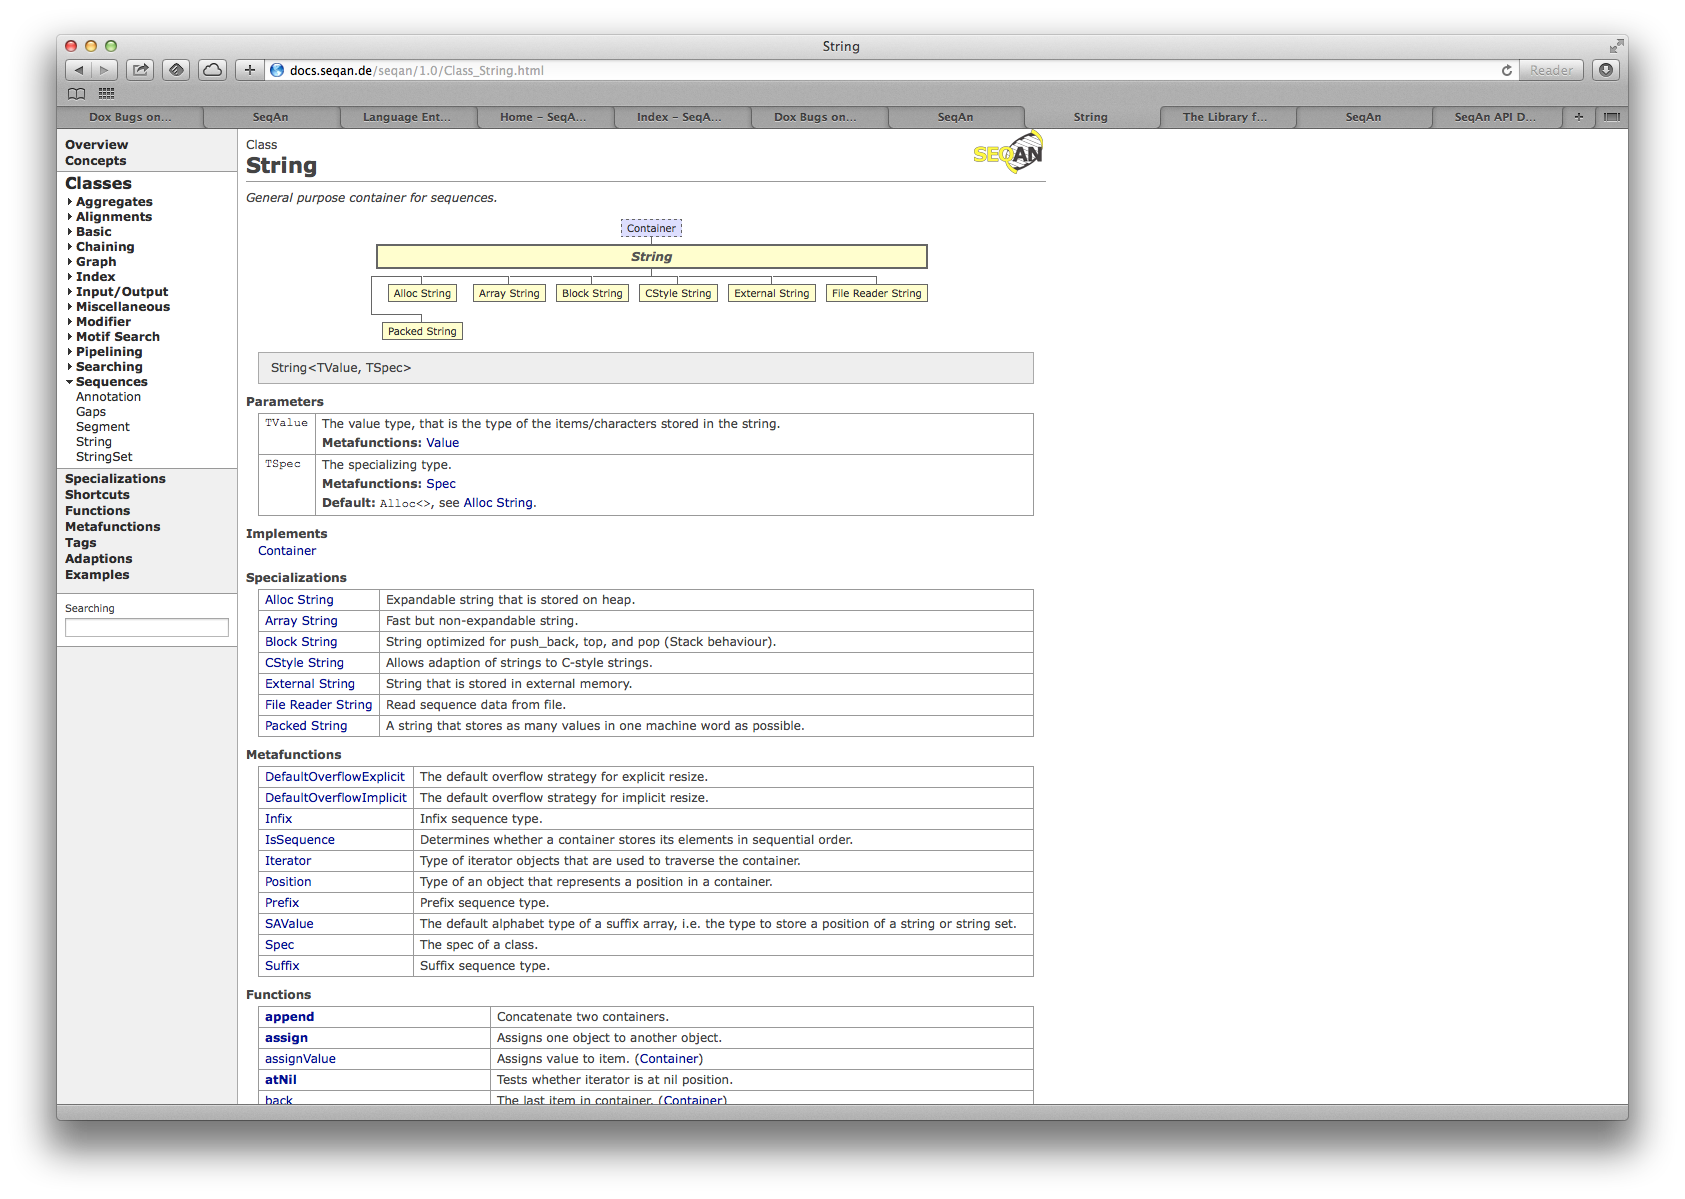
\includegraphics[width=\doxlargewidth]{Figures/dox/dox-1_0_0-large-string-opened.png}
    \caption{Seqan-Online-Dokumentation in Version 1.0 - Breite Ansicht - Klasse ``String''}
    \label{fig:dox-1_0_0-large-string-opened}
\end{figure}

\begin{figure}
  \centering
    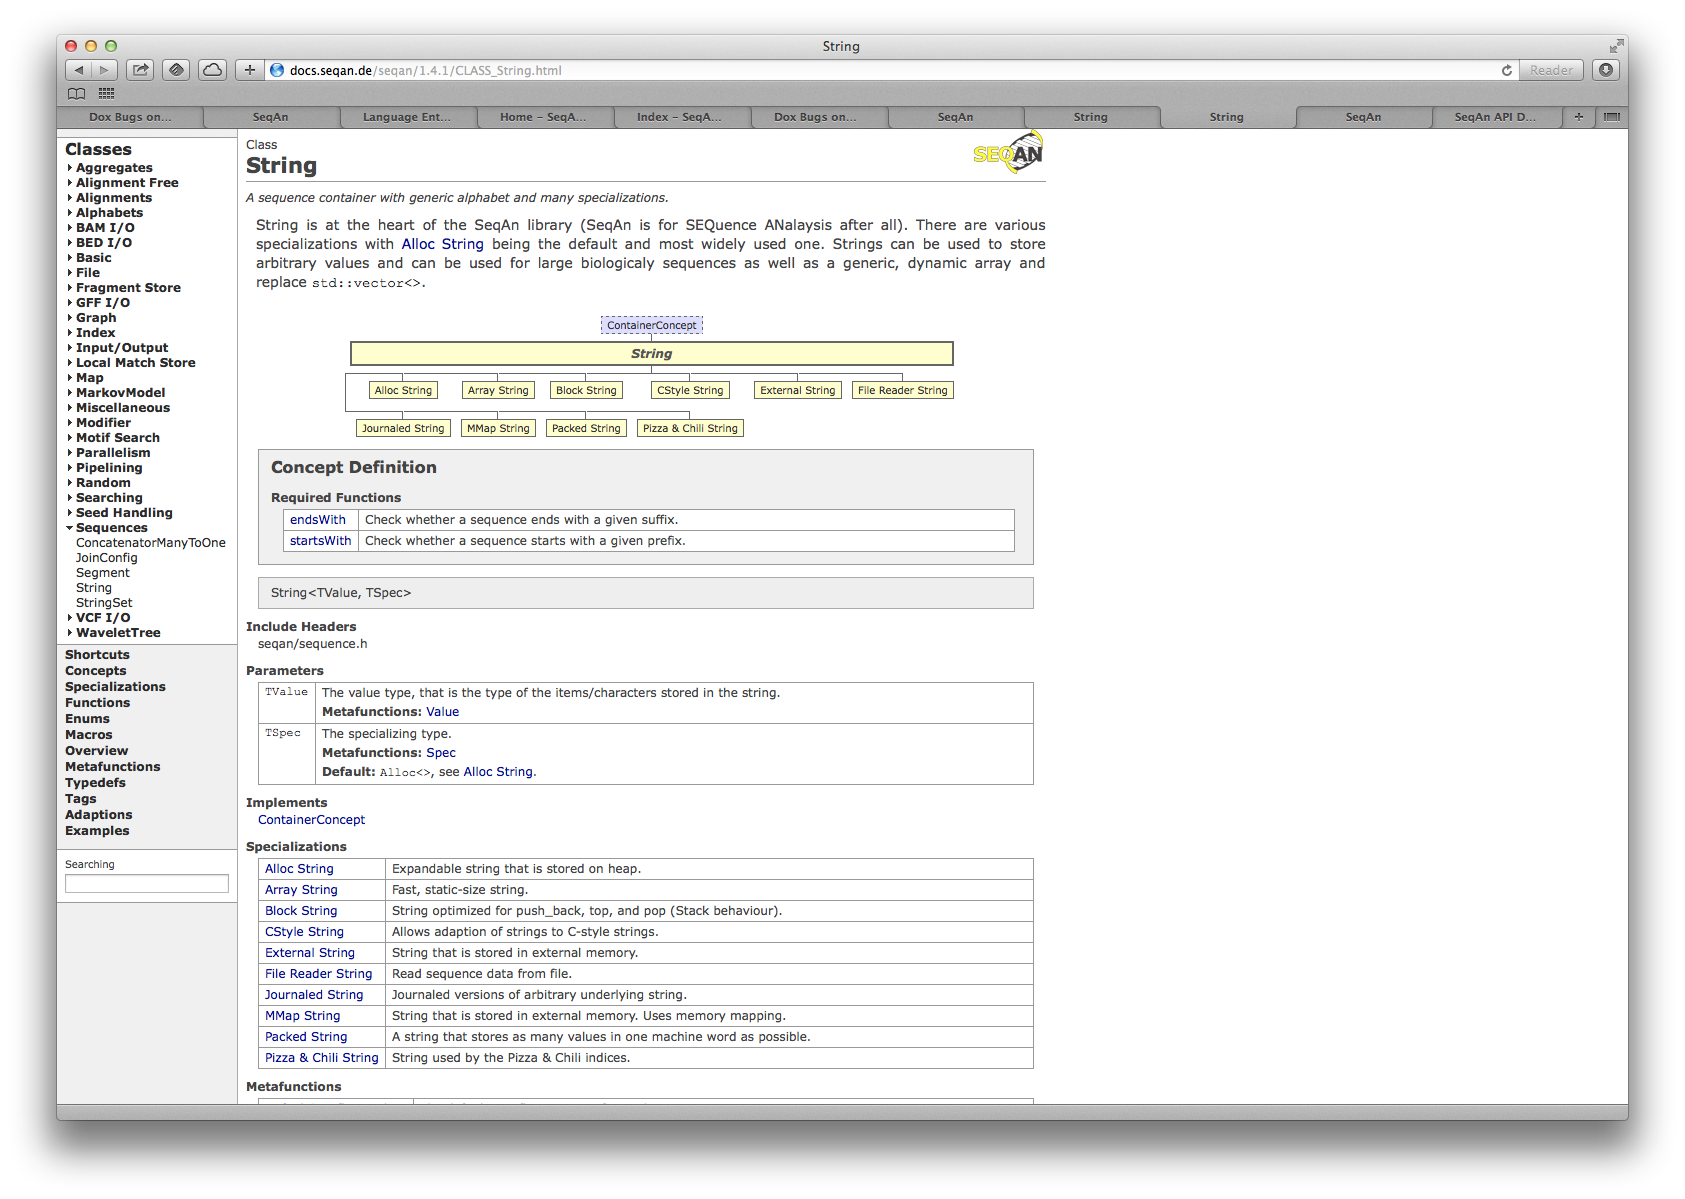
\includegraphics[width=\doxlargewidth]{Figures/dox/dox-1_4_1-large-string-opened.png}
    \caption{Seqan-Online-Dokumentation in Version 1.4.1 - Breite Ansicht - Klasse ``String''}
    \label{fig:dox-1_4_1-large-string-opened}
\end{figure}

Donec urna leo, vulputate vitae porta eu, vehicula blandit libero. Phasellus eget massa et leo condimentum mollis. Nullam molestie, justo at pellentesque vulputate, sapien velit ornare diam, nec gravida lacus augue non diam. Integer mattis lacus id libero ultrices sit amet mollis neque molestie. Integer ut leo eget mi volutpat congue. Vivamus sodales, turpis id venenatis placerat, tellus purus adipiscing magna, eu aliquam nibh dolor id nibh. Pellentesque habitant morbi tristique senectus et netus et malesuada fames ac turpis egestas. Sed cursus convallis quam nec vehicula. Sed vulputate neque eget odio fringilla ac sodales urna feugiat.

Donec urna leo, vulputate vitae porta eu, vehicula blandit libero. Phasellus eget massa et leo condimentum mollis. Nullam molestie, justo at pellentesque vulputate, sapien velit ornare diam, nec gravida lacus augue non diam. Integer mattis lacus id libero ultrices sit amet mollis neque molestie. Integer ut leo eget mi volutpat congue. Vivamus sodales, turpis id venenatis placerat, tellus purus adipiscing magna, eu aliquam nibh dolor id nibh. Pellentesque habitant morbi tristique senectus et netus et malesuada fames ac turpis egestas. Sed cursus convallis quam nec vehicula. Sed vulputate neque eget odio fringilla ac sodales urna feugiat.

\begin{figure}
  \centering
    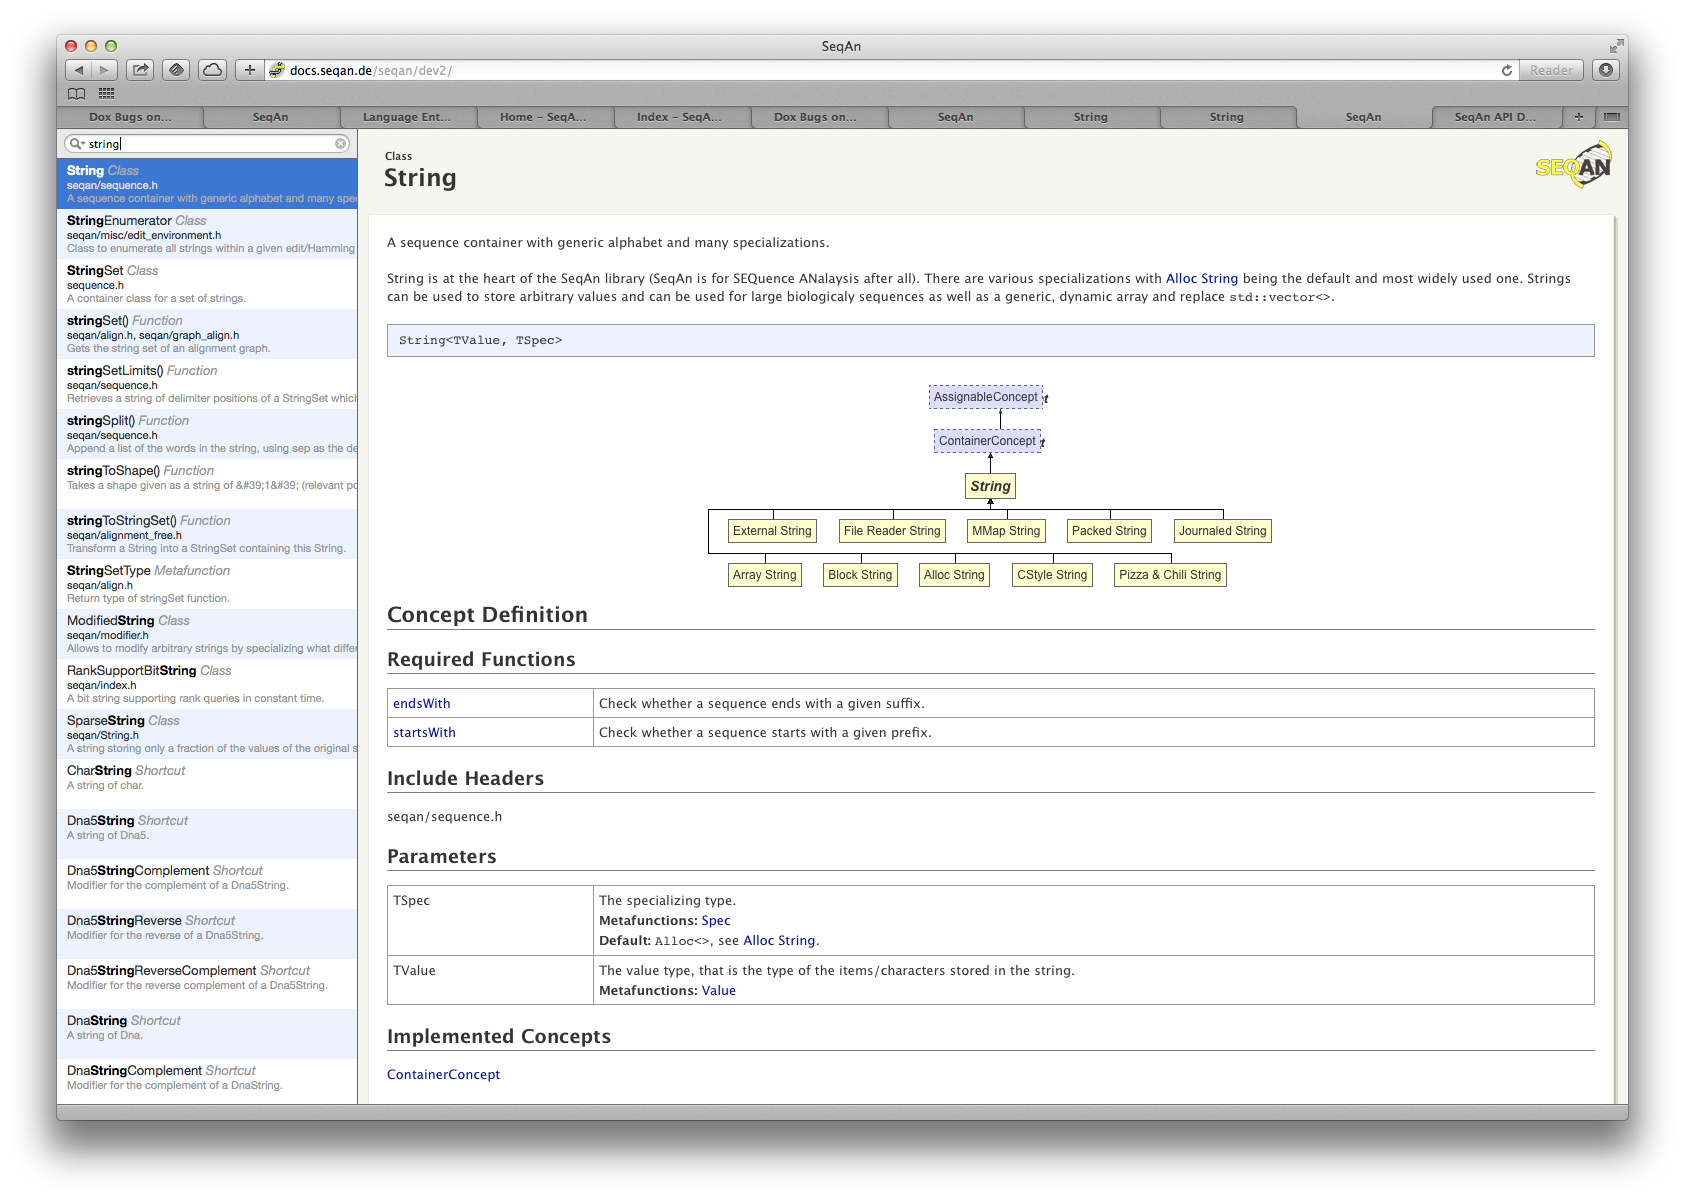
\includegraphics[width=\doxlargewidth]{Figures/dox/dox-2_0_0-large-string-opened.png}
    \caption{Seqan-Online-Dokumentation in Version 2.0 - Breite Ansicht - Klasse ``String''}
    \label{fig:dox-2_0_0-large-string-opened}
\end{figure}

\begin{figure}
  \centering
    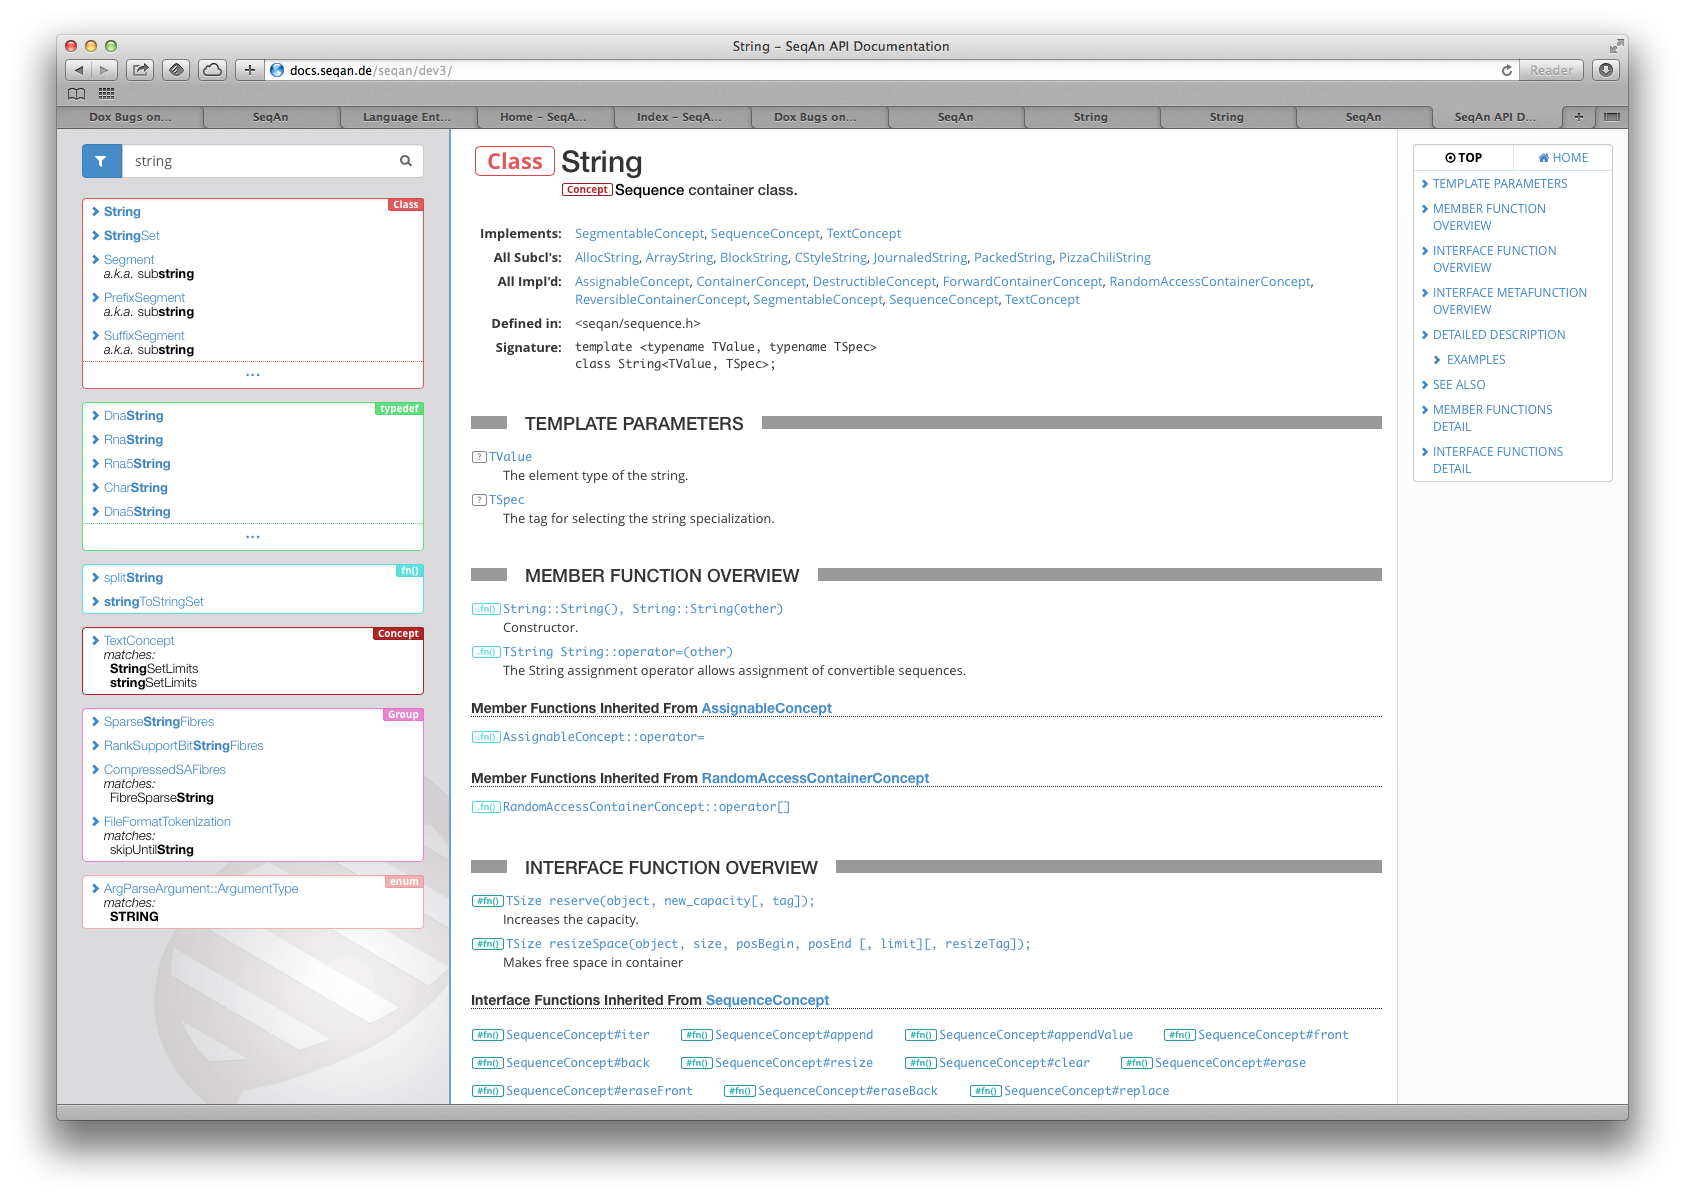
\includegraphics[width=\doxlargewidth]{Figures/dox/dox-3_0_0-large-string-opened.png}
    \caption{Seqan-Online-Dokumentation in Version 3.0 - Breite Ansicht - Klasse ``String''}
    \label{fig:dox-3_0_0-large-string-opened}
\end{figure}

Donec urna leo, vulputate vitae porta eu, vehicula blandit libero. Phasellus eget massa et leo condimentum mollis. Nullam molestie, justo at pellentesque vulputate, sapien velit ornare diam, nec gravida lacus augue non diam. Integer mattis lacus id libero ultrices sit amet mollis neque molestie. Integer ut leo eget mi volutpat congue. Vivamus sodales, turpis id venenatis placerat, tellus purus adipiscing magna, eu aliquam nibh dolor id nibh. Pellentesque habitant morbi tristique senectus et netus et malesuada fames ac turpis egestas. Sed cursus convallis quam nec vehicula. Sed vulputate neque eget odio fringilla ac sodales urna feugiat.

Donec urna leo, vulputate vitae porta eu, vehicula blandit libero. Phasellus eget massa et leo condimentum mollis. Nullam molestie, justo at pellentesque vulputate, sapien velit ornare diam, nec gravida lacus augue non diam. Integer mattis lacus id libero ultrices sit amet mollis neque molestie. Integer ut leo eget mi volutpat congue. Vivamus sodales, turpis id venenatis placerat, tellus purus adipiscing magna, eu aliquam nibh dolor id nibh. Pellentesque habitant morbi tristique senectus et netus et malesuada fames ac turpis egestas. Sed cursus convallis quam nec vehicula. Sed vulputate neque eget odio fringilla ac sodales urna feugiat.

\begin{figure}
  \centering
    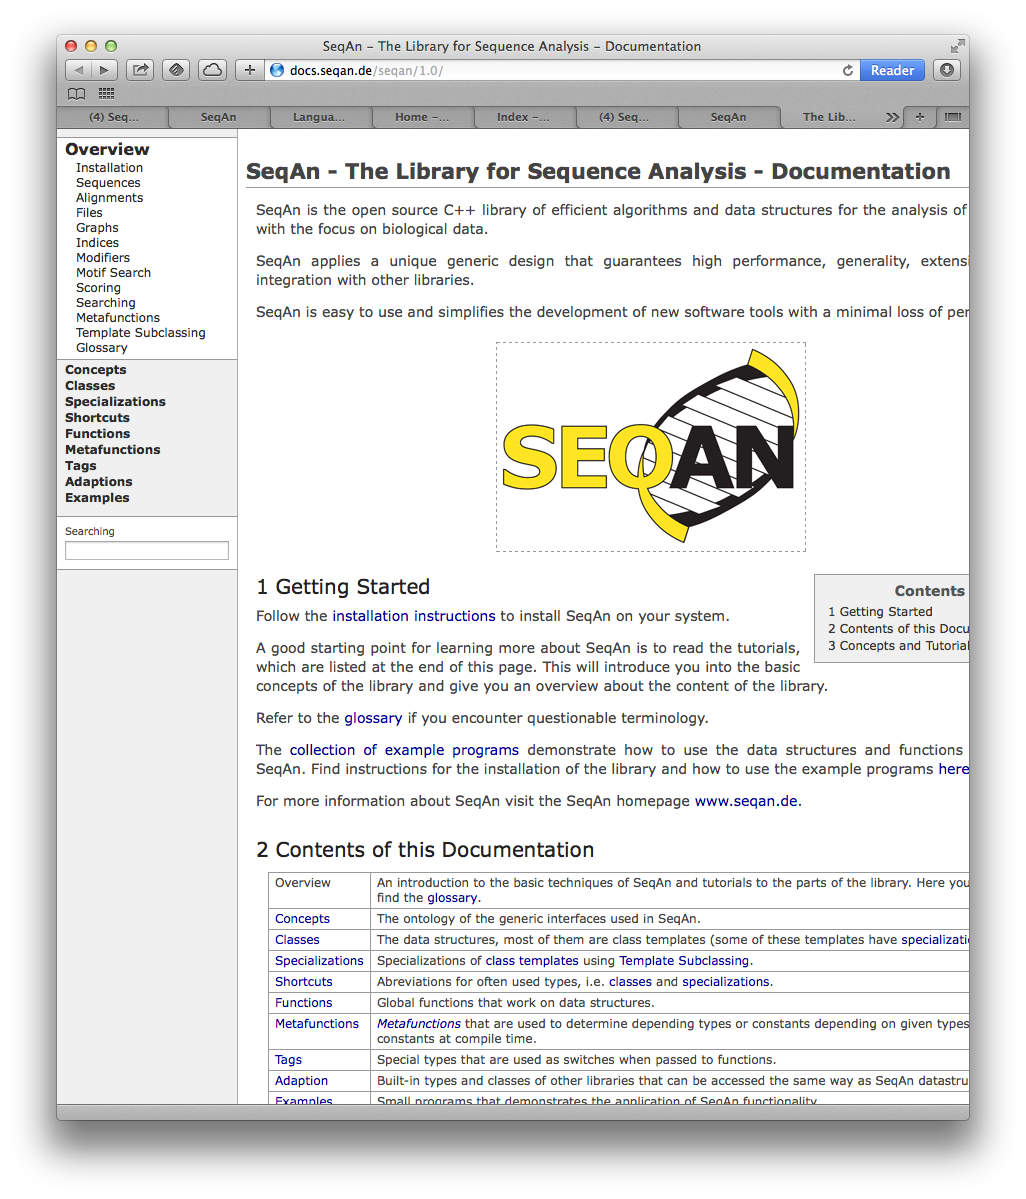
\includegraphics[width=\doxnarrowwidth]{Figures/dox/dox-1_0_0-small-home.png}
    \caption{Seqan-Online-Dokumentation in Version 1.0 - Smale Ansicht - Startseite}
    \label{fig:dox-1_0_0-small-home}
\end{figure}

\begin{figure}
  \centering
    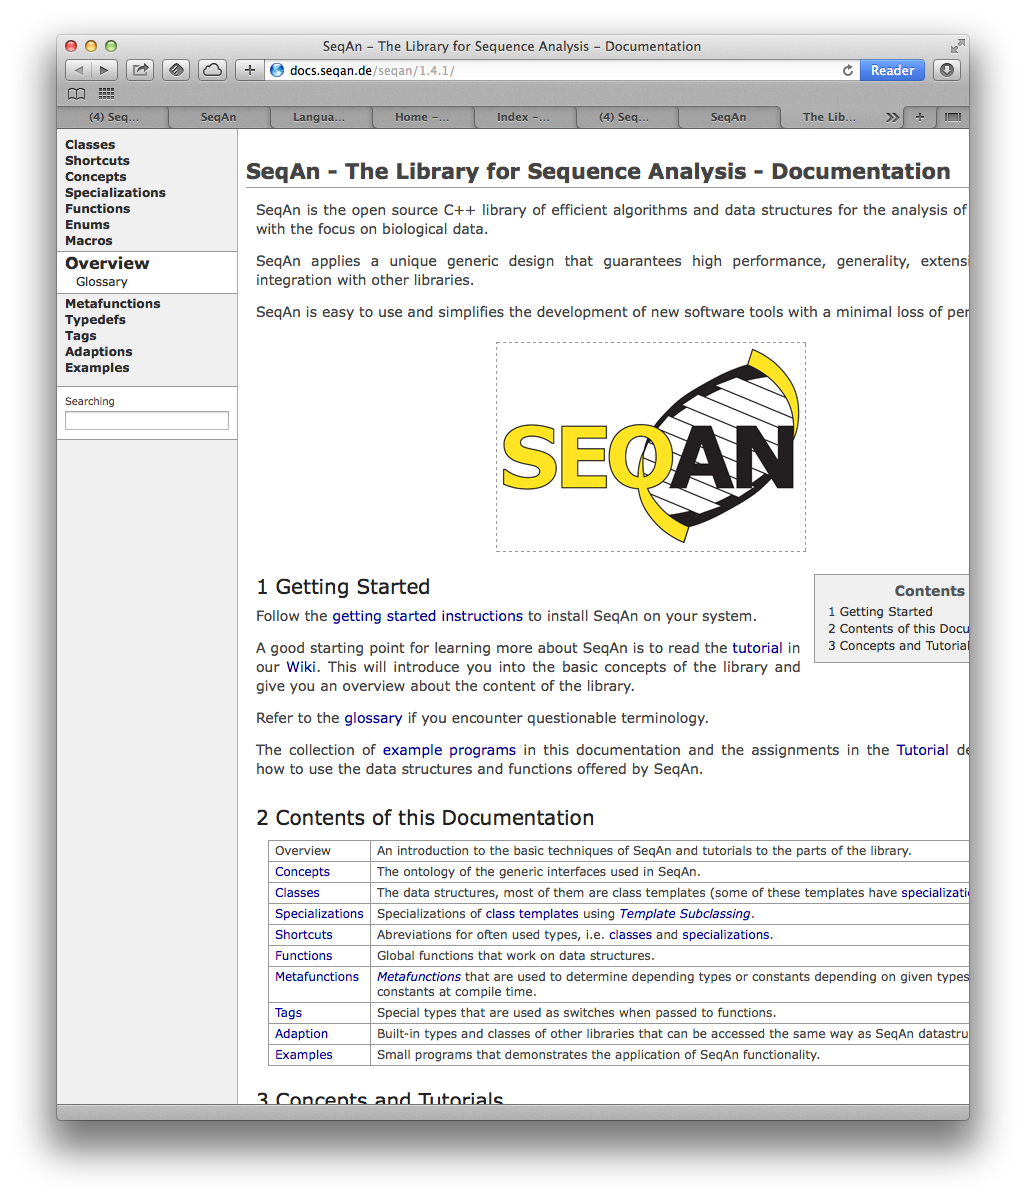
\includegraphics[width=\doxnarrowwidth]{Figures/dox/dox-1_4_1-small-home.png}
    \caption{Seqan-Online-Dokumentation in Version 1.4.1 - Smale Ansicht - Startseite}
    \label{fig:dox-1_4_1-small-home}
\end{figure}

\begin{figure}
  \centering
    \includegraphics[width=\doxnarrowwidth]{Figures/dox/dox-2_0_0-small-home.png}
    \caption{Seqan-Online-Dokumentation in Version 2.0 - Smale Ansicht - Startseite}
    \label{fig:dox-2_0_0-small-home}
\end{figure}

\begin{figure}
  \centering
    \includegraphics[width=\doxnarrowwidth]{Figures/dox/dox-3_0_0-small-home.png}
    \caption{Seqan-Online-Dokumentation in Version 3.0 - Smale Ansicht - Startseite}
    \label{fig:dox-3_0_0-small-home}
\end{figure}

Donec urna leo, vulputate vitae porta eu, vehicula blandit libero. Phasellus eget massa et leo condimentum mollis. Nullam molestie, justo at pellentesque vulputate, sapien velit ornare diam, nec gravida lacus augue non diam. Integer mattis lacus id libero ultrices sit amet mollis neque molestie. Integer ut leo eget mi volutpat congue. Vivamus sodales, turpis id venenatis placerat, tellus purus adipiscing magna, eu aliquam nibh dolor id nibh. Pellentesque habitant morbi tristique senectus et netus et malesuada fames ac turpis egestas. Sed cursus convallis quam nec vehicula. Sed vulputate neque eget odio fringilla ac sodales urna feugiat.

Donec urna leo, vulputate vitae porta eu, vehicula blandit libero. Phasellus eget massa et leo condimentum mollis. Nullam molestie, justo at pellentesque vulputate, sapien velit ornare diam, nec gravida lacus augue non diam. Integer mattis lacus id libero ultrices sit amet mollis neque molestie. Integer ut leo eget mi volutpat congue. Vivamus sodales, turpis id venenatis placerat, tellus purus adipiscing magna, eu aliquam nibh dolor id nibh. Pellentesque habitant morbi tristique senectus et netus et malesuada fames ac turpis egestas. Sed cursus convallis quam nec vehicula. Sed vulputate neque eget odio fringilla ac sodales urna feugiat.


\begin{figure}
  \centering
    \includegraphics[width=\doxnarrowwidth]{Figures/dox/dox-1_0_0-small-string.png}
    \caption{Seqan-Online-Dokumentation in Version 1.0 - Smale Ansicht - Suche nach ``String''}
    \label{fig:dox-1_0_0-small-string}
\end{figure}

\begin{figure}
  \centering
    \includegraphics[width=\doxnarrowwidth]{Figures/dox/dox-1_4_1-small-string.png}
    \caption{Seqan-Online-Dokumentation in Version 1.4.1 - Smale Ansicht - Suche nach ``String''}
    \label{fig:dox-1_4_1-small-string}
\end{figure}

\begin{figure}
  \centering
    \includegraphics[width=\doxnarrowwidth]{Figures/dox/dox-2_0_0-small-string.png}
    \caption{Seqan-Online-Dokumentation in Version 2.0 - Smale Ansicht - Suche nach ``String''}
    \label{fig:dox-2_0_0-small-string}
\end{figure}

\begin{figure}
  \centering
    \includegraphics[width=\doxnarrowwidth]{Figures/dox/dox-3_0_0-small-string.png}
    \caption{Seqan-Online-Dokumentation in Version 3.0 - Smale Ansicht - Suche nach ``String''}
    \label{fig:dox-3_0_0-small-string}
\end{figure}

Donec urna leo, vulputate vitae porta eu, vehicula blandit libero. Phasellus eget massa et leo condimentum mollis. Nullam molestie, justo at pellentesque vulputate, sapien velit ornare diam, nec gravida lacus augue non diam. Integer mattis lacus id libero ultrices sit amet mollis neque molestie. Integer ut leo eget mi volutpat congue. Vivamus sodales, turpis id venenatis placerat, tellus purus adipiscing magna, eu aliquam nibh dolor id nibh. Pellentesque habitant morbi tristique senectus et netus et malesuada fames ac turpis egestas. Sed cursus convallis quam nec vehicula. Sed vulputate neque eget odio fringilla ac sodales urna feugiat.

Donec urna leo, vulputate vitae porta eu, vehicula blandit libero. Phasellus eget massa et leo condimentum mollis. Nullam molestie, justo at pellentesque vulputate, sapien velit ornare diam, nec gravida lacus augue non diam. Integer mattis lacus id libero ultrices sit amet mollis neque molestie. Integer ut leo eget mi volutpat congue. Vivamus sodales, turpis id venenatis placerat, tellus purus adipiscing magna, eu aliquam nibh dolor id nibh. Pellentesque habitant morbi tristique senectus et netus et malesuada fames ac turpis egestas. Sed cursus convallis quam nec vehicula. Sed vulputate neque eget odio fringilla ac sodales urna feugiat.

\begin{figure}
  \centering
    \includegraphics[width=\doxnarrowwidth]{Figures/dox/dox-1_0_0-small-string-opened.png}
    \caption{Seqan-Online-Dokumentation in Version 1.0 - Smale Ansicht - Klasse ``String''}
    \label{fig:dox-1_0_0-small-string-opened}
\end{figure}

\begin{figure}
  \centering
    \includegraphics[width=\doxnarrowwidth]{Figures/dox/dox-1_4_1-small-string-opened.png}
    \caption{Seqan-Online-Dokumentation in Version 1.4.1 - Smale Ansicht - Klasse ``String''}
    \label{fig:dox-1_4_1-small-string-opened}
\end{figure}

\begin{figure}
  \centering
    \includegraphics[width=\doxnarrowwidth]{Figures/dox/dox-2_0_0-small-string-opened.png}
    \caption{Seqan-Online-Dokumentation in Version 2.0 - Smale Ansicht - Klasse ``String''}
    \label{fig:dox-2_0_0-small-string-opened}
\end{figure}

\begin{figure}
  \centering
    \includegraphics[width=\doxnarrowwidth]{Figures/dox/dox-3_0_0-small-string-opened.png}
    \caption{Seqan-Online-Dokumentation in Version 3.0 - Smale Ansicht - Klasse ``String''}
    \label{fig:dox-3_0_0-small-string-opened}
\end{figure}








Donec urna leo, vulputate vitae porta eu, vehicula blandit libero. Phasellus eget massa et leo condimentum mollis. Nullam molestie, justo at pellentesque vulputate, sapien velit ornare diam, nec gravida lacus augue non diam. Integer mattis lacus id libero ultrices sit amet mollis neque molestie. Integer ut leo eget mi volutpat congue. Vivamus sodales, turpis id venenatis placerat, tellus purus adipiscing magna, eu aliquam nibh dolor id nibh. Pellentesque habitant morbi tristique senectus et netus et malesuada fames ac turpis egestas. Sed cursus convallis quam nec vehicula. Sed vulputate neque eget odio fringilla ac sodales urna feugiat.

\newgeometry{inner=2cm,outer=1.5cm,top=1.5cm,bottom=1.5cm}
\thispagestyle{empty}
\begin{landscape}
\begin{figure}
        \centering
        \begin{subfigure}[b]{0.38\linewidth}
                \includegraphics[width=\linewidth]{Figures/dox/dox-1_0_0-large-home.png}
                \caption{Version 1.0.0}
                \label{fig:dox-large-home-1.0.0}
        \end{subfigure}
        \hspace{1cm}
        \begin{subfigure}[b]{0.38\linewidth}
                \includegraphics[width=\linewidth]{Figures/dox/dox-1_4_1-large-home.png}
                \caption{Version 1.4.1}
                \label{fig:dox-large-home-1.4.1}
        \end{subfigure}%
        \vskip\baselineskip
        \begin{subfigure}[b]{0.38\linewidth}
                \includegraphics[width=\linewidth]{Figures/dox/dox-2_0_0-large-home.png}
                \caption{Version 2.0.0}
                \label{fig:dox-large-home-2.0.0}
        \end{subfigure}
        \hspace{1cm}
        \begin{subfigure}[b]{0.38\linewidth}
                \includegraphics[width=\linewidth]{Figures/dox/dox-3_0_0-large-home.png}
                \caption{Version 3.0.0}
                \label{fig:dox-large-home-3.0.0}
        \end{subfigure}
        \caption{Diese Abbildung zeigt die verschiedenen Online-Dokumentation-Versionen mit ihrer Startseite.}
        \label{fig:dox-large-home-all}
\end{figure}
\end{landscape}
\restoregeometry

\newgeometry{inner=2cm,outer=1cm,top=1.5cm,bottom=1.5cm}
\thispagestyle{empty}
%\begin{landscape}
\begin{figure}
        \centering
        \begin{subfigure}[b]{0.48\linewidth}
                \includegraphics[width=\linewidth]{Figures/dox/dox-1_0_0-small-home.png}
                \caption{Version 1.0.0}
                \label{fig:dox-small-home-1.0.0}
        \end{subfigure}
        \hfill
        \begin{subfigure}[b]{0.48\linewidth}
                \includegraphics[width=\linewidth]{Figures/dox/dox-1_4_1-small-home.png}
                \caption{Version 1.4.1}
                \label{fig:dox-small-home-1.4.1}
        \end{subfigure}%
        \vskip\baselineskip
        \begin{subfigure}[b]{0.48\linewidth}
                \includegraphics[width=\linewidth]{Figures/dox/dox-2_0_0-small-home.png}
                \caption{Version 2.0.0}
                \label{fig:dox-small-home-2.0.0}
        \end{subfigure}
        \hfill
        \begin{subfigure}[b]{0.48\linewidth}
                \includegraphics[width=\linewidth]{Figures/dox/dox-3_0_0-small-home.png}
                \caption{Version 3.0.0}
                \label{fig:dox-small-home-3.0.0}
        \end{subfigure}
        \caption{Diese Abbildung zeigt die verschiedenen Online-Dokumentation-Versionen in schmaler Breiter mit ihrer Startseite.}
        \label{fig:dox-small-home-all}
\end{figure}
%\end{landscape}
\restoregeometry

Donec urna leo, vulputate vitae porta eu, vehicula blandit libero. Phasellus eget massa et leo condimentum mollis. Nullam molestie, justo at pellentesque vulputate, sapien velit ornare diam, nec gravida lacus augue non diam. Integer mattis lacus id libero ultrices sit amet mollis neque molestie. Integer ut leo eget mi volutpat congue. Vivamus sodales, turpis id venenatis placerat, tellus purus adipiscing magna, eu aliquam nibh dolor id nibh. Pellentesque habitant morbi tristique senectus et netus et malesuada fames ac turpis egestas. Sed cursus convallis quam nec vehicula. Sed vulputate neque eget odio fringilla ac sodales urna feugiat.

\newgeometry{inner=2cm,outer=1.5cm,top=1.5cm,bottom=1.5cm}
\thispagestyle{empty}
\begin{landscape}
\begin{figure}
        \centering
        \begin{subfigure}[b]{0.38\linewidth}
                \includegraphics[width=\linewidth]{Figures/dox/dox-1_0_0-large-string.png}
                \caption{Version 1.0.0}
                \label{fig:dox-large-string-1.0.0}
        \end{subfigure}
        \hspace{1cm}
        \begin{subfigure}[b]{0.38\linewidth}
                \includegraphics[width=\linewidth]{Figures/dox/dox-1_4_1-large-string.png}
                \caption{Version 1.4.1}
                \label{fig:dox-large-string-1.4.1}
        \end{subfigure}%
        \vskip\baselineskip
        \begin{subfigure}[b]{0.38\linewidth}
                \includegraphics[width=\linewidth]{Figures/dox/dox-2_0_0-large-string.png}
                \caption{Version 2.0.0}
                \label{fig:dox-large-string-2.0.0}
        \end{subfigure}
        \hspace{1cm}
        \begin{subfigure}[b]{0.38\linewidth}
                \includegraphics[width=\linewidth]{Figures/dox/dox-3_0_0-large-string.png}
                \caption{Version 3.0.0}
                \label{fig:dox-large-string-3.0.0}
        \end{subfigure}
        \caption{Diese Abbildung zeigt die verschiedenen Online-Dokumentation-Versionen mit dem Suchbegriff ``String''.}
        \label{fig:dox-large-string-all}
\end{figure}
\end{landscape}
\restoregeometry

\newgeometry{inner=2cm,outer=1cm,top=1.5cm,bottom=1.5cm}
\thispagestyle{empty}
%\begin{landscape}
\begin{figure}
        \centering
        \begin{subfigure}[b]{0.48\linewidth}
                \includegraphics[width=\linewidth]{Figures/dox/dox-1_0_0-small-string.png}
                \caption{Version 1.0.0}
                \label{fig:dox-small-string-1.0.0}
        \end{subfigure}
        \hfill
        \begin{subfigure}[b]{0.48\linewidth}
                \includegraphics[width=\linewidth]{Figures/dox/dox-1_4_1-small-string.png}
                \caption{Version 1.4.1}
                \label{fig:dox-small-string-1.4.1}
        \end{subfigure}%
        \vskip\baselineskip
        \begin{subfigure}[b]{0.48\linewidth}
                \includegraphics[width=\linewidth]{Figures/dox/dox-2_0_0-small-string.png}
                \caption{Version 2.0.0}
                \label{fig:dox-small-string-2.0.0}
        \end{subfigure}
        \hfill
        \begin{subfigure}[b]{0.48\linewidth}
                \includegraphics[width=\linewidth]{Figures/dox/dox-3_0_0-small-string.png}
                \caption{Version 3.0.0}
                \label{fig:dox-small-string-3.0.0}
        \end{subfigure}
        \caption{Diese Abbildung zeigt die verschiedenen Online-Dokumentation-Versionen in schmaler Breiter mit dem Suchbegriff ``String''.}
        \label{fig:dox-small-string-all}
\end{figure}
%\end{landscape}
\restoregeometry

Donec urna leo, vulputate vitae porta eu, vehicula blandit libero. Phasellus eget massa et leo condimentum mollis. Nullam molestie, justo at pellentesque vulputate, sapien velit ornare diam, nec gravida lacus augue non diam. Integer mattis lacus id libero ultrices sit amet mollis neque molestie. Integer ut leo eget mi volutpat congue. Vivamus sodales, turpis id venenatis placerat, tellus purus adipiscing magna, eu aliquam nibh dolor id nibh. Pellentesque habitant morbi tristique senectus et netus et malesuada fames ac turpis egestas. Sed cursus convallis quam nec vehicula. Sed vulputate neque eget odio fringilla ac sodales urna feugiat.

\newgeometry{inner=2cm,outer=1.5cm,top=1.5cm,bottom=1.5cm}
\thispagestyle{empty}
\begin{landscape}
\begin{figure}
        \centering
        \begin{subfigure}[b]{0.38\linewidth}
                \includegraphics[width=\linewidth]{Figures/dox/dox-1_0_0-large-string-opened.png}
                \caption{Version 1.0.0}
                \label{fig:dox-large-string-opened-1.0.0}
        \end{subfigure}
        \hspace{1cm}
        \begin{subfigure}[b]{0.38\linewidth}
                \includegraphics[width=\linewidth]{Figures/dox/dox-1_4_1-large-string-opened.png}
                \caption{Version 1.4.1}
                \label{fig:dox-large-string-opened-1.4.1}
        \end{subfigure}%
        \vskip\baselineskip
        \begin{subfigure}[b]{0.38\linewidth}
                \includegraphics[width=\linewidth]{Figures/dox/dox-2_0_0-large-string-opened.png}
                \caption{Version 2.0.0}
                \label{fig:dox-large-string-opened-2.0.0}
        \end{subfigure}
        \hspace{1cm}
        \begin{subfigure}[b]{0.38\linewidth}
                \includegraphics[width=\linewidth]{Figures/dox/dox-3_0_0-large-string-opened.png}
                \caption{Version 3.0.0}
                \label{fig:dox-large-string-opened-3.0.0}
        \end{subfigure}
        \caption{Diese Abbildung zeigt die verschiedenen Online-Dokumentation-Versionen mit der geöffneten Klasse \textit{String}.}
        \label{fig:dox-large-string-opened-all}
\end{figure}
\end{landscape}
\restoregeometry

\newgeometry{inner=2cm,outer=1cm,top=1.5cm,bottom=1.5cm}
\thispagestyle{empty}
%\begin{landscape}
\begin{figure}
        \centering
        \begin{subfigure}[b]{0.48\linewidth}
                \includegraphics[width=\linewidth]{Figures/dox/dox-1_0_0-small-string-opened.png}
                \caption{Version 1.0.0}
                \label{fig:dox-small-string-opened-1.0.0}
        \end{subfigure}
        \hfill
        \begin{subfigure}[b]{0.48\linewidth}
                \includegraphics[width=\linewidth]{Figures/dox/dox-1_4_1-small-string-opened.png}
                \caption{Version 1.4.1}
                \label{fig:dox-small-string-opened-1.4.1}
        \end{subfigure}%
        \vskip\baselineskip
        \begin{subfigure}[b]{0.48\linewidth}
                \includegraphics[width=\linewidth]{Figures/dox/dox-2_0_0-small-string-opened.png}
                \caption{Version 2.0.0}
                \label{fig:dox-small-string-opened-2.0.0}
        \end{subfigure}
        \hfill
        \begin{subfigure}[b]{0.48\linewidth}
                \includegraphics[width=\linewidth]{Figures/dox/dox-3_0_0-small-string-opened.png}
                \caption{Version 3.0.0}
                \label{fig:dox-small-string-opened-3.0.0}
        \end{subfigure}
        \caption{Diese Abbildung zeigt die verschiedenen Online-Dokumentation-Versionen in schmaler Breiter mit der geöffneten Klasse \textit{String}.}
        \label{fig:dox-small-string-opened-all}
\end{figure}
%\end{landscape}
\restoregeometry
\end{comment}


\subsection{Kollaborationsplattform}

Im Zuge der Umstellung des Versionsverwaltungssystems von Subversion auf Git wurde von einer selbst gehosteten Lösung auf \textit{GitHub}\footnote{\url{https://github.com}} umgestellt. Diese Plattform bietet einen \textit{Issue-Tracker}\footnote{\url{https://github.com/seqan/seqan/issues}}, der von SeqAn-Anwendern sehr gut angenommen und von SeqAn-Entwicklern aktiv verwaltet wird. Auf dieser Plattform findet ein fruchtbarer Austausch zwischen Anwendern und Entwicklern statt\footnote{Beispiel: \url{https://github.com/seqan/seqan/issues/919}}. 


\begin{comment}
\subsection{Werkzeugunterstützung}

Den Algorithmus zur automatischen Erzeugung von Code-Beispielen von \cite{Buse:2012vv} habe ich aus Zeitgründen nicht den SeqAn-Entwicklern vorstellig machen können.
\end{comment}



\subsection{Usability-Priorisierung}

Die gesamtheitliche Erforschung der Entwicklung der SeqAn-Library brachte erst spät die trivial erscheinende Erkenntnis, dass es Gründe für die besondere Betonung der Performance gab und erst die kommerzielle Verbreiterung des SeqAn-Einsatzzweckes zu einer notwendigen Neugewichtung der Usability führt bzw. führen muss.

Mit dieser Arbeit liefere ich belastbare Argumente für meine Theorie, die dem SeqAn-Entwicklungsteam dabei helfen sollen, diesen Perspektivwechsel wahrzunehmen und eine verstärkte Betonung der Usability in Form von expliziten-empirischen Entwurfsentscheidungen zu fördern. Diese Einsicht auf Entwicklerseite würde mittelfristig zu einer ganzheitlichen Verbesserung der API-Usability von SeqAn führen.



\subsection{Zusammenfassung}

Für die Verbesserung der API-Usability von SeqAn haben die Bioinformatik-Arbeitsgruppe und ich umfangreiche Maßnahmen umgesetzt.

Neben den aus der ersten Verbesserungsiteration stammenden Prozessverbesserungen, konnten meine SeqAn-Kollegen und ich drei der vier wichtigsten Maßnahmen vollständig bearbeiten:
\begin{enumerate}
  \item SeqAn kann nun auch als Library verwendet werden, indem insbesondere Vorwärtsdeklarationen beseitigt wurden. So simpel dieser Punkt klingen mag, so fundamental war er auch für potentielle SeqAn-Anwender, die ihren bestehenden Build-Prozess nicht anpassen wollten oder konnten. 
  \item Die Dokumentation wurde technisch neu entwickelt und inhaltlich überarbeitet. Dazu wurde das neue Dokumentationsformat Dox entwickelt, ein Gesamtüberblick erarbeitet sowie Seitenaufbau, Beispiele, Suchfunktion, Darstellung und die Integration verbessert. Außerdem wurde das Konzept der Sprachentitätstypen gesamtheitlich innerhalb der Dokumentation implementiert. Ergänzt wird die Verbesserung der Dokumentation durch die bereits in der ersten Verbesserungsiteration generalüberholten Installationsanleitungen und Tutorials.
  \item SeqAn kann nun von API-Endanwendern genutzt werden. Dazu wurde eine Wrapper-API in Form einer Integration in die Workflow-Engine KNIME implementiert.% Zu diesem Zweck wurde ein neuer Argument-Parser entwickelt, der explizierte Schnittstellenbeschreibungen von SeqAn-Anwendungen in einem definierten Format ausgeben kann. Diese Beschreibungen dienen wiederum dem ebenfalls weiterentwickelten Generic Workflows Nodes Werkzeug als Eingabe zur Generierung von KNIME-Knoten, die ein automatisierter Prozess allen KNIME-Anwendern zur Verfügung stellt. 
\end{enumerate}

Außerdem abgeschlossen wurde die Einrichtung einer Kollaborationsplattform --- in Form eines GitHub Issue-Trackers --- für den Austausch zwischen SeqAn-Entwicklern und -Anwendern.

Aus diversen, insbesondere Zeitgründen konnte ich leider nicht darauf hinwirken, dass die wichtige STL-Angleichung in Angriff genommen wurde. Zwar sind Metafunktionen zur Berechnung von Rückgabetypen, wegen des in C\texttt{++}11 eingeführten \texttt{auto}-Schlüsselworts theoretisch nicht mehr nötig, was die mit dieser Maßnahme in Verbindung stehenden Usability-Probleme teilweise entschärft. Dies muss jedoch noch praktisch gezeigt werden. Im Erfolgsfall müssen außerdem sämtliche Lernressourcen entsprechend angepasst werden. Diese Entwicklung hat jedoch keinen Einfluss auf meine dringende Empfehlung, das CRTP einzusetzen, um die globalen Funktionen zu Memberfunktionen zu refaktorisieren, die auch in C\texttt{++} als Memberfunktionen implementiert sind.

Ebenfalls aus Zeitgründen konnten die Maßnahmen Inkonsistenzbeseitigung, Shortcuts und die Evaluation des Code-Beispiel-Erzeugungs-Algorithmus nicht umgesetzt werden.

Das dem der Maßnahme Intransparenzbeseitigung zu Grunde liegende Usability-Problem \code[apiua://code/-9223372036854775057]{versteckte Parameterübergabe} ist in Bezug auf seine Fatalität nicht hinreichend gut verstanden, weshalb ich die Umsetzung der Maßnahme angesichts der hohen Kosten momentan nicht empfehlen kann.

Die Umsetzung der abstrakten Maßnahme Usability-Priorisierung ist längst nicht abgeschlossen und soll durch diese Arbeit motiviert werden.

\section{Güte, Validierung und Verallgemeinerbarkeit}
\label{sec:validierung}

In den vorangegangenen Unterkapiteln habe ich meine \gls{gt} vorgestellt. Für die darin beschriebenen Usability-Probleme habe ich Lösungsmaßnahmen vorgeschlagen und deren Bearbeitung durch die SeqAn-Entwickler beschrieben.

In diesem Unterkapitel möchte ich die Fragen beantworten, inwiefern meine Forschung überhaupt den Gütekriterien qualitativer Forschung entspricht und ob die Umsetzung meiner vorgeschlagenen Maßnahmen tatsächlich zu der erhofften Usability-Verbesserung führten. Des Weiteren möchte ich die Frage nach der Verallgemeinerbarkeit meiner Forschungsmethode und -ergebnisse klären.

\subsection{Güte}

In dieser Arbeit habe ich einen qualitativen Forschungsansatz gewählt, bei dem die \gls{gtm} eine große Rolle spielt. Für die Bewertung der Güte meiner Arbeit gelten also die am Anfang dieser Arbeit, im \sref{sec:gtm}, vorgestellten Gütekriterien qualitativer Forschung. Entlang dieser Gütekriterien werde ich meine Arbeit bewerten.

\begin{description}
  \item[Verfahrensdokumentation] \hfill \\
  Ich habe meine durch die wissenschaftliche Literaturstudie erworbenen Vorkenntnisse, die Forschungsplanung, die Datenerhebung, den Bau des Datenanalysewerkzeugs, die Herleitung der \gls{gt}, das Zustandekommen der Verbesserungsvorschläge und deren Umsetzung ausführlich beschrieben. Dabei habe ich die erhobenen Daten und die Grundlagen der von mir entwickelten Konzepte detailliert mittels entsprechender URIs zugänglich gemacht. Durch den Einsatz einer Versionsverwaltung kann sogar das Zustandekommen meiner als XML-Datei gesicherten Theorie über die Zeit nachvollzogen werden.
  
  \item[Argumentative Interpretationsabsicherung] \hfill \\
  Aus Platz-, Zeit- und Plausibilitätsgründen habe ich der Darstellung von Interpretationsalternativen nur wenig Raum in dieser Arbeit gegeben. Wenn es zu Konzepten relevante Literatur gab, habe ich diese genannt und zu meinen Beobachtungen in Beziehung gesetzt. Hatte ich Unsicherheiten in der Interpretation von Konzepten, habe ich diese bei für wichtig geglaubten Konzepten ausgeräumt. Weniger wichtige Konzepte habe ich in dieser Arbeit nicht aufgeführt. Die schlecht verstandenen Konzepte (z.B. \code[apiua://code/-9223372036854775057]{versteckte Parameterübergabe}) habe ich als solche deklariert.
  
  \item[Regelgeleitetheit] \hfill \\
  Meine Forschungsergebnisse entstanden innerhalb eines Prozesses, der stark durch die \gls{gtm} geprägt war. Durch die Implementierung eines dazugehörigen Analysewerkzeugs habe ich insbesondere die Phasen des offenen und axialen Kodierens und damit einen umfangreichen Prozessteil kodifiziert. Bei meiner Forschung kam es zu Abweichungen, die ich nachvollziehbar erläutert habe. Beispielsweise habe ich begründet, weshalb eine erste Beseitigung grober Usability-Probleme notwendig war und auf welche Weise ich dazu eine vereinfachte Form der \glslink{he}{Heuristischen Evaluation (HE)} durchgeführt habe. Weiterhin habe ich erläutert, dass ich eine besonders gründliche und breit aufgestellte Datenerhebung durchgeführt habe, um trotz der widrigen Umstände theoretischen Sampling durchführen zu können.
  
  \item[Nähe zum Gegenstand] \hfill \\
  Dank der Workshops, zu denen auch langjährige SeqAn-Anwender gehörten, konnte ich reale SeqAn-Anwender und die, die es möglicherweise werden wollten, beobachten. Meine Art der Datenaufzeichnung hat es mir erlaubt, auf ein Laborsetting zu verzichten, bei dem Anwender an ``unnatürlichen'', speziell für die Datenaufzeichnung vorbereiteten Arbeitsplätzen arbeiten müssten. Ich habe sowohl rein objektive Daten, als auch subjektive Daten erhoben. Für die Erhebung Letzterer habe ich zu den SeqAn-Anwendern ein gegenseitiges und offenes Verhältnis gepflegt und mein Arbeitsziel klar und ohne ``Täuschung'' formuliert. Auf diese Weise wurden den SeqAn-Anwendern deutlich, dass sie und ich ein gemeinsames Ziel verfolgen --- nämlich ein benutzerfreundliches SeqAn.
  Schwächen hatte meine Forschung bzgl. dieses Kriteriums, weil ich Anwender nicht an ihrem natürlichen Arbeitsplatz, sondern in Praktika und Workshops beobachtet habe. Meine Langzeitaufzeichnungen könnten diesen Punkt entkräften, jedoch habe ich für deren Analyse keine Zeit aufbringen können. 
  
  \item[Kommunikative Validierung] \hfill \\
  Die Gültigkeit vieler Ergebnisse --- insbesondere der \code{apiua://code/-9223372036854775633} --- konnte ich auf zwei Kommunikationswegen mit den SeqAn-Anwendern validieren. Einerseits zeigten die Datenerhebungen nach Überarbeitungen von SeqAn (z.B. Dokumentation) viel positives Feedback. Andererseits wurden Analyseergebnisse direkt mit SeqAn-Anwendern besprochen, wie dies beispielsweise bei der Gruppendiskussion der Fall war. Manche Ergebnisse konnte ich jedoch nicht validieren, weil mir entweder die Zeit fehlte oder ich die betroffene Person wegen meiner streng-pseudonymisierten Datenerhebung nicht identifizieren konnte (z.B. \code[apiua://code/-9223372036854775057]{versteckte Parameterübergabe}). Die Triangulation vieler meiner Ergebnisse mit existierender Literatur verbessert die Verallgemeinerbarkeit dieser Ergebnisse.
  
  \item[Triangulation] \hfill \\
  Für die Datenerhebung und -analyse kamen sowohl subjektive (Umfrage, Interview, Feedback, Gruppendiskussion und CDF-Fragebogen) als auch objektive Datenquellen (Programmierfortschritte) zum Einsatz (Datentriangulation). Für die Forschung selbst verwendete ich die \acrshort{he} und die \gls{gtm} (Methodentriangulation). Eine Reihe von Erkenntnissen konnte auf diese Weise trianguliert werden. Dabei traten in unterschiedlichen Datenquellen Konzepte mit unterschiedlichen Schwerpunkten auf (z.B. CDF-Fragebogen: \code{apiua://code/-9223372036854775280}; Gruppendiskussion: \code{apiua://code/-9223372036854775633}; Programmierfortschritte: \code{apiua://code/-9223372036854774904}).
  
  Aus Zeitgründen konnte ich leider den Großteil der sich aus den subjektiven Daten ergebenen Ergebnisse nicht mit Hilfe meiner Programmierfortschritte-Datenquelle validieren. Dennoch bin ich der festen Überzeugung, dass dies für viele Konzepte möglich ist. Besonders gut dafür geeignet sind die Daten meines Langzeitprobanden, da bei ihm nicht davon auszugehen ist, dass Beobachtungen auf fachlich schlechte Kenntnisse zurückzuführen sind. Die Auswertung dieser Daten bleibt nachfolgenden Arbeiten überlassen. 
  

  
%  Analyse der CDs (exklusiv: Kategorie \code{apiua://code/-9223372036854775237}
%  Funktionsblock, u.a. mit Unterkonzepten \code{apiua://code/-9223372036854775280} \code{apiua://code/-9223372036854775279})
%  Analyse der Gruppendiskussion (exklusiv: \code{piua://code/-9223372036854775633})
\end{description}

\bigskip

Im \sref{sec:gtm} habe ich neben den Gütekriterien nach \cite{mayring2002einfhrung} auch weitere Gütekriterien nach \cite{gesis-solis-00272267} vorgestellt, die sich zwar überschneiden, ich an dieser Stelle aber dennoch für die Bewertung meiner Arbeit heranziehen möchte:
\begin{description}
  \item[Intersubjektive Nachvollziehbarkeit] \hfill \\
  Meine Argumentation in Bezug auf die \textit{Verfahrensdokumentation} trifft auch auf dieses Gütekriterium zu.
   
  \item[Reflektierte Subjektivität] \hfill \\
  Während meiner Arbeit habe ich meine eigene Rolle als Bestandteil des Forschungsprozesses reflektiert, weshalb ich für meine Ausarbeitung auch die Ich-Form gewählt habe. Ich war mir bewusst, dass ich ein \gls{gtm}-Anfänger und zu Forschungsbeginn in keiner Weise mit der Bioinformatik vertraut war. Während ich Ersteres strukturiert, und, so gut es geht, ausgeräumt habe\footnote{Dazu habe ich auf die Erfahrungen meiner \gls{gtm}-geübten Kollegen zurückgegriffen,  viel \gls{gtm}-Literatur gelesen und eine einwöchige \gls{gtm}-Weiterbildung absolviert. Durch die Entwicklung eines qualitativen Analysewerkzeugs, habe ich mich besonders intensiv mit der \gls{gtm} auseinander gesetzt.}, hätte ich mich mit Letzterem intensiver --- z.B. durch den Besuch von Bioinformatik-Lehrveranstaltungen --- auseinandersetzen können. Meine Beschäftigung mit der Bioinformatik bestand hauptsächlich in der Teilnahme an Bioinformatik-Vorträgen und vielen Fragen an meine Bioinformatik-Kollegen. Probleme mit meinem Bioinformatik-Kenntnisstand konnte ich bei der Analyse der Programmierfortschritte-Daten feststellen, was die ohnehin zeitraubende Analyse weiter verlangsamte. Bei der Analyse subjektiver Daten fiel mir hingegen keinerlei Mangel auf. Auch wenn ich es bezweifle, kann ich abschließend nicht sagen, ob sich andere Theorieschwerpunkte ergeben hätten, hätte ich über bessere Bioinformatik-Kenntnisse verfügt.
  
  Meine Sensibilität für Usability ist interessenbedingt hoch. In Bezug auf API-Usability habe ich meine Sensibilität insbesondere durch die Durchführung der in dieser Arbeit vorgestellten, umfassenden Literaturforschung erhöht.
  
  Meine Nähe zu den SeqAn-Anwendern habe ich bereits unter dem Gütekriterium \textit{Nähe zum Gegenstand} erläutert.
%  Erfahrung im Einsatz der HE
%  GTM nach  \cite{strauss1990basics} und nicht nach \cite{glaser1978theoretical} verwendet, u.a. weil besser strukturierter Forschungsprozess besser für Anfänger

  \item[Limitation]\hfill \\
  Dieses Kriterium befasst sich mit den Grenzen der Verallgemeinerbarkeit der entwickelten Theorie, worauf ich im nächsten Abschnitt eingehe.
\end{description}

Auch wenn es nach meiner Kenntnis kein Gütekriterium \textit{Intrasubjektive Nachvollziehbarkeit} in der Literatur gibt, habe ich ein solches dennoch feststellen können. Mir fiel auf, dass meine Bewertungen einer Vielzahl von Phänomen und Konzepten immer wieder mit den vor Monaten bereits in Memos festgehaltenen Bewertungen weitgehend übereinstimmten. Dies deutet auf eine stabile Interpretation hin.




\subsection{Validierung}

In der ursprünglichen Planung (siehe \sref{sec:verlauf}) war vorgesehen, dass ich eine weitere Datenerhebung durchführe, die erhobenen Daten analysiere und prüfe, ob die vermeintlich behobenen Usability-Probleme tatsächlich zu einer API-Usability-Verbesserung beitrugen.

Dies war mir aus diversen Gründen (siehe \sref{sec:schwierigkeiten}) nicht möglich. Daher entschloss ich mich, eine vereinfachte Validierung mit Hilfe des Cognitive Dimension Frameworks durchzuführen.

\subsubsection{Validierung mit Hilfe des Cognitive Dimension Frameworks}
\label{sec:cdf-validation-difficulties}

Das Cognitive Dimensions Framework habe ich ausführlich im \sref{sec:cdf} vorgestellt. Um zumindest eine vereinfachte Validierung vorzunehmen, wollte ich den von mir entwickelten Cognitive-Dimension-Fragebogen (siehe \sref{sec:cdf-usage}) einmal vor und einmal nach der Umsetzung der von mir vorgeschlagenen Verbesserungsmaßnahmen einsetzen. Dafür hätte ich zwei Idealprofile --- eins für die SeqAn-Anwender und eins für die SeqAn-Endanwender --- erarbeiten müssen. Abweichungen der SeqAn-Profile vor und nach der Umsetzung der Maßnahmen würden dann mit den Anwender-bestimmten Idealprofilen verglichen werden müssen, um Aussagen über die Verbesserung treffen zu können.

Bedauerlicherweise scheiterte mein Versuch der Validierung mit Hilfe des CDF. Zum einen ist die konkrete Anwendung des CDF schlecht in \cite{AnIntroductiontot:1996ux} erklärt (siehe \sref{sec:cdf-application}). Des Weiteren wird kaum erläutert, wie das Idealprofil --- oder in meinem Fall die zwei Idealprofile --- zu ermitteln sind. Die Autoren empfehlen den Einsatz eines Fragebogens, der allerdings seine eigenen Probleme in sich birgt (siehe \sref{sec:cdf-usage}). Beispielsweise werden nicht alle Fragen hinreichend ausführlich beantwortet, weil der Fragebogen schlicht zu umfassend ist. Oder aber, Fragen werden von den Befragten falsch verstanden, wodurch man die entsprechende dimensionale Ausprägung nicht mehr belastbar bewerten kann, denn die dazu notwendigen Informationen liegen ja nicht vor. Diese Probleme führen dazu, dass weit mehr als zehn ausgefüllte Fragebögen notwendig sind, um jede kognitive Dimension valide einschätzen zu können.

Ein weiteres Problem ist, dass es Überlappungen und Abhängigkeiten zwischen den kognitiven Dimensionen gibt \citep{carroll2003hci}. Auch fehlt es in der Literatur an Studien, die das CDF tatsächlich vollständig eingesetzt hätten \citep[vgl.][]{carroll2003hci,roast2000formal,GreenCognitive}. Selbst der umfangreichste, von mir gefundene Anwendungsfall behandelt nur 6 der 14 Dimensionen \citep{GreenCognitive}. Da es sich bei der Bewertung der kognitiven Dimensionen jeweils um einen Einzelfall handelt, reicht diese Demonstration jedoch nicht aus, um die anderen kognitiven Dimensionen bewerten zu können.

Außerdem ist der Vergleich von zwei Profilen in Bezug auf eine kognitive Dimension schwierig, denn in der CDF-Literatur gibt es keinerlei Angaben dazu, wie Messungen quantitativ verglichen werden könnten.

\begin{comment}
\fref{fig:cd-validierungsversuch} zeigt meinen gescheiterten Versuch, das SeqAn-Profil aus meinen am Workshop'13 durchgeführten Cognitive-Dimensions-Fragebögen zu extrahieren.

\begin{figure}
  \centering
    \includegraphics[width=0.7\linewidth]{Figures/cd-validierungsversuch}
  \caption[Gescheiterter Validierungsversuch mittels CDF]{Gescheiterter Versuch der Erhebung des kognitiven Profils von SeqAn mittels Cognitive Dimensions Framework}
  \label{fig:cd-validierungsversuch}
\end{figure}
\end{comment}


\subsubsection{Argumentative Validierung}

Da ich weder eine empirische (siehe \sref{sec:schwierigkeiten}), noch eine verkürzte Validierung mittels CDF vornehmen konnte, bin ich dazu gezwungen, eine argumentative Validierung durchzuführen.

Was die Auswahl der Probanden betrifft, kann ich feststellen, dass die beobachteten SeqAn-Anwender die SeqAn-Anwenderschaft für meine Forschung hinreichend repräsentieren\footnote{In der ersten Analysephase habe ich die Anwenderschaft von SeqAn charakterisiert (siehe \sref{sec:results-users}). Zu dieser gehören berufstätige, nationale und internationale Wissenschaftler aus den Bereichen Informatik, Bioinformatik und Physik. Aus diesem Grund halte ich diese Personen geeignet als Probanden für meine Forschung. Der Studentenanteil stellt keine Probleme dar, da er einen beachtlichen Teil zur bioinformatischen Arbeit beiträgt \citep{Letondal:2006dy} und damit mindestens zur zukünftigen Anwendergruppe gerechnet werden kann.}, was wichtig für valide Ergebnisse ist \citep{Clarke:2004te,Henning:2007kg}. Lediglich, wenn einzelne Usability-Probleme besser hätten verstanden werden müssen, wäre eine zielgerichtetere Auswahl der Probanden und eine langfristigere Beobachtung notwendig gewesen. Die wenigen Usability-Probleme, die ich nicht ausreichend verstanden habe, habe ich auch als solche benannt.

%Für die Validität meiner ab Seite \pageref{sec:gt} vorgestellten \gls{gt} spricht die gewissenhafte Anwendung der \gls{gtm}, denn bei der \gls{gtm} ergibt sich die Theorie ja gerade aus den Daten selbst bzw. wird in den Daten entdeckt.

Im Falle einer \gls{gtm}-basierten Forschung müsste normalerweise über das ständige Vergleichen argumentiert werden und dabei das unermüdliche Infragestellen und Überprüfen von Konzepten und Relationen gezeigt werden (siehe \sref{sec:gtm}). Dieses Vorgehen ist mir aber nicht möglich, weil es für einige meiner Konzepte und Relationen nur wenige Exemplare gibt. Außerdem sind die meisten meiner Exemplare detailarm, da sie größtenteils Ex-post-facto-Datenquellen wie der Gruppendiskussion und den Cognitive-Dimensions-Fragebögen entspringen (siehe \sref{sec:probleme-validierung}).

Meine Argumentation basiert daher auf einer Art indirekten Beweis, der nicht das ständige Vergleichen, sondern meinen auf im \sref{sec:abduktiver-blitz} vorgestellten abduktiven Blitz in den Mittelpunkt stellt. Dieser besteht darin, dass die wichtigsten Usability-Probleme auf die anwenderseitigen \code[apiua://code/-9223372036854775633]{paradigmatischen Prägungen} und den SeqAn-gestaltenden \code[apiua://code/-9223372036854775281]{Entwurfsentscheidungen} zurückzuführen sind.

Es stellt sich also die Frage, was schief gegangen sein müsste, wenn meine \gls{gt} nicht stimmen sollte. Um diese Frage zu beantworten, beleuchte ich die folgenden drei möglichen Arten von Fehlern, die mir unterlaufen sein könnten:
\begin{description}
  \item[1. Wurde ein völlig unzutreffendes Konzept bzw. Relation erkannt?] \hfill \\
  Vollkommen unzutreffende, in dieser Arbeit präsentierte Konzepte und Relationen wären den Lesern bereits in der Vorstellung der \gls{gt} aufgefallen. Für die Überprüfung stehen sowohl die angegebenen, mit einem \raisebox{-0.3ex}{\includegraphics[height=2.2ex]{Figures/openaccess.pdf}}-Symbol versehenen Exemplare, die zu den Konzepten gehörigen Memos und die insbesondere bei den vornehmlich technisch-deduktiven Konzepten angegebene Literatur zur Verfügung.

  \begin{description}
    \item[Beispiel 1] \hfill \\
    Nehmen wir als Beispiel das folgende Exemplar, welches die Antwort eines Probanden\citepurl{apiua://survey/cd/2013-09-19T11:51:16.616+02:00} auf die Frage nach der \glslink{cd}{kognitiven Dimension} \textit{Hard Mental Operations} (siehe \aref{app:cdf-questions}) war.
  
    \textbf{Frage:} ``Do some things in SeqAn seem especially complex or difficult to work out in your head (e.g. when combining several things)? What are they?''\\
    \textbf{Antwort:} ``Yes, remembering all the templates and variants of types and templates and trying to figure out what is the difference between say Dna5 and Dna5String.''\citepurl{apiua://survey/cd/2013-09-19T11:51:16.616+02:00/hardMentalOperations}
    
    Bei naiver Lesart könnte man zu dem Schluss kommen, dass die Kernaussage des Probanden darin besteht, dass die Vielzahl an Templates und Typvarianten deren Einprägen verhindert. Ein mögliches Konzept hieße also \code{Template-/Typ-Variantenübermaß} oder etwas deskriptiver \code{Nicht einprägsames Template-/Typ-Variantenübermaß}.
    
    Wendet man hingegen die \textit{wortgenaue Analyse} nach \cite{charmaz2006constructing} an, ergibt sich folgende stichpunktartige Paraphrase:
    \begin{itemize}
    \itemsep1pt\parskip0pt\parsep0pt
    \item remembering complicated
      \begin{itemize}
        \item many templates
        \item many variants of types
        \item many variants of templates
      \end{itemize}
      \item difference unclear
      \begin{itemize}
        \item e.g. Dna5 and Dna5String
      \end{itemize}
    \end{itemize}
    
    Schaut man sich darüber hinaus die übrigens Antworten des Teilnehmers an (``typing / templates seem to be extremely messy''\citepurl{https://github.com/bkahlert/seqan-research/blob/master/raw/workshop13/workshop2013-data-20130926/cd/2013-09-19T11-51-16.61646000\%2B0200.xml\#L21}, ``you need to take care of types, type casting, [\ldots] etc. ``99\% of the cases [\ldots] will not even compile''\citepurl{apiua://survey/cd/2013-09-19T11:51:16.616+02:00/errorProneness}, ``[requires] me to spend time on getting type casting right''\citepurl{apiua://survey/cd/2013-09-19T11:51:16.616+02:00/provisionality}, \ldots) erkennt man, dass es gar nicht um das Einprägen von Templates oder Typvarianten geht. Vielmehr wird deutlich, dass der Proband jede gestellte Frage nutzt, um seinen Verdruss über die Art zum Ausdruck bringt, wie schwer der Umgang mit Typen in SeqAn ist.
    
    Das in meinen Augen korrekte Konzept lautet also \code{apiua://code/-9223372036854775352} (siehe Seite \pageref{sec:typing}). Dieses Konzept befasst sich mit den Problemen, die Anwender bei der Deklaration von Typen, bei Type-Castings, beim Setzen von Parametern von Klassen- und Funktionstemplates und bei der Berechnung von Rückgabetypen mittels Metafunktionen haben.
    
    Der zweite Teil der Aussage des Probanden bezieht sich auf die unklare Unterscheidbarkeit von der \texttt{String}-Klasse und ihren Spezialisierungen, was ich als \code{apiua://code/-9223372036854775335} bezeichne\footnote{In SeqAn dienen die \texttt{Dna}-Varianten als Spezialisierung der \texttt{String}-Klasse, was ich fachlich für inkorrekt halte. Tatsächlich müsste es \texttt{Nucleotide}-Varianten geben, die String spezialisieren. Folglich müsste \mintinline{cpp}{Dna} als \mintinline{cpp}{typedef String<Nucleotide>} definiert sein.}, aber wegen der ohnehin schon vielen wichtigen Erkenntnisse nicht weiter verfolgt habe.
    
    \item[Beispiel 2] \hfill \\
    Auf die Frage zur CD \textit{Viskosität}\footnote{Der Fragebogen wurde sowohl auf Deutsch wie auch auf Englisch angeboten. Daher gebe ich die Übersetzung an, die der Proband mit großer Wahrscheinlich auch gelesen hat.} (siehe \aref{app:cdf-questions}) antworte ein anderer Proband\citepurl{apiua://survey/cd/2013-09-18T17:50:13.425+02:00} wie folgt:
  
    \textbf{Frage:} ``Wenn du Änderungen am Code durchführst, welche fallen dir am schwersten/aufwendigsten? Warum?''\\
    \textbf{Antwort:} ``Wenn es wenig Beispiele gibt bzw. die Funktionalitaet mancher Konstrukte zu ergruenden ist''\citepurl{apiua://survey/cd/2013-09-18T17:50:13.425+02:00/viscosity}
    
    Bei dieser ziemlich knappen Antwort könnte man glauben, dass der Proband hinterfragt, was manche ``Konstrukte'' genau tun. Das Konzept könnte also \code{Unklare Konstrukt-Funktionalität} heißen.
    
    Aber auch hier wäre die naive Lesart unpassend und die Betrachtung der übrigen Antworten desselben Probanden anzuraten:
    \begin{itemize}
      \item Antwort auf die Frage zur CD \textit{Schwierige mentale Operationen}: ``Wenn viele Konzepte und Konstrukte ineinandergreifen ist es teils die Verwendung teils schwer. Klar ;)''\citepurl{apiua://survey/cd/2013-09-18T17:50:13.425+02:00/hardMentalOperations}
      \item Antwort auf die Frage zur CD \textit{Fortschreitende Evaluation}: ``Wenn man lange nach bestimmten Funktionen sucht bzw. lange braucht deren Verwendung zu verstehen ist der Fortschritt manchmal schwer zu ueberblicken. Im Prinzip aber ja.''\citepurl{apiua://survey/cd/2013-09-18T17:50:13.425+02:00/progressiveEvaluation} 
    \end{itemize}
    
    Bei Betrachtung dieser beiden weiteren Antworten wird deutlich, dass es nicht um die ``Funktionalität'' von ``Konstrukten'', sondern um deren ``Verwendung'' geht. In Verbindung mit dem gleichzeitigen Auftreten der Begriffe ``Konzepte'', ``Konstrukte'' und ``Funktionen'' schließe ich, dass es neben den \code[apiua://code/-9223372036854775581]{fehlenden Anwendungsbeispielen} im Kern um das Usability-Problem \code{apiua://code/-9223372036854775405} (siehe Seite \pageref{sec:typing}) geht. Dieses Konzept befasst sich mit der anwenderseitigen Frage, wie Funktionen verwendet werden. Es handelt sich dabei um ein Elternkonzept des schon genannten \code{apiua://code/-9223372036854775352}-Konzepts (vgl. \sref{sec:gtm-modellierung}: ``Modellierung der Ergebnisse'').

    \item[Beispiel 3] \hfill \\
    Wenn man sich noch einmal Beispiel 2 ansieht und sich fragt, welche Relationen in der Antwort ``Wenn es wenig Beispiele gibt bzw. die Funktionalitaet mancher Konstrukte zu ergruenden ist''\citepurl{apiua://survey/cd/2013-09-18T17:50:13.425+02:00/viscosity}  auf die Viskositätsfrage ``Wenn du Änderungen am Code durchführst, welche fallen dir am schwersten/aufwendigsten? Warum?'' stecken, sieht man die folgende Relation leicht ein: \rel[\apiuaLink{apiua://relation/7omanqrfcmabqmcmk1nftt781rbf7ovo}{verlangsamen}]{\code[apiua://code/-9223372036854775581]{Fehlende Anwendungsbeispiele}}{\code{apiua://code/-9223372036854775455}}.
    
    Wäre man dem Irrtum erlegen, der Proband spräche von der ``Funktionalität mancher Konstrukte'', hieße eine weitere, inkorrekte Relation \rel[verlangsamt]{\code{Unklare Konstrukt-Funktionalität}}{\code{apiua://code/-9223372036854775455}}. Tatsächlich verbirgt sich aber die folgende Relation in der Antwort: \rel[\apiuaLink{apiua://relation/kaj841regkeu1so0ut5neslol9vfn837}{verlangsamt}]{\code{apiua://code/-9223372036854775405}}{\code{apiua://code/-9223372036854775455}}.
    
    Nach mehreren Monaten der Datenanalyse habe ich eine gewisse theoretische Sensibilität erlangt, die mir auch dabei half, Begriffe wie ``Konstrukte'', ``Konzepte' und ``Idiome'' zu deuten. Aus dem breiten Kontext wird deutlich, dass diese Begrifflichkeiten auf den für die beobachteten \code[apiua://code/-9223372036854775494]{paradigmatischen Prägungen} untypischen Entwurf von SeqAn abzielen. Dieser ist geprägt, durch Elemente wie Metafunktionen, Tags und Interface-Funktionen, welche ich zusammengefasst als \code{apiua://code/-9223372036854775413} bezeichne (siehe Seite \pageref{sec:gt-let}). Daraus ergibt sich die folgende weitere Relation: \rel[\apiuaLink{apiua://relation/thq387lsd79dmprfs03flmkdtu23uh4b}{erschweren}]{\code{apiua://code/-9223372036854775413}}{\code{apiua://code/-9223372036854775405}}.
    
    Ohne diese theoretische Sensibilität und ohne Betrachtung anderer Datenpunkte des gleichen Probanden, wäre man Gefahr gelaufen, den Begriff ``Konstrukt'' als Schleifenkonstrukt, Funktionsbezeichner oder ähnliches fehlzudeuten. Schleifenkonstrukte sind in der Tat eine mögliche, alternative Deutung, denn in SeqAn werden in Schleifen Iteratoren verwendet. Da Iteratoren wiederum  mit Hilfe von Metafunktionen konstruiert werden, werden auch die Schleifenkonstrukte schwerer verständlich. Derartige Fehlinterpretationen können jedoch weitgehend ausgeschlossen werden, denn häufig benennen Probanden Iteratoren auch als solche\citepurl{apiua://survey/cd/2013-09-18T17:45:54.889+02:00/roleExpressiveness}\citepurl{apiua://groupDiscussion/workshop\%2712+-+Interview+Gruppendiskussion+\%282012-09-06T13-01-28\%2B0200\%29.html/li/4}. Im konkreten Beispiel kommt hinzu, dass der Proband bereits seit vier Jahren SeqAn nutzt\citepurl{https://github.com/bkahlert/seqan-research/blob/master/raw/workshop13/workshop2013-data-20130926/cd/2013-09-18T17-50-13.42530400\%2B0200.xml\#L6} und Iteratoren zu den Pflicht-Tutorials eines jeden SeqAn-Anfängers gehören\citepurl{http://seqan.readthedocs.org/en/master/Tutorial/Iterators.html}.
  \end{description}
  
  \item[2. Wurde ein Konzept bzw. Relation weit unterschätzt?] \hfill \\
  Die Wahrscheinlichkeit einer Unterschätzung wurde durch die weiter oben beschriebene Triangulation verringert. Es ist anzunehmen, dass wichtige Konzepte bzw. Relationen in meiner breit angelegten Datenerhebung (siehe \sref{sec:phase2}) häufiger oder intensiver vertreten und damit weniger leicht zu unterschätzen sind.
  
  Außerdem habe ich die Daten sehr genau (siehe obige Beispiele) analysiert. Dies verringerte ebenfalls die Wahrscheinlichkeit, dass ich wichtige Konzepte bzw. Relationen übersehen habe.
  
  Des Weiteren erhebe ich keinen Anspruch auf Vollständigkeit. Es liegt in der Natur der Sache, dass ein anderer Forscher Problemarten gefunden hätte, für die ich blind war oder denen ich weniger Aufmerksamkeit zukommen ließ. Zum Beispiel habe ich dem Usability-Problem \code[apiua://code/-9223372036854775512]{Fehleranfälliger Gebrauch von \texttt{const}} relativ früh wenig Aufmerksamkeit beigemessen, weil die ersten Phänomene mir klar zeigten, dass es sich um ein reines C\texttt{++}-Anfängerproblem handelte. Möglicherweise wäre ich eines besseren belehrt worden, hätte ich dieses Konzept intensiver beforscht.
  
  Ähnlich verhält es sich mit der Relation \rel[\apiuaLink{apiua://relation/aknb7upadsapb65at08319ipqcq3oink}{erleichtern}]{\code{apiua://code/-9223372036854775271}}{\code{apiua://code/-9223372036854775262}}, die eine Folge der im \sref{sec:phase1} beschriebenen Usability-Verbesserung im Rahmen der ersten Beseitigung grober Usability-Probleme darstellt und darüber hinaus bereits im \sref{sec:phase1-validierung} validiert wurde.
  
  
  \item[3. Wurde ein Konzept bzw. Relation weit überschätzt?] \hfill \\
  Diese Frage kann mit der Tatsache beantwortet werden, dass ich die SeqAn-Entwickler zur Umsetzung vieler der auf meinen Ergebnissen basierenden Usability-Verbesserungsmaßnahmen bewegen konnte.
  
  In \sref{sec:seqan-api-usability-vorschlaege} habe ich Verbesserungsmöglichkeiten vorgeschlagen. Den erwarteten Einfluss auf den  Grad der Verbesserung habe ich wiederum auf Grundlage meiner Analyseergebnisse geschätzt. Von den vier wertvollsten Maßnahmen, wurden drei Maßnahmen umgesetzt --- nämlich (1) die Verwendung von KNIME als API-Endanwender-Werkzeug, (2) den Umbau von SeqAn von einem Framework zu einer Library und (3) die Überarbeitung der SeqAn-Dokumentation (siehe \sref{sec:seqan-api-usability-verbesserung}). Abgesehen von der technischen Neuentwicklung der Dokumentation, wurde ein beachtlicher Teil der Arbeit durch die SeqAn-Entwickler gestemmt. Dies zeigt, dass die SeqAn-Entwickler meine Einschätzung der wichtigen gefundenen Konzepte und Relationen teilen.
  
  Interessanter ist die vierte wichtige Maßnahme, die in der Angleichung an die STL besteht: Ich habe das für die Umsetzung der Maßnahme notwendige CRTP einigen SeqAn-Entwicklern zu einer Zeit präsentiert, in der ich noch in dem Glauben war, SeqAns Anwender würden eine streng objektorientierte Library erwarten. Dies entsprach zum Einen nicht den Tatsachen, denn ein großer Teil erwartete lediglich eine STL-konforme Softwarebibliothek (siehe \code{apiua://code/-9223372036854775494}, Seite \pageref{sec:paradigmatische-pragung}). Zum Anderen stieß ich mit diesem Vorschlag auf Ablehnung, denn mit Ausnahme des übrigen SeqAn-Entwicklers Andreas Gogol-Döring, der begeistert von meinem Vorschlag war \citep[][siehe \sref{sec:verbesserung-crtp}]{GogolDoring:5iYhf2VJ}, scheuten die damaligen SeqAn-Entwickler verständlicherweise die damit verbundenen Kosten, welche sie zusätzlich zu tragen hätten. Aus zeitlichen Gründen kam ich nicht mehr dazu, dem SeqAn-Team meinen neuen Erkenntnisstand mitzuteilen. An dem Nutzen dieser Maßnahme besteht indes kein Zweifel, denn die teils hitzigen Wortmeldungen in den unterschiedlichen Datenquellen (``Vergewaltigung der OO-Programmierung''\citepurl{apiua://survey/2011-09-14-T15:23:17.211+02:00}, ``[It's] not clear why you have to go through all this pain''\citepurl{apiua://groupDiscussion/workshop\%2712+-+Interview+Gruppendiskussion+\%282012-09-06T13-01-28\%2B0200\%29.html/li/14}) sprechen eine eindeutige Sprache (siehe \code{apiua://code/-9223372036854775633}, Seite \pageref{sec:stl-inconsistencies}).  
  
  Nicht alle Usability-Probleme wurden gelöst, da nicht alle vorgeschlagenen Maßnahmen umgesetzt wurden:
  \begin{itemize}
    \item Konzepte, die ich nicht hinreichend gut verstanden habe (z.B. \code{apiua://code/-9223372036854775116}, \code{apiua://code/-9223372036854774846} und \code{apiua://code/-9223372036854774861}, siehe \sref{sec:Inkonsistenzbeseitigung}), wurden auch als solche benannt und werden im Ausblick thematisiert. Hier besteht also keine Gefahr einer Überschätzung.
    \item Die übrigen Konzepte und Relationen wurden entweder nur durch einen Teil der SeqAn-Entwickler oder von keinem der SeqAn-Entwickler ähnlich eingeschätzt. Zu Ersteren gehört die \code{apiua://code/-9223372036854775615}. Zu Letzteren gehört die \code{apiua://code/-9223372036854774861}. An dieser Stelle der Argumentation kann ich lediglich auf die Plausibilität meiner ab Seite \pageref{sec:gt} dargestellten \gls{gt} und auf meine weiter oben angesprochene theoretische Sensibilität verweisen. 
  \end{itemize}
\end{description}


%Alle wichtigen Verfahrensschritte wurden von mir ausführlich beschrieben und Ergebnisse mit Hilfe von Literatur und der Analyse unterschiedlicher Datenquellen trianguliert. Das Gesamtbild meiner Theorie bewerte ich als schlüssig.

Da nun die Frage nach der Validität meiner in dieser Arbeit präsentierten \gls{gt} geklärt ist, gilt es noch zu untersuchen, ob meine vorgeschlagenen Maßnahmen die entsprechenden Usability-Probleme korrekt adressieren und ob die umgesetzten Maßnahmen auch tatsächlich zu einer Usability-Verbesserung beigetragen haben.

Die von mir formulierten Maßnahmen betreffen weitgehend eine disjunkte Menge von Usability-Problemen. Bei einigen Usability-Problemen (Maßnahmen \textit{Frameworkumbau}, \textit{Fail-Fast}, \textit{Kollaborationsplattform} und \textit{Werkzeugunterstützung}) lag die Lösung auf der Hand. War dies nicht der Fall, habe ich argumentiert, an welcher Stelle die Maßnahme ansetzt und in welchem Umfang welche Usability-Probleme damit gelöst werden (z.B. \textit{Maßnahme STL-Angleichung}).

Ob die praktische Ausgestaltung einer Maßnahme tatsächlich den gewünschten Effekt hatte, diskutiere ich im Folgenden:
\begin{itemize}
  \item Die \textit{STL-Angleichung} wurde leider noch nicht umgesetzt. Insbesondere die Analyseergebnisse der Gruppendiskussion sind  bzgl. der Lösung derart eindeutig, dass kein Zweifel über die inhaltliche Eignung des CRTP besteht. Darüber hinaus wurde das CRTP bereits in einigen Boost-Libraries und der Microsoft Active Template Library eingesetzt, was technische Bedenken bzgl. der Umsetzbarkeit weitgehend ausräumt.
  \item Das gleiche gilt für die, durch die \code{apiua://code/-9223372036854775281} \code{apiua://code/-9223372036854774838} verursachten \code{apiua://code/-9223372036854775117}, welche durch die Maßnahme \textit{Inkonsistenzbeseitigung} behoben werden sollen.
  \item Ebenso eindeutig sind die Gruppendiskussionsergebnisse in Bezug auf die Maßnahme \textit{Shortcuts}, welche die, durch die gleichnamige \code{apiua://code/-9223372036854775281} verursachten Probleme \code{apiua://code/-9223372036854774861} und \code{apiua://code/-9223372036854774860} beheben soll.
  \item Die Entwicklung einer \textit{Wrapper-API} durch die Integration von SeqAn-Knoten in die Workflow-Engine KNIME muss auf verschiedene Weise argumentiert werden.
  \begin{enumerate}
    \item Die Eignung von grafischen Entwicklungsumgebungen für die Verbesserung der API-Usability für API-Endanwender ist vielfach gezeigt worden \citep{Ko:2011el}.
    \item Da die SeqAn-Knoten direkt in den KNIME-Mechanismus zum Beziehen von Dritthersteller-Knoten integriert wurden, kommt es an dieser Stelle zu keiner Kompromittierung der Usability.
    \item Allerdings kommt es durch die Einbindung von Kommandozeilenprogrammen in KNIME zu einem Paradigmenwechsel. KNIME transferiert zwischen den datenverarbeitenden Knoten Daten in Form von Tabellen. SeqAn-Anwendungen verwenden für die Ein- und Ausgabe hingegen Dateien. Um eine ideale Integration zwischen gewöhnlichen KNIME- und SeqAn-Knoten zu ermöglichen, wurden Konverterknoten implementiert, welche Tabellen zu Dateien und anders herum konvertieren können. Ob und welche Anwendungsschwierigkeiten sich daraus ergeben, habe ich nicht evaluiert.
    \item Nicht zuletzt hängt die Usability der Wrapper-API von der Usability von KNIME selbst ab, das ebenfalls nicht Gegenstand einer Evaluation war. Die weite Verbreitung von KNIME lässt zumindest darauf schließen, dass es sich hierbei nicht um ein K.O.-Kriterium\footnote{Wissenschaftlich korrekt ausgedrückt, handelt es sich hierbei um die vierte boolesche Eigenschaft \textit{Markteinfluss}, die von \cite{Sarodnick:2006vc} zur Bewertung der Fatalität eines Usability-Problems herangezogen wird. Diese Eigenschaft ergänzt die ursprünglichen drei von \cite{Nielsen:1994tx} formulierten Eigenschaften.} handelt.
  \end{enumerate}
  \item Die Validierung der Maßnahme \textit{Intransparenzbeseitigung} kann wegen unzureichender empirischer Erkenntnisse nicht geleistet werden. Dazu muss das Usability-Problem \code[apiua://code/-9223372036854775057]{versteckte Parameterübergabe} besser erforscht werden.
  \item Die Dokumentation wurde umfangreich verbessert (siehe \sref{sec:improve-dox}):
  \begin{enumerate}
    \item Die Umstellung des Dokumentationssystems wurde von den SeqAn-Entwicklern als wichtig und sinnvoll erachtet, was sich auch an ihrer mehrwöchigen, inhaltlichen Mithilfe zeigte.
    \item Auch der Entwicklermodus wurde positiv von den SeqAn-Entwicklern angenommen. Dieser wird regelmäßig genutzt, um Dokumentationseinträge stärker zu verlinken.
    \item Die positiven Auswirkungen eines Gesamtüberblicks und von Beispielen sind bereits vielfach in der Literatur beschrieben worden (siehe \sref{sec:forschung-einzelne-ergebnisse}). Es ist daher naheliegend, dass der neu geschaffene Gesamtüberblick und die ergänzten bzw. korrigierten Beispiele (siehe jeweils \sref{sec:improve-dox}) zu einer signifikante Verbesserung der API-Usability beigetragen haben.
    \item Die Verbesserung der Suchfunktion ist eine direkte Konsequenz aus den von den Anwendern geäußerten Kritikpunkten. Die Unterstützung von Aliassen und einer gewichteten Suche (siehe  \sref{sec:improve-dox}) lassen den Schluss auf eine Usability-Verbesserung zu.
    \item \code{apiua://code/-9223372036854775413} werden in keiner mir bekannten C\texttt{++}-Library, die auf Templatemetaprogrammierung basiert, explizit zu Dokumentationszwecken eingesetzt. Dafür gibt es zwei mögliche Gründe.
    \begin{itemize}
      \item Entweder richten sich derartige Libraries an fortgeschrittene Entwickler\footnote{Typische Vertreter sind die Boost-Libraries wie BCCL (\url{http://www.boost.org/doc/libs/1_58_0/libs/concept_check/concept_check.htm}) oder CRC(\url{http://www.boost.org/doc/libs/1_58_0/libs/crc/}).}, was den Erklärungsbedarf anspruchsvoller Sprachentitätstypen deutlich verringert.
      \item Oder aber entsprechende Libraries verbergen für Anfänger ungeeignete Sprachentitätstypen beispielsweise durch den Einsatz von CRTP\footnote{Zu den bekanntesten Vertretern gehört die Microsoft Active Template Library (\url{https://msdn.microsoft.com/en-us/library/4e07a759.aspx}).}.
    \end{itemize}
    SeqAn wendet sich sowohl an API-Anwendern als auch an API-Endanwender und damit auch an weniger erfahrene Entwickler. Meine Forschungsergebnisse haben gezeigt, dass das fehlende Verständnis neuartiger Sprachentitätstypen wie Interface-Metafunktionen zu Usability-Problemen führt. Daher besteht für mich kein Zweifel daran, dass die explizite Einführung dieser Sprachentitätstypen zu einer Usability-Verbesserung beiträgt.
  \end{enumerate}
  \item Den positiven Effekt von Verbesserungen aus der ersten Beseitigung grober Usability-Probleme habe ich --- insbesondere für die überarbeiteten Installationsanleitungen und Tutorials --- bereits im \sref{sec:phase1-validierung} argumentativ und empirisch gezeigt.
\end{itemize}

\bigskip

Es ist davon auszugehen, dass der Umfang der Überarbeitung der SeqAn-API eine erneute Validierung sinnvoll macht. Es ist nicht auszuschließen, dass das Zusammenspiel der Maßnahmen zu neuen emergenten Usability-Problemen geführt hat. Diese Vermutung wird durch die Aussage von \cite{Stylos:2009ts} gestützt, dass bereits kleine API-Anpassungen große Auswirkungen auf die Usability haben können.





\subsection{Verallgemeinerbarkeit}

\begin{comment}
Fertigstellungskriterien nach \citep{glaser2005grounded}: vin Salinger kopiert
\begin{itemize}
  \item Der entwickelte ``konzeptionelle Rahmen'' bildet eine ``systematische Theorie'', also etwas fokussiert und strukturiert Beschreibendes, Erklärendes oder Vorhersagendes,
  \item was eine ``hinreichend präzise'' Antwort auf die ursprüngliche, bzw. sich weiterentwickelte Frage liefert
  \item und von anderen Forschern, die verwandte Gebiete untersuchen, verwendet werden kann.
\end{itemize}
\end{comment}

Es lassen sich sowohl methodische, softwaretechnische und Usability-Problem-bezogene Erkenntnisse verallgemeinern.


\subsubsection{Methodische Erkenntnisse}

Meine Erkenntnisse und die Generizität meiner Methode belegen, dass sich meine Forschungsmethode sehr gut für die Erforschung \textit{un}typischer APIs eignet. Die Generizität ergibt sich einerseits aus der breit angelegten Datenerhebung, und andererseits aus dem extrem offenen Forschungsansatz der \gls{gtm}.

Insbesondere die Programmierschritte-Datenerhebung eignet sich auch unter Rahmenbedingungen, bei denen es nur wenige Möglichkeiten zur Datenerhebung gibt, weil besonders viele Daten automatisiert erhoben werden und praktisch keine Beeinflussung der Probanden stattfindet (siehe \sref{sec:phase2-fazit}). Aus Zeitgründen konnte ich leider nur wenige Erkenntnissen aus dieser Datenquelle ziehen, weshalb ich letztere Aussage kaum empirisch belegen kann.

Die sich aus meiner Forschungsmethode ergebende Erkenntnisfülle hat aber auch eben diesen Preis: den hohen Zeitaufwand. Durch die Erhebung sowohl subjektiver, als auch objektiver Daten, verbunden mit der leichtgewichtigen \acrshort{he} und der schwergewichtigen \gls{gtm}, kann der Forscher nicht mit schnellen Ergebnissen rechnen. Außerdem benötigt er für die Programmierfortschritte-Daten ein geeignetes Datenanalysewerkzeug, wie der im \sref{sec:apiua} vorgestellte \gls{apiua}.

APIUA ist aktuell zwar explizit auf meine Forschung zugeschnitten, erlaubt durch seine komponentenbasierte Architektur aber eine einfache Erweiterung um die Unterstützung neuer Datenformate. Jedoch kann ich nicht verschweigen, dass der praktischen Nutzung noch die relativ geringe Stabilität im Wege steht. Der für die Datenerhebung notwendige Webclient kann ohne Anpassungen für andere Forschungsvorhaben eingesetzt werden. Der lokal arbeitende Client hingegen muss in den lokalen Build-Prozess integriert werden, was im Falle des von SeqAn eingesetzten CMake problemlos möglich war, anderenfalls aber aufwändiger sein könnte.

Die Eignung meiner Forschungsmethode für meine durchgeführte Forschung beweisen meine Ergebnisse. Die Eignung für andere Forschungsvorhaben habe ich soeben argumentiert. Ob dies tatsächlich zutrifft, müsste durch die Durchführung einer Vielzahl unterschiedlicher Forschungsvorhaben mit meiner Methode belegt werden. Zumindest kann ich zu meiner Verteidigung ins Feld führen, dass der empirische Beleg von keiner der in der Literatur beschriebenen komplexen API-Usability-Evaluationsmethoden erbracht wurde (siehe \sref{sec:datenerhebung}).

Die folgenden zwei Unterabschnitte sind gegliedert in methodische und problembezogene Erkenntnisse. Methodische Erkenntnisse umfassen Einsichten, die sich auf den Entwicklungsprozess von APIs beziehen. Problembezogene Erkenntnisse hingegen behandeln die Frage, mit welchen Usability-Problemen API-Entwickler bei der Entwicklung rechnen müssen. 


\subsubsection{Softwaretechnische Erkenntnisse}

\begin{enumerate}
  \item Die Entwicklung von SeqAn hat gezeigt, dass nicht-empirische Entwurfsentscheidungen nicht zwingend zum Erreichen der erdachten Ziele führen. Ist es \textit{tatsächlich} so, dass ein Entwurfsziel primär und die anderen sekundär sind, deuten meine Forschungsergebnisse darauf hin, dass die sekundären Entwurfsentscheidungen nicht gründlich genug umgesetzt werden, im Zweifel unterliegen und zu schweren bis katastrophalen Problemen führen können.
  
  Im Falle von SeqAn stellt Performance das primäre Ziel und Usability de facto das sekundäre Ziel dar (siehe \sref{sec:gt}).
  
  \item Ein Prioritätenwechsel, wie dies bei SeqAn die neue Betonung der Usability war (siehe \sref{sec:gt-urursache}), zeigt, dass für tolerierbar gehaltene oder gar nicht wahrgenommene Usability-Probleme plötzlich eine große Wichtigkeit bekommen können. Die nachträgliche Diagnose und Behebung solcher Usability-Probleme kann sehr aufwändig sein. Meine Arbeitszeit erstreckte sich über knapp vier Jahre. Hinzu kamen die unzähligen Personenmonate, die meine SeqAn-Kollegen aufbrachten. %Dieser enorme Kostenaufwand ist unter dem Namen \textit{Rule of Ten} bekannt \citep[u.a.][]{clark1991product,boehm1981software}.

  \item Bei der Entwicklung eines Produkts ist ein gründliches und gemeinsames Verständnis über die (zukünftigen) Anwender existenziell wichtig. Dies ist bereits in der Literatur bekannt \citep[u.a.][]{Clarke:2004te,Henning:2007kg}.
  
  Im SeqAn-Team lag nur ein unzureichendes Verständnis von den Anwendern vor, worin eine der Hauptursachen für die entdeckten Probleme bestand. Des Weiteren gab es Uneinigkeit in der Frage, ob Entwickler mit wenig Programmiererfahrung zur Anwenderschaft gehören. Dies führte dazu, dass bekannte Anwendungsschwierigkeiten nicht als zu behebende bzw. zu vermeidende Usability-Probleme eingestuft wurden. Meine Beobachtungen bestätigen also die Notwendigkeit, eine fundierte und gemeine Vorstellung von den Zielgruppen zu haben, wenn Usability-Probleme vermieden werden sollen.
\end{enumerate}


\subsubsection{Usability-Problem-bezogene Erkenntnisse}

Bis auf die beiden weitgehend SeqAn- bzw. Gogol-Döring-spezifischen Probleme \code{apiua://code/-9223372036854774829} und \code{apiua://code/-9223372036854774860}, lassen sich die übrigen von mir entdeckten Probleme unterschiedlich stark verallgemeinern. Die Gründe der Verallgemeinerung können den Usability-Problem-Beschreibungen im \sref{sec:gt} entnommen werden.

Da ich mich mit einer C\texttt{++}-basierten Library beschäftigt habe, gelten die im Folgenden genannten Usability-Probleme möglicherweise nicht bei Programmiersprachen, die nicht über bestimmte Sprachfeatures, wie die Überladbarkeit von Operatoren, verfügen. Andere Probleme lassen sich hingegen leicht auf die eigene Programmiersprache übertragen. So würde das Problem \code{apiua://code/-9223372036854775633} im Falle von Java beispielsweise \textit{Inkonsistenzen bzgl. JDK} lauten, denn der Kern dieses Problems ist nicht die STL, sondern die Enttäuschung der sich aus der \code[apiua://code/-9223372036854775494]{paradigmatischen Prägung} ergebenden Erwartungen.

\begin{description}\raggedright
  \item[Allgemeine Probleme] \hfill \\ Probleme, die in jeder API auftreten können.
  \begin{description}\raggedright
    \item[\codebullet{apiua://code/-9223372036854774915}] \codetext{apiua://code/-9223372036854774915} \\
    \code{apiua://code/-9223372036854775623}, \code{apiua://code/-9223372036854775567}, \code{apiua://code/-9223372036854774861}, \code{apiua://code/-9223372036854775533}
    
    \item[\codebullet{apiua://code/-9223372036854775404}] \codetext{apiua://code/-9223372036854775404} \\
    \code{apiua://code/-9223372036854775581}
    
    \item[\codebullet{apiua://code/-9223372036854774914}] \codetext{apiua://code/-9223372036854774914} \\
    \code{apiua://code/-9223372036854775615}
  \end{description}
  
  \item[Probleme der Templatemetaprogrammierung] \hfill \\ Probleme, die in APIs auftreten können, die Templatemetaprogrammierung einsetzen.
  \begin{description}
    \item[Inhärente Probleme] \hfill \\ Probleme, mit deren Auftreten bei der Verwendung von Templatemetaprogrammierung gerechnet werden muss und die proaktiv ausgeschlossen werden müssen.
    \begin{description}
      \item[\codebullet{apiua://code/-9223372036854774915}] \codetext{apiua://code/-9223372036854774915} \\
      \code{apiua://code/-9223372036854775080}, \code{apiua://code/-9223372036854775633}, \code{apiua://code/-9223372036854775413}, \code{apiua://code/-9223372036854775279}, \code{apiua://code/-9223372036854775405}
    
      \item[\codebullet{apiua://code/-9223372036854775404}] \codetext{apiua://code/-9223372036854775404} \\
      \code{apiua://code/-9223372036854775280}, \code{apiua://code/-9223372036854775544}
    
      \item[\codebullet{apiua://code/-9223372036854774914}] \codetext{apiua://code/-9223372036854774914} \\
      \code{apiua://code/-9223372036854775100}
  
      \item[\codebullet{apiua://code/-9223372036854775396}] \codetext{apiua://code/-9223372036854775396} \\
      \code{apiua://code/-9223372036854775148}
    \end{description}
  
    \item[Mögliche Probleme] \hfill \\ Probleme, die mit einer gewissen Wahrscheinlichkeit --- insbesondere im Hinblick auf generische Programmierung --- auftreten.
    \begin{description}
      \item[\codebullet{apiua://code/-9223372036854774915}] \codetext{apiua://code/-9223372036854774915} \\
      \code{apiua://code/-9223372036854775116}, \code{apiua://code/-9223372036854774846}, \code{apiua://code/-9223372036854775057}
    
      \item[\codebullet{apiua://code/-9223372036854775404}] \codetext{apiua://code/-9223372036854775404} \\
      \code{apiua://code/-9223372036854775572}, \code{apiua://code/-9223372036854775577}, \code{apiua://code/-9223372036854775504}, didaktische Lernressourcen wie \code{apiua://code/-9223372036854775271}
    \end{description}
  \end{description}
\end{description}

\bigskip

Für den Verallgemeinerungsgrad der oben genannten Usability-Probleme habe ich auch die zu erwartenden Fatalitäten der Probleme betrachtet. So stellt ein \code{apiua://code/-9223372036854775572} wahrscheinlich bei jeder API ein Usability-Problem dar. Jedoch ist es bei generischer Programmierung besonders schwerwiegend, weshalb ich es entsprechend eingeordnet habe.


\begin{comment}
\subsubsection{Bedrohungen der Validität}

Ich habe die \gls{gtm} während meiner Forschung und der Entwicklung meines qualitativen Datenanalysewerkzeugs erlernt. Auch wenn ich davon ausgehe, dass dieses Wechselspiel zu einer tieferen Erkenntnis geführt hat, kann ich nicht ausschließen, dass meine spezielle Datenerhebung zu einem windschiefen, atypischen \gls{gtm}-Verständnis geführt hat.

Meine mangelhaften Bioinformatik-Kenntnisse empfand ich nur selten als hinderlich, zumal ich mich bei Unklarheiten an meine Arbeitskollegen aus der AG Bioinformatik gewandt habe. Dennoch besteht die Gefahr, dass ich für fachlich bedingte Usability-Probleme, deren Ursachen und Folgen blind war.

Die Verwendung selbst entwickelter Interferenzregeln innerhalb meines Datenanalysewerkzeugs haben meine \gls{gtm}-Arbeitsweise beeinflusst. Nach meiner Einschätzung positiv. Aber auch hier kann ich nicht ausschließen, dass mögliche Erkenntnisse durch die Funktionen verdeckt wurden.

Es stellt sich die Frage, ob meine qualitative Betrachtung der SeqAn-Anwenderschaft ausreicht, oder nicht eine quantitative Betrachtung zu einer besseren Bewertung der Usability-Problem-Fatalitäten geführt hätte. Darüber hinaus, habe ich Anwendern, die SeqAn bereits gut beherrschen, weniger Aufmerksamkeit geschenkt, als SeqAn-Anfängern.

Zu guter Letzt habe ich nicht die Wirksamkeit aller Usability-Verbesserungsmaßnahmen empirisch belegt.
\end{comment}



\subsection{Zusammenfassung}

In diesem Unterkapitel habe ich die Güte, Validität und Verallgemeinerbarkeit meiner Forschung bzw. Forschungsergebnisse besprochen.

Die \textbf{Güte} meiner Forschung habe ich belegen können. Durch die Verwendung von URIs habe ich meine Forschung nicht nur inhaltlich, sondern auch technisch nachvollziehbar dokumentiert. Die Regelgeleitetheit habe ich an Hand der \gls{gtm} und der Dokumentation des Forschungsprozesses dargestellt. Ebenso habe ich die Nähe zum Forschungsgegenstand über die Nähe zum Anwender und den Verzicht auf ein Laborsetting gezeigt. Wenn dies der zeitliche Verlauf zuließ, habe ich Teilergebnisse mit den Anwendern, sowohl direkt, als auch indirekt besprochen. Für die Triangulation habe ich verschiedene Analysemethoden, Datenerhebungen und existierende Literatur genutzt.\\
Aus Platz- Zeit und Plausibilitätsgründen\footnote{Die Plausibilität ergibt sich über die Integrität meiner \gls{gt} und der soeben beschriebenen Triangulation.} habe ich alternative Interpretationen nur geringfügig in dieser Arbeit dargestellt. Meine intensive Auseinandersetzung mit der \gls{gtm} konnte ich insbesondere durch den Bau eines \gls{gtm}-unterstützenden Datenanalysewerkzeugs unter Beweis stellen. Meine fachliche Eignung habe ich wahrheitsgemäß dargelegt.

Die \textbf{Validität} meiner Ergebnisse basiert zu großen Teilen auf meiner gründlichen Anwendung der \gls{gtm}, was sich auch an dem Bau des dafür geeigneten Datenanalysewerkzeugs zeigt. Die Zusammensetzung der beobachteten Probanden lässt die Annahme zu, dass diese hinreichend repräsentativ für meine qualitative Forschung waren. Für meine vorgeschlagenen Maßnahmen habe ich gezeigt, dass sie sich entweder direkt aus den Analyseergebnissen ergaben, oder ich habe genau beschrieben, weshalb davon auszugehen ist, dass die entsprechenden Usability-Probleme durch meine Maßnahmen gelöst werden. Dies trifft insbesondere auf die noch nicht vollzogene STL-Angleichung zu. Die Wirksamkeit umgesetzter Maßnahmen habe ich bei den Installationsanleitungen und Tutorials empirisch belegen können und für die neue Wrapper-API sowie der neuen Dokumentation ausführlich argumentiert.\\
Wegen der umfangreichen Arbeiten an der SeqAn-API empfiehlt sich eine erneute Evaluation, um insbesondere auch emergente, und für andere Forscher für wichtiger erachtete Usability-Probleme zu entdecken. Dabei wäre es wünschenswert, erfahrene SeqAn-Anwender stärker in den Fokus zu rücken.

Die \textbf{Verallgemeinerbarkeit} meiner Forschungsmethode habe ich argumentativ beschrieben. Sie sollte insbesondere dann angewendet werden, wenn eine vergleichsweise untypische API eingesetzt wird, da sich der große Aufwand in solch einem Fall auch rechtfertigen lässt.\\
Ich habe gezeigt, dass nicht-empirische bzw. sekundäre Entwurfsentscheidungen zu schweren bis katastrophalen Ergebnissen führen können. Bei einem Prioritätenwechsel können zuvor wenig beachtete Usability-Probleme eine Relevanz erhalten, die zu einer extrem kostenintensiven Beseitigung führen kann. Vermieden werden kann dies, wenn Usability von Anfang an einen hohen Stellenwert bekommt und untypische Entwurfsentscheidungen empirisch gesichert sind. Dazu gehört auch ein gründliches Studium der (zukünftigen) Anwenderschaft des eigenen Produkts.\\
Neben einigen allgemein gültigen Usability-Problemen konnte ich solche finden, die speziell bei auf Templatemetaprogrammierung und generischer Programmierung basierenden APIs auftreten. Besonders relevant sind die Probleme \code{apiua://code/-9223372036854775633}, \code{apiua://code/-9223372036854775413}, \code{apiua://code/-9223372036854775404} und \code{apiua://code/-9223372036854775396}.



\cleardoublepage